%%%%%%%%%%%%%%%%%%%%%%%%%%%%%%%%%%%%%%%%%%%%%%%%%%%%%%%%%%%%%%%%%%%%%%%%%%%%%%%%
% Preámbulo                                                                    %
%%%%%%%%%%%%%%%%%%%%%%%%%%%%%%%%%%%%%%%%%%%%%%%%%%%%%%%%%%%%%%%%%%%%%%%%%%%%%%%%

\documentclass[11pt,a4paper,titlepage,oneside]{report}

%%% RELACIÓN DE VARIABLES A PERSONALIZAR %%%
%\def\lingua{gal}
\def\lingua{esp} % descomenta esta liña se redactarás a memoria en español
%\def\lingua{eng} % descomenta esta liña se redactarás a memoria en inglés
\def\nome{Lois Briones Oliveira}                     % substitúe aquí o teu nome
\def\nomedirectorA{Carlos Vázquez Regueiro}          % substitúe aquí o nome de quen dirixe
\def\nomedirectorB{José Rodrigo Sanjurjo Amado}      % duplica esta liña máis veces se o precisas, cambiando
                                                     % a letra final (A, B, C, D...): úsanse na portada.tex
\def\titulo{Control visual distribuido de la velocidad de los coches de un circuito tipo Scalextric} % título oficial según el anteproyecto
%\def\titulacion{gced}                               % descomenta esta liña e comenta a seguinte se es estudante do GCED
\def\titulacion{gei}
%\def\titulacion{gia}                                % comenta a liña anterior e descomenta esta se es estudante do GIA
%\def\mencion{COMPUTACIÓN}                           % descomenta a mención que che corresponda se es estudante do GEI
%\def\mencion{ENXEÑARÍA DO SOFTWARE}
%\def\mencion{ENXEÑARÍA DE COMPUTADORES}
%\def\mencion{SISTEMAS DE INFORMACIÓN}
\def\mencion{TECNOLOXÍAS DA INFORMACIÓN}

\def\renomearcadros{si}  % descomenta esta liña se redactas a memoria en español e prefires que
                         % os "cuadros" e o "índice de cuadros" se renomeen
                         % a "tablas" e "índice de tablas" respectivamente

\usepackage{estilo_tfg}

% Lista de paquetes potencialmente interesantes (uso baixo demanda)

% \usepackage{alltt}       % proporciona o entorno alltt, semellante a verbatim pero que respecta comandos
% \usepackage{enumitem}    % permite personalizar os entornos de lista
% \usepackage{eurofont}    % proporciona o comando \euro
  \usepackage{float}       % permite máis opcións para controlar obxectos flotantes (táboas, figuras)
% \usepackage{hhline}      % permite personalizar as liñas horizontais en arrays e táboas
  \usepackage{longtable}   % permite construir táboas que ocupan máis dunha páxina
% \usepackage{lscape}      % permite colocar partes do documento en orientación apaisada
% \usepackage{moreverb}    % permite personalizar o entorno verbatim
  \usepackage{multirow}    % permite crear celdas que ocupan varias filas da mesma táboa
% \usepackage{pdfpages}    % permite insertar ficheiros en PDF no documento
% \usepackage{rotating}    % permite diferentes tipos de rotacións para figuras e táboas
% \usepackage{subcaption}  % permite a inclusión de varias subfiguras nunha figura
% \usepackage{tabu}        % permite táboas flexibles
% \usepackage{tabularx}    % permite táboas con columnas de anchura determinada
  \usepackage{siunitx}
  \usepackage{tikz}
  \usetikzlibrary{arrows.meta, positioning, fit, backgrounds, calc}
% \usepackage{booktabs}   % as táboas seguen o formato da plantilla (\hline), non booktabs
  \usepackage{eurosym}

%%% COLOCACIÓN DOS FLOTANTES %%%
% Todas as figuras e táboas levan [tbp] (nunca "h" nin "H"), así que LaTeX decide onde
% van. Cos valores por defecto unha figura que pase do 70 % da mancha xa non pode ir na
% cabeceira dunha páxina con texto e mándase a unha páxina de flotantes ela soa, que
% queda medio baleira. Como a memoria ten un límite de 80 páxinas, reláxanse os límites
% para que as figuras grandes convivan co texto e para que unha páxina de flotantes teña
% que ir ben chea antes de xerarse.
\renewcommand{\topfraction}{0.9}        % fracción máxima da páxina que poden ocupar os flotantes de arriba
\renewcommand{\bottomfraction}{0.7}     % o mesmo para os flotantes colocados abaixo
\renewcommand{\textfraction}{0.1}       % texto mínimo que ten que quedar nunha páxina con flotantes
\renewcommand{\floatpagefraction}{0.75} % ocupación mínima para que se xere unha páxina só de flotantes
\setcounter{topnumber}{3}               % flotantes que caben na cabeceira dunha páxina
\setcounter{totalnumber}{4}             % flotantes que caben nunha páxina, en total

%%% NOME DOS ENTORNOS DE CÓDIGO %%%
% estilo_tfg.sty chámalles "Listado". Chámanse "Código" nesta memoria, e o índice que os
% recolle (\lstlistoflistings, xunto co de figuras e o de táboas) "Índice de códigos".
\renewcommand{\lstlistingname}{Código}
\renewcommand{\lstlistlistingname}{Índice de códigos}

%%% ESTILO COMÚN DAS TÁBOAS %%%
% Aplícase xusto detrás do \centering de cada \begin{table}. As cores son as da plantilla
% da FIC (contido/demo.tex do modelo): cabeceira udcpink!25 e filas alternas udcgray!25,
% igual que a raia \hline que pecha a cabeceira e as raias verticais entre columnas.
% O argumento opcional é a primeira fila de datos: 2 cando a cabeceira ocupa unha liña,
% 3 ou 4 cando ocupa dúas ou tres (as táboas de resultados levan liñas coas unidades).
\newcommand{\estilotabla}[1][2]{%
  \footnotesize                          % tamaño de letra de todas as táboas da memoria
  \renewcommand{\arraystretch}{1.15}%    % o 1.5 global de estilo_tfg.sty deixa as filas altísimas
  \setlength{\tabcolsep}{4pt}%           % o 18pt global non colle; con 4pt as raias verticais
                                        % (0,5 mm de \arrayrulewidth) non ensanchan as táboas
  % \rowcolors colorea segundo a paridade do número de fila. Na plantilla a cabeceira ocupa
  % unha liña e a primeira fila de datos, a 2, sae sombreada; para que sexa así tamén nas
  % táboas de cabeceira dobre ou triple hai que darlle as cores na orde que corresponda.
  \ifodd#1\relax\rowcolors{#1}{udcgray!25}{white}\else\rowcolors{#1}{white}{udcgray!25}\fi
}

%%%%%%%%%%%%%%%%%%%%%%%%%%%%%%%%%%%%%%%%%%%%%%%%%%%%%%%%%%%%%%%%%%%%%%%%%%%%%%%%
% Corpo                                                                        %
%%%%%%%%%%%%%%%%%%%%%%%%%%%%%%%%%%%%%%%%%%%%%%%%%%%%%%%%%%%%%%%%%%%%%%%%%%%%%%%%

\begin{document}

 %%%%%%%%%%%%%%%%%%%%%%%%%%%%%%%%%%%%%%%%
 % Preliminares do documento            %
 %%%%%%%%%%%%%%%%%%%%%%%%%%%%%%%%%%%%%%%%

 \include{portada/portada}
 \dedicatoria{A mis padres y mi hermano, por ser mi guía y mi mayor apoyo.} % escribe neste comando o teu texto de dedicatoria
 \paxinaenbranco
 \begin{agradecementos}
  En primer lugar, quiero dar las gracias a mis padres y a mi hermano, por ser mi mayor pilar, por su esfuerzo y por creer en mí en cada paso de este camino. Sin vosotros nada de esto habría sido posible.

  También me gustaría expresar mi más sincero agradecimiento a mis tutores, Carlos y José Rodrigo, por su inestimable ayuda en el desarrollo de este proyecto. Gracias por vuestra paciencia, por guiarme con vuestra experiencia y por el gran compromiso que habéis demostrado a lo largo de todo el proceso.

  Finalmente, gracias a mis amigos. Por estar siempre ahí, por animarme en los momentos de estrés, por escucharme y por hacer que este viaje haya sido mucho más llevadero.
 \end{agradecementos}
 %%%%%%%%%%%%%%%%%%%%%%%%%%%%%%%%%%%%%%%%%%%%%%%%%%%%%%%%%%%%%%%%%%%%%%%%%%%%%%%%

\pagestyle{empty}
\begin{abstract}
  Este trabajo lleva el control visual de coches de tipo Scalextric a una arquitectura
  distribuida. Los trabajos previos resolvían el problema con una aplicación monolítica en la
  que todas las cámaras colgaban por USB de la misma máquina, lo que acota el tamaño del
  circuito que es posible cubrir. Aquí el sistema se descompone en nodos ROS~2 que cooperan a
  través de una red local: un nodo cámara por cada cámara, que detecta la posición de cada
  coche por segmentación de color; un nodo de control por carril, que reconstruye la
  trayectoria durante una vuelta de calibración y decide la tensión que hay que aplicar; y un
  nodo de potencia, que traduce esas consignas en señales PWM sobre el Arduino que alimenta la
  pista. Los nodos pueden repartirse por la red en cualquier combinación, y todo el despliegue
  es reproducible mediante contenedores Docker.
  %, incluido el sistema entero en un solo equipo.

  La calibración es automática y consume una única vuelta, empieza y termina al cruzar la
  meta, sin intervención humana. De ella se obtiene la trayectoria base, sobre la que se apoya
  el resto del sistema. El algoritmo va creando sobre ella zonas de derrape, a las que castiga
  bajando la tensión, mientras que las demás la van subiendo. Cada cámara aporta la parte del
  circuito que ve, con o sin solapamiento.

  Al repartir el lazo de control por la red, la latencia pasa a ser un factor de diseño, por lo
  que los mensajes que lo recorren llevan marcas de tiempo con las que medir cuánto tarda cada
  etapa. Esos mensajes, junto con los de telemetría, los captura un nodo mientras circulan por
  la red para su posterior análisis. El sistema cuenta además con un panel web desde el que
  seguir la carrera en directo.

  El sistema se ha probado en condiciones reales sobre circuitos de distinto tamaño, desde uno
  pequeño que cubre una sola cámara hasta circuitos grandes que necesitan varias cámaras
  repartidas entre varias máquinas, y con diferentes coches. Se comparó el control automático
  con el de pilotos humanos y se estudió la latencia de la red, que queda descartada como
  factor limitante frente a otros elementos del montaje que sí dificultan el control.

  \vspace*{25pt}
  \begin{segundoresumo}
    This project brings the visual speed control of Scalextric cars to a distributed
    architecture. Previous work solved the problem with a monolithic application in which every
    camera hung off the same machine over USB, which bounds the size of the track that can be
    covered. Here the system is broken down into ROS~2 nodes that cooperate over a local
    network: one camera node per physical camera, which detects the position of each car by
    colour segmentation; one control node per lane, which reconstructs the trajectory during a
    calibration lap and decides the voltage to apply; and a power node, which turns those
    setpoints into PWM signals on the Arduino that powers the track. The nodes can be spread
    across the network in any combination, and the whole deployment is reproducible through
    Docker containers.
    %, including running the whole system on a single  machine.

    Calibration is automatic and takes a single lap, starting and ending when the car crosses
    the finish line, with no human intervention. That lap yields the base trajectory, on which
    the rest of the system relies. Over it the algorithm builds skid zones, which it penalises
    by lowering the voltage, while raising it in all the others. Each camera contributes the
    part of the track it sees, with or without overlap.

    Once the control loop is spread over the network, latency becomes a design factor, so the
    messages that travel through it carry timestamps that make it possible to measure how long
    each stage takes. Those messages, together with the telemetry ones, are captured by a node
    as they travel across the network, for later analysis. The system also provides a web
    dashboard from which the race can be followed live.

    The system has been tested under real conditions on tracks of different sizes, from a small
    one covered by a single camera to large tracks that need several cameras spread across
    several machines, and with different cars. The automatic control was compared against human
    drivers, and network latency was studied and ruled out as a limiting factor, unlike other
    elements of the physical setup that do make control harder.
  \end{segundoresumo}
\vspace*{25pt}
\begin{multicols}{2}
\begin{description}
\item [\palabraschaveprincipal:] \mbox{} \\[-20pt]
  \begin{itemize}
    \item Visión artificial
    \item Sistemas distribuidos
    \item ROS~2
    \item Control adaptativo
    \item Seguimiento multicámara
    \item Detección de derrapes
    \item Latencia de red
    \item Scalextric
  \end{itemize}
\end{description}
\begin{description}
\item [\palabraschavesecundaria:] \mbox{} \\[-20pt]
  \begin{itemize}
    \item Artificial vision
    \item Distributed systems
    \item ROS~2
    \item Adaptive control
    \item Multi-camera tracking
    \item Skid detection
    \item Network latency
    \item Scalextric
  \end{itemize}
\end{description}
\end{multicols}

\end{abstract}
\pagestyle{fancy}

%%%%%%%%%%%%%%%%%%%%%%%%%%%%%%%%%%%%%%%%%%%%%%%%%%%%%%%%%%%%%%%%%%%%%%%%%%%%%%%%


 \pagenumbering{roman}
 \setcounter{page}{1}
 \bstctlcite{IEEEexample:BSTcontrol}

 \tableofcontents
 \listoffigures
 \listoftables
 \lstlistoflistings
 \clearpage
 
 \pagenumbering{arabic}
 \setcounter{page}{1}

 %%%%%%%%%%%%%%%%%%%%%%%%%%%%%%%%%%%%%%%%
 % Capítulos                            %
 %%%%%%%%%%%%%%%%%%%%%%%%%%%%%%%%%%%%%%%%

 \chapter{Introducción}
\label{chap:introducion}

\lettrine{E}{n} este capítulo se exponen las motivaciones que han dado lugar al desarrollo del
proyecto, así como los objetivos concretos que se persiguen. A continuación, se presenta la
solución propuesta para alcanzar dichos objetivos, destacando los principales enfoques
técnicos utilizados. Finalmente, se describe la estructura general de la memoria, detallando
el contenido de cada uno de los capítulos que la componen.

\section{Motivación}
\label{sec:motivacion}

El impulso por la automatización y la precisión en entornos dinámicos es la principal
motivación de este proyecto. Los coches de carreras tipo Scalextric, cuya trayectoria se
restringe a la pista y en los que fundamentalmente hay que controlar la aceleración, son
especialmente aptos para la aplicación de técnicas de visión por computador y de algoritmos
de inteligencia artificial y técnicas de aprendizaje: constituyen un banco de pruebas real,
accesible y controlado en el que experimentar con problemas de percepción y control
en tiempo real.

Siguiendo la línea de trabajos de fin de grado anteriores, se plantea evolucionar el sistema
de seguimiento y control de coches tipo Scalextric presentado el año pasado, que se basaba
en un único nodo con varias cámaras conectadas a través de \gls{usb}, hacia un enfoque donde
el sistema de control lo realice un conjunto de nodos distribuidos conectados por una red
local (wifi y/o Ethernet). El enfoque monolítico presenta una limitación estructural: todas
las cámaras deben conectarse físicamente al mismo equipo, cuyo número de puertos y capacidad
de procesamiento acotan el tamaño del circuito que es posible cubrir. La evolución hacia una
arquitectura distribuida permite desarrollar un sistema más robusto, automático y escalable,
adaptado a circuitos de mayor tamaño y complejidad.

El reto central que aborda este trabajo es estudiar la viabilidad de mantener un control
efectivo y eficaz de los coches en esta arquitectura, de forma que puedan circular a la
máxima velocidad posible en cada tramo del circuito sin salirse en las curvas, teniendo en
cuenta la latencia que introduce la red y el tiempo de procesado de todo el lazo de control:
detección, seguimiento, cálculo de la velocidad máxima en cada tramo y control de la
velocidad.

El desarrollo propuesto puede servir de ayuda en el entrenamiento de las carreras de coches
Scalextric o para determinar el mejor tiempo posible en un circuito. Además, el proyecto
podría iterarse en el futuro para diseñar mecanismos en los que varios coches del mismo
circuito colaboren y aprendan de forma conjunta.

\section{Objetivos del trabajo}
\label{sec:obxectivos}

El objetivo general del proyecto es evolucionar el sistema de control visual de coches tipo
Scalextric hacia una arquitectura distribuida capaz de operar en tiempo real sobre circuitos
de cualquier tamaño. Este objetivo general se concreta en los siguientes objetivos
específicos:

\begin{itemize}
    \item Diseñar una arquitectura modular para el control visual distribuido en tiempo
    real de la velocidad de cada coche en un circuito tipo Scalextric, usando varios nodos
    de detección y procesamiento conectados en una red local.

    \item Analizar las latencias de las comunicaciones de los diferentes nodos en la red
    local (bien wifi, bien Ethernet), así como los tiempos de computación de cada etapa del
    procesamiento, factores decisivos para lograr un control efectivo en tiempo real.

    \item Diseñar y evaluar la detección y el seguimiento en tiempo real de la posición de
    cada coche en el circuito, empleando las cámaras necesarias, con o sin solapamiento
    entre sus campos de visión.

    \item Diseñar y evaluar el algoritmo de control adaptativo de la velocidad instantánea
    de cada coche en la arquitectura de control distribuida propuesta.

    \item Evaluar la arquitectura propuesta en condiciones reales de operación, midiendo el
    rendimiento, la latencia y la robustez del sistema.
\end{itemize}

\section{Propuesta de solución}
\label{sec:proposta}

Para implementar la arquitectura distribuida se emplea \gls{ros2}, un conjunto de
middleware, bibliotecas y herramientas de código abierto diseñado para el desarrollo de
aplicaciones robóticas complejas y escalables. Su adopción facilita el modelado del diseño
propuesto y garantiza la extensibilidad del sistema en el futuro; asimismo, simplifica la
gestión de las comunicaciones gracias a que incorpora protocolos de red optimizados y listos
para operar en tiempo real.

Sobre este middleware, el sistema se descompone en tres tipos de nodos que cooperan a través
de la red: un nodo cámara por cada cámara física, ejecutable en cualquier equipo de la red
local, que detecta la posición de los coches mediante segmentación por color; un nodo
controlador por cada rail que tengamos en circuito y por el que pueda circular un coche. 
Reconstruye la trayectoria del circuito durante una vuelta de calibración y ajusta en tiempo real 
la velocidad que hay que aplicar al carril en función de la posición junto con el comportamiento del vehículo; 
y un nodo puente que traduce las consignas de velocidad en
señales \gls{pwm} enviadas al Arduino que alimenta los carriles. El algoritmo de control
heredado de los trabajos anteriores se actualiza para soportar este procesamiento
distribuido, buscando maximizar el rendimiento sin comprometer la estabilidad.

Los tiempos de computación, la resolución de las imágenes, la latencia de las comunicaciones
y los retardos en el control \gls{pwm} son decisivos para lograr un control efectivo en
tiempo real, por lo que el sistema incorpora telemetría en todas sus etapas y herramientas
de grabación y análisis de las sesiones. La solución se completa con mecanismos de robustez
ante fallos y perturbaciones. También se realiza la publicación en tiempo real de información de interés: las imágenes procesadas por las cámaras, la posición de cada
coche y los tiempos por vuelta. Todo el sistema se despliega de forma reproducible mediante
contenedores Docker.

\section{Estructura de la memoria}
\label{sec:estrutura}

La memoria de este Trabajo de Fin de Grado se organiza en los siguientes capítulos:

\begin{itemize}
    \item \textbf{Capítulo 1. Introducción:} Se presenta el contexto general del proyecto,
    las motivaciones que lo impulsan, los objetivos planteados, la solución propuesta y la
    estructura que seguirá la memoria.

    \item \textbf{Capítulo 2. Tecnologías:} Se describen las tecnologías utilizadas durante
    el desarrollo del proyecto, tanto a nivel de hardware como de software.

    \item \textbf{Capítulo 3. Fundamentos teóricos y trabajos relacionados:} Se explican los
    conceptos técnicos relevantes y se revisan los trabajos previos que sirven como base o
    referencia para este proyecto.

    \item \textbf{Capítulo 4. Desarrollo del proyecto:} Se detallan los requisitos delo
    sistema, la metodología seguida, la planificación de tareas y los recursos empleados
    durante el proceso de desarrollo.

    \item \textbf{Capítulo 5. Diseño e implementación:} Se expone la arquitectura general
    del sistema distribuido y se describen los distintos nodos y componentes implementados,
    así como las decisiones tomadas en el diseño.

    \item \textbf{Capítulo 6. Pruebas:} Se presentan las pruebas realizadas para verificar
    el funcionamiento del sistema, junto con los resultados obtenidos y su análisis.

    \item \textbf{Capítulo 7. Conclusiones y trabajo futuro:} Se recogen las conclusiones
    del trabajo, se evalúa el grado de cumplimiento de los objetivos, se comentan las
    dificultades encontradas y se proponen posibles líneas de mejora o continuidad.
\end{itemize}

 \chapter{Tecnologías}
\label{chap:tecnologias}

\lettrine{E}{n} este capítulo se describen las tecnologías software y hardware utilizadas en
el desarrollo del proyecto. Se detallan el lenguaje de programación empleado, el middleware
de comunicación que permite crear la arquitectura distribuida, las principales librerías y
herramientas integradas, así como los dispositivos físicos que permiten la interacción entre 
el sistema y los coches del circuito.


\section{Herramientas de desarollo software}

\subsection{Lenguajes de programacion}
\subsubsection{Python}

Python es un lenguaje de programación de código abierto, interpretado y de tipado dinámico, lo que significa que no requiere especificar el tipo de las variables de forma explícita y que el código se ejecuta directamente mediante un intérprete, sin necesidad de compilación previa~\cite{python}.

Admite múltiples paradigmas de programación, como la orientación a objetos, la programación funcional y la programación por procedimientos, y es multiplataforma, lo que permite ejecutar el mismo programa en distintos sistemas operativos sin modificaciones. Su extenso ecosistema de librerías científicas y de visión artificial, junto con su sintaxis clara, lo han convertido en uno de los lenguajes más populares en la actualidad.  En este proyecto, Python es el único lenguaje empleado en el sistema principal: todos los nodos de la arquitectura distribuida están implementados en Python sobre la librería \texttt{rclpy} de ROS2.
% TODO: Si documentas el firmware del Arduino, añade aquí un subsubsection breve sobre
% C/C++ (lenguaje del sketch), como hacen Mario y Adrián.
\subsubsection{C++}

\subsection{Librerías}
\subsubsection{OpenCV}
OpenCV es una librería de visión por computador de código abierto ampliamente utilizada~\cite{opencv,bradski2008}. En este proyecto es el componente central del análisis visual: se emplea para capturar imagenes desde las cámaras, convertir los fotogramas al espacio de color \gls{hsv}, segmentar las pegatinas de los coches y la línea de meta mediante máscaras de color, aplicar operaciones morfológicas de limpieza y extraer los contornos de los objetos detectados.
\subsubsection{NumPy}
NumPy es una librería optimizada para el cálculo numérico con arreglos multidimensionales~\cite{numpy}. Se utiliza para representar y operar sobre las trayectorias del circuito (arrays de puntos), calculando de forma vectorizada distancias entre puntos y segmentos, el nodo de la trayectoria más cercano a una posición o las máscaras binarias derivadas de los fotogramas. Estas operaciones se ejecutan decenas de veces por segundo, por lo que su eficiencia resulta esencial para el funcionamiento en tiempo real.

\subsubsection{pyserial}
Pyserial permite establecer comunicación serie entre Python y dispositivos externos como microcontroladores~\cite{pyserial}. En este proyecto se emplea en el nodo puente para enviar los comandos de velocidad al Arduino a través del puerto \gls{usb}, así como para recibir las confirmaciones de la placa.

\subsubsection{threading y concurrent.futures}
Los módulos estándar \texttt{threading} y \texttt{concurrent.futures} permiten ejecutar tareas en paralelo dentro de un mismo proceso. En el nodo cámara se emplean para desacoplar la captura de vídeo del procesamiento (un hilo dedicado actualizar el buffer de la cámara) y para buscar en paralelo las pegatinas de varios coches sobre el mismo fotograma mediante un \textit{pool} de hilos.

\subsection{Herramientas de despliegue}

\subsubsection{Docker y Docker Compose}

Docker es una plataforma de contenedores que permite empaquetar una aplicación junto con todas sus dependencias en una imagen ejecutable de forma idéntica en cualquier máquina~\cite{docker}. En este proyecto resulta clave para el despliegue distribuido: los equipos que participan en el sistema no necesitan tener instalado ROS2 ni ninguna librería, únicamente Docker. Una única imagen, construida sobre la base oficial \texttt{ros:humble-ros-base}, sirve para todos los roles del sistema.

Docker Compose complementa a Docker permitiendo describir en un fichero \gls{yaml} la configuración completa de arranque de un contenedor. Se definen dos ficheros: uno para las máquinas con cámara, parametrizado con el identificador del nodo y el dispositivo de vídeo, y otro para la máquina con acceso al puerto serie del Arduino. De esta forma, poner en marcha cualquier equipo del sistema se reduce a un único comando.

\subsection{Entornos de desarrollo}

\subsubsection{Visual Studio Code}

Visual Studio Code es un editor de código fuente gratuito y multiplataforma desarrollado por
Microsoft~\cite{vscode}. Ofrece resaltado de sintaxis, autocompletado, depuración integrada
y un amplio ecosistema de extensiones, entre ellas las de Python y ROS2, que facilitan el
desarrollo y la depuración del proyecto.

\subsubsection{Arduino IDE}

Es el entorno de desarrollo oficial utilizado para programar placas Arduino~\cite{arduinoide}.
Permite escribir el código del microcontrolador en un lenguaje basado en C/C++, compilarlo y
cargarlo en la placa mediante la conexión serie. En este proyecto se emplea para cargar el
firmware que interpreta los comandos de velocidad y genera las señales \gls{pwm} de los
carriles.

\subsection{Control de versiones}
\subsubsection{Git}
Git es un sistema de control de versiones distribuido~\cite{git}. Todo el desarrollo del
proyecto se ha gestionado con Git, empleando ramas para las líneas de trabajo principales y
una convención de mensajes de \textit{commit} con etiquetas por funcionalidad (por ejemplo
\texttt{[FUN-FINDCOLOR]}, o \texttt{[ALGO-CTRL]}) que facilita reconstruir la
evolución del sistema.

\subsection{Formatos de datos}

\subsubsection{YAML}

El formato \gls{yaml} permite representar datos estructurados de forma legible para humanos
y máquinas~\cite{pyyaml}. Es el formato estándar de configuración en ROS2 y de Docker
Compose. En este proyecto centraliza toda la configuración del sistema en un único fichero
de parámetros: colores de las pegatinas y de la meta, resolución de las cámaras, umbrales
del algoritmo de control o el puerto del Arduino, entre otros.

\subsubsection{JSON}

El formato \gls{json} es un estándar ligero de intercambio de datos basado en texto. Se
emplea para persistir en disco las trayectorias obtenidas durante la vuelta de calibración
(tanto las de cada cámara como las del controlador), de forma que en arranques posteriores
el sistema pueda cargarlas y omitir la calibración.

\section{ROS2}
\label{sec:ros2}

ROS2 (\textit{Robot Operating System 2}) es un conjunto de librerías y herramientas de código abierto para construir aplicaciones para robots~\cite{ros2docs}. A pesar de su nombre, no se trata de un sistema operativo, sino de un middleware que proporciona la infraestructura de comunicación, el sistema de construcción y las utilidades necesarias para componer aplicaciones a partir de procesos independientes llamados \textit{nodos}. En este trabajo se ha utilizado la distribución \textit{Humble Hawksbill}~\cite{ros2docs}, versión con soporte extendido (\gls{lts}) publicada en 2022.

ROS2 constituye la columna vertebral de la arquitectura de este proyecto, del que se emplean los siguientes conceptos. De cada uno se da aquí la idea necesaria para seguir el resto de la memoria, junto con la referencia a la documentación oficial en la que puede ampliarse.

\subsection{Nodos}
\label{sec:ros2-nodos}
Procesos independientes que encapsulan una funcionalidad concreta (en nuestro caso, la gestión de una cámara, el control de un coche o el puente con el Arduino) y que pueden ejecutarse en máquinas distintas~\cite{ros2nodes}.

\subsection{Topics y mensajes}
\label{sec:ros2-topics}
Bus que permite la comunicación entre los nodos que publican y reciben mensajes tipados~\cite{ros2topics}. En el proyecto se definen tipos de mensajes propios para intercambiar la posición del coche, el valor del pwm ("velocidad") y telemetría.

\subsection{Interfaces y mensajes propios}
\label{sec:ros2-interfaces}
Además de los tipos estándar, una aplicación puede definir los suyos en ficheros de texto con extensión \texttt{.msg}, en los que se declara un campo por línea con su tipo y su nombre~\cite{ros2interfaces}. Durante la compilación del paquete, ROS2 genera automáticamente a partir de ellos las clases que los nodos usan para publicar y recibir. Este proyecto define sus propios mensajes porque la información que intercambia (posiciones de dos pegatinas, consignas de PWM por carril, telemetría del lazo de control) no se corresponde con ningún tipo estándar.

\subsection{Parámetros}
\label{sec:ros2-parametros}
Valores de configuración declarados por cada nodo, que pueden establecerse desde un fichero \gls{yaml} común y modificarse en caliente durante la ejecución~\cite{ros2params}. Cada nodo puede además registrar una función de validación que se ejecuta antes de aceptar un cambio.

\subsection{Ficheros de lanzamiento}
\label{sec:ros2-launch}
Scripts de lanzamiento que permiten arrancar varios nodos junto con sus configuraciones~\cite{ros2launch}. Al describirse mediante código, la lista de nodos a levantar puede calcularse en el momento del arranque a partir de la configuración. Permiten también marcar un nodo para su reinicio automático (\textit{respawn}) si termina de forma inesperada.

\subsection{Namespaces}
\label{sec:ros2-namespaces}
Es un mecanismo de encapsulación jerárquica que agrupa identificadores del sistema (nodos, tópicos, servicios o parámetros) bajo un prefijo de ruta común, de forma análoga a los directorios de un sistema de ficheros~\cite{ros2names}. Un nodo lanzado dentro de un \textit{namespace} ve resueltos sus nombres relativos bajo ese prefijo, de modo que el mismo código sirve para varias instancias sin colisionar entre ellas.

\subsection{Executors y \emph{callback groups}}
\label{sec:ros2-executors}
Un nodo atiende su trabajo mediante \textit{callbacks}, funciones que se disparan al llegar un mensaje o al vencer un temporizador (\textit{timer}), una tarea periódica que el propio nodo programa. El \textit{executor} es quien decide qué \textit{callback} se ejecuta y en qué hilo~\cite{ros2executors}. El más sencillo los atiende de uno en uno; el \texttt{MultiThreadedExecutor} dispone de varios hilos y puede atenderlos a la vez. Los \textit{callback groups} controlan ese paralelismo: los de un grupo mutuamente excluyente (\texttt{MutuallyExclusiveCallbackGroup}) nunca se ejecutan simultáneamente entre sí, mientras que los de grupos distintos sí pueden hacerlo.

\subsection{Grabación de datos: rosbag2}
\label{sec:ros2-rosbag}
Utilidad que ROS2 incluye de serie para registrar en disco todos los mensajes que circulan por los \textit{topics} de un dominio y reproducirlos después~\cite{rosbag2}. El fichero resultante se denomina \textit{bag}. El formato de almacenamiento por omisión es mcap~\cite{mcap}, que guarda dentro del propio fichero la definición de cada tipo de mensaje registrado, de modo que una grabación sigue siendo legible aunque los mensajes cambien después.

\subsection{Colcon}
\label{sec:ros2-colcon}
Colcon es la herramienta oficial de construcción de "workspaces" de ROS2~\cite{colcon}.  Se encarga de compilar el paquete del proyecto, generar el código de los mensajes personalizados a partir de sus definiciones e instalar los ejecutables y ficheros de configuración para que puedan ser lanzados con las utilidades de ROS2.

\subsection{Paradigma publicador/suscriptor}
\label{sec:pubsub}

En el modelo publicador/suscriptor, los procesos no se comunican directamente entre sí, sino a través de canales con nombre (\textit{topics})~\cite{ros2topics}: los publicadores envían mensajes a un topic sin conocer quién los recibirá, y los suscriptores expresan su interés en un topic sin conocer quién publica en él. Este desacoplamiento aporta grandes ventajas que simplifican el diseño.

El paradigma encaja de forma natural en el problema de este proyecto: cada nodo cámara publica las posiciones que detecta sin saber cuántos controladores existen, y cada controlador se suscribe a las posiciones de su coche sin saber cuántas cámaras cubren el circuito. Añadir una cámara o un coche no requiere reconfigurar ningún otro componente del sistema.

\subsection{Middleware DDS y calidad de servicio (QoS)}
\label{sec:dds-qos}

\gls{dds} es un estándar de middleware publicador/suscriptor orientado a sistemas de tiempo real, definido por el Object Management Group~\cite{ddsspec}, sobre el que ROS2 construye toda su capa de comunicación. Dos de sus características son especialmente relevantes para este trabajo. La primera es el descubrimiento automático: los participantes de un mismo dominio (identificado por un número, el \textit{domain ID}~\cite{ros2domainid}) se anuncian periódicamente en la red local y establecen las conexiones entre publicadores y suscriptores sin ninguna configuración manual de direcciones y sin ningún proceso maestro. La segunda es la calidad de servicio (\gls{qos}~\cite{ros2qos}): cada publicador y suscriptor declara sus garantías de entrega mediante un conjunto de políticas, entre las que destacan:

\begin{itemize}
\item \textbf{Fiabilidad (\textit{reliability}):} en modo \textit{reliable} el middleware reenvía los mensajes perdidos hasta confirmar su entrega; en modo \textit{best effort} los mensajes se envían una única vez y pueden perderse.

\item \textbf{Durabilidad (\textit{durability}):} en modo \textit{volatile} un suscriptor solo recibe los mensajes publicados después de conectarse; en modo \textit{transient local} el publicador conserva los últimos mensajes y los entrega a los suscriptores que se conecten más tarde.

\item \textbf{Historial (\textit{history} y \textit{depth}):} determina cuántos mensajes se almacenan en las colas de envío y recepción.
\end{itemize}

Estas políticas se negocian entre las dos partes: un suscriptor solo recibe mensajes de un publicador si el perfil que declara es compatible con el de este, de modo que la elección del publicador condiciona a todos sus consumidores. ROS2 ofrece además perfiles predefinidos que agrupan valores habituales, como el orientado a datos de sensores~\cite{ros2qos}.

La elección de estas políticas supone un compromiso entre latencia y garantías de entrega. Para los datos de posición, que se publican decenas de veces por segundo, se emplea el perfil de datos de sensor (\textit{best effort}): un mensaje perdido carece de importancia porque enseguida llega el siguiente, y resulta preferible perder un fotograma a acumular retardo reenviando información ya obsoleta. En cambio, para la posición de la línea de meta, que se publica una única vez al arrancar, se utiliza un perfil \textit{reliable} y \textit{transient local}: el mensaje debe llegar con garantías incluso a los controladores que arranquen después de que la cámara lo haya publicado.

%\subsection{Tolerancia a fallos: heartbeat, failover y watchdog}
%\label{sec:tolerancia-fallos}
%
%En un sistema distribuido, la caída de un proceso no puede detectarse de forma directa: la
%única evidencia disponible es la ausencia de comunicación. Sobre esta idea se construyen los
%tres mecanismos de tolerancia a fallos empleados en este proyecto:
%
%\begin{itemize}
%    \item \textbf{Latido de vida (\textit{heartbeat}):} un proceso emite periódicamente un
%    mensaje que atestigua que sigue vivo. Quien lo vigila considera que ha fallado cuando
%    transcurre un plazo sin recibir latidos.
%
%    \item \textbf{Replicación primario/respaldo (\textit{failover}):} un componente crítico
%    se despliega por duplicado. La réplica primaria realiza el trabajo y emite latidos; la
%    réplica de respaldo procesa la misma información en silencio y, si detecta la ausencia
%    de latidos, asume el rol de primaria de forma automática. De este modo el servicio se
%    recupera en segundos sin intervención humana.
%
%    \item \textbf{Perro guardián (\textit{watchdog}):} un componente vigila que otro siga
%    enviando información con la cadencia esperada y, en caso contrario, ejecuta una acción
%    de seguridad. En este proyecto, el nodo puente detiene la alimentación de un carril
%    cuando deja de recibir consignas de velocidad para él, de forma que un coche cuyo
%    control ha fallado (o que se ha salido de la pista) queda detenido sin afectar al resto
%    de la carrera.
%\end{itemize}
%
%Como tercera capa de recuperación, el sistema de lanzamiento de ROS2 permite reiniciar
%automáticamente (\textit{respawn}) cualquier nodo que termine de forma inesperada, de manera
%que un nodo caído se reincorpora al sistema al cabo de unos segundos.

\section{Tecnologías hardware}
\label{sec:tecnoloxias-hardware}

\subsection{Circuito de Scalextric}

% TODO: Confirma marca y modelo del circuito y de los coches (Mario y Adrián usaron pista
% analógica Carrera línea EVOLUTION y coche Carrera 27495).
Se emplea un circuito analógico de coches tipo \textit{slot} con dos carriles alimentados de
forma independiente, de modo que la tensión aplicada a cada carril determina la velocidad
del coche que circula por él. Sobre los coches se colocan dos pegatinas de colores
distintivos, una delantera y otra trasera, que el sistema de visión utiliza para determinar
su posición y orientación. Además, sobre la pista se sitúa una marca de color en la línea de
meta, que el sistema detecta automáticamente para contabilizar vueltas y finalizar la
calibración. Este entorno físico constituye el escenario sobre el que interactúan la red de
cámaras y el control hardware del sistema.

\subsection{Placa Elegoo Uno R3}

La placa Elegoo Uno R3 es una réplica compatible de la placa Arduino Uno R3, basada en el
microcontrolador ATmega328P. Dispone de entradas y salidas digitales y analógicas y de
conexión \gls{usb}, y es totalmente compatible con el \gls{ide} oficial de Arduino. Su
función en el sistema es recibir por el puerto serie los comandos de velocidad enviados por
el nodo puente y generar las señales \gls{pwm} correspondientes para cada carril, actuando
como intermediario entre el software y el mundo físico.

\subsection{Módulo controlador L293D}

El L293D es un circuito integrado que implementa dos puentes en H, lo que permite controlar
dos flujos de corriente simultáneos e independientes. Se emplea habitualmente como
controlador de motores de corriente continua. 

\subsection{Webcams Microsoft LifeCam HD-5000}

% TODO: Confirma el modelo y el número de cámaras empleadas.
Las cámaras utilizadas son webcams Microsoft LifeCam HD-5000, capaces de capturar vídeo en
alta definición (720p) a 30 fotogramas por segundo a través de \gls{usb}. Cada cámara se
sitúa sobre una parte del trazado, de forma que el conjunto cubra el circuito completo. Para
reducir el ancho de banda \gls{usb} se solicita a la cámara el flujo comprimido en
\gls{mjpg}, y se desactiva el autoenfoque para evitar variaciones de imagen durante la
carrera.

\subsection{Raspberry Pi 5}
Estan equipadas con un procesador ARM Cortex-A76 de cuatro núcleos de 64 bits a 2,4 GHz, 4GB de RAM y puertos USB 3.0. En la arquitectura del sistema, este dispositivo se uso para conectar las cámaras y ejecutar los nodos de captura de ROS 2, adquiriendo las imágenes y publicando la posición del coche en tiempo real en la red para su posterior procesamiento.

\subsection{Raspberry Pi 4}
De manera complementaria, se emplean también placas Raspberry Pi 4 Modelo B, provistas de un procesador ARM Cortex-A72 de cuatro núcleos a 1,5 GHz, 4GB de RAM y puertos de comunicación USB. Cumplen una funcionalidad idéntica y paralela a la Raspberry Pi 5 dentro del proyecto.

\subsection{ASUS Vivobook S 14}
Esta equipado con un procesador AMD Ryzen AI 9 HX 370 de 12 núcleos a una frecuencia de hasta 5,16 GHz, gráficos integrados AMD Radeon 890M, 32 GB de memoria RAM LPDDR5X y 1 TB de almacenamiento SSD NVMe. El equipo opera bajo el sistema operativo Linux CachyOS en arquitectura x86\_64. Duranta las ejecuciones era donde iban los nodos de control y el nodo puente, al tener la conexión serie hacia el Arduino.
 \chapter{Fundamentos teóricos y trabajos relacionados}
\label{chap:fundamentos}

\lettrine{E}{n} este capítulo se repasan los fundamentos técnicos más relevantes para la
comprensión del sistema desarrollado. Se presentan primero las técnicas de visión por
computador empleadas para detectar y seguir los vehículos, a continuación los conceptos de
sistemas distribuidos que sustentan la nueva arquitectura, y por último el mecanismo de
control de la velocidad mediante señales \gls{pwm}. El capítulo se cierra con una revisión
de los trabajos relacionados, en particular los dos Trabajos de Fin de Grado que constituyen
el punto de partida directo de este proyecto.

\section{Visión por computador}
\label{sec:vision}

La visión por computador, también denominada visión artificial, es un área multidisciplinar que tiene como propósito dotar a los sistemas computacionales de la capacidad de percibir, procesar y comprender su entorno a partir de imágenes o secuencias de vídeo. Según G. Bradski y A. Kaehler~\cite{bradski2008}, esta disciplina se fundamenta en la transformación de datos visuales crudos en decisiones ejecutables o en nuevas representaciones geométricas y semánticas del entorno. 

Aunque para los seres vivos la procesar estímulos visuales es casi instantáneo. Replicar estas capacidades en sistemas artificiales constituye un reto altamente complejo. Su desarrollo combina principios de matemáticas, física, procesamiento de señales, ciencias de la computación, ... Impulsado en gran medida por librerías de propósito general como OpenCV~\cite{opencv}, que han estandarizado y acelerado el procesamiento en tiempo real.

En el alcance de este proyecto, la visión por computador se usa como el sensor principal del sistema. Permite capturar imagenes para luego procesarlas con el objetivo de identicar los coches para su posterior control usando esta inforamción. Para conseguirlo se emplean un conjunto de técnicas:

\begin{itemize}
    \item \textbf{Segmentación por color en espacio HSV:} Este tipo de espacio de color es mucho más robusto a los cambios  de iluminación, sobras y reflejos. Lo que facilita detectar los colores específicos asociados a pegatinas.     
    \item \textbf{Extracción de contornos y calculo de centros geometricos} 
    \item \textbf{Seguimiento de 2 marcadores:} Sistema de posicionamiento basado en 2 pegatinas, una frontal y una trasera, permiten controlar la posición del coche y el angulo del derrape.    
    \item \textbf{Regiones de interés (ROI) y máscaras de trayectoria:} Delimitación del area de búsqueda sobre el trazado del circuito para reducir la carga computacional y eliminar falsas detecciones en los márgenes de la imagen.
\end{itemize}

\subsection{Seguimiento de objetos}
\label{sec:seguimiento}

El seguimiento de objetos, o \textit{tracking}, es el proceso algorítmico que permite obtener la trayectoria de los objetos en una secuencia de imagenes~\cite{bradski2008}. En lugar de tratar cada imagen de manera independiente, los algoritmos de seguimiento combinan la detección visual instantánea con modelos de predicción basados en el estado previo del objeto.

Para garantizar robustez frente a perturbaciones, es crítico seleccionar las propiedades visuales más distintivas y estables del objetivo. Normalmente las características más usadas son:

\begin{itemize}
    \item \textbf{Color:} permite discriminar de forma muy sencilla y eficiente para aislar un objeto del fondo. El problema es lo dependiente que somos a los cambios de la luz en le entorno, ya que nos podemos ver muy afectados.
    \item \textbf{Bordes y contornos:} Representan las zonas con saltos de alta frecuencia, estos cambios se pueden identificar lo que permite identifcar la forma del objeto.    
    \item \textbf{Flujo óptico:} Se usa un campo vectorial que describe el movimiento aparente de los píxeles entre fotogramas consecutivos. Permite identificar el patrón de desplazamiento del objeto. 
    \item \textbf{Textura:} Cuantifica los patrones de rugosidad o contraste en la superficie de un objeto.
\end{itemize}

En escenarios reales, todo sistema de \textit{tracking} debe enfrentarse a factores que degradan la estimación, tales como oclusiones parciales o totales, desenfoque por movimiento a altas velocidades (\textit{motion blur}) o variaciones abruptas de iluminación artificial.

\subsection{Región de interés (ROI) y extrapolación}
\label{sec:roi}

La región de interés (\gls{roi}) es un subconjunto de la imagen, generalmente rectangular,
que delimita el área donde se espera encontrar la información relevante. Procesar únicamente
la \gls{roi} en lugar del fotograma completo permite reducir el coste computacional y disminuir el ruido al excluir regiones irrelevantes donde podrían producirse falsas detecciones.

Para situar la \gls{roi} en cada fotograma se recurre a la extrapolación lineal: conocidas
las dos últimas posiciones del coche, $(x_{n-1}, y_{n-1})$ y $(x_n, y_n)$, la posición
siguiente se estima:
\[
    x_{n+1} \approx x_n + (x_n - x_{n-1}), \qquad
    y_{n+1} \approx y_n + (y_n - y_{n-1}),
\]
y la ventana de búsqueda se centra en el punto predicho. Cuando la detección falla (por
ejemplo, por una oclusión o porque el coche abandona el campo de visión de la cámara), la
ventana se amplía progresivamente en los fotogramas siguientes hasta cubrir la imagen
completa, garantizando la readquisición del vehículo en cuanto vuelve a ser visible.

\section{PWM}
La modulación por ancho de pulso (\gls{pwm}) es una técnica basada en la generación de una señal digital cuadrada, constituida por un tren de pulsos de amplitud fija y frecuencia constante, cuya longitud es variable. Esta variación viene definida por el ciclo de trabajo o \textit{duty cycle}, que representa la proporción de tiempo que la señal permanece en nivel alto respecto a su período total. Aunque la señal solo alterna entre dos valores discretos (0\,V y la tensión de alimentación), el sistema o la carga conectada percibe una tensión media analógica directamente proporcional a dicho ciclo de trabajo. De este modo, se logra emular un control continuo de potencia. Un caso de uso muy común para controlar la velocidad de los motores. 

\section{Sistemas distribuidos}
\label{sec:sistemas-distribuidos}

Un sistema distribuido es un conjunto de computadores independientes que se presenta ante
sus usuarios como un único sistema coherente. Sus principales ventajas son
la escalabilidad --la capacidad de crecer añadiendo más máquinas-- y la tolerancia a fallos
--la posibilidad de que el sistema continúe funcionando aunque alguno de sus componentes
falle--. A cambio, introduce retos que no existen en las aplicaciones monolíticas: los
procesos no comparten memoria y deben coordinarse mediante mensajes, la red añade latencia y
puede perder paquetes, y los fallos son parciales, es decir, una parte del sistema puede
caer mientras el resto sigue en marcha.

Este trabajo convierte el sistema monolítico heredado en un sistema distribuido
precisamente para ganar escalabilidad: el número de cámaras deja de estar limitado por los
puertos y la capacidad de procesamiento de un único ordenador. Los conceptos de esta sección
fundamentan las decisiones de diseño tomadas para afrontar los retos mencionados.

\subsection{Paradigma publicador/suscriptor}
\label{sec:pubsub}

En el modelo publicador/suscriptor, los procesos no se comunican directamente entre sí, sino
a través de canales con nombre (\textit{topics}): los publicadores envían mensajes a un
topic sin conocer quién los recibirá, y los suscriptores expresan su interés en un topic sin
conocer quién publica en él. Este desacoplamiento aporta grandes ventajas que simplican el diseño. 

El paradigma encaja de forma natural en el problema de este proyecto: cada nodo cámara
publica las posiciones que detecta sin saber cuántos controladores existen, y cada
controlador se suscribe a las posiciones de su coche sin saber cuántas cámaras cubren el circuito. Añadir una cámara o un coche no requiere reconfigurar ningún otro componente del
sistema.

\subsection{Middleware DDS y calidad de servicio (QoS)}
\label{sec:dds-qos}

\gls{dds} es un estándar de middleware publicador/suscriptor orientado a sistemas de tiempo
real, definido por el Object Management Group~\cite{ddsspec}, sobre el que ROS2 construye
toda su capa de comunicación. Dos de sus características son especialmente
relevantes para este trabajo. La primera es el descubrimiento automático: los participantes
de un mismo dominio (identificado por un número, el \textit{domain ID}) se anuncian
periódicamente en la red local y establecen las conexiones entre publicadores y suscriptores
sin ninguna configuración manual de direcciones. La segunda es la calidad de servicio
(\gls{qos}): cada publicador y suscriptor declara sus garantías de entrega mediante un
conjunto de políticas, entre las que destacan:

\begin{itemize}
    \item \textbf{Fiabilidad (\textit{reliability}):} en modo \textit{reliable} el
    middleware reenvía los mensajes perdidos hasta confirmar su entrega; en modo
    \textit{best effort} los mensajes se envían una única vez y pueden perderse.

    \item \textbf{Durabilidad (\textit{durability}):} en modo \textit{volatile} un
    suscriptor solo recibe los mensajes publicados después de conectarse; en modo
    \textit{transient local} el publicador conserva los últimos mensajes y los entrega a
    los suscriptores que se conecten más tarde.

    \item \textbf{Historial (\textit{history} y \textit{depth}):} determina cuántos
    mensajes se almacenan en las colas de envío y recepción.
\end{itemize}

La elección de estas políticas supone un compromiso entre latencia y garantías de entrega.
Para los datos de posición, que se publican decenas de veces por segundo, se emplea el
perfil de datos de sensor (\textit{best effort}): un mensaje perdido carece de importancia
porque enseguida llega el siguiente, y resulta preferible perder un fotograma a acumular
retardo reenviando información ya obsoleta. En cambio, para la posición de la línea de meta,
que se publica una única vez al arrancar, se utiliza un perfil \textit{reliable} y
\textit{transient local}: el mensaje debe llegar con garantías incluso a los controladores
que arranquen después de que la cámara lo haya publicado.

%\subsection{Tolerancia a fallos: heartbeat, failover y watchdog}
%\label{sec:tolerancia-fallos}
%
%En un sistema distribuido, la caída de un proceso no puede detectarse de forma directa: la
%única evidencia disponible es la ausencia de comunicación. Sobre esta idea se construyen los
%tres mecanismos de tolerancia a fallos empleados en este proyecto:
%
%\begin{itemize}
%    \item \textbf{Latido de vida (\textit{heartbeat}):} un proceso emite periódicamente un
%    mensaje que atestigua que sigue vivo. Quien lo vigila considera que ha fallado cuando
%    transcurre un plazo sin recibir latidos.
%
%    \item \textbf{Replicación primario/respaldo (\textit{failover}):} un componente crítico
%    se despliega por duplicado. La réplica primaria realiza el trabajo y emite latidos; la
%    réplica de respaldo procesa la misma información en silencio y, si detecta la ausencia
%    de latidos, asume el rol de primaria de forma automática. De este modo el servicio se
%    recupera en segundos sin intervención humana.
%
%    \item \textbf{Perro guardián (\textit{watchdog}):} un componente vigila que otro siga
%    enviando información con la cadencia esperada y, en caso contrario, ejecuta una acción
%    de seguridad. En este proyecto, el nodo puente detiene la alimentación de un carril
%    cuando deja de recibir consignas de velocidad para él, de forma que un coche cuyo
%    control ha fallado (o que se ha salido de la pista) queda detenido sin afectar al resto
%    de la carrera.
%\end{itemize}
%
%Como tercera capa de recuperación, el sistema de lanzamiento de ROS2 permite reiniciar
%automáticamente (\textit{respawn}) cualquier nodo que termine de forma inesperada, de manera
%que un nodo caído se reincorpora al sistema al cabo de unos segundos.

\section{Control por Modulación por Ancho de Pulso (PWM)}
\label{sec:pwm-fundamentos}

La modulación por ancho de pulso (\gls{pwm}) es una técnica que genera una señal cuadrada de
amplitud fija que alterna entre 0\,V y la tensión de alimentación a una frecuencia
constante, variando únicamente la proporción de tiempo en la que permanece en nivel alto,
denominada ciclo de trabajo o \textit{duty cycle}. Aunque la salida es
digital, la carga percibe una tensión media equivalente a la tensión de alimentación
multiplicada por el ciclo de trabajo, emulando así un control analógico de potencia con muy
pocas pérdidas, ya que los transistores de conmutación operan siempre completamente
encendidos o apagados.

\section{Trabajos relacionados}
\label{sec:traballos-relacionados}

El control automático de vehículos en pistas de Scalextric es un problema con una larga
trayectoria en entornos didácticos y de prototipado, abordado tanto por soluciones
comerciales como por proyectos académicos. Esta sección se centra en la
línea de TFGs en los que se cimienta este trabajo.

\subsection{Línea de trabajos previos}

La línea comienza con el TFG de Miguel Fernández López, centrado en la detección y el
seguimiento visual de un coche de Scalextric, incluyendo la identificación de sectores de la
pista y el cálculo de tiempos de vuelta, y con el TFG de Julián Barcia Facal, que aportó el
diseño del hardware de control basado en Arduino y señales \gls{pwm}. Ambos trabajos están
descritos en detalle en las memorias posteriores~\cite{tfgmario,tfgadrian}.

\subsection{TFG de Mario López Cea}
\label{sec:tfg-mario}

El trabajo de Mario López Cea~\cite{tfgmario} logró por primera vez en esta línea el control
autónomo y adaptativo del coche. Con una única cámara fija sobre el circuito, el sistema
detecta dos etiquetas de color colocadas en el coche (delantera y trasera), reconstruye su
trayectoria, calcula su velocidad instantánea y detecta los derrapes. Sobre esta base diseñó
dos algoritmos de control de velocidad: uno de maximización de la velocidad media y otro de
anticipación a las zonas de derrape, que aprende las curvas peligrosas del circuito y frena
el coche antes de alcanzarlas.

De este trabajo se heredan directamente tres elementos. El primero es el esquema de doble
pegatina, que este proyecto mantiene como base de la detección, así como las tecnicas de evaluación de
tiempos por etapas del procesamiento, que en este proyecto se replica de forma distribuida
mediante mensajes de telemetría.

\subsection{TFG de Adrián Rego Criado}
\label{sec:tfg-adrian}

El trabajo de Adrián Rego~\cite{tfgadrian} extendió el sistema a circuitos grandes
sustituyendo la cámara única por una red de cámaras con campos de visión solapados o no, que
cubren la totalidad del trazado. Introdujo además la detección automática de los coches y de
la línea de meta mediante segmentación por color (eliminando la configuración manual), y una interfaz gráfica organizada en paneles.

Su limitación fundamental, señalada explícitamente en su propia memoria como línea de
trabajo futuro, es que toda la aplicación se ejecuta como un único proceso en un único
ordenador, al que deben conectarse físicamente todas las cámaras. De este trabajo se heredan la detección automática de la línea de meta por color y
la filosofía de calibración automática sin configuración manual, todas ellas adaptadas a la
arquitectura de nodos distribuidos.

\subsection{Posicionamiento de este trabajo}
\label{sec:posicionamento}

Este proyecto recoge el testigo de ambos trabajos y aborda precisamente la evolución que el
segundo dejaba planteada: convertir el sistema en una arquitectura distribuida. Los
principales avances respecto a los trabajos de partida son:

\begin{itemize}
    \item Descomposición de la aplicación monolítica en nodos ROS2 independientes,
    ejecutables en máquinas distintas de la red local.

    \item Escalabilidad horizontal: el número de cámaras deja de estar limitado por un
    único equipo; añadir cobertura al circuito se reduce a lanzar un nuevo nodo cámara.

    \item Adaptación del algoritmo de control de velocidad al entorno multicámara.

    \item Tolerancia a fallos con reinicio automatico de los nodos.

    \item Despliegue reproducible mediante contenedores Docker, sin necesidad de instalar
    ROS2 en las máquinas.

    \item Telemetría distribuida y herramienta de grabación y análisis de las sesiones.
\end{itemize}

 \chapter{Desarrollo del proyecto}
\label{chap:desarrollo}

\lettrine{E}{n} este capítulo se describe el proceso de desarrollo del proyecto. Se parte de la especificación de requisitos y de los actores del sistema, se presenta la metodología de trabajo empleada y la planificación seguida, y se detalla la gestión de los archivos del proyecto. Finalmente, se enumeran los recursos hardware, software y humanos utilizados y se realiza una estimación de los costes del trabajo.

\section{Requisitos}
\label{sec:requisitos}

En esta sección se detallan los requisitos que debe cumplir el sistema, definiendo tanto los aspectos funcionales como los no funcionales que determinan su diseño y funcionamiento. La definición de los requisitos constituye una parte esencial en el desarrollo de cualquier sistema, pues garantiza que el resultado final se ajuste a las expectativas y necesidades planteadas en las fases iniciales del proyecto.

\subsection{Requisitos funcionales}

Los requisitos funcionales declaran el comportamiento y las acciones que debe ofrecer el sistema. Definen las funcionalidades que los usuarios esperan y que deben poder llevarse a cabo para cumplir con los objetivos planteados.

\begin{enumerate}
    \item \textbf{Configuración del entorno de carrera.} El sistema debe permitir indicar el número de coches, el número de raíles del circuito y el color de las etiquetas de cada vehículo, de forma que cada coche pueda identificarse de manera unívoca durante la detección y el seguimiento.
    
    \item \textbf{Captura y detección distribuida de la posición.} El sistema debe capturar y procesar en tiempo real las imágenes de múltiples cámaras, con o sin solapamiento entre sus campos de visión, detectando la posición de los coches mediante segmentación por color.
    
    \item \textbf{Control adaptativo de la velocidad.} El sistema debe aplicar un algoritmo que ajuste dinámicamente la velocidad de cada coche en función de su posición y de las características del circuito, buscando recorrer cada tramo a la máxima velocidad posible sin comprometer la estabilidad (sin salirse ni derrapar en las curvas).
     
    \item \textbf{Visualización y telemetría en tiempo real.} El sistema debe mostrar en tiempo real información de interés para el usuario, como las imágenes procesadas, la posición, la trayectoria seguida y los tiempos por vuelta. Recopilando además la telemetría temporal de cada etapa del procesamiento para su posterior analisis.
    
    \item \textbf{Detección del paso por meta y cálculo de tiempos.} El sistema debe detectar el paso de cada coche por la línea de meta y, a partir de ella, registrar y calcular el número de vueltas completadas así como el tiempo por vuelta.
    
    \item \textbf{Arquitectura distribuida sobre red local.} El sistema debe diseñarse como un conjunto de nodos distribuidos que cooperan a través de una red local (wifi o Ethernet), repartiendo entre distintas máquinas las tareas de captura, detección, control y actuación. La comunicación entre nodos debe realizarse mediante el intercambio de mensajes por la red, sin memoria compartida, de forma que el sistema pueda cubrir circuitos de mayor tamaño y no quede limitado por los recursos ni por el número de puertos de un único equipo.
\end{enumerate}

\subsection{Requisitos no funcionales}

Los requisitos no funcionales definen las condiciones bajo las que debe operar el sistema, incluyendo aspectos como el rendimiento, la escalabilidad, la robustez o la estructura del código. Aunque no describen funciones concretas, resultan esenciales para garantizar que el sistema sea estable, mantenible y adecuado para su propósito.

\begin{enumerate}
\item \textbf{Arquitectura modular y distribuida.} La lógica del sistema debe organizarse en nodos independientes con responsabilidades delimitadas (captura y detección, control por rail y actuación sobre el hardware), comunicados a través de la red, de forma que cada nodo pueda ejecutarse en una máquina distinta sin compartir estado en memoria.

\item \textbf{Escalabilidad.} La arquitectura debe permitir aumentar el número de cámaras, raíles y coches, así como cubrir circuitos de mayor tamaño y complejidad, añadiendo nuevos nodos a la red sin necesidad de rediseñar el sistema.

\item \textbf{Robustez y tolerancia a perturbaciones.} El sistema debe mantener un funcionamiento estable ante fallos temporales, oclusiones o perturbaciones, como cambios en la orientación de las cámaras, recuperándose de forma automática siempre que sea posible.

\item \textbf{Sencillez en el despliegue} El despliegue del sistema debe ser reproducible empaquetando cada nodo y sus dependencias mediante contenedores, de modo que pueda instalarse y ejecutarse de forma consistente en distintas máquinas.
\end{enumerate}

\section{Actores}
\label{sec:actores}

El único actor que interviene es el \textbf{usuario final}, y su trabajo es previo a la carrera, ya que el sistema opera de forma autónoma una vez puesto en marcha. A diferencia de los trabajos anteriores, en los que se manejaba todo desde una aplicación de escritorio, aquí lo que decide el usuario es el despliegue, esto es, cuántos nodos cámara hacen falta para cubrir el circuito y en qué máquina se ejecuta cada nodo. Con eso decidido, ajusta el fichero de parámetros (los colores de las pegatinas de cada coche y de la línea de meta, los coches que participan o la resolución de las cámaras) y arranca un contenedor en cada equipo, tras lo cual los nodos se descubren entre ellos, calibran y empiezan a correr sin más intervención. Durante la carrera solo decide cuándo detenerla, aunque si lo desea puede seguirla desde el nodo de visualización, cambiar parámetros en caliente y, si guardó la información, analizar la sesión en diferido.

\section{Descripción del sistema}
\label{sec:descricion-sistema}

El sistema desarrollado es una plataforma distribuida para el control visual de coches de tipo Scalextric. A diferencia de la solución monolítica heredada, en la que todas las cámaras se conectaban físicamente a un mismo equipo, aquí la funcionalidad se reparte entre varios nodos que cooperan a través de una red local, cableada o inalámbrica, sobre ROS2 y su capa de mensajería publicador/suscriptor.

Son tres tipos de nodos. El \emph{nodo cámara}, uno por cada cámara física, captura los fotogramas, localiza en ellos las pegatinas de los coches y la línea de meta, y publica en la red la posición de cada vehículo. El \emph{nodo de control}, uno por cada carril por el que pueda circular un coche, recibe esas posiciones y decide en cada momento qué valor de PWM hay que aplicar al carril. Y el \emph{nodo de potencia} recoge esos valores de la red y los traslada por el puerto serie a la placa Arduino que alimenta los carriles.

La parte hardware está constituida por la placa Elegoo Uno R3 y el módulo controlador L293D, que reciben los comandos del nodo de potencia y regulan la tensión de cada carril mediante señales PWM, controlando así la velocidad de los coches. El conjunto de nodos se distribuye entre los distintos equipos de cómputo disponibles, y se despliega de forma reproducible mediante contenedores Docker, lo que elimina la necesidad de instalar ROS2 o sus dependencias en cada máquina.

\section{Metodología de desarrollo}
\label{sec:metodoloxia}

Buena parte del sistema depende de cómo se comporta un coche sobre la pista, y eso no se puede prever. Esa fue la razón de no planificar el trabajo de una sola vez y de repartirlo en entregas pequeñas que se llevaban a la pista en cuanto estaban listas. El punto de partida fue estudiar los TFG anteriores, localizar en ellos lo que había que mejorar y elegir las tecnologías con las que hacerlo. A partir de ahí se diseñó la arquitectura y se fue construyendo pieza a pieza, probando cada una sobre el circuito, y el trabajo se cerró con la memoria y la preparación de la defensa.

El desarrollo se organizó en iteraciones cortas, cada una orientada a incorporar una capacidad concreta al sistema. Una iteración no se daba por cerrada hasta validar su resultado sobre el hardware, de modo que las pruebas de cada etapa condicionaban el diseño de la siguiente.

Esta forma de trabajar sigue la filosofía de las metodologías ágiles, con entregas pequeñas y un replanteamiento continuo a la vista de lo aprendido en cada prueba, pero no se adoptó ningún marco concreto como Scrum, Kanban o programación extrema. Sus roles y ceremonias están pensados para coordinar a un equipo y, en un proyecto de una sola persona y de unos meses de duración, añaden más carga de la que aportan. El seguimiento se resolvió con reuniones periódicas con los tutores, en las que se revisaba la iteración en curso y se acordaban los objetivos de la siguiente. El código se llevó con Git desde el principio (sección~\ref{sec:xestion-arquivos}), etiquetando el mensaje de cada \textit{commit} según la funcionalidad que se estaba diseñando, de manera que el propio historial permite reconstruir por dónde fue avanzando el trabajo.

\section{Planificación e iteraciones}
\label{sec:planificacion-iteraciones}

De acuerdo con la metodología ágil e incremental descrita en la sección anterior, el desarrollo se estructuró en un conjunto de iteraciones cortas. Cada iteración persigue un objetivo concreto, incorpora una capacidad nueva al sistema y se cierra únicamente tras ser validada, de modo que los datos obtenidos en las pruebas realimentan el diseño de las siguientes etapas. El proceso avanza desde el estudio y análisis inicial hasta las pruebas finales del sistema completo, siguiendo el orden que se detalla a continuación.

\begin{itemize}

    \item \textbf{Iteración 1. Análisis inicial del proyecto.} Lectura y estudio de los TFG previos para entender el proyecto y para detectar partes de mejora. Además se definieron los objetivos y requisitos concretos de este trabajo. Se analizaron las tecnologías y herramientas disponibles, sobre todo qué protocolo de red resultaba más adecuado para dar soporte a la arquitectura que queríamos diseñar, dado que todo el sistema se sustenta en el intercambio de información a través de la red. De este estudio derivó la elección de ROS2 y su capa de comunicación basada en el middleware DDS. Pesaron también otros tres motivos. El primero es que se trata de un estándar en el desarrollo de aplicaciones de robótica, lo que facilita que el trabajo pueda retomarse más adelante para añadirle nuevas funcionalidades. El segundo es que trae ya resueltas y configuradas muchas herramientas de uso habitual, como la grabación de los datos o la gestión de la configuración, que de otro modo habría que programar. Y el tercero es que su modelo de comunicación publicador/suscriptor encajaba de forma natural con el diseño que se quería construir.

    \item \textbf{Iteración 2. Diseño de la arquitectura distribuida.} Diseño de la arquitectura del sistema y de la descomposición de la arquitectura monolítica planteada en trabajos anteriores en nodos independientes. El reto principal de esta fase fue afrontar el cambio de paradigma, ya que normalmente, en una arquitectura monolítica los distintos componentes comparten un mismo estado en memoria en cambio en un sistema distribuido esa información debe intercambiarse a través de la red. Esta limitación condiciona el diseño, ya que no toda la información puede consultarse ni intercambiarse de forma continua, y obliga a decidir qué datos se publican, con qué frecuencia y con qué garantías de entrega. Se definieron así los nodos del sistema, los mensajes que intercambian y las políticas de calidad de servicio (QoS) asociadas a cada flujo de datos.

    \item \textbf{Iteración 3. Detección de etiquetas y seguimiento de objetos.} Una vez decidido el diseño, se comenzó por el nodo cámara con un programa sencillo capaz de leer los fotogramas de una cámara y detectar las dos pegatinas de color del coche mediante filtros de color, obteniendo su posición dentro de la imagen. Esta iteración sienta la base del sistema de captura y detección sobre la que se construye el resto del sistema.

    \item \textbf{Iteración 4. Integración con la red.} Integración de ese primer nodo con la capa de comunicación de ROS2, con el fin de probar el envío de mensajes y imágenes a través de la red. El objetivo era validar que la información detectada podía publicarse y recibirse correctamente entre máquinas distintas, comprobando el funcionamiento real del paradigma publicador/suscriptor sobre el que se apoya toda la arquitectura. Para comprobarlo se escribió un primer nodo muy sencillo, que se limitaba a suscribirse al tópico y guardar lo que le iba llegando.

    \item \textbf{Iteración 5. Pruebas de hardware.} La idea de partida era emplear hardware sencillo al que pudieran conectarse directamente las cámaras. En esta iteración se estudió si ese hardware era capaz de soportar la carga de capturar, procesar y segmentar por color los fotogramas manteniendo un rendimiento aceptable, evaluando así su viabilidad para el despliegue distribuido del sistema.

    \item \textbf{Iteración 6. Región de interés y readquisición del seguimiento.} Para mejorar el rendimiento se implementó una región de interés (ROI) que restringe la búsqueda de las etiquetas a la zona donde se espera encontrar el coche, reduciendo el área de procesamiento en cada fotograma. Junto a ella se desarrolló el mecanismo de readquisición, encargado de recuperar el seguimiento cuando se pierde de forma temporal, de manera que el sistema siga funcionando de forma robusta ante oclusiones o pérdidas momentáneas de visibilidad.

    \item \textbf{Iteración 7. Nodo de análisis y captura de telemetría.} Se creó un nodo que recibe y guarda todo lo que circula por la red, apoyándose en la herramienta de grabación de ROS2 (\emph{rosbag}). Con esa información almacenada se escribió después un script del que sacar las métricas de cada sesión y estudiar el comportamiento del sistema.

    \item \textbf{Iteración 8. Diseño del nodo controlador.} Diseño de un nuevo nodo controlador que implementa un algoritmo sencillo, capaz de controlar el coche del circuito de Scalextric a partir de las posiciones recibidas. Esta primera versión del controlador establece la base del sistema de control de velocidad que se refinaría en iteraciones posteriores.

    \item \textbf{Iteración 9. Revisión del código del Arduino.} Dado que el código de la aplicación del Arduino ya estaba implementado en trabajos previos, esta iteración consistió en revisar que todo siguiera funcionando correctamente, comprender en detalle el funcionamiento del código y comprobar su correcto comportamiento antes de integrarlo en la nueva arquitectura.

    \item \textbf{Iteración 10. Nodo de potencia e integración con el Arduino.} Creación del nodo de potencia encargado de centralizar la comunicación con el Arduino, conectándolo a la placa a través del puerto serie y verificando su funcionamiento dentro de la arquitectura distribuida completa, con esta iteración se cierra el control del sistema desde la detección visual hasta la actuación sobre la pista.

    \item \textbf{Iteración 11. Mejora del algoritmo y pruebas finales.} Mejora y adaptación del algoritmo de control a las situaciones propias del entorno real. Se analizaron los resultados, se anotaron las pruebas de funcionamiento y se llevaron a cabo las pruebas finales del sistema completo, validando su comportamiento de forma integral.

    \item \textbf{Iteración 12. Documentación y preparación de la defensa.} Redacción de la memoria del trabajo, elaboración de la guía de instalación, despliegue y uso del sistema, y organización del repositorio de código para facilitar su reutilización en trabajos posteriores. Finalmente, se preparó la presentación para la defensa del proyecto.

\end{itemize}

El reparto de estas iteraciones en el tiempo se recoge en la figura~\ref{fig:gantt-base}. El trabajo arrancó en la semana del 16 de febrero de 2026 y la planificación inicial cerraba la última iteración el 26 de junio, diecinueve semanas después, dejando la redacción de la memoria solapada con las pruebas finales del sistema.

\begin{figure}[tbp]
    \centering
    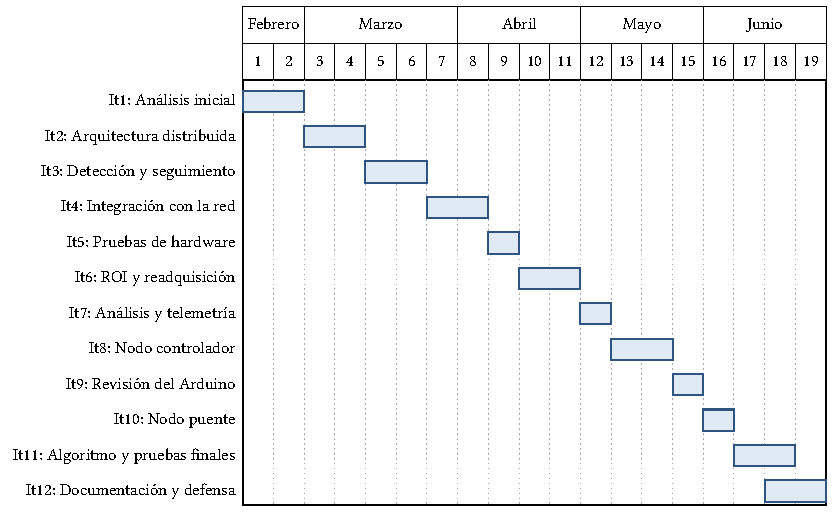
\includegraphics[width=0.8\textwidth]{imaxes/DESARROLLO/gantt_base.pdf}
    \caption{Planificación inicial del proyecto}
    \label{fig:gantt-base}
\end{figure}

A lo largo del proyecto surgieron diversas dificultades que condicionaron el ritmo del desarrollo. Las más relevantes se concentraron en la fase de integración con la red, donde el uso de Docker junto con ROS2 generó una serie de problemas que retrasaron el conseguir un despliegue estable. Asimismo, el hardware presentó fallos intermitentes que, al no manifestarse de forma constante, resultaron difíciles de diagnosticar y consumieron bastante tiempo. Finalmente, durante el desarrollo del algoritmo de control aparecieron fallos no previstos que obligaron a revisar y ajustar el diseño.

El efecto de esas dificultades sobre el calendario se ve en la figura~\ref{fig:gantt-retrasos}, que enfrenta cada iteración con la duración que tenía planificada. Las que más se alargaron fueron la integración con la red y la mejora del algoritmo, y por detrás las pruebas de hardware, mientras que las demás se desplazaron en bloque tras ellas, de forma que el trabajo se cerró siete semanas más tarde de lo previsto, a mediados de agosto, cambiando la fecha de entrega.

\begin{figure}[tbp]
    \centering
    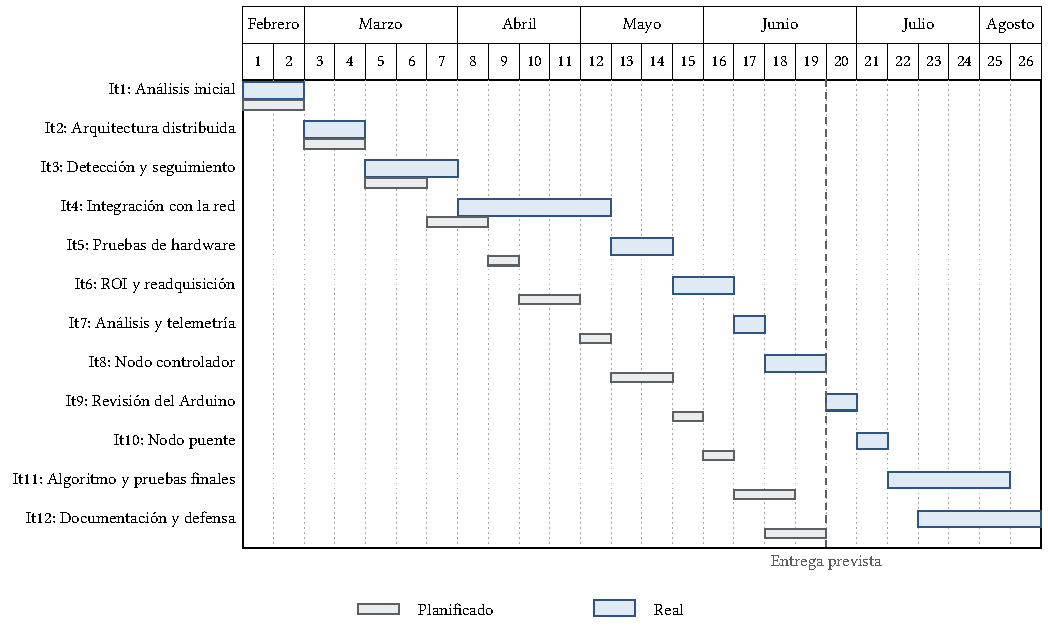
\includegraphics[width=\textwidth]{imaxes/DESARROLLO/gantt_retrasos.pdf}
    \caption{Planificación real del proyecto}
    \label{fig:gantt-retrasos}
\end{figure}


\section{Gestión de archivos}
\label{sec:xestion-arquivos}

Con el fin de garantizar la trazabilidad y la reproducibilidad del trabajo, todos los archivos generados durante el desarrollo del proyecto se han organizado y publicado en un repositorio de acceso público alojado en GitHub~\cite{repogithub}. Dicho repositorio reúne el código fuente de los nodos ROS2 escritos en Python, las definiciones de los mensajes personalizados intercambiados entre nodos, el firmware de Arduino encargado de generar las señales PWM, así como los ficheros de configuración del sistema (el fichero de parámetros en YAML y los ficheros de Docker Compose empleados en el despliegue).

Para ilustrar el funcionamiento del sistema se han grabado y publicado vídeos de las distintas pruebas realizadas, capturados a partir de las grabaciones (sección~\ref{sec:ros2-rosbag}) y accesibles desde el canal de YouTube asociado al proyecto~\cite{canalyoutube}. Este material aporta evidencia visual de los resultados alcanzados.

\section{Recursos}
\label{sec:recursos}

En esta sección se enumeran los recursos hardware, software y humanos que han intervenido en el desarrollo del proyecto.

\subsection{Recursos hardware}

El material empleado se agrupa en tres bloques. El primero es la pista, un circuito de Scalextric con la electrónica que le aplica la tensión, formada por la placa Elegoo Uno R3 y el módulo controlador L293D. El segundo es el equipamiento de visión, con cuatro cámaras web (dos Microsoft LifeCam HD-5000 y dos Logitech Brio 100) y dos placas Raspberry Pi 5, que son las que ejecutan los nodos de captura. El tercero es el ordenador portátil ASUS Vivobook S 14, donde se ejecutaban habitualmente los nodos de control y el nodo de potencia, por lo que es el que tenía la placa conectada por USB. Todo ello se detalla, junto con su coste, en la tabla~\ref{tab:costes_hardware} de la sección~\ref{sec:custos}.

\subsection{Recursos software}

Todo el software empleado en el proyecto es de código abierto o de uso gratuito, por lo que no lleva asociado ningún coste de licencia. El listado completo se detalla en el capítulo de tecnologías; los lenguajes de programación utilizados fueron:

\begin{itemize}
    \item Python, empleado en la implementación de los nodos ROS2 y de toda la lógica de visión y control.
    \item C/C++, utilizado en el firmware de la placa Arduino encargado de interpretar los comandos de velocidad y generar las señales PWM.
\end{itemize}

\subsection{Recursos humanos}

Durante el desarrollo del proyecto, el alumno ha asumido de forma íntegra los distintos roles que intervienen en un proceso de ingeniería del software:

\begin{itemize}
    \item \textbf{Jefe de proyecto}: planifica y coordina las fases del desarrollo y actúa como enlace con los tutores.
    \item \textbf{Analista}: recopila y modela los requisitos del sistema y define las especificaciones funcionales.
    \item \textbf{Arquitecto de software}: diseña la arquitectura distribuida, selecciona las tecnologías y establece la estructura modular basada en nodos.
    \item \textbf{Programador}: implementa las funcionalidades, integra los distintos nodos y realiza tareas de optimización.
    \item \textbf{Responsable de pruebas}: diseña y ejecuta las pruebas necesarias para verificar el correcto funcionamiento del sistema.
\end{itemize}

\section{Estimación de costes}
\label{sec:custos}

En este apartado se estima el coste total del proyecto a partir de los recursos materiales y humanos empleados. Los recursos software no generan coste alguno, ya que todo el software utilizado es libre o gratuito.

El coste de los recursos hardware se recoge en la tabla~\ref{tab:costes_hardware}. Todo el material aparece a precio de compra salvo el ordenador portátil, que no se adquirió para este trabajo, sino que es un equipo personal empleado también para otras tareas. Su coste se estima por amortización, repartiendo los 1.600~\euro{} que costó entre una vida útil de cuatro años, lo que supone 1,10~\euro{} al día y un total de 197~\euro{} por los 180 días que duró el desarrollo.

\begin{table}[tbp]
    \centering
    \estilotabla
    \caption{Costes derivados del hardware}
    \label{tab:costes_hardware}
    \begin{tabular}{lc}
        \toprule
        \rowcolor{ArqAzulClaro}
        \textbf{Dispositivo} & \textbf{Coste} \\
        \midrule
        Elegoo Uno R3                         & 19,99 \euro   \\
        Controlador de Motores L293D          & 5,81 \euro    \\
        Microsoft LifeCam HD-5000 ($\times$2) & 70,42 \euro   \\
        Logitech Brio 100 ($\times$2)         & 80,00 \euro   \\
        Circuito Scalextric EVOLUTION         & 119,99 \euro  \\
        Raspberry Pi 5 ($\times$2)            & 180,00 \euro  \\
        Router TP-Link Archer AX55            & 89,99 \euro   \\
        Adaptador de red Archer T3U ($\times$2) & 39,98 \euro \\
        ASUS Vivobook S 14 (amortización)     & 197,00 \euro  \\
        \midrule
        \textbf{Total} & \textbf{803,18 \euro} \\
        \bottomrule
    \end{tabular}
\end{table}

Respecto a los recursos humanos, el desarrollo se llevó a cabo a lo largo de aproximadamente 180 días, con una dedicación media en torno a las 3 horas diarias, aunque hubo días de un periodo mayor y otros en los que hubo menos, lo que supone un total cercano a las 540 horas de trabajo efectivas. El esfuerzo se distribuyó entre los distintos roles asignando a cada uno una carga horaria acorde con sus responsabilidades, concentrándose la mayor parte del tiempo en las tareas de programación. El desglose de horas y costes se muestra en la tabla~\ref{tab:costes_humanos}.

\begin{table}[tbp]
    \centering
    \estilotabla
    \caption{Desglose de horas y costes de los recursos humanos}
    \label{tab:costes_humanos}
    \begin{tabular}{lccc}
        \toprule
        \rowcolor{ArqAzulClaro}
        \textbf{Rol} & \textbf{Horas} &
        \textbf{Coste/hora (\euro/h)} & \textbf{Coste total (\euro)} \\
        \midrule
        Jefe de proyecto        & 55  & 60 & 3\,300  \\
        Analista                & 45  & 45 & 2\,025  \\
        Arquitecto de software  & 50  & 55 & 2\,750  \\
        Programador             & 320 & 50 & 16\,000 \\
        Responsable de pruebas  & 35  & 40 & 1\,400  \\
        Documentador            & 35  & 40 & 1\,400  \\
        \midrule
        \textbf{Total} & \textbf{540} & --- & \textbf{26\,875} \\
        \bottomrule
    \end{tabular}
\end{table}

Sumando el coste de los recursos hardware (tabla~\ref{tab:costes_hardware}) y el de los recursos humanos (tabla~\ref{tab:costes_humanos}), y teniendo en cuenta que los recursos software no suponen coste alguno, el coste total estimado del proyecto asciende a \textbf{27\,481{,}18 \euro}.
 \chapter{Arquitectura y diseño}
\label{chap:arquitectura}


\section{Arquitectura general del sistema}
\label{sec:arquitectura}

El proyecto cuenta con cuatro nodos diferenciados, atendiendo cada uno a un subconjunto de los requisitos totales del proyecto agrupados por funcionalidades:

\begin{itemize}
    \item El modulo de captura y detección de posición
    \item El modulo de control de velocidad
    \item El modulo de actuación sobre el hardware
    \item El modulo de visualización
\end{itemize}

Esto permite el aislamiento del proyecto en sistemas independientes que se interconectan, enviando y recibiendo la información necesaria para su correcto funcionamiento através de la red, no pueden compartir un estado de memoria.

El funcionamiento del proyecto se lleva a cabo mediante la ejecución de un conjunto de nodos ROS~2 distribuidos en varias máquinas, que realizan la comunicación entre todos los nodos mediante la publicación y suscripción a \emph{topics} de ROS~2 y de una aplicación ejecutada en un Arduino cuyo hardware está conectado a la pista del Scalextric (ver figura~\ref{fig:arquitectura-general}). 

El \textbf{Modulo de captura y detección} está formado por un nodo cámara por cada cámara que observa el circuito, desplegado dentro de un contenedor Docker sobre la máquina a la que está conectada físicamente. Cada uno de estos nodos captura los fotogramas de su cámara, detecta en ellos los coches presentes en su porción visible del circuito y publica la posición de cada uno de ellos. 

El \textbf{Modulo de control del rail} se compone de un nodo controlador por cada raíl del circuito que, suscrito a las posiciones publicadas para su rail por cada uno de los nodos cámara, reconstruye la trayectoria del coche asignado a su carril y además utilizando las posiciones que recibe aplica un algoritmo cuyo objetivo es obtener el mejor valor del PWM para cada instante con el propósito de reducir al máximo el tiempo por vuelta. Cada uno de los nodos publica el valor de PWM correspondiente a su caril, para vez que el nodo camara procesa un fotograma y publica la ubicación del coche.

El \textbf{Modulo actuación} centraliza en un único nodo la comunicación con el Arduino los valores de PWM publicados por todos los controladores, trasladándoselos a la aplicación Arduino, que aplica la tensión correspondiente a cada carril de la pista a través de un controlador L293D. La comunicación entre este nodo y el Arduino se lleva a cabo mediante un puerto serie USB conectado al Arduino.

El \textbf{Modulo de visualización y logging} se compone de un nodo de captura que se suscribe a la información de telemetría publicada por el resto del sistema y la almacena dentro de un bag de ROS2. Por otro lado existe un nodo de visualización que permite al usuario supervisar el estado de la carrera en directo y luego en diferido acceder a un analisis de las estadisticas, apartir del bag que genera el otro nodo. 

\begin{figure}[tbp]
    \centering
    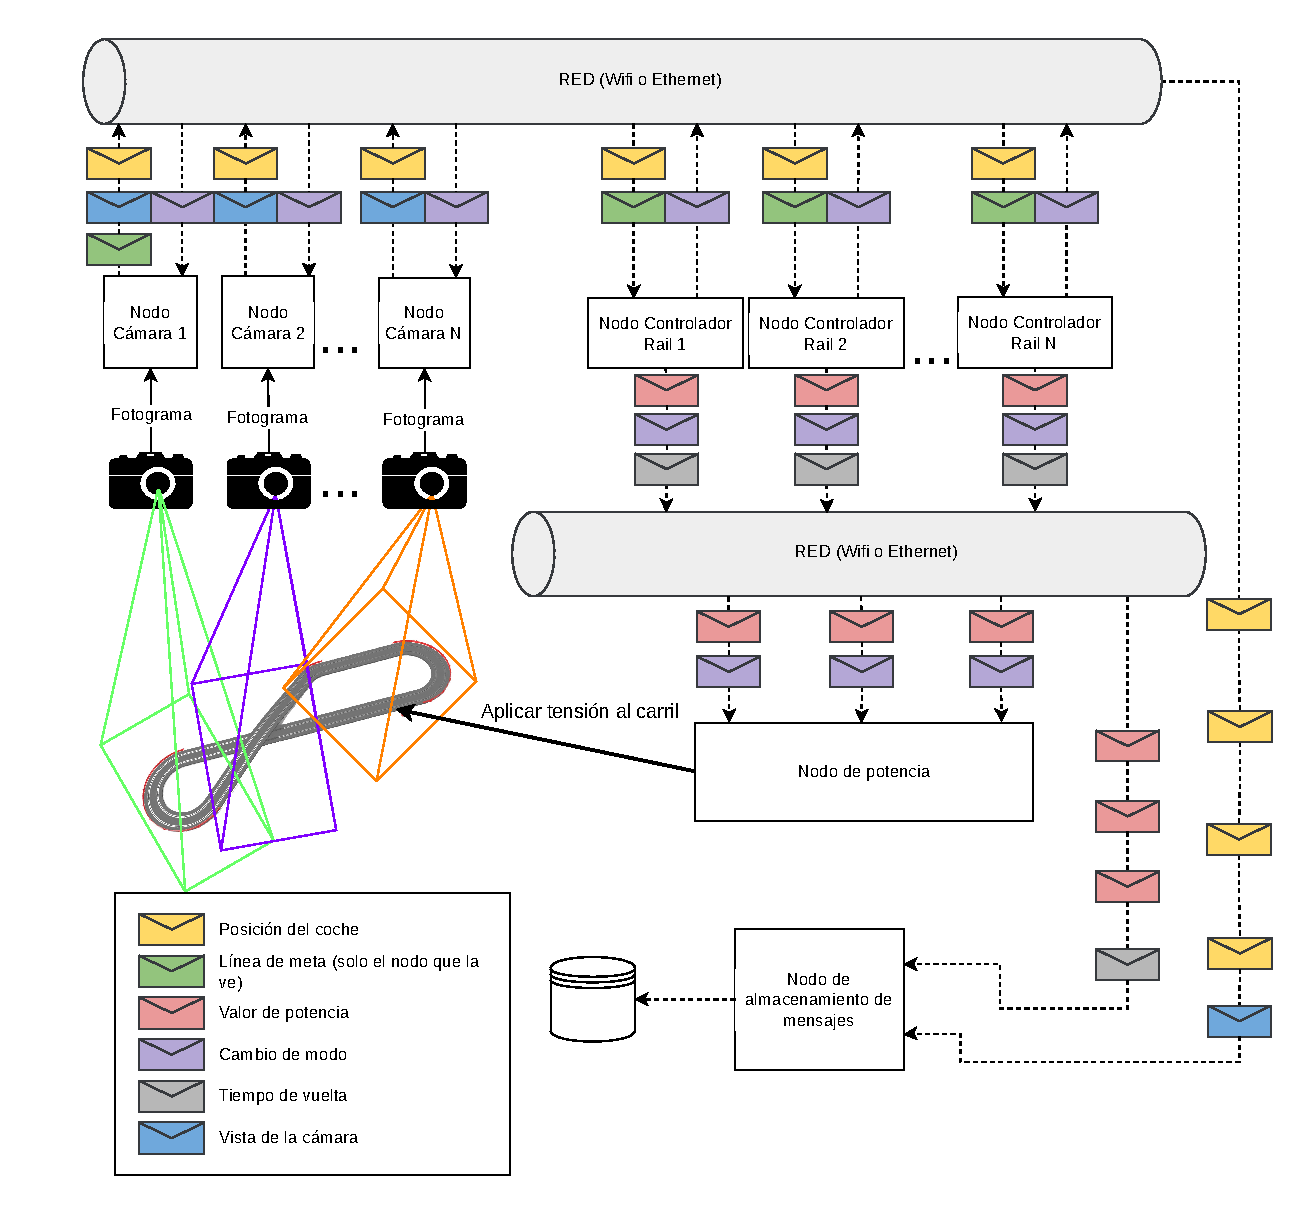
\includegraphics[width=1\textwidth]{imaxes/ARQUITECTURA/Arquitectura_General_Sistema.pdf}
    \caption{Arquitectura general del sistema pensado para el control distribuido de coches tipo scalextric con visión por computado}
    \label{fig:arquitectura-general}
\end{figure}

\section{Modelo de datos}
\label{sec:modelo_datos}

\section{Modos funcionamiento}
\label{sec:modos_funcionamiento}

\section{Algoritmo}
\label{sec:algoritmo}

\section{Intercambio de información(Qos)}
\label{sec:intercambio_informacion}

\section{Modelo concurrente}
\label{concurrencia}

 %\chapter{Implementación del diseño}
%\label{chap:implementacion}
%
%\lettrine{E}{N} este capítulo se describe cómo se ha implementado la arquitectura definida en el capítulo~\ref{chap:arquitectura}. Se detalla como se paso la arquitectura a nodos de ROS~2, la estructura interna de cada uno de ellos, las decisiones tomadas al programarlos y las desviaciones que aparecieron respecto al diseño inicial.
%
%\section{Configuración y despliegue}
%\label{sec:configuracion_despliegue}
%
%El número de cámaras y de coches, y su reparto entre máquinas, se decide al desplegar el sistema (sección~\ref{sec:despliegue_sistema}). Esa flexibilidad descansa sobre tres piezas: un fichero de parámetros común, un fichero de lanzamiento por componente y un contenedor que lo ejecuta.
%
%\subsection{Fichero de parámetros}
%\label{subsec:params-yaml}
%
%Toda la configuración se centraliza en \texttt{params.yaml}, compartido por todos los nodos, se puede consultar íntegro en el anexo~\ref{lst:params-yaml}. A pesar de la cantidad de parametros que hay cada nodo declara únicamente los que le interesan y descarta el resto.
%
%En la raíz están los dos parámetros que definen la escala del despliegue. La lista \texttt{coches} enumera los coches del sistema y es la que determina cuántos detectores crea cada cámara, cuántos controladores se levantan y a qué \emph{topics} se suscribe el puente. El bloque \texttt{cars} contiene la configuración propia de cada coche, indexada por su nombre: los colores de sus dos pegatinas (\texttt{stiker\_front} y \texttt{stiker\_back}), que son lo que permite seguir a varios coches a la vez sin confundirlos; el \texttt{carril} físico del circuito donde va el coche y un indicador \texttt{modo\_manual}, que decide si el coche lo controla el sistema o una persona.
%
%El resto de parámetros se agrupa por componente. El bloque \texttt{camera} fija la resolución de trabajo (\texttt{mode}, uno de cinco modos predefinidos que van de $160 \times 120$ a $1280 \times 720$ píxeles), el dispositivo de vídeo (\texttt{device}, que admite tanto un índice numérico como la ruta \texttt{/dev/videoN}), el modo de depuración y la anchura de la franja en la que se busca al coche (\texttt{mascara\_kernel\_size}); su subbloque \texttt{detection} ajusta la detección por color con el color de la meta, el núcleo de la limpieza morfológica y el área mínima de un contorno válido. El bloque \texttt{controller} fija los límites del perfil de velocidad —\texttt{minimum\_speed}, el PWM con el que arranca la carrera, y \texttt{maximum\_speed}, el techo del aprendizaje— y la separación mínima entre puntos de la trayectoria base. El bloque \texttt{arduino} recoge el puerto serie, su velocidad de transmisión y el PWM constante que se aplica durante la calibración.
%
%Todos estos parametros gracias al funcionamientode ROS2 algunos se pueden cambiar en caliente. Lo que permite ajustar el sistema sin necesidad de tener que relanzar todo el sistema.
%
%\subsection{Ficheros de lanzamiento}
%\label{subsec:launch-files}
%
%Cada nodo tiene su propio fichero de lanzamiento (sección~\ref{sec:ros2-launch}), y todos siguen el mismo patrón. Primero leen el fichero de parámetros común y después crean los nodos necesarios y le asignan un espacio de nombres.
%
%El del nodo de captura (\ref{lst:camera-launch}) es el más simple. Recibe como argumentos el identificador del nodo y el dispositivo de vídeo, y los inyecta como parámetros junto con la ruta al fichero común, \ref{subsec:params-yaml}.
%
%El número de nodos de control y la existencia de un nodo puente, se decide dentro del launch de forma dinámica justo antes del lanzamiento. Recorre la lista \texttt{coches} del fichero de parámetros y crean un controlador por cada uno, filtrando por el indicador \texttt{modo\_manual}. El principal (anexo~\ref{lst:brain-launch}) se queda con los coches autónomos y añade el nodo puente, que solo tiene sentido si hay que controlar algún coche. El de carrera manual (anexo~\ref{lst:manual-launch}) se queda con los manuales y no arranca el puente, no sé publica el mensaje de potencia \ref{sec:modelo_datos_ros2}. Sus controladores se levantan con el modo manual activo, permite obtener información pero no sé publica ningún valor de voltaje.\footnote{Cada controlador recibe un nombre de nodo único derivado del nombre del coche y del modo, porque el controlador genera sus ficheros de \emph{log} con el nombre del nodo y dos nodos homónimos se pisarían.}
%
%Como ambos ficheros filtran la misma lista por criterios opuestos, una carrera mixta se consigue levantando los dos a la vez.
%
%Todos los nodos se declaran con reinicio automático y un retardo entre intentos. Si un nodo cae durante una sesión, el sistema lo relanza y este se reincorpora por sí solo gracias al descubrimiento del \emph{middleware}, comportamiento que se valida en la prueba de tolerancia a fallos de la sección~\ref{subsec:prueba-tolerancia}.
%
%\subsection{Despliegue en contenedores}
%\label{subsec:despliegue-docker}
%
%Cada componente se despliega en un contenedor Docker construido sobre una imagen común, derivada de la imagen oficial de ROS~2 y ampliada con las bibliotecas de visión y de comunicación serie. Una máquina solo necesita, por tanto, Docker y conectividad de red. No hace falta instalar ROS~2 ni ninguna dependencia en el anfitrión, cumpliendo lo exigido en \ref{sec:configuracion_despliegue}.
%
%Los tres ficheros \emph{compose} comparten la misma configuración base. Los contenedores usan la pila de red y la memoria compartida del anfitrión, y fijan el mismo identificador de dominio (sección~\ref{sec:dds-qos}). Con la red del anfitrión los nodos se descubren entre máquinas. La memoria compartida es lo que permite que, cuando dos nodos coinciden en la misma máquina, la capa de comunicación de ROS~2 lo detecte y los comunique directamente, sin pasar por la pila de red. Todos montan además el paquete desde el anfitrión, para conservar al parar el contenedor los ficheros que escriben los nodos (cachés de trayectoria y registros del algoritmo), y fijan la zona horaria, ya que la imagen base trabaja en UTC.
%
%El del nodo de captura (listado~\ref{lst:compose-camera}) recibe como variables de entorno el identificador del nodo y la ruta a su dispositivo, y se los traslada al fichero de lanzamiento. El del cerebro (anexo~\ref{lst:compose-brain}) es el único que mapea el dispositivo serie del Arduino dentro del contenedor. El de modo manual (anexo~\ref{lst:compose-manual}) es idéntico al anterior salvo por ese mapeo, que no incluye: así el contenedor arranca aunque el Arduino ni siquiera esté conectado.
%
%\begin{lstlisting}[language=Python, caption={Fichero de lanzamiento del nodo de captura (\texttt{launch/CameraLaunch.py}).}, label={lst:camera-launch}]
%from launch import LaunchDescription
%from launch_ros.actions import Node
%from launch_ros.substitutions import FindPackageShare
%from launch.substitutions import PathJoinSubstitution, LaunchConfiguration
%from launch.actions import DeclareLaunchArgument
%
%def generate_launch_description():
%
%    # Cargamos el fichero de configuracion: params.yaml
%    params_file = PathJoinSubstitution([
%        FindPackageShare('image_processor_pkg'),
%        'config',
%        'params.yaml'
%    ])
%
%    # Obtenemos el nombre del nodo
%    node_id = DeclareLaunchArgument(
%        'node_id',
%        default_value='camera_00',
%        description='Nombre con el que se identifica al nodo en la red ROS2'
%    )
%
%    # Nombre de la camara que queremos levantar
%    camera_name = DeclareLaunchArgument(
%        'camera_name',
%        default_value='0',
%        description='ID numerico (0) o ruta entera de la camara (/dev/video0)'
%    )
%
%    return LaunchDescription([
%        camera_name,
%        node_id,
%        Node(
%            package='image_processor_pkg',
%            executable='CameraNode.py',
%            namespace=LaunchConfiguration('node_id'),
%            parameters=[
%                params_file,
%                {'camara_id': LaunchConfiguration('node_id')},
%                {'camera.device': LaunchConfiguration('camera_name')}
%            ],
%            respawn=True,
%            respawn_delay=2.0
%        )
%    ])
%\end{lstlisting}
%
%\begin{lstlisting}[caption={Fichero \emph{compose} del nodo de captura, desplegado en cada máquina con cámara (\texttt{docker-compose-camera.yml}).}, label={lst:compose-camera}]
%services:
%  emisor:
%    build: .
%    network_mode: "host"
%    privileged: true
%    ipc: "host"
%    environment:
%      - ROS_DOMAIN_ID=42
%      - ROS_LOCALHOST_ONLY=0
%      - NODE_ID=${NODE_ID}
%      - CAMERA_DEV=${CAMERA_DEV}
%      - TZ=Europe/Madrid
%    volumes:
%      - /etc/localtime:/etc/localtime:ro
%      - ./src/image_processor_pkg:/ros2_ws/src/image_processor_pkg
%    command: >
%      bash -c "source /opt/ros/humble/setup.bash &&
%               colcon build --symlink-install &&
%               source install/setup.bash &&
%               ros2 launch image_processor_pkg CameraLaunch.py
%                    camera_name:=${CAMERA_DEV} node_id:=${NODE_ID}"
%\end{lstlisting}
%
%\subsection{Caché de la calibración}
%\label{subsec:cache-calibracion}
%
%Para no repetir la calibración en cada arranque, lo aprendido durante ella se guarda en disco en ficheros JSON. Cada cámara almacena los puntos de trayectoria de cada coche y cada controlador la trayectoria base que construye por cámara. Al iniciarse, los nodos comprueban si existe su fichero y, en caso afirmativo, lo cargan y pasan directamente a modo carrera. Esto reduce el tiempo de puesta en marcha cuando ni las cámaras ni el circuito se han movido. Si se ordena una recalibración, los datos se descartan.
%
%\section{Modelo de ejecución concurrente}
%\label{concurrencia}
%
%La concurrencia dentro del nodo que exige la arquitectura (sección~\ref{sec:concurrencia}) se resuelve con los \emph{executors} y los grupos de \emph{callbacks} de ROS~2, descritos en la sección~\ref{sec:ros2-executors}. Todos los nodos del sistema se ejecutan sobre un \emph{MultiThreadedExecutor} y reparten sus tareas entre varios \emph{MutuallyExclusiveCallbackGroup}.
%
%Para realizar el reparto se decide con un doble criterio. Los \emph{callbacks} que modificar el mismo estado interno van al mismo grupo y en segundo lugar las tareas que son independientes van a grupos separados. Permite garantizar que ninguna tarea espere por otra.
%
%\subsection{Nodo de captura}
%\label{subsec:concurrencia-camara}
%
%Es el nodo con más concurrencia, y la reparte en dos niveles.
%
%Primero tenemos la concurrencia nivel de nodo. Debe realizar dos tareas bien diferenciadas. La primera es el procesamiento de los fotogramas para obtener las posiciones de los coches y en segundo lugar debe generar las imagenes de debug. Es por ello que cada uno tiene su propio grupo (\ref{fig:executor-multihilo}). A parte de estos dos grupos se añade un hilo extra que atiende al grupo por defecto de ROS~2, que recoge el resto de los \emph{callbacks}. Permitiendo modificar parametros en caliente y avisar al sistema de que hay que activar el modo de calibración.
%
%\begin{figure}[H]
%    \centering
%    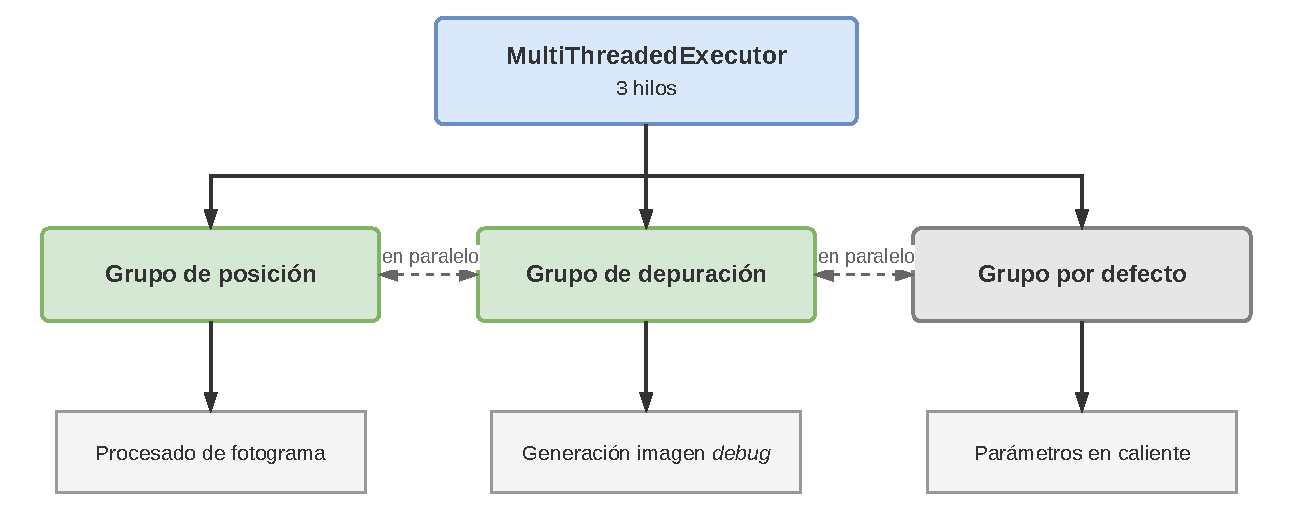
\includegraphics[width=\textwidth]{imaxes/IMPLEMENTACION/multithread_nodo_camara.pdf}
%    \caption{Esquema que permite ver el nivel de concurrencia a nivel de nodo dentro del nodo camara}
%    \label{fig:executor-multihilo}
%\end{figure}
%
%Para optimizar el tener que buscar dentro de un fotograma varios coches implica utilizar también un patrón de concurrencia. En este caso se eligió el patrón productor-consumidor, \ref{fig:modelo-hilos-camara}. El  hilo consumidor coge los fotogramas que la camara recibe cada \qty{33}{\milli\second}, equivalente a la frecuencia máxima de captura de las cámaras empleadas. Después el hilo consumidor se implementa usando un \emph{timer} de ROS2 que coge el último fotograma y lanza su procesamiento sobre un \emph{ThreadPool} con un trabajador por coche: como la búsqueda de cada coche es independiente de las demás, todas se ejecutan concurrentemente sobre el mismo fotograma y el consumidor espera a que terminen antes de darlo por procesado. Se usa un \emph{flag} que impide que un nuevo disparo se solape con un procesamiento en curso. Si el análisis se prolonga, los disparos intermedios se descartan en lugar de encolarse.
%
%\begin{figure}[H]
%    \centering
%    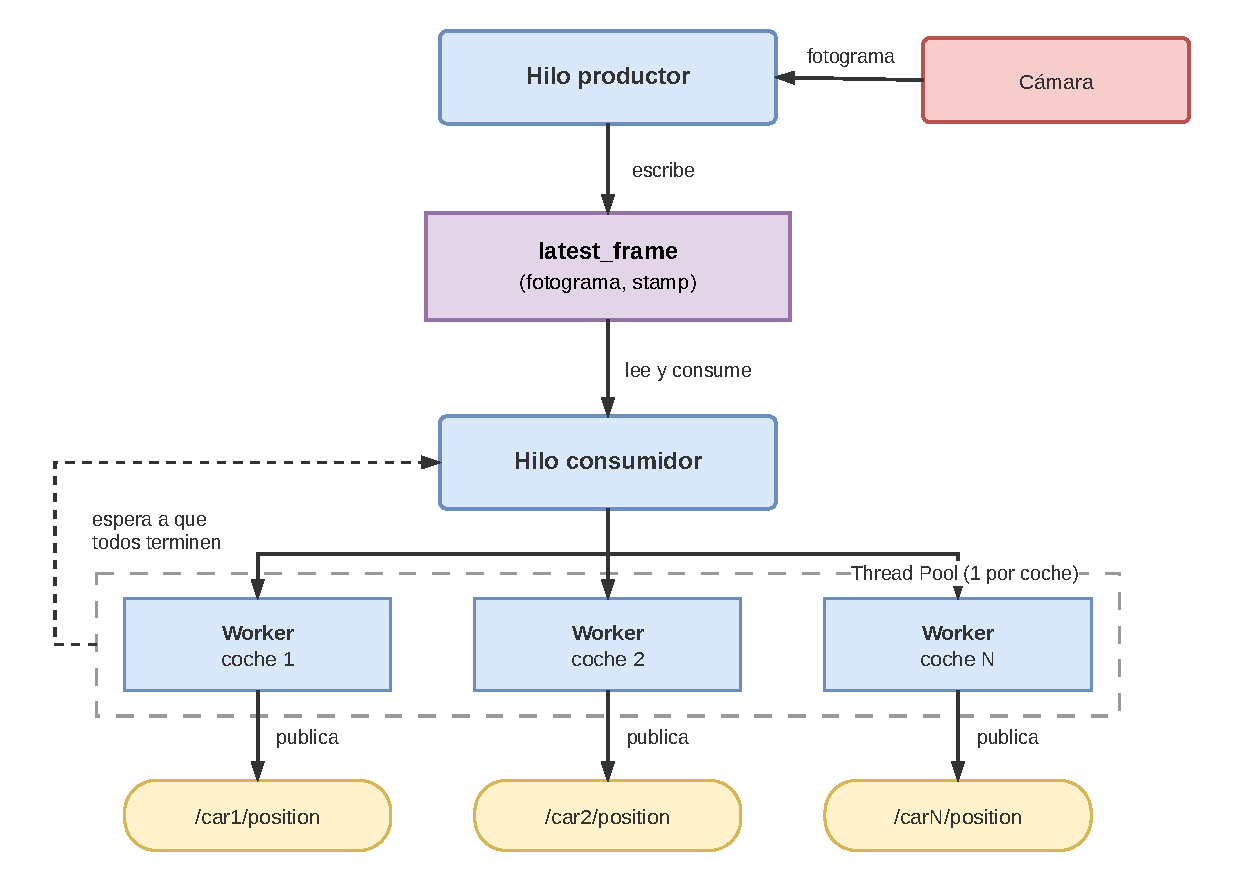
\includegraphics[width=0.75\textwidth]{imaxes/IMPLEMENTACION/productor_consumidor_nodo_camara.pdf}
%    \caption{Modelo de ejecución multihilo productor-consumidor utilizado dentro
%             del nodo de cámara.}
%    \label{fig:modelo-hilos-camara}
%\end{figure}
%
%\subsection{Nodo de control de carril}
%\label{subsec:concurrencia-controlador}
%
%El controlador solo necesita concurrencia a nivel de nodo. Recibe tres \emph{callbacks} distintos: la posición del coche, la orden de cambio de modo y la línea de meta. Como los tres modifican el mismo estado interno, se asignan a un único grupo, el estado del algoritmo queda de este modo en manos de un solo hilo a la vez. Junto a él se conserva el grupo por defecto de ROS~2, atendido por un segundo hilo, que deja disponible la actualización de parámetros en caliente sin interrumpir el control (figura~\ref{fig:concurrencia-controlador}).
%
%\begin{figure}[H]
%    \centering
%    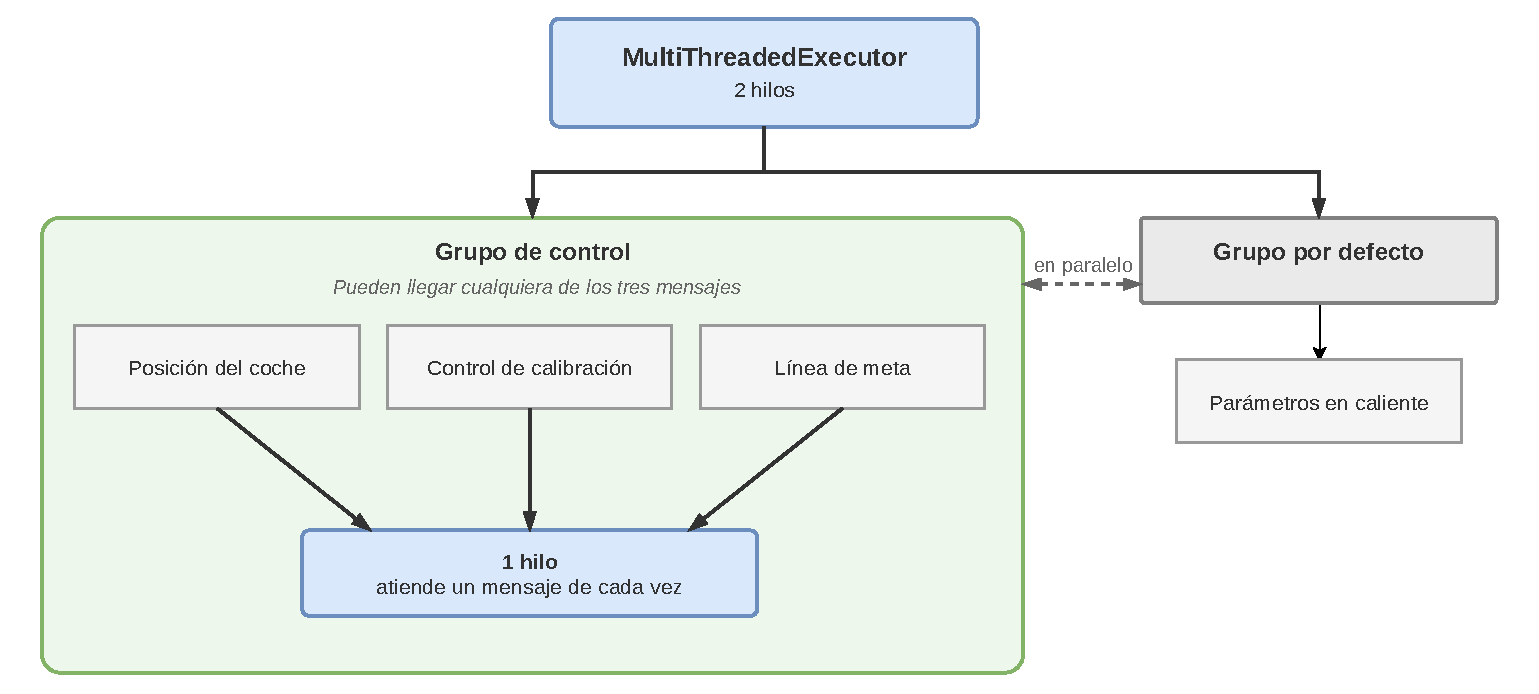
\includegraphics[width=\textwidth]{imaxes/IMPLEMENTACION/multithread_nodo_controlador.pdf}
%    \caption{Modelo de ejecución multihilo a nivel de nodo utilizado dentro del nodo de control de rail}
%    \label{fig:concurrencia-controlador}
%\end{figure}
%
%\subsection{Nodo de actuación}
%\label{subsec:concurrencia-puente}
%
%El puente crea un grupo por cada controlador desplegado, ya que cada uno publica en su propio \emph{topic}, más un grupo para las suscripciones de calibración y el grupo por defecto (figura~\ref{fig:concurrencia-puente}). Así, si el mensaje de un carril se demora no impide recibir y tratar los del resto.
%
%Esta concurrencia en la recepción no puede trasladarse al envío. Existe un único Arduino y un único puerto serie, de modo que el acceso al hardware está necesariamente serializado. La serialización la impone la propia interfaz de comunicación (sección~\ref{subsec:actuacion-interfaz}).
%
%\begin{figure}[H]
%    \centering
%    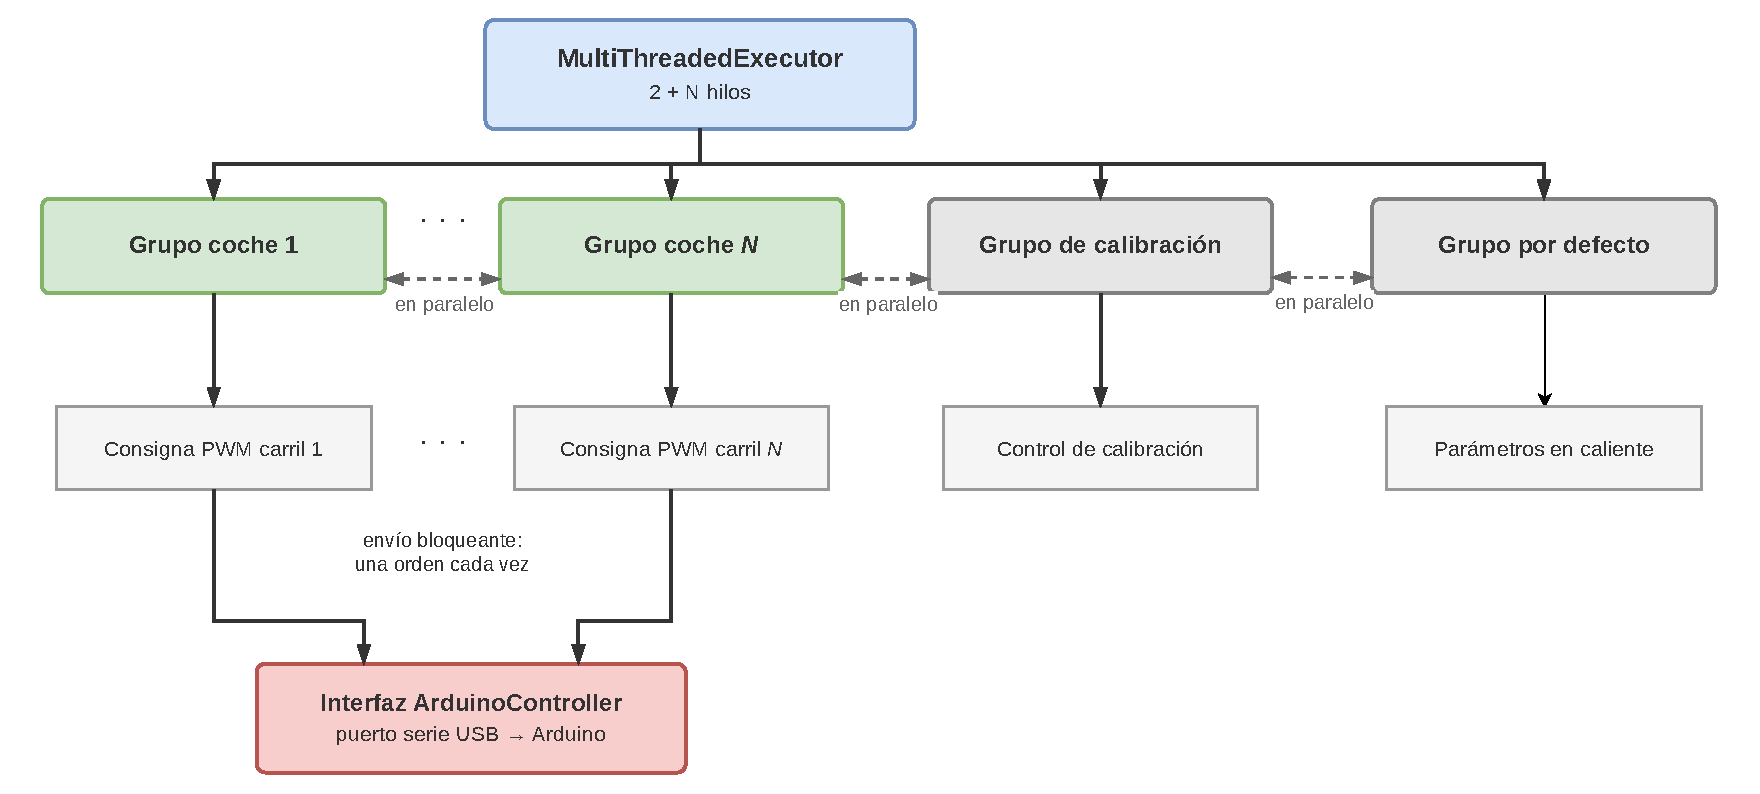
\includegraphics[width=0.9\textwidth]{imaxes/IMPLEMENTACION/multithread_nodo_puente.pdf}
%    \caption{Modelo de ejecución multihilo a nivel de nodo utilizado dentro del nodo puente}
%    \label{fig:concurrencia-puente}
%\end{figure}
%
%\section{Nodo de captura y detección}
%\label{sec:nodo-camara}
%
%El nodo de captura (sección~\ref{sec:arquitectura}) se divide en dos componentes: el nodo de ROS~2, que gestiona la comunicación y los modos de funcionamiento, y un objeto que encapsula la operaciones de visión artificial con las que se obtiene el centroide de cada pegatina. Logrando desacoplar el procesamiento de imagen de la comunicación.
%
%\subsection{Detección de las pegatinas por color}
%\label{subsec:deteccion-etiquetas}
%
%\begin{figure}[H]
%    \centering
%    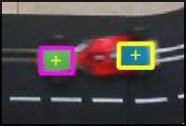
\includegraphics[width=0.6\textwidth]{imaxes/IMPLEMENTACION/deteccion_2_pegatinas.png}
%    \caption{Ejemplo de detección de las dos pegatinas del coche}
%    \label{fig:deteccion-2-pegatinas}
%\end{figure}
%
%La detección hereda el procedimiento del trabajo de Mario López~\cite{tfgmario}. El fotograma se convierte al espacio HSV, que resiste mejor las variaciones de iluminación, y se genera una máscara binaria por pegatina con los píxeles que caen dentro del rango de su color. Están predefinidos para cada uno de los siete colores admitidos. Sobre cada máscara se encadenan una apertura morfológica, que elimina los píxeles aislados, y un cierre morfológico, que rellena los huecos de las regiones válidas.
%
%Se extraen entonces los contornos externos y se toma el de mayor área, descartándolo si no supera un área mínima configurable. De este proceso se obtiene el rectángulo delimitador y el centroide de la pegatina, el significado para cada pegatina se describió en la sección~\ref{sec:arquitectura}. La figura~\ref{fig:deteccion-color} recorre estas etapas sobre un fotograma real.
%
%\begin{figure}[tbp]
%    \centering
%    \begin{subfigure}[b]{0.48\textwidth}
%        \centering
%        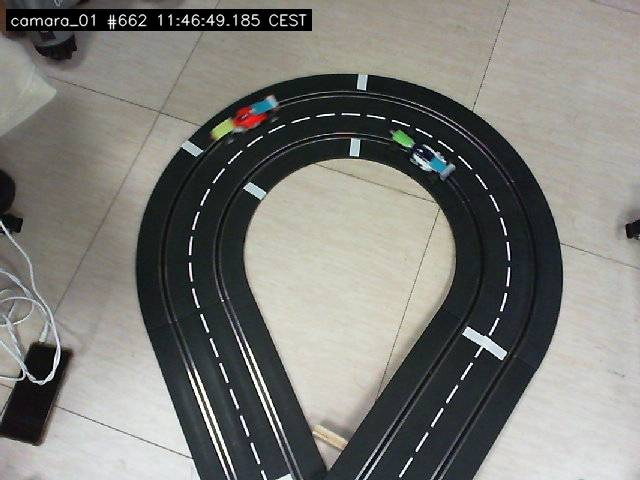
\includegraphics[width=\textwidth]{imaxes/IMPLEMENTACION/det_color_a_original.png}
%        \caption{Fotograma capturado por la cámara}
%        \label{fig:deteccion-color-a}
%    \end{subfigure}
%    \hfill
%    \begin{subfigure}[b]{0.48\textwidth}
%        \centering
%        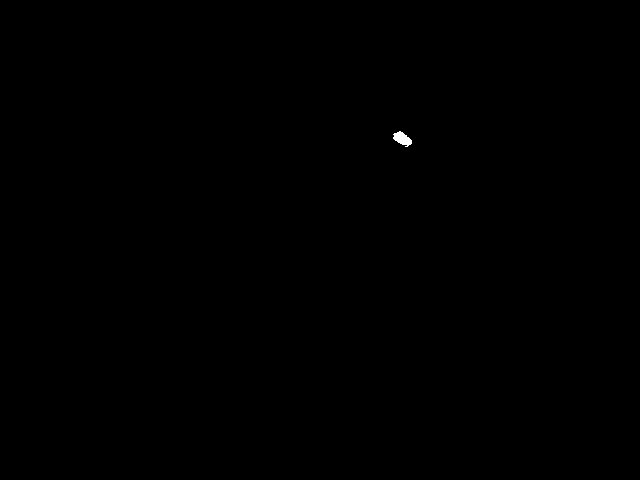
\includegraphics[width=\textwidth]{imaxes/IMPLEMENTACION/det_color_b_mascara.png}
%        \caption{Máscara del color de la pegatina verde delantera del coche azul}
%        \label{fig:deteccion-color-b}
%    \end{subfigure}
%
%    \vspace{0.7em}
%    \begin{subfigure}[b]{0.34\textwidth}
%        \centering
%        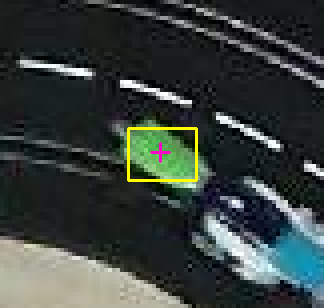
\includegraphics[width=\textwidth]{imaxes/IMPLEMENTACION/det_color_c_resultado.png}
%        \caption{Rectángulo y centroide detectados después de realizar las operaciones pertinentes}
%        \label{fig:deteccion-color-c}
%    \end{subfigure}
%    \caption{Ejemplo del proceso de detección que realiza el nodo camara para detectar una de las pegatinas del coche}
%    \label{fig:deteccion-color}
%\end{figure}
%
%\subsection{Diferencias entre calibración y carrera}
%\label{subsec:modos-funcionamiento}
%
%El nodo implementa los dos modos descritos en la sección~\ref{sec:modos_funcionamiento}, y la diferencia entre ambos está en la región del fotograma sobre la que busca.
%
%En calibración, cada detección de la pegatina delantera se añade a la lista que reconstruye la trayectoria del coche. Basta con la delantera, que es la que da una trayectoria limpia~\cite{tfgadrian}. Esto es porque la trasera puede quedar oculta a ratos y la ruta base debe registrarse sin interrupciones. Al mantener una trayectoria por coche, la cámara puede filtrar por carril en carrera y dos coches pueden compartir el color de la pegatina trasera. Durante todo este proceso se busca sobre el fotograma completo como el que se puede ver \ref{fig:deteccion-color-a}, es por ello que las pegatinas delanteras sí que tienen que ser de diferente color.
%
%La calibración termina por coche, no para todo el sistema. El nodo se suscribe al \emph{topic} de calibración de cada coche configurado y, al recibir el aviso de que uno ha completado su vuelta, genera su máscara con los puntos acumulados. Desde ese momento la búsqueda de ese coche queda restringida a una franja alrededor del recorrido conocido, como recoge la figura~\ref{fig:mascara-trayectoria}.
%
%\begin{figure}[tbp]
%    \centering
%    \begin{subfigure}[b]{0.32\textwidth}
%        \centering
%        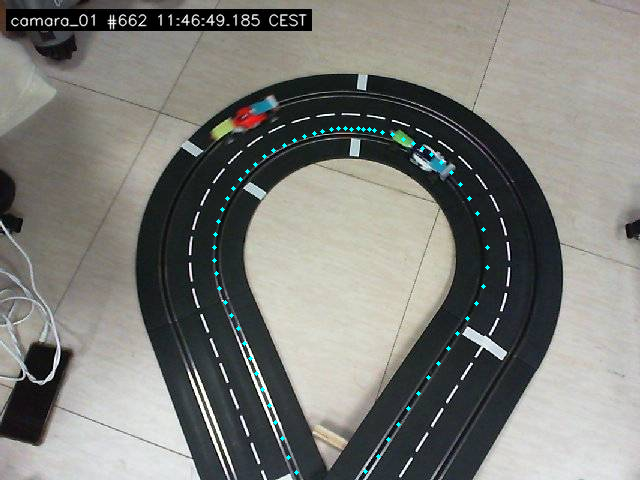
\includegraphics[width=\textwidth]{imaxes/IMPLEMENTACION/mascara_a_puntos.png}
%        \caption{Posiciones acumuladas durante la vuelta de calibración}
%        \label{fig:mascara-trayectoria-a}
%    \end{subfigure}
%    \hfill
%    \begin{subfigure}[b]{0.32\textwidth}
%        \centering
%        
\includegraphics[width=\textwidth]{imaxes/IMPLEMENTACION/mascara_b_mascara.png}
%        \caption{Máscara generada a partir de la posición que sigue el coche}
%        \label{fig:mascara-trayectoria-b}
%    \end{subfigure}
%    \hfill
%    \begin{subfigure}[b]{0.32\textwidth}
%        \centering
%        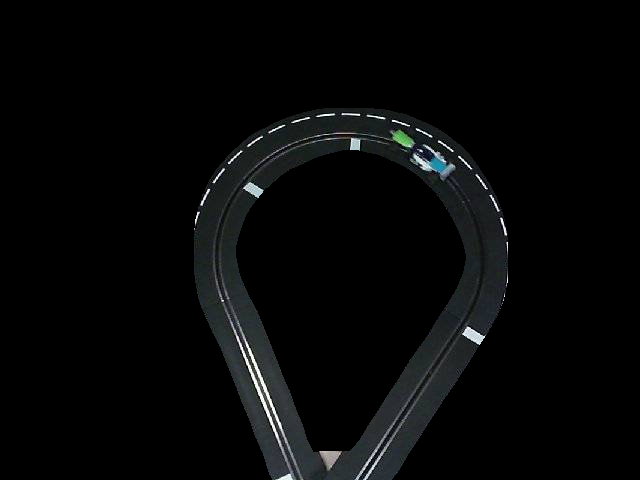
\includegraphics[width=\textwidth]{imaxes/IMPLEMENTACION/mascara_c_filtrado.png}
%        \caption{Fotograma filtrado después de aplicar la mascara generada durante la calibración}
%        \label{fig:mascara-trayectoria-c}
%    \end{subfigure}
%    \caption{Ejemplo de proceso de generación de la máscara de trayectoria para un coche. Deja fuera el carril contrario, con lo que el coche que circula por él deja de ser un falso positivo posible.}
%    \label{fig:mascara-trayectoria}
%\end{figure}
%
%\subsection{Seguimiento mediante región de interés}
%\label{subsec:seguimiento-roi}
%
%En carrera la búsqueda se restringe a una región de interés de $150 \times 150$ píxeles centrada en la posición predicha para el coche. La predicción es la extrapolación lineal que introdujo Mario López~\cite{tfgmario}. Conocidas las dos últimas posiciones, el centro de la región es la actual más el vector de movimiento del último fotograma.
%
%Sobre ella se aplica además la máscara de trayectoria, de modo que solo sobreviven los píxeles que pertenecen a la vez a la región y a las proximidades del carril; la intersección de ambos filtros procede también de los trabajos previos~\cite{tfgmario,tfgadrian}. La detección de las pegatinas (\ref{subsec:deteccion-etiquetas}) se realiza sobre esa imagen reducida, se puede ver un ejemplo en \ref{fig:roi-filtrado}. El problema que presenta hacerlo de esta manera es que sus coordenadas son relativas a la región y hay que trasladarlas al sistema de referencia de la cámara antes de publicarlas.
%
%\begin{figure}[tbp]
%    \centering
%    \begin{subfigure}[b]{0.55\textwidth}
%        \centering
%        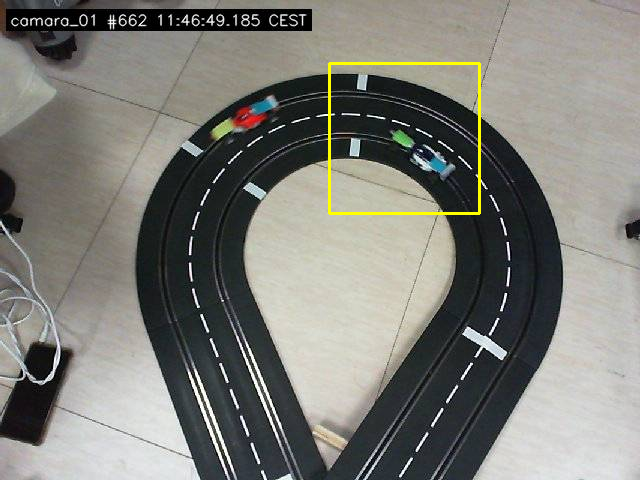
\includegraphics[width=\textwidth]{imaxes/IMPLEMENTACION/roi_a_recuadro.png}
%        \caption{Región de interés marcada sobre todo el fotograma}
%        \label{fig:roi-filtrado-a}
%    \end{subfigure}
%    \hfill
%    \begin{subfigure}[b]{0.38\textwidth}
%        \centering
%        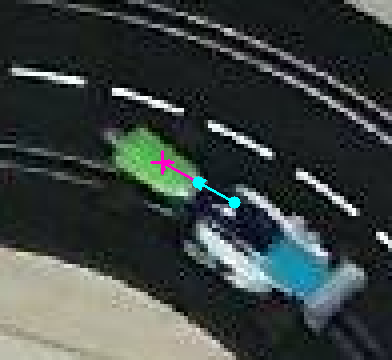
\includegraphics[width=\textwidth]{imaxes/IMPLEMENTACION/roi_b_extrapolacion.png}
%        \caption{Extrapolación de la posición}
%        \label{fig:roi-filtrado-b}
%    \end{subfigure}
%
%    \vspace{0.7em}
%    \begin{subfigure}[b]{0.32\textwidth}
%        \centering
%        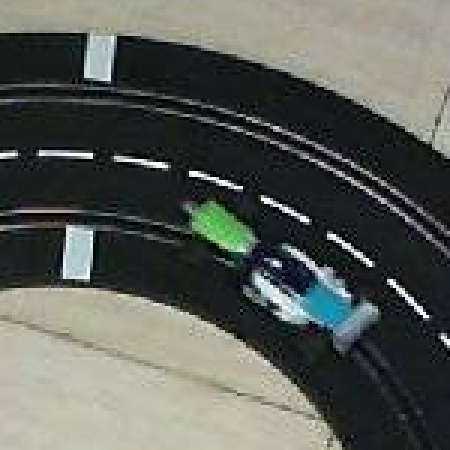
\includegraphics[width=\textwidth]{imaxes/IMPLEMENTACION/roi_c_recorte.png}
%        \caption{Recorte de la región}
%        \label{fig:roi-filtrado-c}
%    \end{subfigure}
%    \hspace{0.04\textwidth}
%    \begin{subfigure}[b]{0.32\textwidth}
%        \centering
%        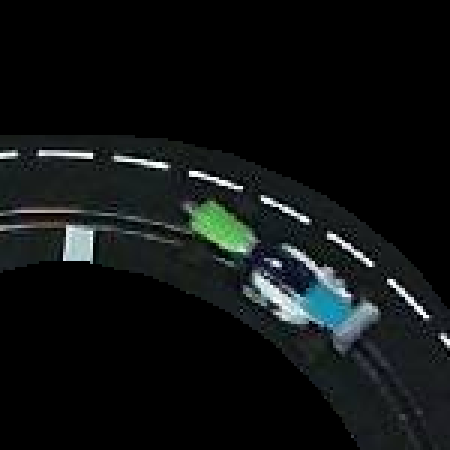
\includegraphics[width=\textwidth]{imaxes/IMPLEMENTACION/roi_d_filtrado.png}
%        \caption{Región tras la intersección entre la mascara y el ROI}
%        \label{fig:roi-filtrado-d}
%    \end{subfigure}
%    \caption{Explicación del proceso de obtención del ROI y aplicación dentro del sistema. En el detalle, las dos flechas encadenadas son el desplazamiento medido entre los dos últimos fotogramas. La cruz marca la posición predicha, que en este fotograma cae a 1,6 píxeles de la real. El último panel es lo único que llega al detector de color.}
%    \label{fig:roi-filtrado}
%\end{figure}
%
%\subsection{Readquisición del seguimiento}
%\label{subsec:readquisicion}
%
%Las oclusiones son habituales en un circuito de Scalextric~\cite{tfgmario}, y un derrape brusco puede alejar el coche de la posición predicha. En ambos casos la detección fracasa y hay que recuperar el seguimiento.
%
%La estrategia es ampliar progresivamente la zona de búsqueda. Cada fotograma sin detección incrementa el tamaño de la región en 50 píxeles, hasta abarcar como máximo la imagen completa. Los trabajos previos pasaban de golpe a examinar toda la proximidad de la trayectoria; el crecimiento gradual acota el coste de los fotogramas inmediatamente posteriores a la pérdida.
%
%Al perder el seguimiento se descartan las posiciones anteriores, como ya hacía Mario López~\cite{tfgmario}, para que la extrapolación no combine un punto previo a la pérdida con el primero posterior y sitúe la región lejos del coche. La primera detección tras readquirir centra la región sobre la posición encontrada.
%
%\subsection{Detección de la línea de meta}
%\label{subsec:deteccion-meta}
%
%La línea de meta se señaliza con una etiqueta alargada de un color reservado que atraviesa la pista. Se detecta una sola vez, al arrancar el nodo, porque su posición no cambia durante la carrera.
%
%El procedimiento empleado para la detección de la línea de meta es el de Adrián Rego~\cite{tfgadrian}. Al igual que en la detección de las pegatinas, el fotograma se convierte al espacio de color HSV y se genera una máscara binaria con el rango del color reservado para la meta (se puede cambiar desde el fichero de configuración \ref{subsec:params-yaml}), de forma que se genera una mascara binaria con los píxeles de la etiqueta. Sobre está se aplica un cierre morfólogico con un tamaño de \emph{kernel} muy grande, porque los raíles y las ranuras de la pista atraviesan la etiqueta y la fragmentan en trozos que hay que unir en una única región. Sobre está región se calcula el rectángulo de área mínima que lo encierra, el cual, a diferencia del rectángulo delimitador convencional, puede estar rotado y se adapta así a la orientación real de la linea de meta. De sus cuatro vértices se identifican los dos lados cortos comparando las longitudes de las aristas adyacentes, y el segmento que une sus puntos medios define la línea de meta. La figura~\ref{fig:deteccion-meta} muestra las tres etapas del proceso.
%
%\begin{figure}[tbp]
%    \centering
%    \begin{subfigure}[b]{0.32\textwidth}
%        \centering
%        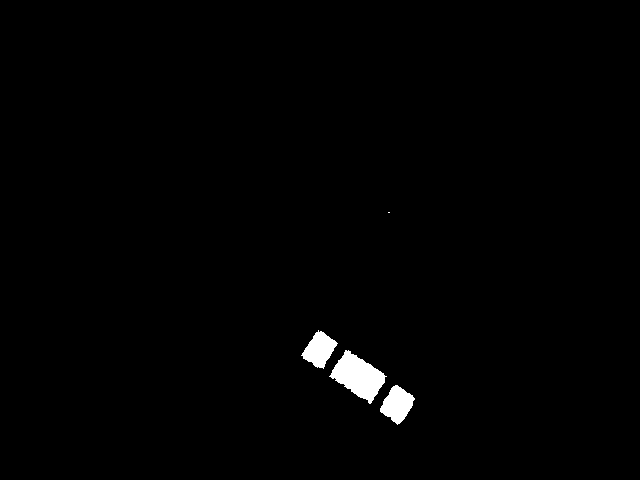
\includegraphics[width=\textwidth]{imaxes/IMPLEMENTACION/meta_a_mascara.png}
%        \caption{Máscara del color de la meta}
%        \label{fig:deteccion-meta-a}
%    \end{subfigure}
%    \hfill
%    \begin{subfigure}[b]{0.32\textwidth}
%        \centering
%        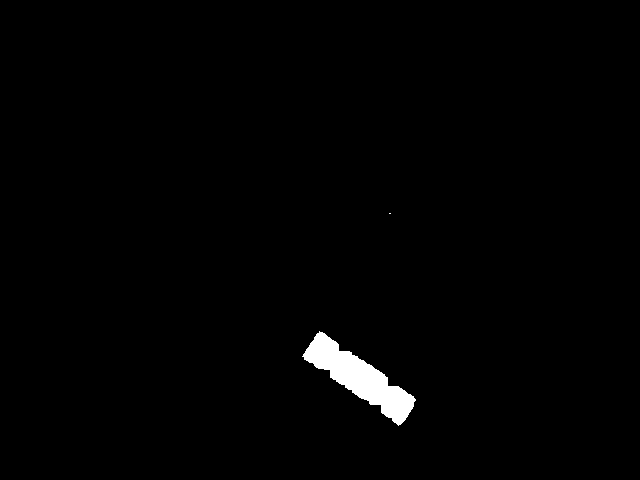
\includegraphics[width=\textwidth]{imaxes/IMPLEMENTACION/meta_b_cierre.png}
%        \caption{Tras el cierre morfológico}
%        \label{fig:deteccion-meta-b}
%    \end{subfigure}
%    \hfill
%    \begin{subfigure}[b]{0.32\textwidth}
%        \centering
%        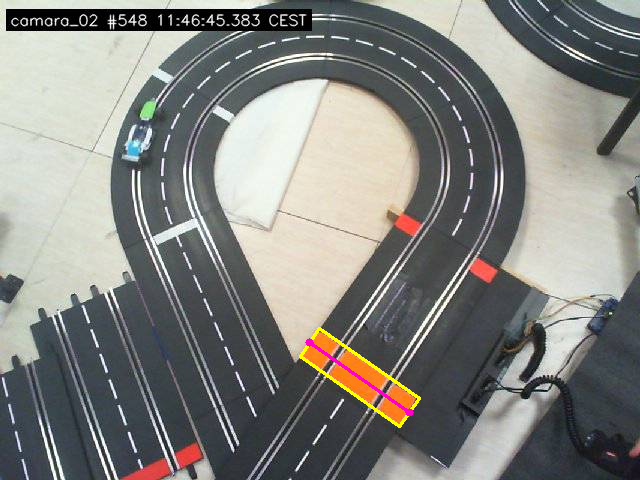
\includegraphics[width=\textwidth]{imaxes/IMPLEMENTACION/meta_c_segmento.png}
%        \caption{Rectángulo y segmento}
%        \label{fig:deteccion-meta-c}
%    \end{subfigure}
%    \caption{Detección de la línea de meta en la cámara~2. Los raíles parten la etiqueta en tres trozos que el cierre morfológico vuelve a unir; sobre la región resultante se ajusta el rectángulo de área mínima, rotado, y los puntos medios de sus lados cortos dan el segmento de meta.}
%    \label{fig:deteccion-meta}
%\end{figure}
%
%Cada nodo la busca al arrancar y, si no la ve, no publica línea de meta alguna. Por lo que en un despliegue multicámara solo lo hace la que observa la linea y generando el mensaje correspondiente (cuadro~\ref{tab:mensajes}). No hay, por tanto, una cámara de meta designada de antemano por el usuario.
%
%\subsection{Modo de depuración}
%\label{subsec:modo-depuracion}
%
%El nodo ofrece un modo de depuración, desactivado por defecto y activable en caliente o desde el fichero de parametros \ref{subsec:params-yaml}. En caso de que el flag este activado se conserva una copia del fotograma procesado sobre el cual se dibujan los rectángulos delimitadores de las pegatinas y una cruceta sobre cada centroide, y en una esquina su se pone el identificador del nodo, el número de fotograma y la hora de captura. El resultado se publica como \emph{vista de la cámara} (sección~\ref{subsec:mensajes-propios}), que es lo que permite seguir cada cámara en directo y lo que graba el sistema de visualización.
%
%\section{Nodo de control de carril}
%\label{sec:control-rail}
%
%El nodo controlador, uno por raíl según la sección~\ref{sec:arquitectura}, se divide como el de captura en dos componentes: el nodo de ROS~2, que gestiona la comunicación, los modos de funcionamiento y la detección del paso por meta, y un objeto que encapsula el algoritmo de velocidad, cuya implementación se detalla en la sección~\ref{sec:implementacion-algoritmo}.
%
%\subsection{Construcción de la trayectoria base}
%\label{subsec:control-modos}
%
%El nodo implementa los dos modos descritos en la sección~\ref{sec:modos_funcionamiento}, y su comportamiento cambia por completo de uno a otro.
%
%Durante la calibración el controlador acumula la posición de la pegatina delantera en un diccionario indexado por cámara: cada nodo de captura del que recibe mensajes tiene su propia lista de puntos y en ningún momento se construye una lista única con el circuito completo. Lo que delimita la acumulación es el paso por meta. Los puntos se recogen entre el primer cruce y el segundo, de modo que cada trayectoria base es una única vuelta que empieza en la meta; todo lo anterior, colocar el coche, arrancarlo y las vueltas que dé mientras se levanta el sistema, se descarta. El nodo sabe por sí solo cuándo terminar, porque es él quien detecta el paso por meta de su coche (sección~\ref{subsec:control-meta}).
%
%Al cerrarse la vuelta el controlador lo notifica en su \emph{topic} de calibración, filtra cada lista descartando los puntos que queden a menos de un umbral configurable del último aceptado, crea una instancia del algoritmo por cada cámara del diccionario, le inyecta su trayectoria y guarda una copia en la caché de la sección~\ref{subsec:cache-calibracion}.
%	
%Que se cierre sola es un requisito de la arquitectura. En los trabajos previos la arrancaba y la daba por concluida una persona desde una interfaz gráfica: había que delimitar el coche con un rectángulo y marcar la meta a mano~\cite{tfgmario}, o seleccionar el vehículo, activar el modo de búsqueda y confirmar los valores obtenidos~\cite{tfgadrian}. Con los nodos repartidos entre varias máquinas y sin interfaz desde la que supervisarlos, la calibración tiene que delimitarse y terminarse con la información que ya circula por la red.
%
%En modo carrera el controlador deja de acumular puntos y pasa a enrutar. Cada mensaje de posición de su coche se entrega a la instancia del algoritmo de la cámara que lo originó, identificada por el campo \texttt{camara\_id} del mensaje (sección~\ref{subsec:mensajes-propios}). La instancia devuelve el valor de PWM que hay que aplicar, que el controlador publica en su \emph{topic} de consigna, o bien la indicación de descartar el fotograma, en cuyo caso se mantiene el último valor válido. El funcionamiento interno del algoritmo se detalla en la sección~\ref{sec:implementacion-algoritmo}.
%
%Si se ordena volver al modo calibración, se descartan las trayectorias y las instancias y el proceso empieza de cero.
%
%\subsection{Control automático y control manual}
%\label{subsec:control-automatico-manual}
%
%Cerrada la calibración, el controlador entra en modo carrera y pasa de acumular puntos a enrutar posiciones. Es la pieza del sistema que aplica el algoritmo de velocidad, y cómo lo hace depende del indicador \texttt{modo\_manual} del coche, que se declara en el fichero de parámetros (sección~\ref{subsec:params-yaml}) y determina desde qué fichero de lanzamiento se levanta el nodo (sección~\ref{subsec:launch-files}).
%
%En control automático, cada mensaje de posición de su coche se entrega a la instancia del algoritmo de la cámara que lo originó, identificada por el campo \texttt{camara\_id} del mensaje (sección~\ref{subsec:mensajes-propios}). La instancia devuelve el valor de PWM que hay que aplicar, que el controlador publica en su \emph{topic} de consigna para que lo recoja el nodo puente, o bien la indicación de descartar el fotograma, en cuyo caso se mantiene el último valor válido. El controlador no decide nada por su cuenta: toda la lógica de control reside en el algoritmo, cuya implementación se detalla en la sección~\ref{sec:implementacion-algoritmo}.
%
%En control manual conduce una persona con el mando y el controlador no publica consigna alguna, de modo que el nodo puente nunca toca ese carril (sección~\ref{subsec:actuacion-topics}). El nodo hace por lo demás el mismo trabajo: calibra, sigue recibiendo posiciones, cuenta las vueltas de su coche y publica su telemetría. Sirve para registrar una carrera conducida por una persona con el mismo formato de datos que una automática, de manera que ambas puedan compararse después con la herramienta de análisis (sección~\ref{subsec:visualizacion-analisis}).
%
%Una carrera mixta, con coches de los dos tipos, se consigue levantando a la vez los dos ficheros de lanzamiento, tal como se describe en la sección~\ref{subsec:launch-files}.
%
%\subsection{Detección del paso por meta y medición de tiempos}
%\label{subsec:control-meta}
%
%El controlador cuenta las vueltas de su coche y mide su duración, que es lo que cierra el ciclo de aprendizaje del algoritmo (sección~\ref{subsec:algoritmo-aprendizaje}).
%
%El mecanismo se hereda del trabajo de Mario López~\cite{tfgmario} y solo se aplica a los mensajes de la cámara que publicó la línea de meta. Para cada posición se calcula el producto vectorial entre el vector que recorre el segmento de meta y el que va de uno de sus extremos a la pegatina delantera. Su signo indica de qué lado de la recta que contiene al segmento está el coche, de modo que un cambio de signo entre dos fotogramas consecutivos significa que lo ha cruzado.
%
%\begin{figure}[tbp]
%    \centering
%    \begin{subfigure}[b]{0.48\textwidth}
%        \centering
%        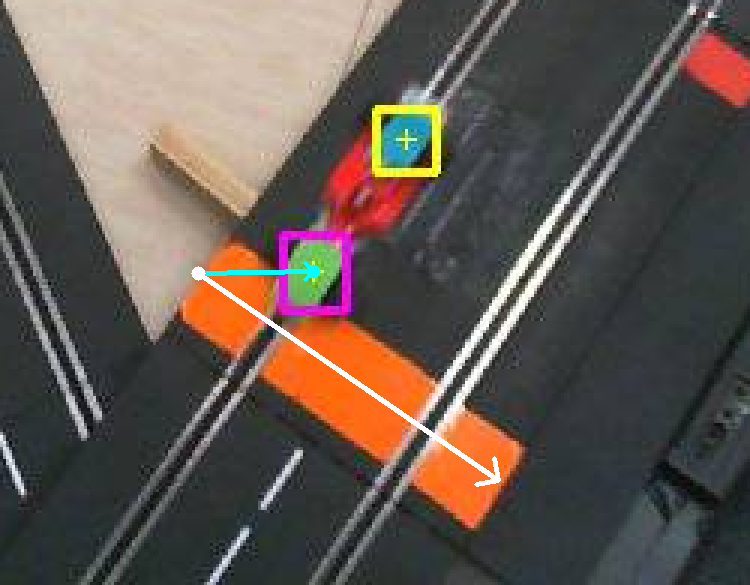
\includegraphics[width=\textwidth]{imaxes/IMPLEMENTACION/meta_vector_a_antes.png}
%        \caption{Antes de cruzar}
%        \label{fig:producto-vectorial-a}
%    \end{subfigure}
%    \hfill
%    \begin{subfigure}[b]{0.48\textwidth}
%        \centering
%        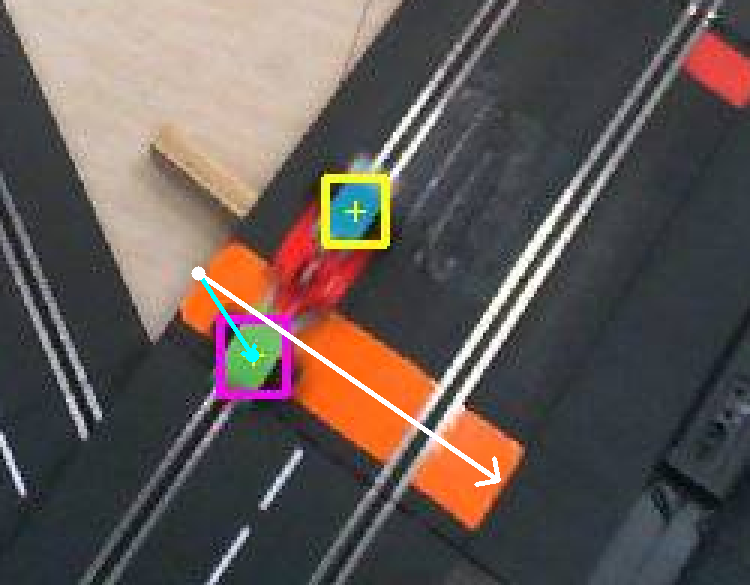
\includegraphics[width=\textwidth]{imaxes/IMPLEMENTACION/meta_vector_b_despues.png}
%        \caption{Después de cruzar}
%        \label{fig:producto-vectorial-b}
%    \end{subfigure}
%    \caption{Ejemplo de cómo se detecta el cruce por meta}
%    \label{fig:producto-vectorial}
%\end{figure}
%
%Detectado el cambio de lado, el instante del cruce se aproxima interpolando entre los dos fotogramas implicados, el anterior a la meta y el posterior. La fracción del intervalo recorrida hasta tocar la recta es el cociente entre la distancia del fotograma anterior y la suma de ambas distancias. Sin interpolar, tomar la marca del fotograma que detecta el cruce introduciría un error de hasta un período de captura en cada vuelta.
%
%Los instantes que se interpolan son las marcas de tiempo que la cámara pone al capturar el fotograma, no el momento en que llega el mensaje, por la razón expuesta en la sección~\ref{subsec:qos}. Así no hace falta sincronizar los relojes de las máquinas, porque el tiempo por vuelta se calcula siempre contra la misma referencia temporal, la de la cámara. En cada cruce el controlador publica el tiempo y el número de vuelta en su \emph{topic} de telemetría y notifica el evento a todas las instancias del algoritmo, indicando si la vuelta fue limpia.
%
%El método arrastra una limitación que ya señalaba Mario López~\cite{tfgmario}: el signo se calcula contra la recta infinita que contiene al segmento y, como el circuito es cerrado, esa recta vuelve a cortar la pista en otro punto, donde el signo cambia igual. Él lo evitaba calculando el producto solo con el coche a menos de vez y media su longitud de un extremo de la meta; aquí el cambio de signo se ignora mientras la distancia de la pegatina a la meta supere un umbral configurable.
%
%% TODO: figura de la recta de meta prolongada cortando el circuito en un segundo punto (equivalente a la figura 5.9 de la memoria de Mario López)
%
%Este método sustituye al del trabajo de Adrián Rego~\cite{tfgadrian}, que fue el primero que se implementó. Con el coche muy lento o detenido sobre la línea de meta llegaba a fallar la cuenta, de modo que se cambió por el del cambio de signo, que no depende de la velocidad a la que se cruce.
%
%\section{Implementación del algoritmo de velocidad}
%\label{sec:implementacion-algoritmo}
%
%Esta sección detalla cómo se implementa el algoritmo cuyo diseño se describió en la sección~\ref{sec:algoritmo-arquitectura}. Su entrada es una posición del coche sobre la imagen de una cámara y su salida el valor de PWM que hay que aplicar al carril. Durante este proceso se usa la trayectoria base aprendida durante la calibración, se detectan derrapes y se aplican las dos políticas de ajuste.
%
%\subsection{Instancias por cámara}
%\label{subsec:algoritmo-instancias}
%
%El algoritmo no trabaja sobre el circuito completo, sino sobre la porción que observa una cámara. El controlador mantiene un diccionario indexado por identificador de cámara (sección~\ref{subsec:control-modos}), que guarda la lista de puntos acumulados de esa cámara durante la calibración. Al cerrarse la vuelta, cada lista da lugar a una instancia independiente del algoritmo, con su propia cadena de celdas, sus propias zonas y su propio perfil de PWM.
%
%La consecuencia es que no existe una trayectoria global del circuito. Cada trayectoria vive en las coordenadas de imagen de su cámara y ninguna instancia conoce nada de las demás, no hay fusión de trayectorias y  tampoco un sistema de referencia común. El único punto del proyecto en el que todas se llevan a un plano común es la herramienta de análisis en diferido (sección~\ref{subsec:visualizacion-analisis}), que queda fuera del lazo de control. Hacerlo de esta forma es porque permite facilita el trabajo y reduce el esfuerzo que hay que realizar.
%
%La visión de conjunto la aporta el controlador, no el algoritmo. Es el controlador quien enruta cada posición a la instancia que le corresponde, quien decide qué cámara está activa en cada momento, quien cierra un derrape en una cámara y abre su continuación en la siguiente, quien propaga hacia atrás las reducciones que no caben en una porción y quien determina si una vuelta ha sido limpia en todo el trazado. Esos mecanismos se describen en la sección~\ref{subsec:algoritmo-coordinacion}.
%
%\subsection{Construcción de la cadena de celdas}
%\label{subsec:algoritmo-celdas}
%
%La trayectoria base de la sección~\ref{subsec:trayectoria-base} se transforma en una sucesión ordenada de celdas. Al terminar la calibración cada instancia recibe la lista de puntos de su cámara y la remuestrea, porque los puntos crudos no están repartidos de forma uniforme, su separación depende de la velocidad que llevase el coche al grabarlos y de si todas las posiciones enviadas por la camara llegaron al controlador. Se recorre esta trayectoria colocando una celda cada cierta distancia fija e interpolando entre puntos consecutivos, de modo que las celdas quedan equiespaciadas sobre la trayectoria real que sigue el coche en el circuito, independientemente de como cayeran los puntos originales. 
%
%Los saltos entre puntos consecutivos que superan un umbral reciben otro tratamiento. Corresponden a tramos que la cámara no ve, porque un puente o otro elemento tapan la pista, y no tiene sentido interpolar dentro de ellos. En su lugar se crea una única \emph{celda gigante} que registra la longitud real del hueco. Dentro de ella no puede localizarse el coche ni detectarse derrapes, pero se trata todo con un mismo valor de PWM.
%
%\subsection{Localización del coche sobre la trayectoria}
%\label{subsec:algoritmo-localizacion}
%
%Para poder realizar el control es necesario saber donde están las dos pegatinas del coche, tanto la delantera como la trasera, con respecto a la trayectoria base, (sección~\ref{subsec:trayectoria-base}). Razón por la cual, para cada una se obtiene la celda más cerca y su distancia a ella.
%
%Después cada una tiene un uso distinto. La distancia de la delantera es una comprobación realizada para comprobar que el coche sigue el recorrido esperado, si supera un umbral se considera que la detección no es válida y el fotograma se descarta sin llegar a calcular un PWM nuevo. La distancia de la trasera es la señal con la que se detectan los derrapes, como se detalla en la sección~\ref{subsec:algoritmo-derrapes}.
%
%El procedimiento es el mismo para ambas. Primero se busca la celda cuyo punto está más próximo al centroide de la pegatina. Después se proyecta ese centroide sobre los dos segmentos que unen la celda escogida con su anterior y su posterior, y se conserva la menor de las dos distancias. La proyección hace falta porque medir contra la celda daría una distancia que no es precisa, en cambio contra los segmentos se obtiene la distancia perpendicular a la trayectoria.
%
%La proyección solo puede hacerse entre celdas consecutivas, porque a través de una celda gigante no hay trayectoria conocida sobre la que proyectar. .
%
%\subsection{Detección de derrapes}
%\label{subsec:algoritmo-derrapes}
%
%La sección~\ref{subsec:derrape-arquitectura} exige que exista una señal capaz de indicar en qué punto del circuito el coche ha perdido el control, es decir, derrapado. La señal escogida aquí es la distancia perpendicular de la pegatina trasera a la trayectoria. Cuando la parte trasera del coche se abre, esa distancia crece, mientras la delantera sigue marcando la posición sobre el trazado.
%
%La detección se implementa como una máquina de estados que se alimenta en cada fotograma con la celda y la distancia perpendicular de la pegatina trasera. Cuando la distancia supera el umbral de derrape se abre uno y se anota la celda inicial, mientras se mantenga por encima, el derrape se prolonga actualizando su celda final; cuando vuelve a caer por debajo, se cierra. No se abren derrapes junto a los extremos de la cadena ni junto a las celdas gigantes, donde la medida no es fiable.
%
%La figura~\ref{fig:secuencia-derrape} ejemplifica un caso donde se puede ver el proceso real de derrape del coche. Con el coche alineado la pegatina trasera va sobre el carril y su distancia a la trayectoria es casi nula; al abrirse la parte trasera la distancia perpendicular del centroide de la pegatina a la trayectoria crece hasta superar el umbral, que es lo que abre el derrape, se puede ver en la figura~\ref{fig:derrape-trazas-b}. En el instante más violento el coche queda atravesado y ninguna de las dos pegatinas se detecta, situación que resuelve la readquisición de la sección~\ref{subsec:readquisicion}.
%
%\begin{figure}[tbp]
%    \centering
%    \begin{subfigure}[b]{0.48\textwidth}
%        \centering
%        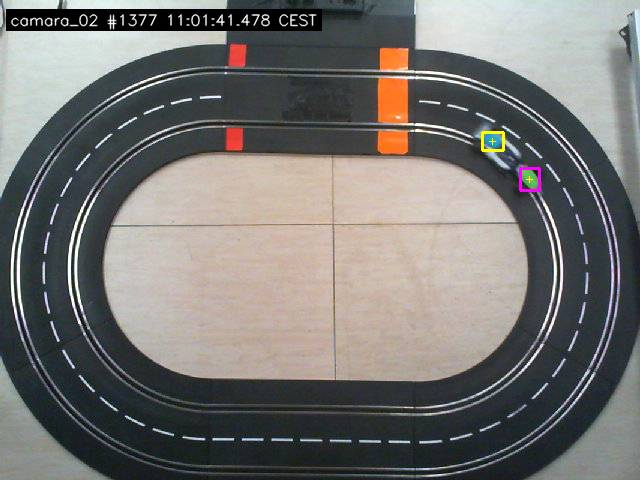
\includegraphics[width=\textwidth]{imaxes/IMPLEMENTACION/derrape_seq_a_antes.png}
%        \caption{Coche alineado con el carril}
%        \label{fig:secuencia-derrape-a}
%    \end{subfigure}
%    \hfill
%    \begin{subfigure}[b]{0.48\textwidth}
%        \centering
%        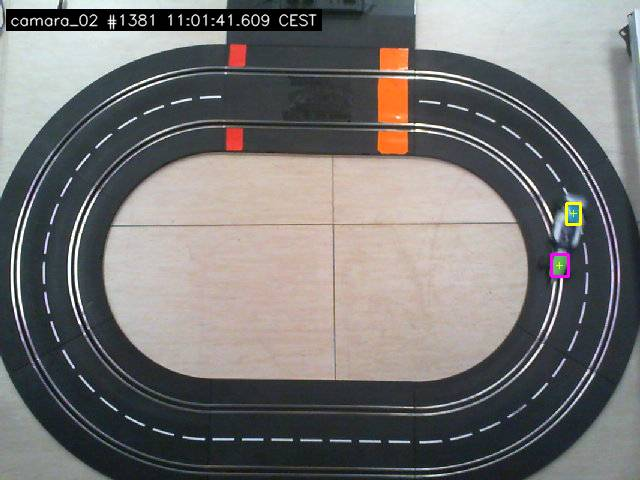
\includegraphics[width=\textwidth]{imaxes/IMPLEMENTACION/derrape_seq_b_inicio.png}
%        \caption{La parte trasera empieza a abrirse}
%        \label{fig:secuencia-derrape-b}
%    \end{subfigure}
%
%    \vspace{0.7em}
%    \begin{subfigure}[b]{0.48\textwidth}
%        \centering
%        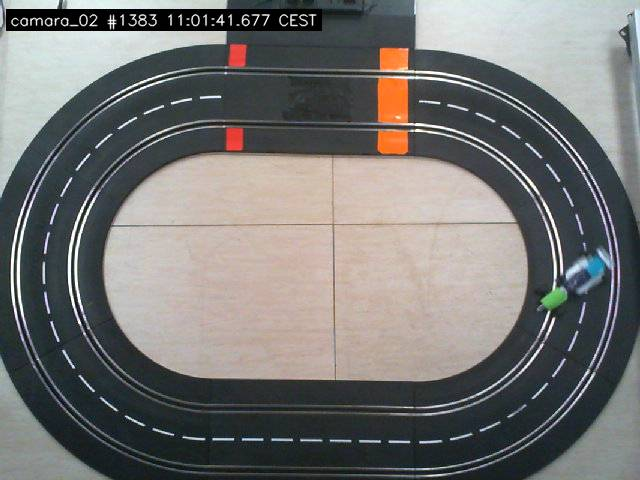
\includegraphics[width=\textwidth]{imaxes/IMPLEMENTACION/derrape_seq_c_completo.png}
%        \caption{Derrape completo, sin detección}
%        \label{fig:secuencia-derrape-c}
%    \end{subfigure}
%    \hfill
%    \begin{subfigure}[b]{0.48\textwidth}
%        \centering
%        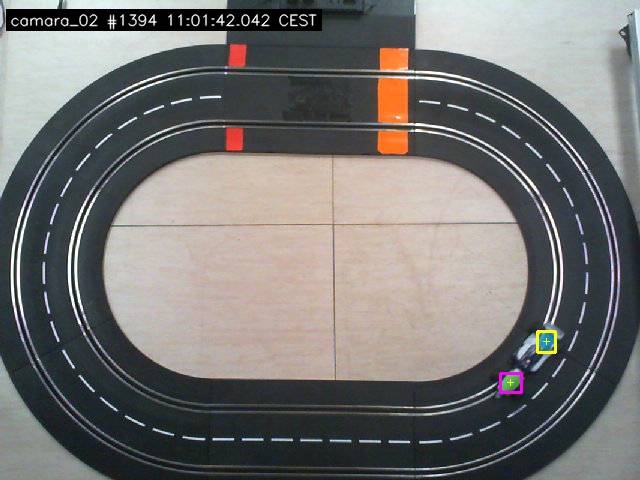
\includegraphics[width=\textwidth]{imaxes/IMPLEMENTACION/derrape_seq_d_recuperado.png}
%        \caption{Seguimiento readquirido}
%        \label{fig:secuencia-derrape-d}
%    \end{subfigure}
%    \caption{Ejemplo de proceso de derrape en el circuito en forma de ovalo}
%    \label{fig:secuencia-derrape}
%\end{figure}
%
%\subsection{Castigo de zonas y ciclo de aprendizaje}
%\label{subsec:algoritmo-aprendizaje}
%
%Las zonas y las dos políticas que actúan sobre ellas se definieron en la sección~\ref{subsec:zonas-politicas}. Cada instancia mantiene la partición de su cadena de celdas en zonas, aplica la política de castigo al cerrarse un derrape y la de mejora al completarse una vuelta.
%
%Cada derrape cerrado desencadena el castigo. El intervalo de celdas del derrape se extiende hacia atrás una distancia fija en píxeles, que es el tramo de anticipación que exige la arquitectura, y el resultado se convierte en una zona de derrape. Su PWM se fija en el mínimo de los de las zonas que cubría el intervalo, menos una reducción fija (de dos unidades), con el parámetro \texttt{minimum\_speed} (sección~\ref{subsec:params-yaml}) como suelo.
%
%Si el derrape cae dentro o junto a una zona de derrape ya existente, ambas se fusionan. El intervalo resultante es la unión de los dos y el PWM, el mínimo de ambos menos la reducción. En ese caso el retroceso añadido es menor que el de una zona nueva, porque la zona existente ya aplicó el suyo al crearse. Si cada reincidencia retrocediera de nuevo la distancia completa, las zonas protegidas acabarían cubriendo el circuito entero y el perfil no volvería a subir en ningún tramo. Las celdas gigantes alcanzadas por un derrape o por su retroceso se castigan como una unidad, ya que dentro del hueco no hay precisión que permita distinguir una parte de otra.
%
%La política de mejora se dispara con el paso por meta. El controlador comprueba si durante la vuelta hubo algún derrape en alguna de las cámaras y comunica el resultado a todas las instancias. Cada zona sin derrape incrementa su PWM en una unidad, con \texttt{maximum\_speed} como techo. Quedan fuera las zonas que registraron un derrape en las últimas vueltas, que permanecen protegidas durante un número configurable de vueltas antes de poder volver a subir.
%
%Las figuras~\ref{fig:derrape-trazas} y~\ref{fig:derrape-dist} recorren el ciclo completo sobre tres vueltas consecutivas de una sesión, con las gráficas de la herramienta de análisis (sección~\ref{subsec:visualizacion-analisis}). En la vuelta~21 la trasera va pegada a la trayectoria base y la distancia nunca se acerca al umbral, de modo que el PWM se mantiene igual en todo el recorrido y solamente hay una zona. En la~22 la trasera se abre en la curva y la distancia lo supera durante diez fotogramas, lo que cierra un derrape y castiga la zona. En la~23 el perfil ya trae el PWM rebajado en ese tramo.
%
%\begin{figure}[tbp]
%    \centering
%    \begin{subfigure}[b]{0.48\textwidth}
%        \centering
%        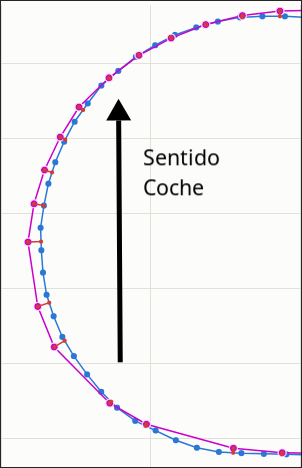
\includegraphics[width=\textwidth]{imaxes/IMPLEMENTACION/derrape_traza_v21.png}
%        \caption{Vuelta 21, limpia}
%        \label{fig:derrape-trazas-a}
%    \end{subfigure}
%    \hfill
%    \begin{subfigure}[b]{0.48\textwidth}
%        \centering
%        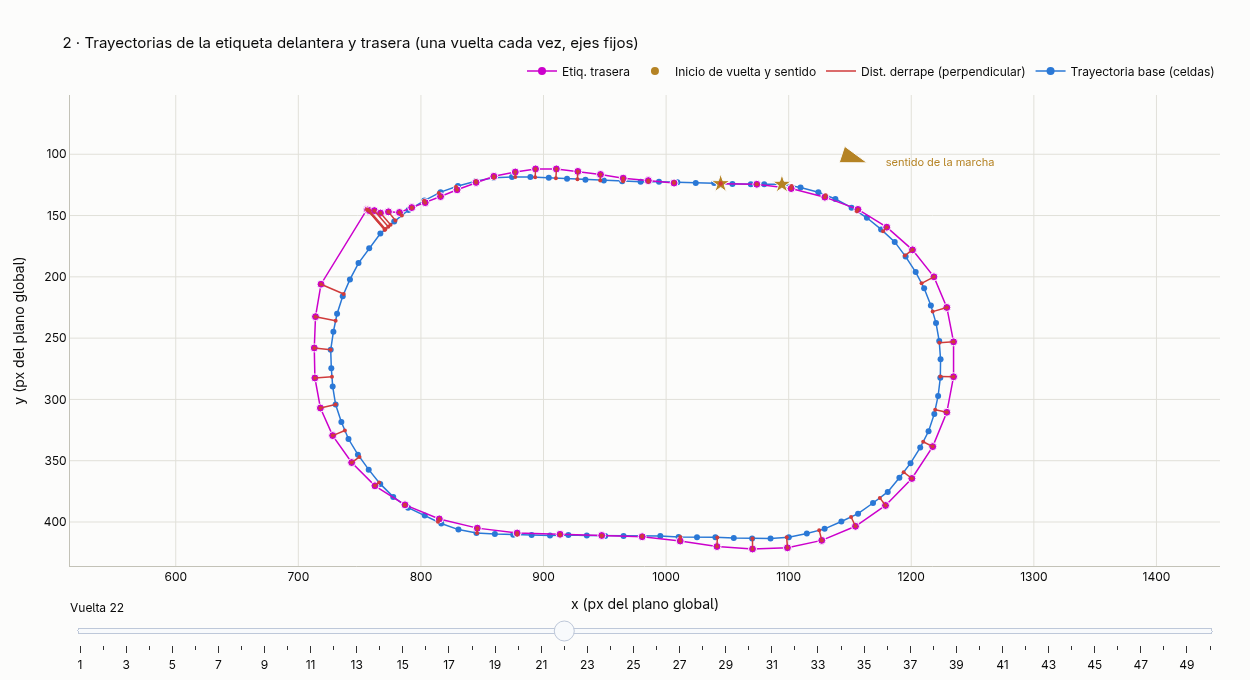
\includegraphics[width=\textwidth]{imaxes/IMPLEMENTACION/derrape_traza_v22.png}
%        \caption{Vuelta 22, con derrape}
%        \label{fig:derrape-trazas-b}
%    \end{subfigure}
%
%    \vspace{0.7em}
%    \begin{subfigure}[b]{0.48\textwidth}
%        \centering
%        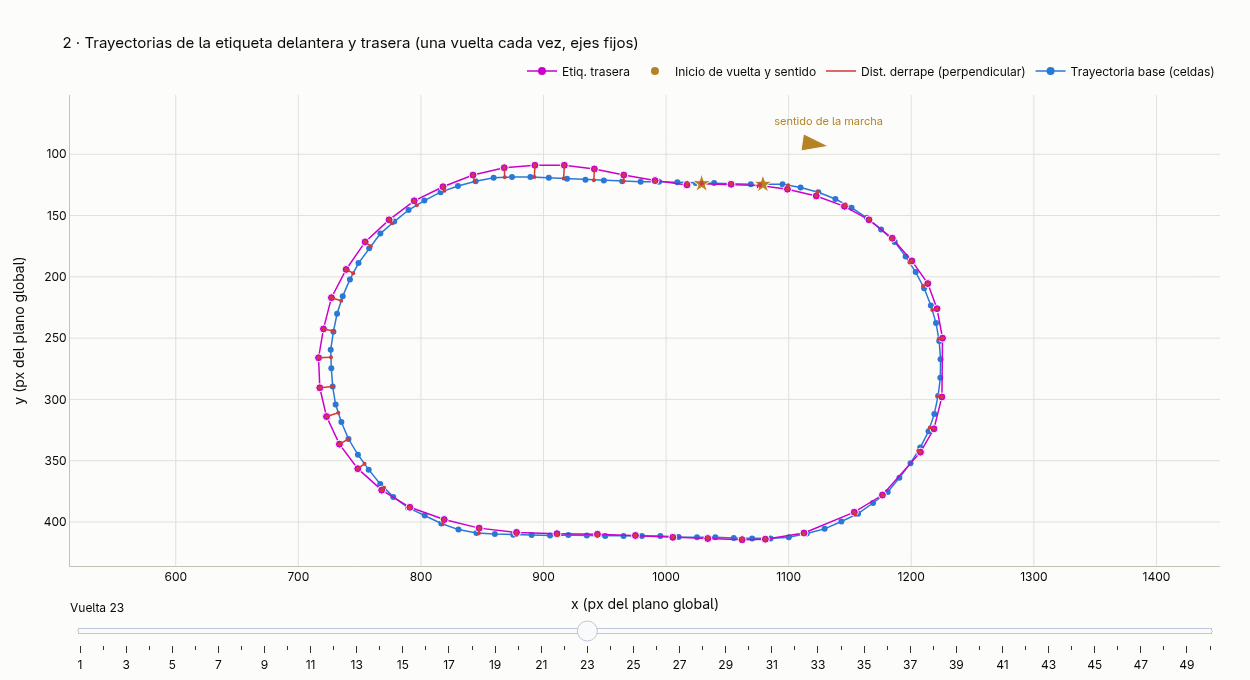
\includegraphics[width=\textwidth]{imaxes/IMPLEMENTACION/derrape_traza_v23.png}
%        \caption{Vuelta 23, ya castigada}
%        \label{fig:derrape-trazas-c}
%    \end{subfigure}
%    \caption{Recorrido de la pegatina trasera (magenta) frente a la trayectoria base (azul) en tres vueltas consecutivas. Los segmentos rojos son la distancia perpendicular que mide el algoritmo}
%    \label{fig:derrape-trazas}
%\end{figure}
%
%\begin{figure}[p]
%    \centering
%    \begin{subfigure}[b]{0.85\textwidth}
%        \centering
%        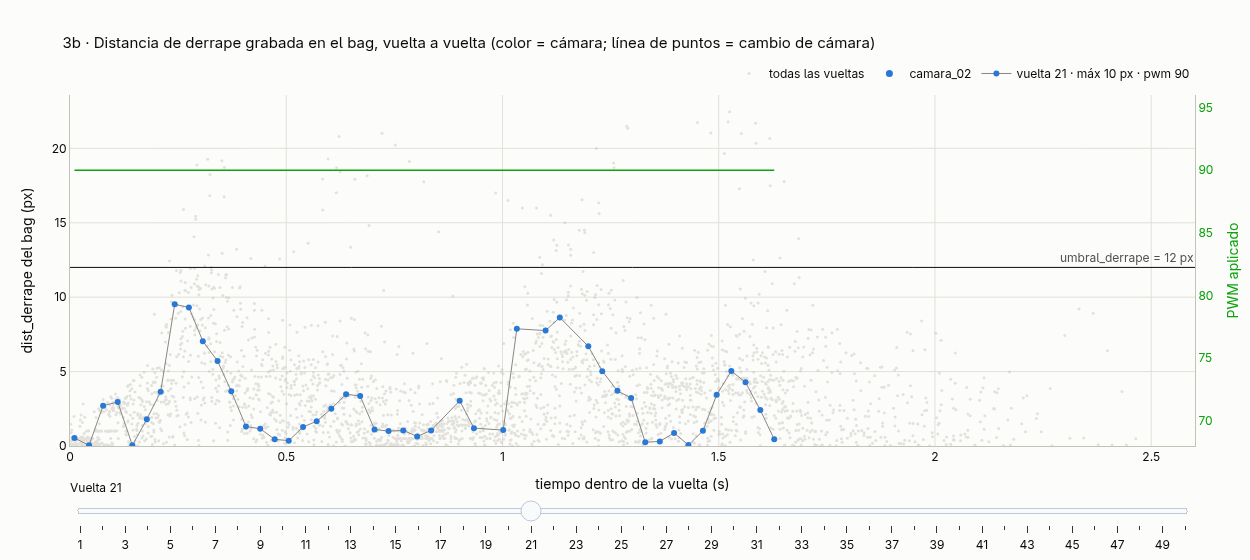
\includegraphics[width=\textwidth]{imaxes/IMPLEMENTACION/derrape_dist_v21.png}
%        \caption{Vuelta 21}
%        \label{fig:derrape-dist-a}
%    \end{subfigure}
%
%    \vspace{0.5em}
%    \begin{subfigure}[b]{0.85\textwidth}
%        \centering
%        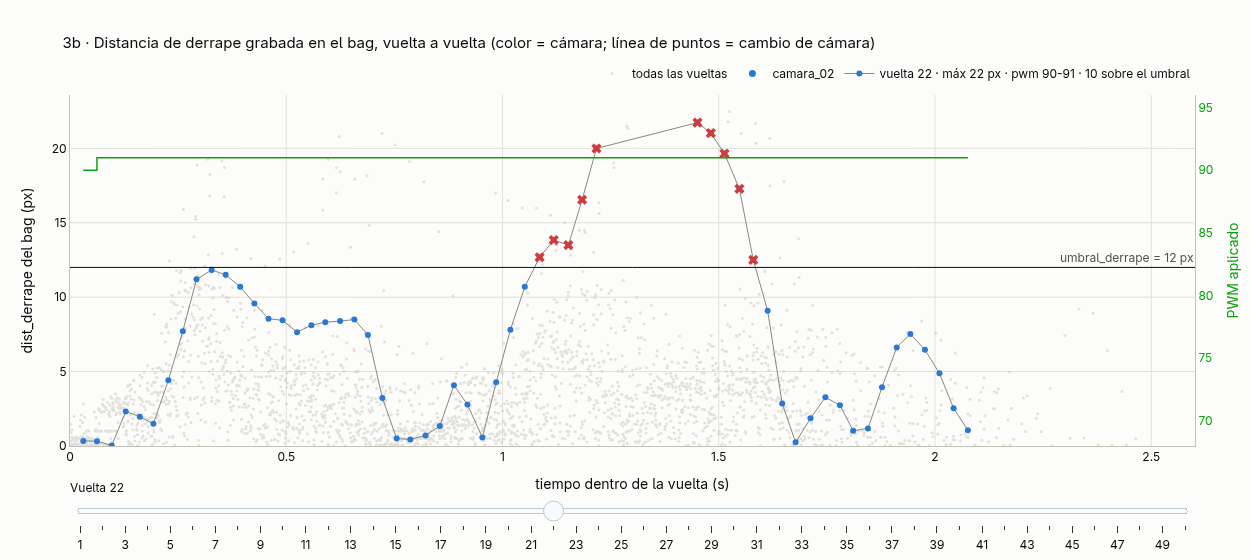
\includegraphics[width=\textwidth]{imaxes/IMPLEMENTACION/derrape_dist_v22.png}
%        \caption{Vuelta 22}
%        \label{fig:derrape-dist-b}
%    \end{subfigure}
%
%    \vspace{0.5em}
%    \begin{subfigure}[b]{0.85\textwidth}
%        \centering
%        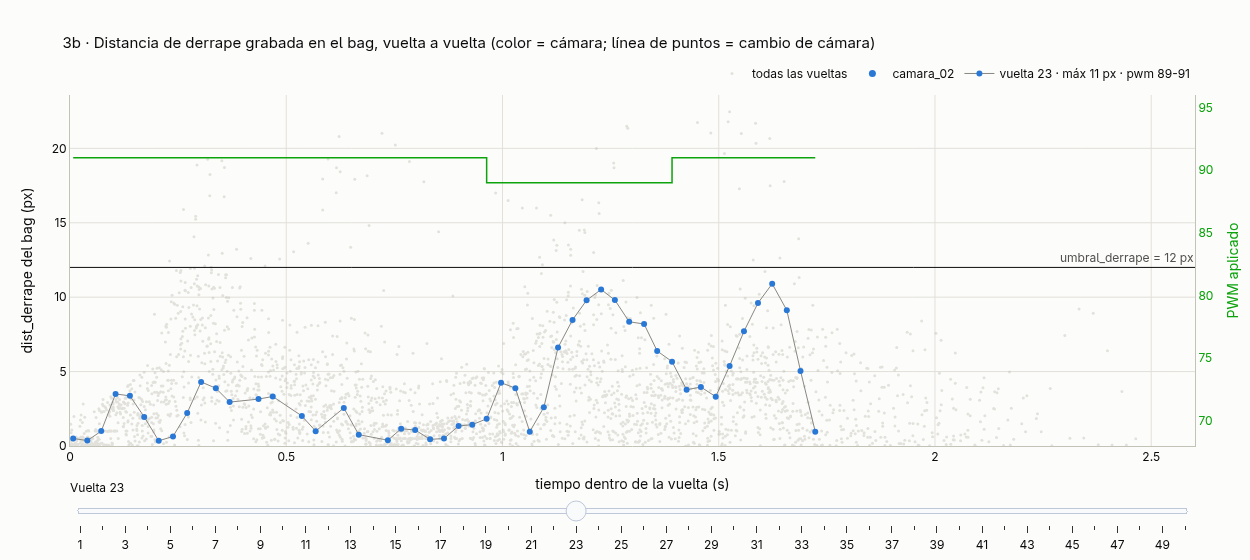
\includegraphics[width=\textwidth]{imaxes/IMPLEMENTACION/derrape_dist_v23.png}
%        \caption{Vuelta 23}
%        \label{fig:derrape-dist-c}
%    \end{subfigure}
%    \caption{Distancia de la pegatina trasera a lo largo de cada vuelta (eje izquierdo) frente al PWM aplicado (línea verde, eje derecho). Las aspas rojas marcan las muestras que superan el umbral y abren el derrape. El escalón verde de la vuelta~23 es la zona creada por el castigo de la anterior.}
%    \label{fig:derrape-dist}
%\end{figure}
%
%\subsection{Coordinación entre cámaras}
%\label{subsec:algoritmo-coordinacion}
%
%Cada instancia conoce solo su porción del circuito (sección~\ref{subsec:algoritmo-instancias}), de modo que hay tres situaciones que ninguna puede resolver por sí sola y que asume el controlador.
%
%La primera es la transición del coche entre cámaras. Cuando dos campos de visión se solapan, ambas publican posiciones intercaladas del mismo coche, así que la cámara activa se mantiene mientras siga entregando fotogramas válidos y solo se cambia a otra cuando deja de hacerlo durante un breve intervalo y esa otra sí está entregando. En cada cambio el controlador notifica la pérdida de visión a la cámara saliente. Como el coche recorre siempre el circuito en el mismo sentido, tras una vuelta completa ese registro contiene el orden secuencial de las cámaras, aprendido en carrera y sin configuración manual.
%
%La segunda es el derrape repartido entre dos cámaras. Al recibir la notificación de pérdida de visión, la instancia saliente cierra el derrape que tuviera abierto y la entrante recibe la orden de abrir uno nuevo, en caso de que el derrape siguiera activo. La zona de derrape se extiende así entre cámaras y el derrape se detecta aunque el corte entre cámaras caiga en mitad de una curva.
%
%La tercera es la propagación de reducciones. Ocurre cuando un derrape se produce cerca del inicio de la porción visible de una cámara, algo habitual si una curva queda repartida entre dos cámaras. El retroceso del castigo se sale por el inicio antes de agotarse y los píxeles restantes corresponden a un tramo de otra cámara. La instancia anota ese sobrante como reducción pendiente; el controlador la recoge tras procesar cada posición y, según el orden aprendido, ordena a la cámara precedente que la aplique al final de su trayectoria, creando o ampliando allí la zona de derrape. Esa reducción externa no incrementa el contador de derrapes de quien la recibe, porque ese derrape ya lo contabilizó la cámara que lo observó, pero la zona queda protegida igual. Si tampoco llegara la trayectoria de la camara anterior, el sobrante volvería a quedar pendiente y se propagaría en poco hacia atrás hasta terminarse.
%
%\section{Nodo de actuación}
%\label{sec:sistema-actuacion}
%
%El nodo de actuación envía hacia el Arduino los valores de PWM calculados por los controladores. Está formado por dos componentes, en primer lugar el nodo puente de ROS~2, que centraliza la recepción de las consignas de todos los controladores, y en segundo lugar el subsistema hardware, compuesto por la placa Arduino y el módulo controlador de motores (L293D).
%
%\subsection{Tratamiento de las consignas recibidas}
%\label{subsec:actuacion-topics}
%
%El nodo puente es un nodo puramente consumidor, no publica nada, se limita a suscribirse a los \emph{topics} en los que cada controlador anuncia el PWM de su carril. Las suscripciones se generan dinámicamente, una por cada coche declarado en la lista de configuración, \ref{subsec:params-yaml}.
%
%De cada mensaje extrae el identificador del carril y su valor de PWM, y le aplica dos comprobaciones antes de mandarlo al puerto serie. La primera es un filtro de repetición, el nodo guarda el último valor enviado a cada carril y descarta el mensaje si coincide con él. Como los controladores publican una consigna por cada posición recibida y el PWM se mantiene estable durante tramos enteros del circuito, este filtro reduce drásticamente el tráfico sobre el puerto. La segunda es una validación del rango admitido por el hardware, entre 0 y 255, como última barrera frente a consignas mal formadas.
%
%El nodo se suscribe también al \emph{topic} de calibración de cada coche que este configurado para control automatico. Durante esa fase es él quien aplica al carril un valor de potencia que permite tener una velocidad de calibración constante, porque los controladores todavía no publican consigna alguna. En cuanto un coche cierra su vuelta se pasa a aplicar el valor que publica el controlador. Los carriles de los coches marcados como manuales no se tocan en ningún momento.
%
%\subsection{Comunicación con el Arduino}
%\label{subsec:actuacion-interfaz}
%
%La comunicación con la placa se encapsula, como en el trabajo de Adrián Rego~\cite{tfgadrian}, en una clase independiente que forma parte del nodo y que abstrae, la complejidad de la comunicación con el puerto serie, en operaciones de alto nivel: fijar la velocidad de un carril, la de ambos o detenerlos. Al inicializarse enumera los puertos disponibles y, si el configurado no está, toma el primer dispositivo compatible que encuentre; después espera a que la placa termine de reiniciarse, vacía el búfer de entrada y detiene ambos carriles, de modo que el sistema arranca siempre desde un estado seguro.
%
%El protocolo es textual y mínimo. Cada orden es una línea de la forma \texttt{r<carril>:<valor>}, por ejemplo \texttt{r1:120}, donde el primer campo identifica el carril y el segundo el PWM a aplicar. El envío es bloqueante, tras escribir la orden la interfaz espera la confirmación de la placa (\texttt{OK}) y solo entonces da la operación por completada; si no llega dentro del tiempo límite, el envío se considera fallido. Aquí ese carácter bloqueante es lo que serializa el acceso.
%
%\subsection{Subsistema hardware}
%\label{subsec:actuacion-hardware}
%
%El subsistema hardware traduce las órdenes recibidas por el puerto serie en la tensión que se aplica sobre los raíles. El montaje es el del trabajo de Adrián Rego~\cite{tfgadrian} y se reutiliza sin cambios. La placa se conecta al ordenador por USB, que es a la vez el canal serie y la alimentación de los motores, y del módulo controlador parten hacia la pista una masa común y dos salidas de potencia, una por carril. Los componentes se describen en la sección~\ref{sec:tecnoloxias-hardware}.
%
%Sobre la placa corre un firmware sencillo, cargado con el IDE de Arduino, que configura los pines de salida PWM, lee el puerto serie a la espera de órdenes y, por cada línea recibida, aplica la señal sobre el pin del carril indicado y responde con la confirmación que la interfaz espera. El ciclo de trabajo del pin es proporcional al valor recibido: 0 corresponde a un ciclo nulo, con el carril detenido, y 255 al ciclo completo; de ahí sale el rango que valida el nodo puente.
%
%Lo que aporta este trabajo no es el montaje, sino su encaje en la arquitectura distribuida. En el trabajo previo la interfaz vivía dentro de una aplicación de escritorio que era también quien procesaba las imágenes y decidía las velocidades; aquí queda detrás del nodo puente el cual permite una comunicación y controla el acceso.
%
%\section{Sistema de visualización y análisis}
%\label{sec:sistema-visualizacion}
%
%El sistema de visualización se compone de dos herramientas independientes que solo se comunican a través de los ficheros que una genera y la otra consume. La de grabación se despliega junto al resto del sistema mientras la sesión está en marcha y almacena todos los mensajes que circulan por la red, en cambio, la de análisis coge la informacion en diferido. Se ejecuta si el usuario quiere al terminar y recibe como entrada el bag generado y los \emph{logs} de los algoritmos a partir de los cuales construye un \emph{dashboard} web que permite estudiar la carrera vuelta a vuelta (figura~\ref{fig:flujo-visualizacion}).
%
%\begin{figure}[H]
%    \centering
%    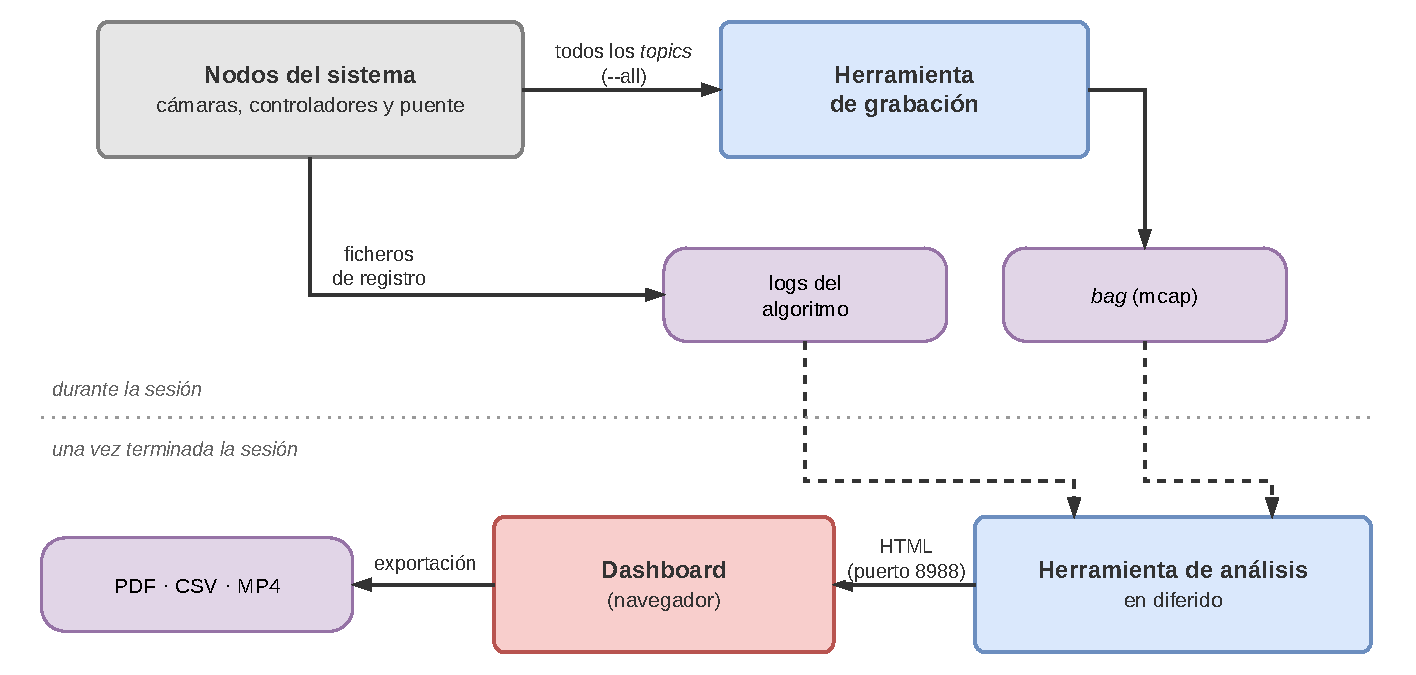
\includegraphics[width=\textwidth]{imaxes/IMPLEMENTACION/flujo_analisis_sistema.pdf}
%    \caption{Esquema que permite ver como es el flujo que se realiza dentro del sistema de analisis}
%    \label{fig:flujo-visualizacion}
%\end{figure}
%
%\subsection{Herramienta de grabación}
%\label{subsec:visualizacion-grabacion}
%
%La herramienta de grabación tiene como cometido capturar sin pérdidas todo el tráfico de la red durante una sesión y dejarlo en disco, sin procesar ni interpretar nada. Se construye sobre \emph{rosbag2} (sección~\ref{sec:ros2-rosbag}), empaquetada en un contenedor junto con las definiciones de los mensajes propios del proyecto, que hay que compilar dentro para que pueda interpretarlos.
%
%La herramienta soporta un descubrimiento dinamico lo que permite grabar sin conocer de antemano qué nodos van a estar presentes. Una primera versión trabajaba con una lista explícita de \emph{topics}, construida a partir del número de cámaras y coches configurados, y resultó una fuente constante de errores porque por cada \emph{topic} nuevo o renombrado había que acordarse de reflejarlo en ella. La versión definitiva graba la totalidad de los \emph{topics} y sondea periódicamente en busca de otros, suscribiéndose a los que van apareciendo, de modo que no impone ningún orden de arranque. La calidad de servicio se resuelve igual, en lugar de mantener un fichero que reprodujera las políticas del sistema, la herramienta adapta el perfil de cada suscripción al que ofrecen los publicadores que encuentra.
%
%Se escogio el formato \emph{mcap} porque lleva embebida la definición de cada mensaje lo que permite poder seguir analizando todos los bags aunque no dispongamos ya de la definion de los mensajes, esto es debido a que los mensajes del sistema fueron evolucionando conforme avanzaba el proyecto.
%
%\subsection{Herramienta de análisis en diferido}
%\label{subsec:visualizacion-analisis}
%
%La herramienta de análisis convierte los datos crudos de una sesión en un conjunto de gráficas. Combina dos fuentes: la grabación(\emph{bags}), de la que obtiene todo lo que se publicó en la red, y los ficheros de \emph{logs} que escribe el algoritmo, de los que obtiene su estado interno. La primera describe qué hizo el coche y los segundos explican por qué el sistema decidió lo que decidió, de modo que solo cruzando ambas se puede relacionar un comportamiento con la decisión que lo provocó.
%
%El resultado es un \emph{dashboard}, una página web autocontenida con gráficas interactivas que permiten desplazarse, ampliar una zona y consultar el valor de cada punto, organizada en las secciones numeradas que recoge el cuadro~\ref{tab:secciones-dashboard}. Como cada cámara trabaja en sus propias coordenadas de imagen, todas las gráficas espaciales se dibujan sobre un plano global común, aplicando a cada cámara una traslación fija. Desde el propio \emph{dashboard} pueden exportarse las gráficas en PDF, los datos en CSV y descargar un vídeo que combina las imágenes de todas las cámaras.
%
%También el análisis se ejecuta en un contenedor, que a diferencia del resto no forma parte del sistema desplegado. Se levanta bajo demanda indicándole qué sesión analizar, genera el \emph{dashboard}, lo sirve en un puerto accesible desde la máquina anfitriona y termina al pararlo. Necesita contenedor por la misma razón que la grabación, leer ficheros mcap exige tener disponibles las bibliotecas de ROS~2 y las definiciones de los mensajes.
%
%\begin{table}[htbp]
%\centering
%\resizebox{\textwidth}{!}{
%\begin{tabular}{|c|l|}
%\hline
%\rowcolor{ArqAzulClaro}
%\textbf{Sección} & \textbf{Contenido} \\
%\hline
%0 & Resumen de la sesión \\
%\hline
%1 & Valor del derrape en cada punto del recorrido (3D) \\
%\hline
%2 & Trayectorias de las etiquetas delantera y trasera \\
%\hline
%3 & Distancia de derrape de la etiqueta trasera \\
%\hline
%4 & Mapa del circuito con el PWM de cada celda \\
%\hline
%5 & Tiempos por vuelta \\
%\hline
%6 & Evolución de las zonas, perfil de PWM y resumen por vuelta \\
%\hline
%7 & Visor de las imágenes grabadas y generación de vídeo \\
%\hline
%8 & Descarga de los datos en formato CSV \\
%\hline
%\end{tabular}
%}
%\caption{Secciones del \emph{dashboard} generado por la herramienta de análisis.}
%\label{tab:secciones-dashboard}
%\end{table}
%




\chapter{Implementación del diseño}
\label{chap:implementacion}

\lettrine{E}{N} este capítulo se describe cómo se llevó a código la arquitectura del capítulo~\ref{chap:arquitectura}. No se repite qué hace cada nodo, sino cómo se resolvieron los problemas que aparecieron al programarlo: cómo se despliega el sistema, cómo reparte cada proceso su trabajo, qué se hace con cada fotograma, cómo se decide la potencia de cada carril y qué desviaciones aparecieron respecto al diseño inicial.

\section{Despliegue y configuración}
\label{sec:configuracion_despliegue}

El número de cámaras y de coches, y su reparto entre máquinas, no está fijado en el código: se decide al desplegar el sistema (sección~\ref{sec:despliegue_sistema}). Esa flexibilidad descansa sobre tres piezas: un fichero de parámetros común, un fichero de lanzamiento por componente y un contenedor que lo ejecuta.

\subsection{Parámetros y lanzamiento}
\label{subsec:params-yaml}
\label{subsec:launch-files}

Toda la configuración se centraliza en un único \texttt{params.yaml} que comparten todos los nodos y que puede consultarse íntegro en el anexo~\ref{lst:params-yaml}. Cada nodo declara solo los parámetros que le interesan y descarta el resto, y buena parte de ellos admite modificación en caliente, de modo que ajustar un umbral no obliga a relanzar el sistema.

De todo el fichero, solo dos entradas fijan la escala del despliegue. La lista \texttt{coches} enumera los vehículos presentes y de ella se deriva lo demás: cuántos detectores crea cada cámara, cuántos controladores se levantan y a qué \emph{topics} se suscribe el puente. El bloque \texttt{cars} describe cada coche por su nombre —los colores de sus dos pegatinas, que son lo que permite seguir a varios a la vez sin confundirlos, el carril que ocupa y un indicador \texttt{modo\_manual} que decide si lo conduce el sistema o una persona—. El resto agrupa por componente la resolución y los umbrales de visión, los límites del perfil de velocidad y los datos del puerto serie.

Sobre ese fichero se apoyan los ficheros de lanzamiento, uno por componente y todos con el mismo patrón: leen los parámetros comunes, crean los nodos y les asignan un espacio de nombres. El del nodo de captura (anexo~\ref{lst:camera-launch}) es el más simple, porque solo recibe el identificador del nodo y el dispositivo de vídeo y los inyecta como parámetros. Los otros dos deciden en el propio lanzamiento cuántos nodos crear: recorren la lista \texttt{coches} y levantan un controlador por cada uno, filtrando por \texttt{modo\_manual}. El principal (anexo~\ref{lst:brain-launch}) se queda con los coches autónomos y añade el nodo puente; el de carrera manual (anexo~\ref{lst:manual-launch}) se queda con los conducidos por una persona y no lo arranca, porque en ese caso ningún controlador publica consigna. Como ambos filtran la misma lista por criterios opuestos, una carrera mixta se consigue levantando los dos a la vez.\footnote{Cada controlador recibe un nombre de nodo derivado del coche y del modo, porque los ficheros de \emph{log} del algoritmo se nombran a partir del nodo y dos homónimos se pisarían.}

Todos los nodos se declaran con reinicio automático y un retardo entre intentos. Si uno cae durante una sesión, el sistema lo relanza y se reincorpora por sí solo gracias al descubrimiento del \emph{middleware}, comportamiento que se valida en la prueba de tolerancia a fallos de la sección~\ref{subsec:prueba-tolerancia}.

\subsection{Despliegue en contenedores}
\label{subsec:despliegue-docker}

Cada componente se despliega en un contenedor Docker construido sobre una imagen común, derivada de la oficial de ROS~2 y ampliada con las bibliotecas de visión y de comunicación serie. Una máquina solo necesita, por tanto, Docker y conectividad de red: no hace falta instalar ROS~2 ni ninguna dependencia en el anfitrión, que es justo lo que exigía la sección~\ref{sec:despliegue_sistema}.

Los ficheros \emph{compose} comparten la misma base, que puede verse en el del nodo de captura (anexo~\ref{lst:compose-camera}). Los contenedores usan la pila de red y la memoria compartida del anfitrión y fijan el mismo identificador de dominio (sección~\ref{sec:dds-qos}): con la red del anfitrión los nodos se descubren entre máquinas, y la memoria compartida permite que, cuando dos coinciden en la misma máquina, la capa de comunicación lo detecte y los comunique directamente sin pasar por la red. Todos montan además el paquete desde el anfitrión, para conservar los ficheros que escriben los nodos cuando el contenedor se para, y fijan la zona horaria, ya que la imagen base trabaja en UTC. Las diferencias entre ellos son mínimas: el de captura recibe por variables de entorno su identificador y su dispositivo de vídeo, el del cerebro (anexo~\ref{lst:compose-brain}) es el único que mapea el puerto serie del Arduino y el de modo manual (anexo~\ref{lst:compose-manual}) prescinde de ese mapeo, de forma que arranca aunque la placa ni siquiera esté conectada.

\section{Modelo de ejecución concurrente}
\label{concurrencia}

La concurrencia interna que exige la arquitectura (sección~\ref{sec:concurrencia}) se resuelve con los \emph{executors} y los grupos de \emph{callbacks} de ROS~2 (sección~\ref{sec:ros2-executors}). Todos los nodos corren sobre un \emph{MultiThreadedExecutor} y reparten sus tareas entre varios \emph{MutuallyExclusiveCallbackGroup} siguiendo un criterio doble: los \emph{callbacks} que tocan el mismo estado interno van al mismo grupo, y las tareas independientes van a grupos distintos. Lo primero evita tener que proteger el estado con cerrojos y lo segundo evita que una tarea espere por otra. La figura~\ref{fig:concurrencia-nodos} recoge el reparto resultante en los tres tipos de nodo.

\begin{figure}[tbp]
    \centering
    \begin{subfigure}[b]{0.9\textwidth}
        \centering
        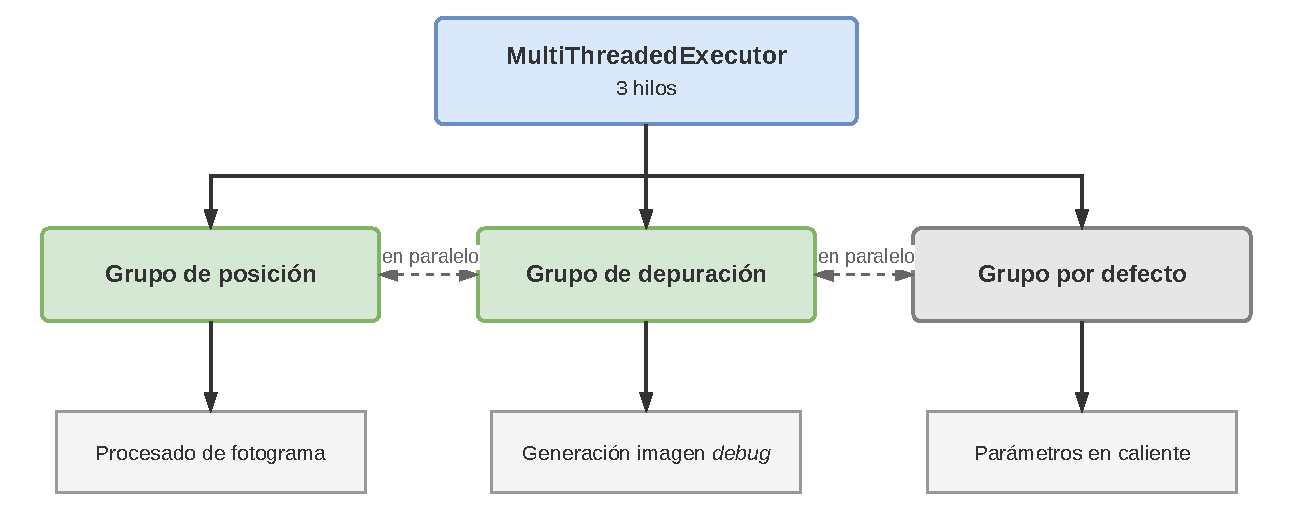
\includegraphics[width=\textwidth]{imaxes/IMPLEMENTACION/multithread_nodo_camara.pdf}
        \caption{Nodo de captura}
        \label{fig:executor-multihilo}
    \end{subfigure}

    \vspace{0.6em}
    \begin{subfigure}[b]{0.9\textwidth}
        \centering
        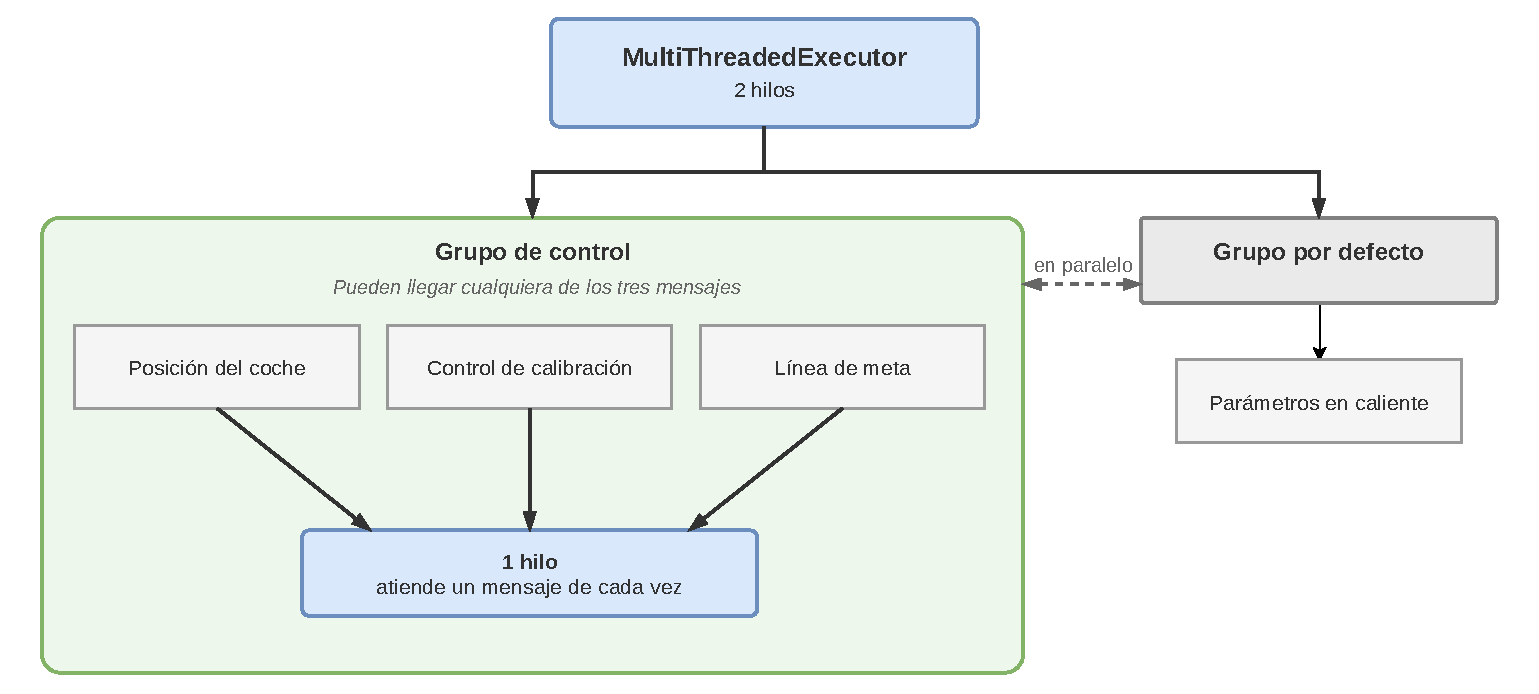
\includegraphics[width=\textwidth]{imaxes/IMPLEMENTACION/multithread_nodo_controlador.pdf}
        \caption{Nodo de control de carril}
        \label{fig:concurrencia-controlador}
    \end{subfigure}

    \vspace{0.6em}
    \begin{subfigure}[b]{0.8\textwidth}
        \centering
        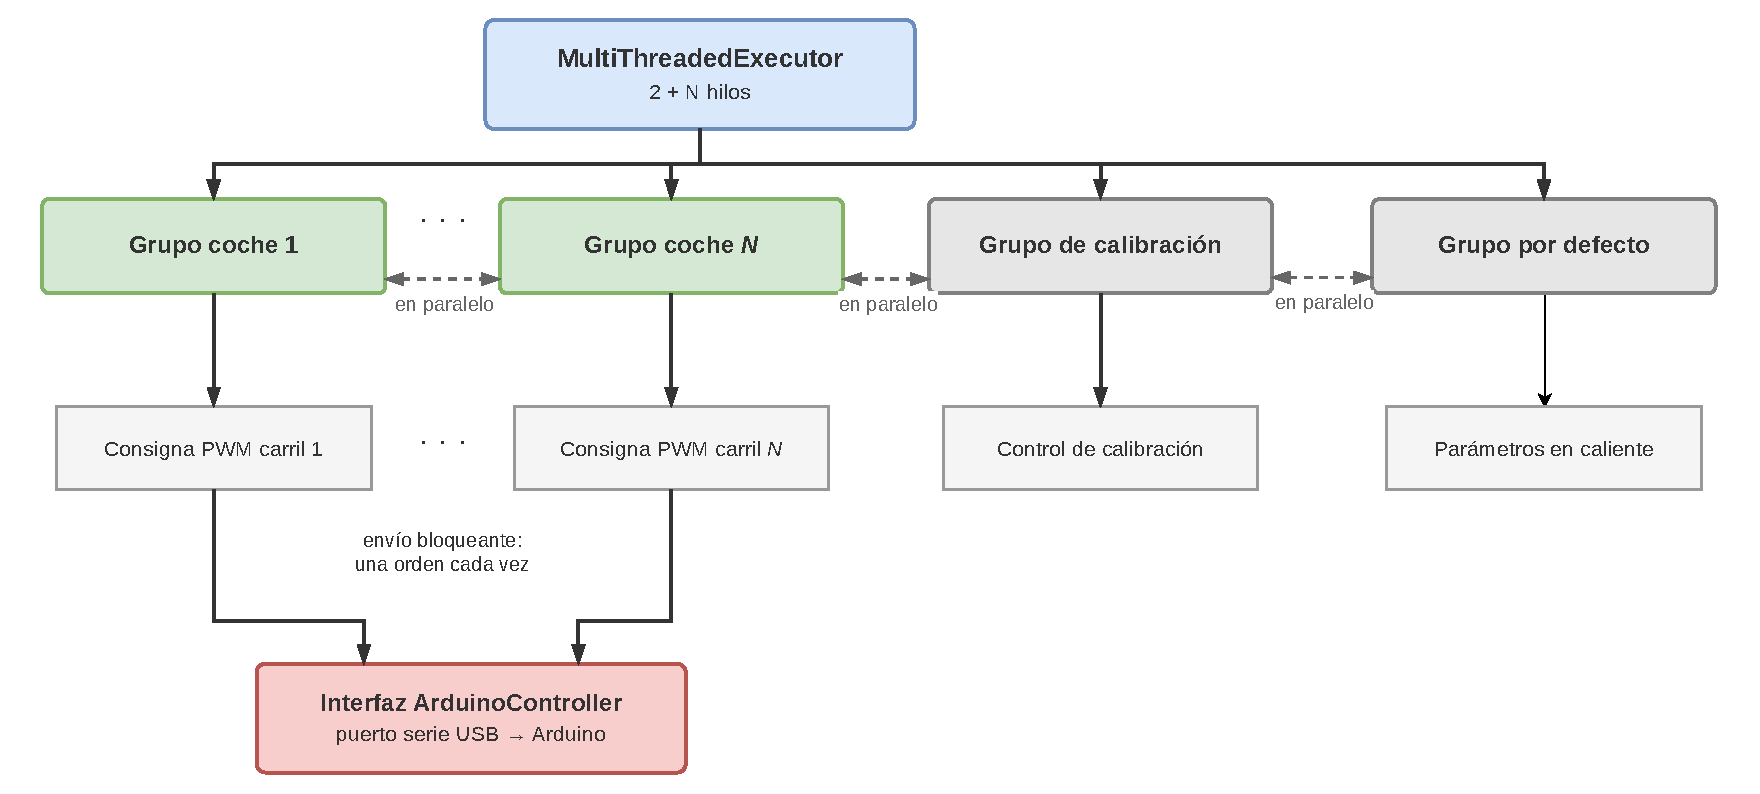
\includegraphics[width=\textwidth]{imaxes/IMPLEMENTACION/multithread_nodo_puente.pdf}
        \caption{Nodo puente}
        \label{fig:concurrencia-puente}
    \end{subfigure}
    \caption{Reparto de los \emph{callbacks} en grupos dentro de cada tipo de nodo. En los tres casos se conserva el grupo por defecto de ROS~2, atendido por un hilo propio, que es el que mantiene disponible la reconfiguración en caliente.}
    \label{fig:concurrencia-nodos}
\end{figure}

El nodo de captura es el más exigente, porque atiende dos tareas de coste muy distinto: obtener las posiciones de los coches y generar las imágenes de depuración. Cada una tiene su grupo, de modo que la segunda nunca retrasa a la primera. Dentro del procesamiento hay además un segundo nivel de concurrencia, porque buscar varios coches en un mismo fotograma multiplica el trabajo por vehículo. Se resolvió con un patrón productor-consumidor (figura~\ref{fig:modelo-hilos-camara}): el productor recoge los fotogramas que entrega la cámara cada \qty{33}{\milli\second} y un \emph{timer} de ROS~2 toma el último y lanza su procesamiento sobre un \emph{ThreadPool} con un trabajador por coche. Como la búsqueda de cada coche es independiente de las demás, todas se ejecutan sobre el mismo fotograma a la vez y el consumidor espera a que terminen antes de darlo por procesado. Un \emph{flag} impide que un disparo se solape con un procesamiento en curso: si el análisis se prolonga, los disparos intermedios se descartan en lugar de encolarse, con lo que el nodo degrada su cadencia pero nunca acumula retraso.

\begin{figure}[tbp]
    \centering
    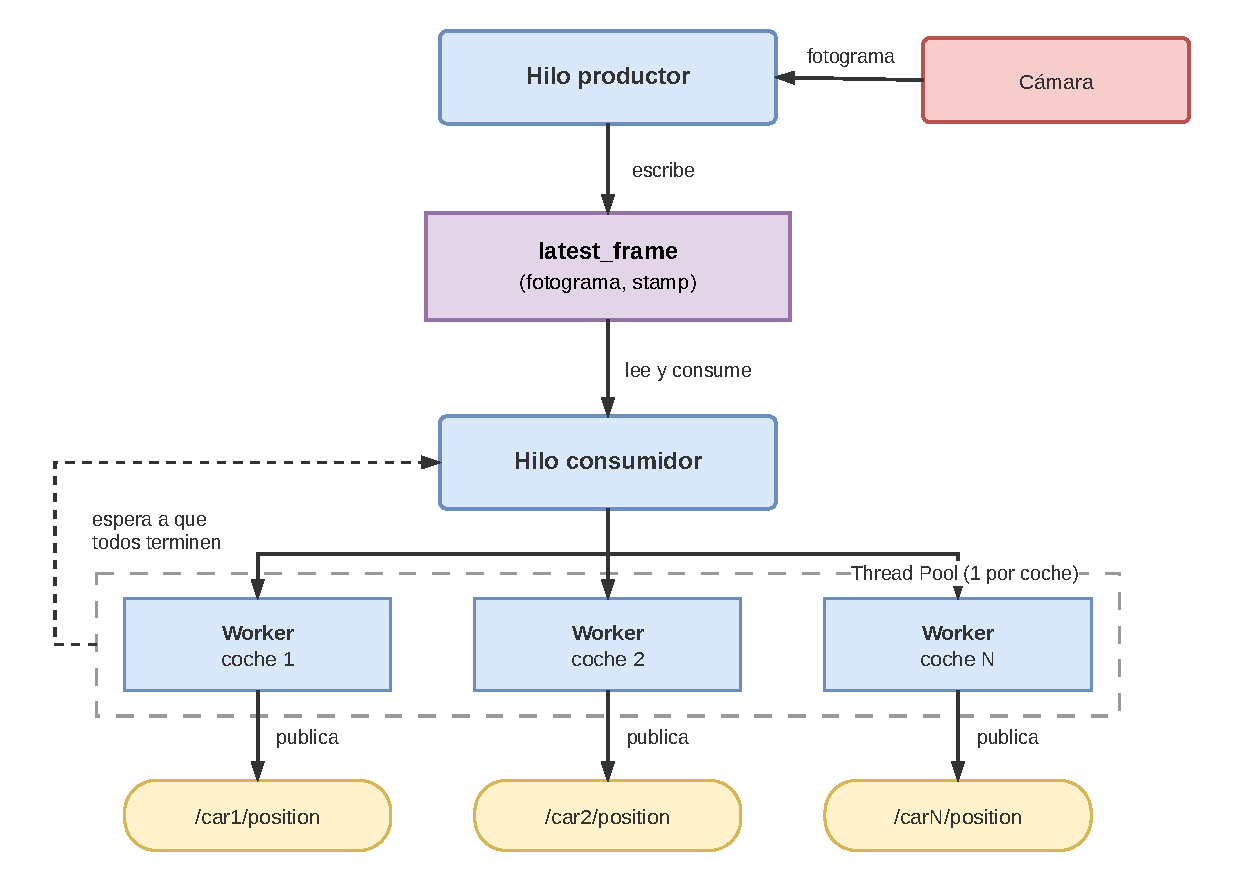
\includegraphics[width=0.75\textwidth]{imaxes/IMPLEMENTACION/productor_consumidor_nodo_camara.pdf}
    \caption{Modelo productor-consumidor con el que el nodo de cámara busca todos los coches sobre un mismo fotograma.}
    \label{fig:modelo-hilos-camara}
\end{figure}

Los otros dos nodos solo necesitan concurrencia a nivel de nodo. El controlador recibe la posición del coche, la orden de cambio de modo y la línea de meta, y como los tres modifican el mismo estado van a un único grupo, con lo que el estado del algoritmo queda siempre en manos de un solo hilo. El puente, en cambio, crea un grupo por controlador desplegado, ya que cada uno publica en su propio \emph{topic} y así el retraso de un carril no impide atender los demás. Esa concurrencia, sin embargo, no llega al envío: hay un único Arduino y un único puerto serie, y la propia interfaz de comunicación serializa el acceso (sección~\ref{subsec:actuacion-interfaz}).

\section{Detección de las pegatinas}
\label{sec:nodo-camara}
\label{subsec:deteccion-etiquetas}

Todo lo que el sistema sabe de un coche sale de localizar sus dos pegatinas en la imagen, y ese procedimiento se hereda del trabajo de Mario López~\cite{tfgmario}. El fotograma se convierte al espacio HSV, que resiste mejor las variaciones de iluminación, y se genera una máscara binaria por pegatina con los píxeles que caen dentro del rango de su color, predefinido para cada uno de los siete colores admitidos. Sobre esa máscara se encadenan una apertura morfológica, que elimina los píxeles aislados, y un cierre, que rellena los huecos de las regiones válidas. De los contornos externos resultantes se toma el mayor, se descarta si no supera un área mínima configurable y se obtienen su rectángulo delimitador y su centroide. La figura~\ref{fig:deteccion-color} recorre estas etapas sobre un fotograma real.

\begin{figure}[tbp]
    \centering
    \begin{subfigure}[b]{0.48\textwidth}
        \centering
        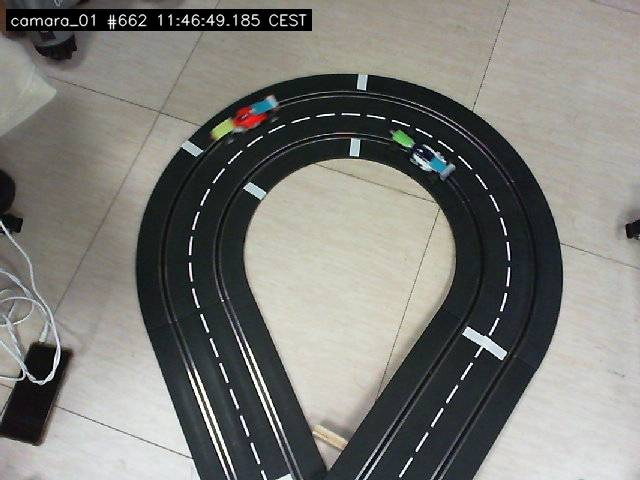
\includegraphics[width=\textwidth]{imaxes/IMPLEMENTACION/det_color_a_original.png}
        \caption{Fotograma capturado}
        \label{fig:deteccion-color-a}
    \end{subfigure}
    \hfill
    \begin{subfigure}[b]{0.48\textwidth}
        \centering
        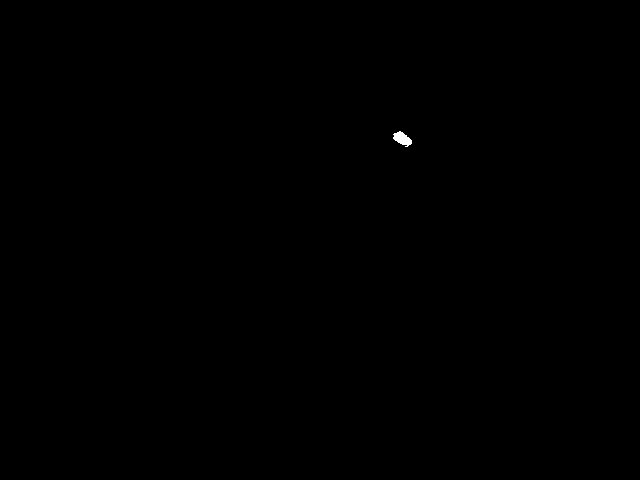
\includegraphics[width=\textwidth]{imaxes/IMPLEMENTACION/det_color_b_mascara.png}
        \caption{Máscara del color de la pegatina delantera}
        \label{fig:deteccion-color-b}
    \end{subfigure}

    \vspace{0.7em}
    \begin{subfigure}[b]{0.34\textwidth}
        \centering
        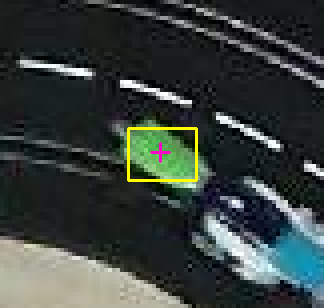
\includegraphics[width=\textwidth]{imaxes/IMPLEMENTACION/det_color_c_resultado.png}
        \caption{Rectángulo y centroide}
        \label{fig:deteccion-color-c}
    \end{subfigure}
    \caption{Etapas de la detección por color de una de las pegatinas del coche.}
    \label{fig:deteccion-color}
\end{figure}

Lo que cambia entre los dos modos de funcionamiento (sección~\ref{sec:modos_funcionamiento}) no es este procedimiento, sino la región del fotograma sobre la que se aplica: la imagen completa durante la calibración y una región reducida durante la carrera.

\section{La vuelta de calibración}
\label{subsec:modos-funcionamiento}
\label{subsec:control-modos}

La calibración produce dos cosas a la vez, una en la cámara y otra en el controlador, a partir del mismo flujo de detecciones de la pegatina delantera. Basta con la delantera porque es la que da una trayectoria limpia~\cite{tfgadrian}: la trasera puede quedar oculta a ratos y la ruta base debe registrarse sin interrupciones. Como consecuencia, las pegatinas delanteras sí deben ser de distinto color entre coches, mientras que dos coches pueden compartir la trasera.

En la cámara, cada detección se acumula hasta que el coche cierra su vuelta; con esos puntos se genera una máscara que restringe la búsqueda de ese coche a una franja alrededor del recorrido conocido (figura~\ref{fig:mascara-trayectoria}). Esa franja deja fuera el carril contrario, con lo que el coche que circula por él deja de ser un falso positivo posible. La calibración termina coche a coche y no para todo el sistema: la cámara se suscribe al \emph{topic} de calibración de cada vehículo configurado y genera su máscara al recibir el aviso correspondiente, de modo que un coche puede estar ya en carrera mientras otro sigue dando su vuelta de reconocimiento.

\begin{figure}[tbp]
    \centering
    \begin{subfigure}[b]{0.32\textwidth}
        \centering
        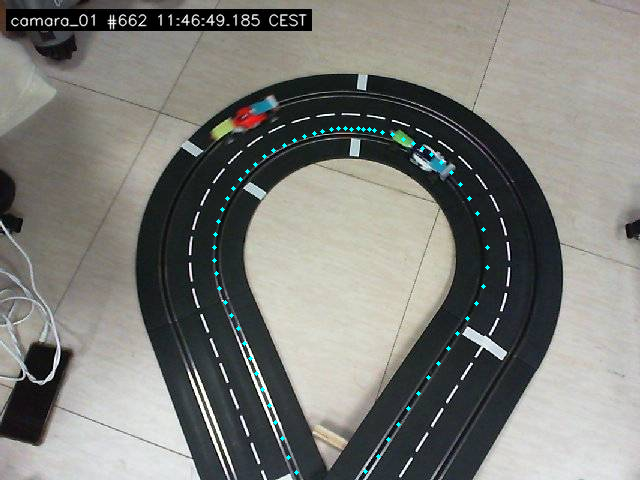
\includegraphics[width=\textwidth]{imaxes/IMPLEMENTACION/mascara_a_puntos.png}
        \caption{Posiciones acumuladas}
        \label{fig:mascara-trayectoria-a}
    \end{subfigure}
    \hfill
    \begin{subfigure}[b]{0.32\textwidth}
        \centering
        
\includegraphics[width=\textwidth]{imaxes/IMPLEMENTACION/mascara_b_mascara.png}
        \caption{Máscara generada}
        \label{fig:mascara-trayectoria-b}
    \end{subfigure}
    \hfill
    \begin{subfigure}[b]{0.32\textwidth}
        \centering
        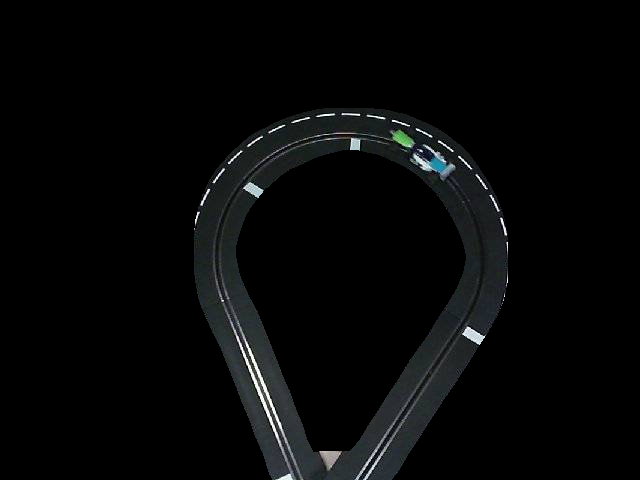
\includegraphics[width=\textwidth]{imaxes/IMPLEMENTACION/mascara_c_filtrado.png}
        \caption{Fotograma filtrado}
        \label{fig:mascara-trayectoria-c}
    \end{subfigure}
    \caption{Generación de la máscara de trayectoria de un coche a partir de su vuelta de calibración.}
    \label{fig:mascara-trayectoria}
\end{figure}

En el controlador, las mismas posiciones se acumulan en un diccionario indexado por cámara: cada nodo de captura del que recibe mensajes tiene su propia lista de puntos y en ningún momento se construye una lista única con el circuito completo. Lo que delimita la acumulación es el paso por meta. Los puntos se recogen entre el primer cruce y el segundo, de modo que cada trayectoria base es exactamente una vuelta que empieza en la meta y todo lo anterior —colocar el coche, arrancarlo y las vueltas que dé mientras se levanta el sistema— se descarta. Al cerrarse la vuelta el controlador lo notifica en su \emph{topic} de calibración, filtra cada lista descartando los puntos que queden a menos de un umbral del último aceptado y crea una instancia del algoritmo por cámara, a la que inyecta su trayectoria. Lo aprendido se vuelca en disco en ficheros JSON, que los nodos cargan al arrancar para saltarse la calibración cuando ni las cámaras ni el circuito se han movido.
\label{subsec:cache-calibracion}

Que la calibración se cierre sola es un requisito de la arquitectura, no una comodidad. En los trabajos previos la arrancaba y la daba por concluida una persona desde una interfaz gráfica: había que delimitar el coche con un rectángulo y marcar la meta a mano~\cite{tfgmario}, o seleccionar el vehículo, activar la búsqueda y confirmar los valores obtenidos~\cite{tfgadrian}. Con los nodos repartidos entre varias máquinas y sin una interfaz desde la que supervisarlos, la única forma de delimitar la vuelta es con la información que ya circula por la red, y esa información es el paso por meta que el propio controlador detecta.

\section{Seguimiento en carrera}
\label{subsec:seguimiento-roi}

Cerrada la calibración, la búsqueda deja de recorrer el fotograma entero y se restringe a una región de interés de $150 \times 150$ píxeles centrada en la posición predicha para el coche, obtenida por la extrapolación lineal que introdujo Mario López~\cite{tfgmario}: conocidas las dos últimas posiciones, el centro de la región es la actual más el vector de movimiento del último fotograma. Sobre ella se aplica además la máscara de trayectoria, de modo que solo sobreviven los píxeles que pertenecen a la vez a la región y a las proximidades del carril; la intersección de ambos filtros procede también de los trabajos previos~\cite{tfgmario,tfgadrian}. La figura~\ref{fig:roi-filtrado} muestra el proceso completo, y su último panel es lo único que llega al detector de color. El precio de trabajar sobre un recorte es que las coordenadas obtenidas son relativas a la región y hay que trasladarlas al sistema de referencia de la cámara antes de publicarlas.

\begin{figure}[tbp]
    \centering
    \begin{subfigure}[b]{0.55\textwidth}
        \centering
        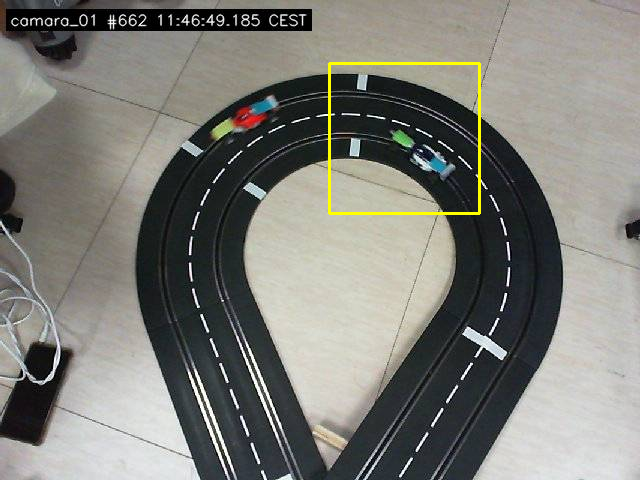
\includegraphics[width=\textwidth]{imaxes/IMPLEMENTACION/roi_a_recuadro.png}
        \caption{Región marcada sobre el fotograma}
        \label{fig:roi-filtrado-a}
    \end{subfigure}
    \hfill
    \begin{subfigure}[b]{0.38\textwidth}
        \centering
        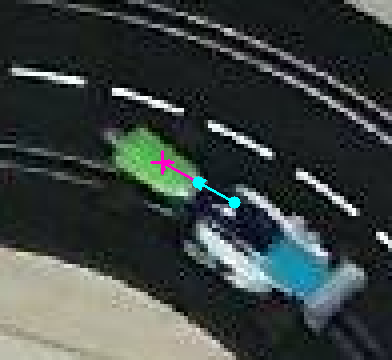
\includegraphics[width=\textwidth]{imaxes/IMPLEMENTACION/roi_b_extrapolacion.png}
        \caption{Extrapolación de la posición}
        \label{fig:roi-filtrado-b}
    \end{subfigure}

    \vspace{0.7em}
    \begin{subfigure}[b]{0.32\textwidth}
        \centering
        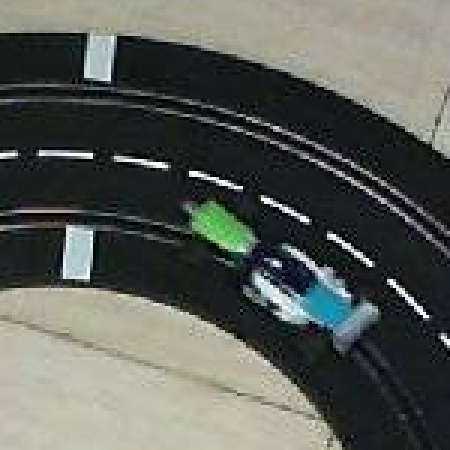
\includegraphics[width=\textwidth]{imaxes/IMPLEMENTACION/roi_c_recorte.png}
        \caption{Recorte de la región}
        \label{fig:roi-filtrado-c}
    \end{subfigure}
    \hspace{0.04\textwidth}
    \begin{subfigure}[b]{0.32\textwidth}
        \centering
        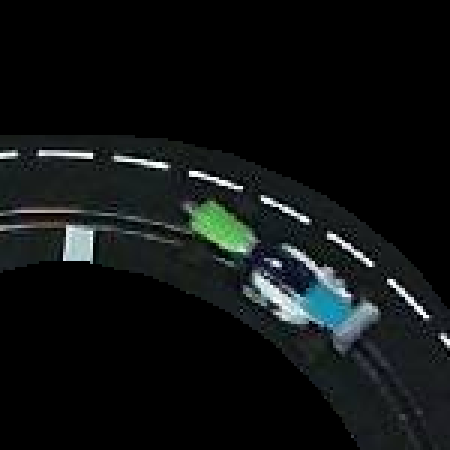
\includegraphics[width=\textwidth]{imaxes/IMPLEMENTACION/roi_d_filtrado.png}
        \caption{Intersección con la máscara}
        \label{fig:roi-filtrado-d}
    \end{subfigure}
    \caption{Acotación de la búsqueda en modo carrera. En el detalle, las dos flechas encadenadas son el desplazamiento medido entre los dos últimos fotogramas y la cruz marca la posición predicha, que en este caso cae a 1,6~píxeles de la real.}
    \label{fig:roi-filtrado}
\end{figure}

Las oclusiones son habituales en un circuito de Scalextric~\cite{tfgmario} y un derrape brusco puede alejar el coche de la posición predicha, así que hay que contar con perder el seguimiento y recuperarlo.
\label{subsec:readquisicion}
La estrategia es ampliar progresivamente la zona de búsqueda: cada fotograma sin detección incrementa el tamaño de la región en 50~píxeles, hasta abarcar como máximo la imagen completa. Los trabajos previos pasaban de golpe a examinar toda la proximidad de la trayectoria; el crecimiento gradual acota el coste de los fotogramas inmediatamente posteriores a la pérdida, que son los más probables. Al perder el seguimiento se descartan además las posiciones anteriores, como ya hacía Mario López~\cite{tfgmario}, para que la extrapolación no combine un punto previo a la pérdida con el primero posterior y sitúe la región lejos del coche; la primera detección tras readquirir vuelve a centrarla sobre la posición encontrada.

Por último, el nodo ofrece un modo de depuración, desactivado por defecto y activable en caliente, que conserva una copia del fotograma procesado y dibuja sobre él los rectángulos de las pegatinas, una cruceta en cada centroide y, en una esquina, el identificador del nodo, el número de fotograma y la hora de captura. Esa imagen se publica como \emph{vista de la cámara} y es la que permite seguir cada cámara en directo y la que graba el sistema de visualización (sección~\ref{sec:sistema-visualizacion}).
\label{subsec:modo-depuracion}

\section{La meta y los tiempos por vuelta}
\label{subsec:deteccion-meta}
\label{sec:control-rail}

La línea de meta se señaliza con una etiqueta alargada de un color reservado que atraviesa la pista y se detecta una sola vez, al arrancar el nodo, porque su posición no cambia durante la carrera. El procedimiento es el de Adrián Rego~\cite{tfgadrian} y arranca igual que la detección de las pegatinas, con la máscara del color en HSV, pero el cierre morfológico se aplica con un \emph{kernel} mucho mayor: los raíles y las ranuras de la pista atraviesan la etiqueta y la fragmentan en trozos que hay que volver a unir en una única región (figura~\ref{fig:deteccion-meta}). Sobre ella se calcula el rectángulo de área mínima que la encierra, que a diferencia del delimitador convencional puede estar rotado y se adapta así a la orientación real de la línea; de sus cuatro vértices se identifican los dos lados cortos comparando las aristas adyacentes, y el segmento que une sus puntos medios define la meta. Cada cámara la busca al arrancar y, si no la ve, no publica nada, de modo que en un despliegue multicámara solo la publica la que la observa y no hay que designar de antemano una cámara de meta.

\begin{figure}[tbp]
    \centering
    \begin{subfigure}[b]{0.32\textwidth}
        \centering
        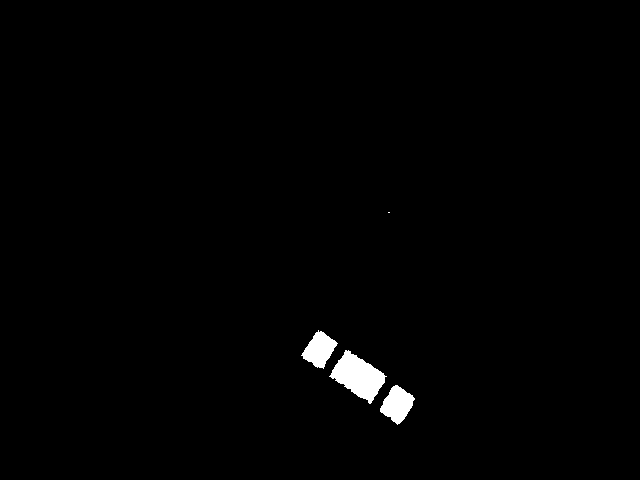
\includegraphics[width=\textwidth]{imaxes/IMPLEMENTACION/meta_a_mascara.png}
        \caption{Máscara del color de la meta}
        \label{fig:deteccion-meta-a}
    \end{subfigure}
    \hfill
    \begin{subfigure}[b]{0.32\textwidth}
        \centering
        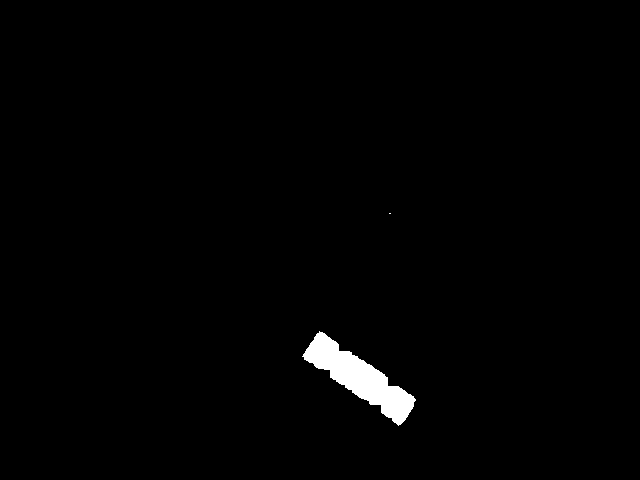
\includegraphics[width=\textwidth]{imaxes/IMPLEMENTACION/meta_b_cierre.png}
        \caption{Tras el cierre morfológico}
        \label{fig:deteccion-meta-b}
    \end{subfigure}
    \hfill
    \begin{subfigure}[b]{0.32\textwidth}
        \centering
        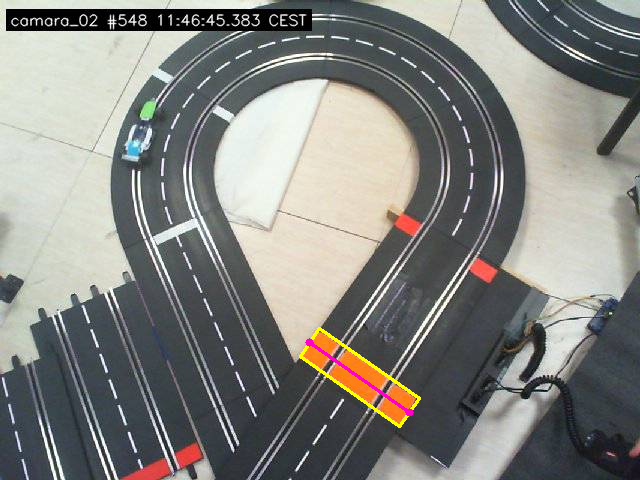
\includegraphics[width=\textwidth]{imaxes/IMPLEMENTACION/meta_c_segmento.png}
        \caption{Rectángulo y segmento}
        \label{fig:deteccion-meta-c}
    \end{subfigure}
    \caption{Detección de la línea de meta en la cámara~2. Los raíles parten la etiqueta en tres trozos que el cierre vuelve a unir.}
    \label{fig:deteccion-meta}
\end{figure}

Con ese segmento, el controlador cuenta las vueltas de su coche y mide su duración, que es lo que cierra el ciclo de aprendizaje del algoritmo (sección~\ref{subsec:algoritmo-aprendizaje}).
\label{subsec:control-meta}
El mecanismo se hereda de Mario López~\cite{tfgmario} y solo se aplica a los mensajes de la cámara que publicó la meta: para cada posición se calcula el producto vectorial entre el vector que recorre el segmento y el que va de uno de sus extremos a la pegatina delantera, y su signo indica de qué lado de la recta está el coche, de modo que un cambio de signo entre dos fotogramas consecutivos significa que lo ha cruzado (figura~\ref{fig:producto-vectorial}). El instante exacto se aproxima interpolando entre los dos fotogramas implicados, con la fracción del intervalo que se obtiene del cociente entre la distancia del anterior y la suma de ambas; sin interpolar, tomar la marca del fotograma que detecta el cruce introduciría un error de hasta un período de captura en cada vuelta. Los instantes interpolados son las marcas de tiempo que la cámara pone al capturar, no el momento en que llega el mensaje (sección~\ref{subsec:qos}), con lo que no hace falta sincronizar los relojes de las máquinas: el tiempo por vuelta se calcula siempre contra la misma referencia.

\begin{figure}[tbp]
    \centering
    \begin{subfigure}[b]{0.48\textwidth}
        \centering
        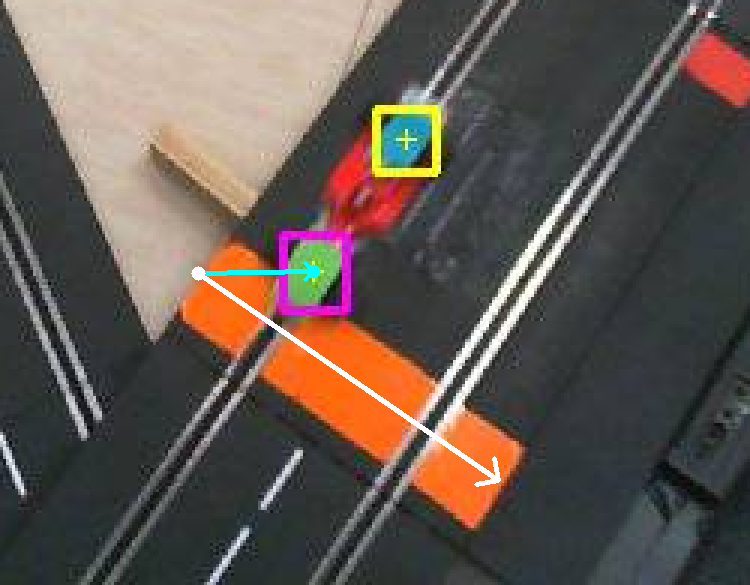
\includegraphics[width=\textwidth]{imaxes/IMPLEMENTACION/meta_vector_a_antes.png}
        \caption{Antes de cruzar}
        \label{fig:producto-vectorial-a}
    \end{subfigure}
    \hfill
    \begin{subfigure}[b]{0.48\textwidth}
        \centering
        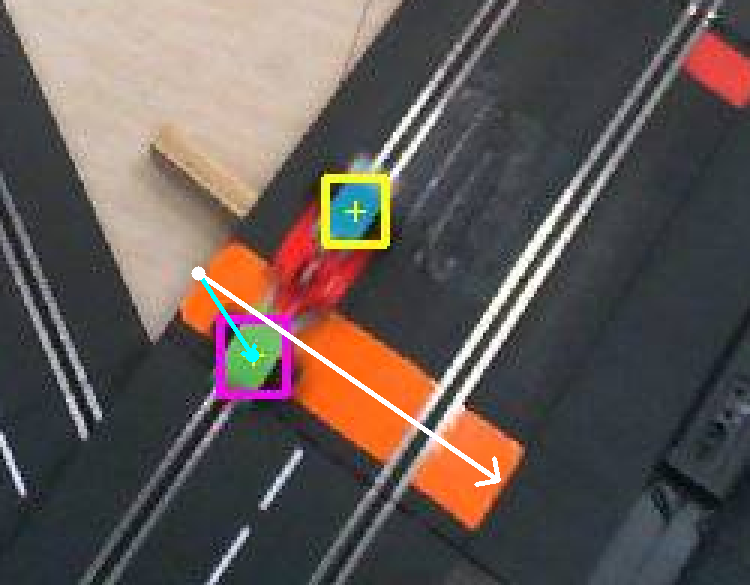
\includegraphics[width=\textwidth]{imaxes/IMPLEMENTACION/meta_vector_b_despues.png}
        \caption{Después de cruzar}
        \label{fig:producto-vectorial-b}
    \end{subfigure}
    \caption{Cambio de signo del producto vectorial al cruzar la línea de meta.}
    \label{fig:producto-vectorial}
\end{figure}

El método arrastra una limitación que ya señalaba Mario López~\cite{tfgmario}: el signo se calcula contra la recta infinita que contiene al segmento y, como el circuito es cerrado, esa recta vuelve a cortar la pista en otro punto, donde el signo cambia igual. Él lo evitaba exigiendo que el coche estuviese a menos de vez y media su longitud de un extremo de la meta; aquí el cambio de signo se ignora mientras la distancia de la pegatina al segmento supere un umbral configurable. Esta solución sustituye además a la de Adrián Rego~\cite{tfgadrian}, que fue la primera que se implementó y que fallaba la cuenta con el coche muy lento o detenido sobre la línea, mientras que el cambio de signo no depende de la velocidad a la que se cruce.

En cada cruce el controlador publica el tiempo y el número de vuelta en su \emph{topic} de telemetría y notifica el evento a todas las instancias del algoritmo, indicando si la vuelta fue limpia. Esto ocurre igual cuando el coche lo conduce una persona: en modo manual el controlador calibra, recibe posiciones, cuenta vueltas y publica telemetría exactamente igual, y lo único que no hace es publicar consigna, de forma que el puente nunca toca ese carril. Sirve para registrar una carrera conducida por una persona con el mismo formato de datos que una automática y poder compararlas después con la herramienta de análisis (sección~\ref{subsec:visualizacion-analisis}).
\label{subsec:control-automatico-manual}

\section{Implementación del algoritmo de velocidad}
\label{sec:implementacion-algoritmo}

El algoritmo diseñado en la sección~\ref{sec:algoritmo-arquitectura} recibe una posición del coche sobre la imagen de una cámara y devuelve el valor de PWM que hay que aplicar al carril, o bien la indicación de descartar el fotograma, en cuyo caso el controlador mantiene el último valor válido. Todo lo que decide sale de la trayectoria aprendida durante la calibración y de la desviación que el coche muestra respecto a ella.

\subsection{Instancias por cámara}
\label{subsec:algoritmo-instancias}

El algoritmo no trabaja sobre el circuito completo, sino sobre la porción que observa una cámara: cada lista de puntos del diccionario del controlador da lugar a una instancia independiente, con su propia cadena de celdas, sus propias zonas y su propio perfil de PWM. No existe, por tanto, una trayectoria global ni un sistema de referencia común, y ninguna instancia sabe nada de las demás; el único punto del proyecto donde todas se llevan a un plano común es la herramienta de análisis en diferido (sección~\ref{subsec:visualizacion-analisis}), que queda fuera del lazo de control. La alternativa, fusionar las trayectorias en un mapa único, exigiría calibrar la posición relativa de las cámaras y aportaría poco a un control que solo necesita saber dónde está el coche dentro del tramo que se está viendo.

La visión de conjunto la aporta el controlador, que enruta cada posición a la instancia de la cámara que la originó según el campo \texttt{camara\_id} del mensaje (sección~\ref{subsec:mensajes-propios}), decide qué cámara está activa, cierra un derrape en una y abre su continuación en la siguiente, propaga hacia atrás las reducciones que no caben en una porción y determina si una vuelta ha sido limpia en todo el trazado. Esos mecanismos se describen en la sección~\ref{subsec:algoritmo-coordinacion}.

\subsection{Cadena de celdas y localización del coche}
\label{subsec:algoritmo-celdas}
\label{subsec:algoritmo-localizacion}

La trayectoria base (sección~\ref{subsec:trayectoria-base}) se transforma en una sucesión ordenada de celdas equiespaciadas. El remuestreo es necesario porque los puntos crudos no están repartidos de forma uniforme: su separación depende de la velocidad que llevase el coche al grabarlos y de si todas las posiciones enviadas por la cámara llegaron al controlador. Se recorre la trayectoria colocando una celda cada cierta distancia fija e interpolando entre puntos consecutivos, de modo que las celdas quedan repartidas sobre el recorrido real con independencia de cómo cayeran los puntos originales. Los saltos que superan un umbral reciben otro tratamiento, porque corresponden a tramos que la cámara no ve —un puente, un túnel— y dentro de ellos no hay nada que interpolar: se crea una única \emph{celda gigante} que registra la longitud real del hueco y que se trata entera con un mismo valor de PWM, sin poder localizar el coche ni detectar derrapes en su interior.

Sobre esa cadena se sitúan las dos pegatinas. Para cada una se busca la celda más próxima al centroide y después se proyecta el centroide sobre los dos segmentos que unen esa celda con la anterior y la posterior, conservando la menor de las dos distancias; la proyección hace falta porque medir contra el punto de la celda daría una distancia dependiente de dónde caiga la celda, mientras que contra los segmentos se obtiene la distancia perpendicular a la trayectoria. Por eso tampoco puede proyectarse a través de una celda gigante, donde no hay trayectoria conocida sobre la que hacerlo. Cada distancia tiene después un uso distinto: la de la delantera es una comprobación de que el coche sigue el recorrido esperado, y si supera un umbral la detección se considera inválida y el fotograma se descarta sin calcular PWM; la de la trasera es la señal con la que se detectan los derrapes.

\subsection{Detección de derrapes}
\label{subsec:algoritmo-derrapes}

La arquitectura exige una señal capaz de indicar en qué punto del circuito el coche ha perdido el control (sección~\ref{subsec:derrape-arquitectura}), y la escogida es esa distancia perpendicular de la pegatina trasera: cuando la parte trasera del coche se abre, la distancia crece mientras la delantera sigue marcando la posición sobre el trazado. La detección es una máquina de estados que se alimenta en cada fotograma con la celda y la distancia de la trasera: al superarse el umbral se abre un derrape y se anota su celda inicial, mientras se mantenga por encima se prolonga actualizando la final, y al caer por debajo se cierra. No se abren derrapes junto a los extremos de la cadena ni junto a las celdas gigantes, donde la medida no es fiable.

La figura~\ref{fig:secuencia-derrape} recoge un caso real. Con el coche alineado la pegatina trasera va sobre el carril y su distancia es casi nula; al abrirse la parte trasera la distancia crece hasta superar el umbral, que es lo que abre el derrape, y en el instante más violento el coche queda atravesado y no se detecta ninguna de las dos pegatinas, situación que resuelve la readquisición de la sección~\ref{subsec:readquisicion}.

\begin{figure}[tbp]
    \centering
    \begin{subfigure}[b]{0.48\textwidth}
        \centering
        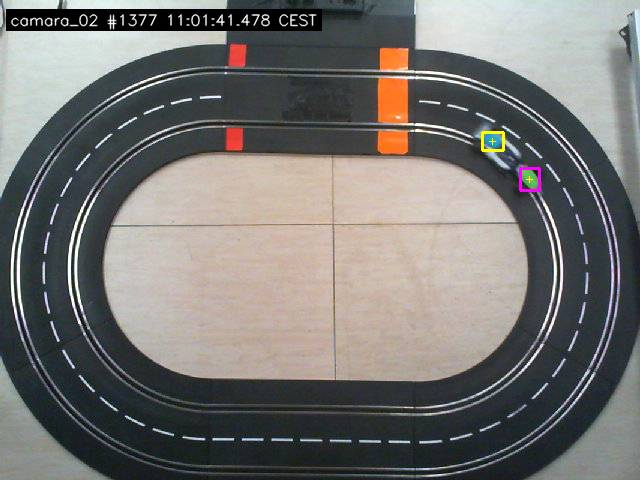
\includegraphics[width=\textwidth]{imaxes/IMPLEMENTACION/derrape_seq_a_antes.png}
        \caption{Coche alineado con el carril}
        \label{fig:secuencia-derrape-a}
    \end{subfigure}
    \hfill
    \begin{subfigure}[b]{0.48\textwidth}
        \centering
        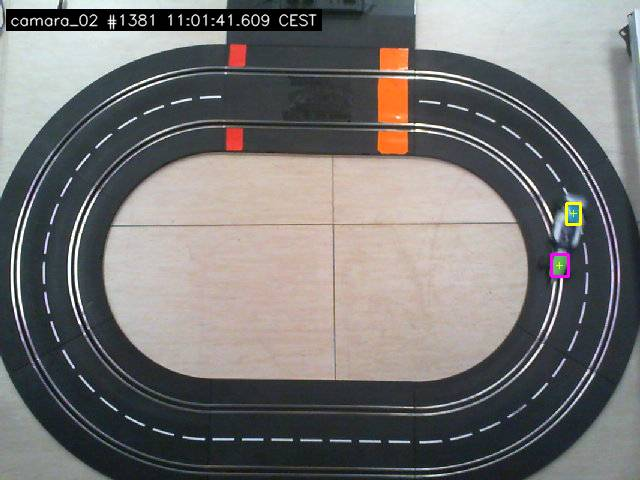
\includegraphics[width=\textwidth]{imaxes/IMPLEMENTACION/derrape_seq_b_inicio.png}
        \caption{La parte trasera empieza a abrirse}
        \label{fig:secuencia-derrape-b}
    \end{subfigure}

    \vspace{0.7em}
    \begin{subfigure}[b]{0.48\textwidth}
        \centering
        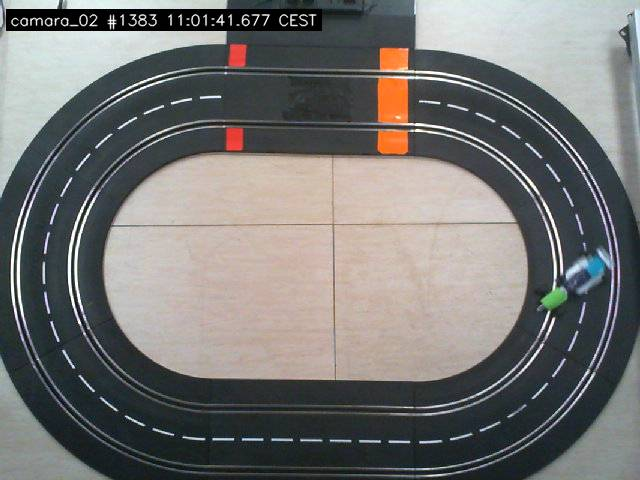
\includegraphics[width=\textwidth]{imaxes/IMPLEMENTACION/derrape_seq_c_completo.png}
        \caption{Derrape completo, sin detección}
        \label{fig:secuencia-derrape-c}
    \end{subfigure}
    \hfill
    \begin{subfigure}[b]{0.48\textwidth}
        \centering
        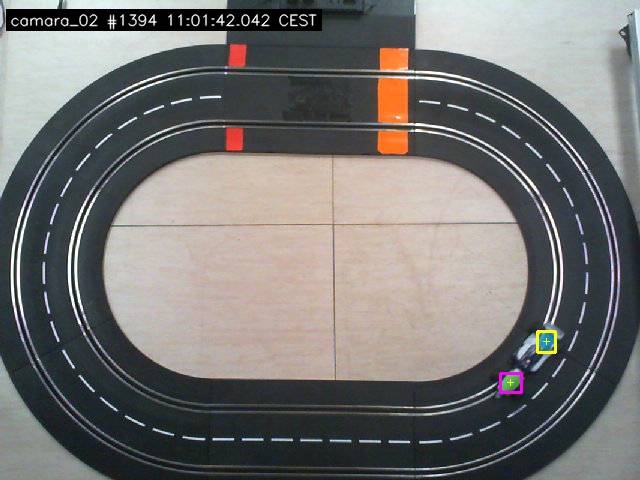
\includegraphics[width=\textwidth]{imaxes/IMPLEMENTACION/derrape_seq_d_recuperado.png}
        \caption{Seguimiento readquirido}
        \label{fig:secuencia-derrape-d}
    \end{subfigure}
    \caption{Secuencia de un derrape en el circuito con forma de óvalo.}
    \label{fig:secuencia-derrape}
\end{figure}

\subsection{Castigo de zonas y ciclo de aprendizaje}
\label{subsec:algoritmo-aprendizaje}

Cada instancia mantiene la partición de su cadena en zonas y aplica sobre ellas las dos políticas definidas en la sección~\ref{subsec:zonas-politicas}. El castigo se dispara al cerrarse un derrape: su intervalo de celdas se extiende hacia atrás una distancia fija en píxeles, que es el tramo de anticipación que exige la arquitectura, y el resultado se convierte en una zona de derrape cuyo PWM es el mínimo de los de las zonas que cubría el intervalo menos una reducción fija de dos unidades, con \texttt{minimum\_speed} como suelo. Si el derrape cae dentro o junto a una zona de derrape ya existente ambas se fusionan, y en ese caso el retroceso añadido es menor que el de una zona nueva, porque la existente ya aplicó el suyo al crearse; si cada reincidencia retrocediera la distancia completa, las zonas protegidas acabarían cubriendo el circuito entero y el perfil no volvería a subir en ningún tramo. Las celdas gigantes alcanzadas por un derrape o por su retroceso se castigan como una unidad, ya que dentro del hueco no hay precisión para distinguir una parte de otra.

La mejora se dispara con el paso por meta. El controlador comprueba si hubo algún derrape en alguna cámara durante la vuelta y comunica el resultado a todas las instancias; cada zona sin derrape sube su PWM en una unidad, con \texttt{maximum\_speed} como techo, salvo las que registraron uno en las últimas vueltas, que permanecen protegidas durante un número configurable de vueltas antes de poder volver a subir.

Las figuras~\ref{fig:derrape-trazas} y~\ref{fig:derrape-dist} recorren el ciclo completo sobre tres vueltas consecutivas de una sesión real. En la vuelta~21 la trasera va pegada a la trayectoria base, la distancia nunca se acerca al umbral y el PWM se mantiene constante en todo el recorrido, con una única zona. En la~22 la trasera se abre en la curva y la distancia supera el umbral durante diez fotogramas, lo que cierra un derrape y castiga la zona. En la~23 el perfil ya trae el PWM rebajado en ese tramo, visible como un escalón, y el coche vuelve a pasar limpio.

\begin{figure}[tbp]
    \centering
    \begin{subfigure}[b]{0.48\textwidth}
        \centering
        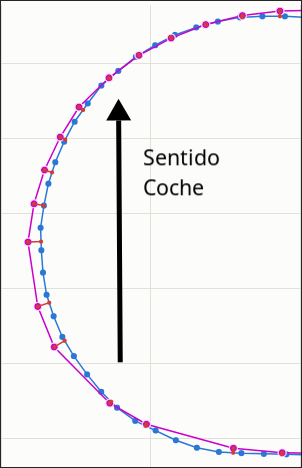
\includegraphics[width=\textwidth]{imaxes/IMPLEMENTACION/derrape_traza_v21.png}
        \caption{Vuelta 21, limpia}
        \label{fig:derrape-trazas-a}
    \end{subfigure}
    \hfill
    \begin{subfigure}[b]{0.48\textwidth}
        \centering
        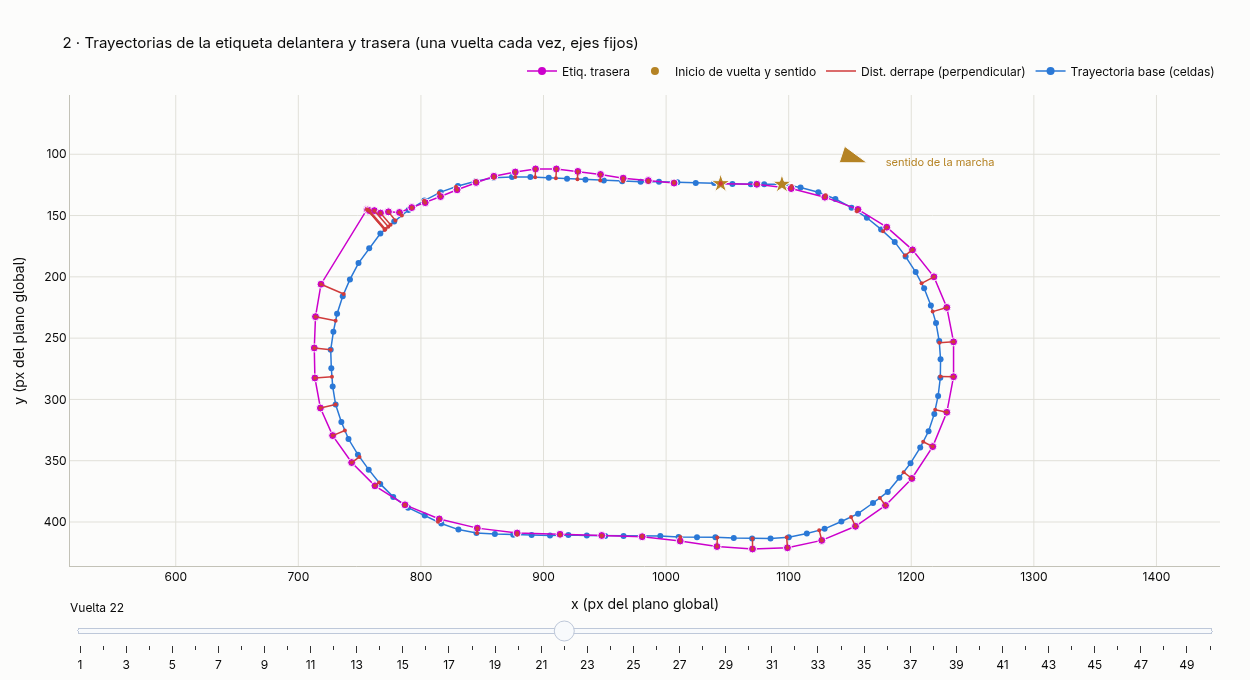
\includegraphics[width=\textwidth]{imaxes/IMPLEMENTACION/derrape_traza_v22.png}
        \caption{Vuelta 22, con derrape}
        \label{fig:derrape-trazas-b}
    \end{subfigure}

    \vspace{0.7em}
    \begin{subfigure}[b]{0.48\textwidth}
        \centering
        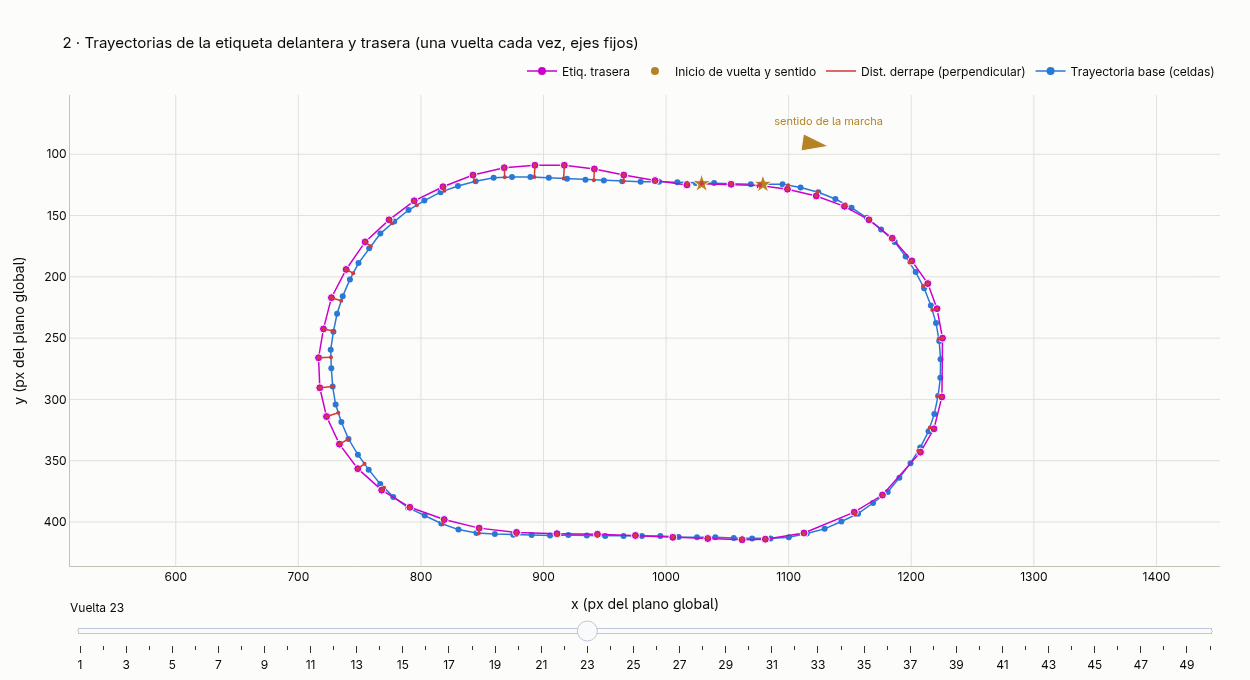
\includegraphics[width=\textwidth]{imaxes/IMPLEMENTACION/derrape_traza_v23.png}
        \caption{Vuelta 23, ya castigada}
        \label{fig:derrape-trazas-c}
    \end{subfigure}
    \caption{Recorrido de la pegatina trasera (magenta) frente a la trayectoria base (azul) en tres vueltas consecutivas. Los segmentos rojos son la distancia perpendicular que mide el algoritmo.}
    \label{fig:derrape-trazas}
\end{figure}

\begin{figure}[p]
    \centering
    \begin{subfigure}[b]{0.85\textwidth}
        \centering
        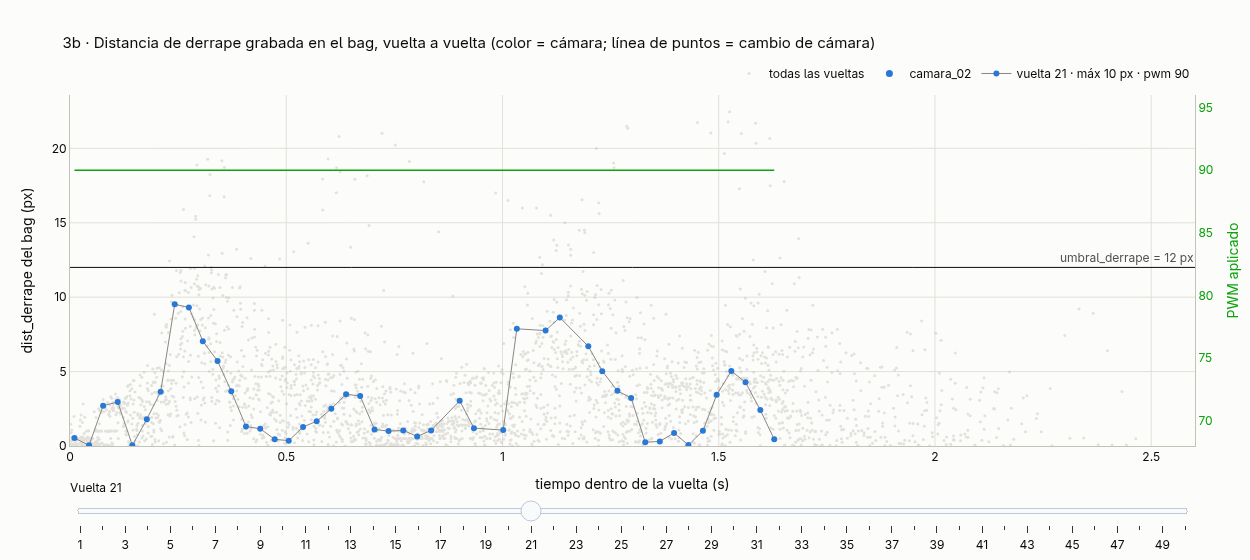
\includegraphics[width=\textwidth]{imaxes/IMPLEMENTACION/derrape_dist_v21.png}
        \caption{Vuelta 21}
        \label{fig:derrape-dist-a}
    \end{subfigure}

    \vspace{0.5em}
    \begin{subfigure}[b]{0.85\textwidth}
        \centering
        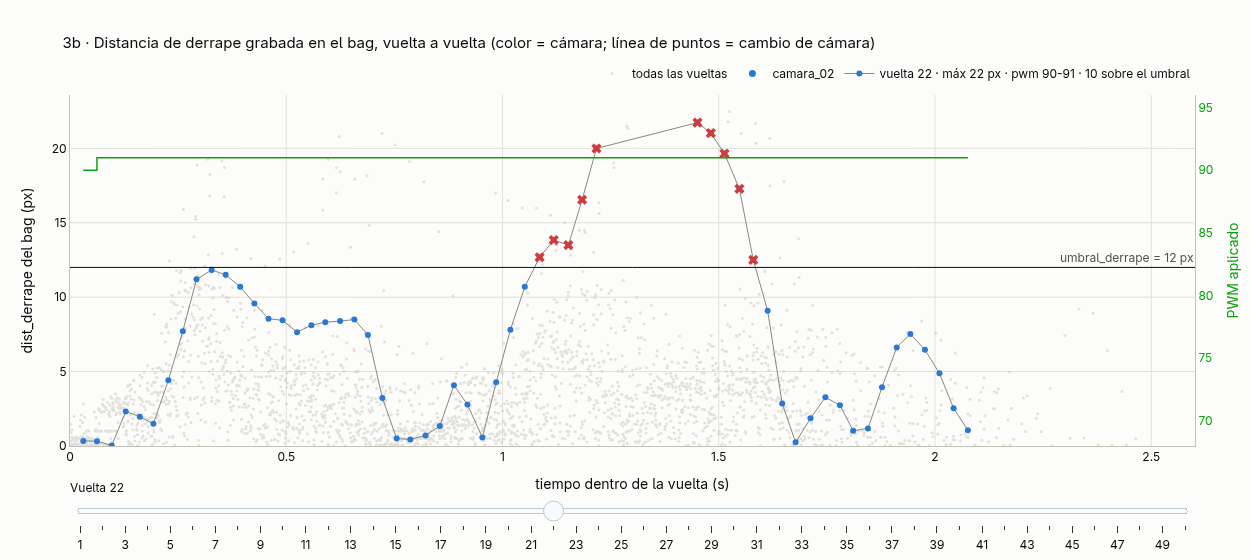
\includegraphics[width=\textwidth]{imaxes/IMPLEMENTACION/derrape_dist_v22.png}
        \caption{Vuelta 22}
        \label{fig:derrape-dist-b}
    \end{subfigure}

    \vspace{0.5em}
    \begin{subfigure}[b]{0.85\textwidth}
        \centering
        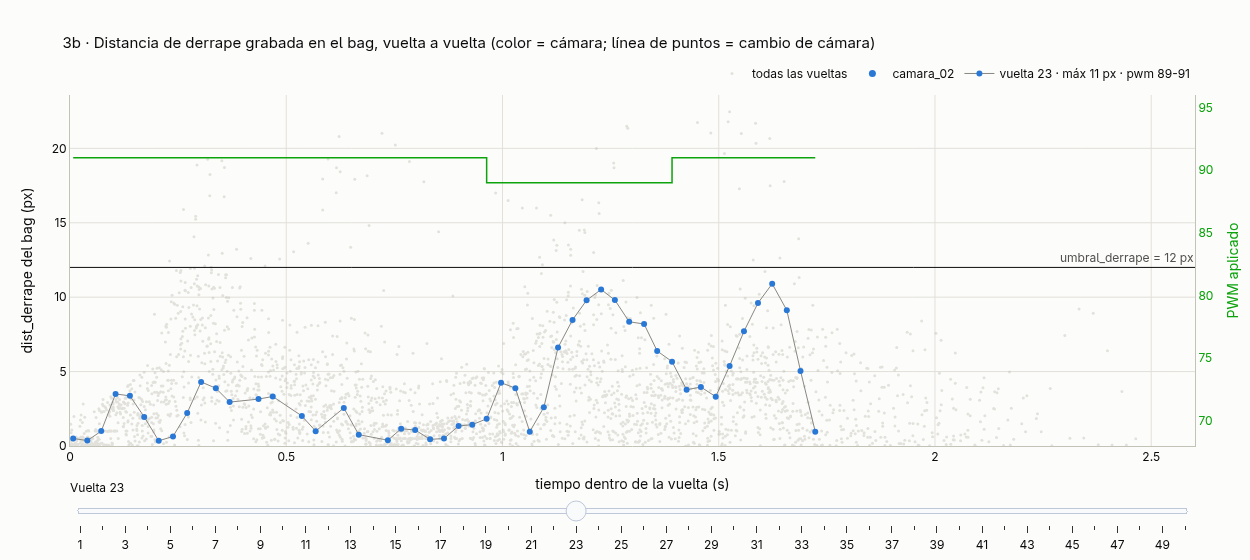
\includegraphics[width=\textwidth]{imaxes/IMPLEMENTACION/derrape_dist_v23.png}
        \caption{Vuelta 23}
        \label{fig:derrape-dist-c}
    \end{subfigure}
    \caption{Distancia de la pegatina trasera a lo largo de cada vuelta (eje izquierdo) frente al PWM aplicado (línea verde, eje derecho). Las aspas rojas marcan las muestras que superan el umbral y abren el derrape. El escalón verde de la vuelta~23 es la zona creada por el castigo de la anterior.}
    \label{fig:derrape-dist}
\end{figure}

\subsection{Coordinación entre cámaras}
\label{subsec:algoritmo-coordinacion}

Como cada instancia conoce solo su porción del circuito, hay tres situaciones que ninguna puede resolver sola y que asume el controlador.

La primera es la transición del coche entre cámaras. Cuando dos campos de visión se solapan ambas publican posiciones intercaladas del mismo coche, así que la cámara activa se mantiene mientras siga entregando fotogramas válidos y solo se cambia cuando deja de hacerlo durante un breve intervalo y otra sí está entregando. En cada cambio el controlador notifica la pérdida de visión a la cámara saliente y anota el relevo; como el coche recorre siempre el circuito en el mismo sentido, tras una vuelta completa ese registro contiene el orden secuencial de las cámaras, aprendido en carrera y sin ninguna configuración manual.

La segunda es el derrape repartido entre dos cámaras. Al recibir la notificación de pérdida de visión la instancia saliente cierra el derrape que tuviera abierto y, si seguía activo, la entrante recibe la orden de abrir uno nuevo, de modo que la zona se extiende entre cámaras y el derrape se detecta aunque el corte caiga en mitad de una curva.

La tercera es la propagación de reducciones, que ocurre cuando un derrape se produce cerca del inicio de la porción visible de una cámara, algo habitual si una curva queda repartida entre dos. El retroceso del castigo se sale por el inicio antes de agotarse y los píxeles restantes corresponden a un tramo de otra cámara, así que la instancia anota ese sobrante como reducción pendiente; el controlador lo recoge y, según el orden aprendido, ordena a la cámara precedente que lo aplique al final de su trayectoria, creando o ampliando allí la zona de derrape. Esa reducción externa no incrementa el contador de derrapes de quien la recibe, porque ya lo contabilizó la cámara que lo observó, pero la zona queda igualmente protegida. Si tampoco cupiera en la trayectoria de la cámara anterior, el sobrante volvería a quedar pendiente y seguiría propagándose hacia atrás hasta agotarse.

\section{Actuación sobre el circuito}
\label{sec:sistema-actuacion}
\label{subsec:actuacion-topics}

El nodo puente es puramente consumidor: no publica nada, se limita a suscribirse a los \emph{topics} en los que cada controlador anuncia el PWM de su carril, con una suscripción por coche declarado en la configuración. De cada mensaje extrae el carril y el valor, y le aplica dos comprobaciones antes de mandarlo al puerto serie. La primera es un filtro de repetición: el nodo guarda el último valor enviado a cada carril y descarta el mensaje si coincide. Como los controladores publican una consigna por cada posición recibida y el PWM se mantiene estable durante tramos enteros del circuito, este filtro reduce drásticamente el tráfico sobre el puerto, que es el punto más lento de la cadena. La segunda es una validación del rango admitido por el hardware, entre 0 y 255, como última barrera frente a consignas mal formadas.

El puente se suscribe también al \emph{topic} de calibración de cada coche autónomo, porque durante esa fase es él quien aplica al carril una potencia constante que da la velocidad de calibración: los controladores todavía no publican consigna alguna. En cuanto un coche cierra su vuelta, el puente pasa a aplicar el valor que publica su controlador. Los carriles de los coches marcados como manuales no se tocan en ningún momento.
\label{subsec:actuacion-interfaz}

Por debajo, la comunicación con la placa se encapsula, como en el trabajo de Adrián Rego~\cite{tfgadrian}, en una clase que abstrae el puerto serie en operaciones de alto nivel —fijar la velocidad de un carril, la de ambos o detenerlos— y que se comunica con un protocolo textual mínimo. El envío es bloqueante: la interfaz espera la confirmación de la placa antes de dar la orden por completada, y ese carácter bloqueante es precisamente lo que serializa el acceso al único puerto disponible. Tanto esa interfaz como el montaje electrónico y el \emph{firmware} de la placa se reutilizan sin cambios de ese trabajo, funcionan tal cual y se describen en el anexo~\ref{anexo:hardware}. Lo que este trabajo aporta no es el montaje, sino su encaje en la arquitectura distribuida: en el trabajo previo la interfaz vivía dentro de la misma aplicación de escritorio que procesaba las imágenes y decidía las velocidades, y aquí queda detrás de un nodo que centraliza y ordena el acceso desde toda la red.

\section{Grabación y análisis en diferido}
\label{sec:sistema-visualizacion}

La visualización se resuelve con dos herramientas independientes que solo se comunican a través de los ficheros que una genera y la otra consume (figura~\ref{fig:flujo-visualizacion}). La de grabación se despliega junto al resto del sistema y almacena todo lo que circula por la red mientras la sesión está en marcha; la de análisis se ejecuta después, si el usuario quiere, y construye a partir de esa grabación un \emph{dashboard} web para estudiar la carrera vuelta a vuelta.

\begin{figure}[H]
    \centering
    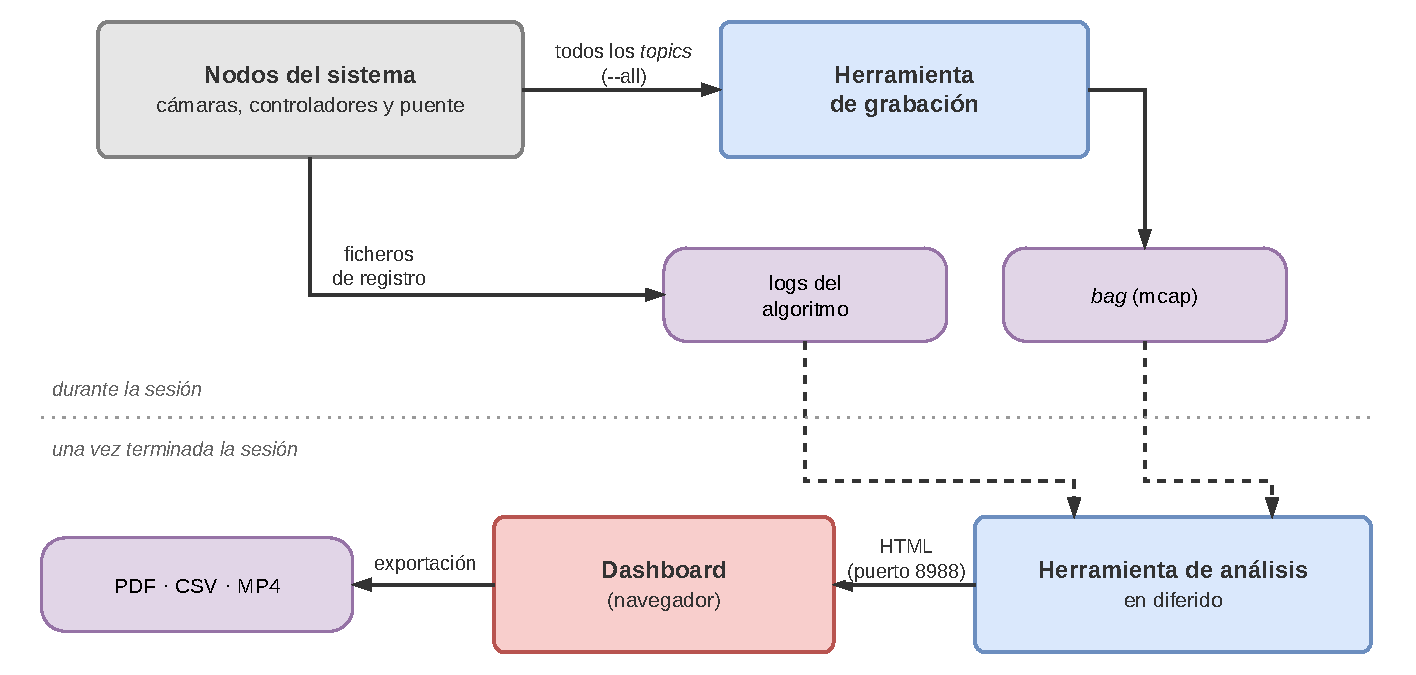
\includegraphics[width=\textwidth]{imaxes/IMPLEMENTACION/flujo_analisis_sistema.pdf}
    \caption{Flujo de datos entre la grabación de la sesión y el análisis en diferido.}
    \label{fig:flujo-visualizacion}
\end{figure}

\subsection{Herramienta de grabación}
\label{subsec:visualizacion-grabacion}

La grabación se construye sobre \emph{rosbag2} (sección~\ref{sec:ros2-rosbag}), empaquetada en un contenedor junto con las definiciones de los mensajes propios, que hay que compilar dentro para poder interpretarlos. Su cometido es capturar sin pérdidas todo el tráfico de la red y dejarlo en disco, sin procesar ni interpretar nada.

La primera versión trabajaba con una lista explícita de \emph{topics}, construida a partir del número de cámaras y de coches configurados, y resultó una fuente constante de errores, porque cada \emph{topic} nuevo o renombrado había que acordarse de reflejarlo en ella. La versión definitiva graba la totalidad de los \emph{topics} y sondea periódicamente en busca de otros, suscribiéndose a los que van apareciendo, con lo que no impone ningún orden de arranque; la calidad de servicio se resuelve igual, adaptando el perfil de cada suscripción al que ofrecen los publicadores que encuentra en lugar de mantener un fichero que reprodujese las políticas del sistema. Se escogió el formato \emph{mcap} porque lleva embebida la definición de cada mensaje, de modo que un \emph{bag} sigue siendo legible aunque las definiciones hayan cambiado desde que se grabó, algo que ocurrió varias veces conforme avanzaba el proyecto.

\subsection{Herramienta de análisis en diferido}
\label{subsec:visualizacion-analisis}

El análisis cruza dos fuentes: la grabación, de la que obtiene todo lo que se publicó en la red, y los ficheros de \emph{log} que escribe el algoritmo, de los que obtiene su estado interno. La primera describe qué hizo el coche y los segundos explican por qué el sistema decidió lo que decidió, de manera que solo cruzándolas puede relacionarse un comportamiento con la decisión que lo provocó.

El resultado es una página web autocontenida con gráficas interactivas, organizada en las secciones que recoge el cuadro~\ref{tab:secciones-dashboard}, desde la que pueden exportarse las gráficas en PDF, los datos en CSV y un vídeo que combina las imágenes de todas las cámaras. Como cada cámara trabaja en sus propias coordenadas de imagen, las gráficas espaciales se dibujan sobre un plano global común aplicando a cada una una traslación fija; este es el único punto del sistema donde las trayectorias de las distintas cámaras se llevan a un mismo plano, y puede hacerse porque queda fuera del lazo de control. La herramienta se ejecuta también en un contenedor, que a diferencia del resto no forma parte del sistema desplegado: se levanta bajo demanda indicándole qué sesión analizar, sirve el \emph{dashboard} en un puerto accesible desde el anfitrión y termina al pararlo. Necesita contenedor por la misma razón que la grabación, porque leer ficheros \emph{mcap} exige tener disponibles las bibliotecas de ROS~2 y las definiciones de los mensajes.

\begin{table}[htbp]
\centering
\resizebox{\textwidth}{!}{
\begin{tabular}{|c|l|}
\hline
\rowcolor{ArqAzulClaro}
\textbf{Sección} & \textbf{Contenido} \\
\hline
0 & Resumen de la sesión \\
\hline
1 & Valor del derrape en cada punto del recorrido (3D) \\
\hline
2 & Trayectorias de las etiquetas delantera y trasera \\
\hline
3 & Distancia de derrape de la etiqueta trasera \\
\hline
4 & Mapa del circuito con el PWM de cada celda \\
\hline
5 & Tiempos por vuelta \\
\hline
6 & Evolución de las zonas, perfil de PWM y resumen por vuelta \\
\hline
7 & Visor de las imágenes grabadas y generación de vídeo \\
\hline
8 & Descarga de los datos en formato CSV \\
\hline
\end{tabular}
}
\caption{Secciones del \emph{dashboard} generado por la herramienta de análisis.}
\label{tab:secciones-dashboard}
\end{table}
 \chapter{Pruebas}
\label{cap:pruebas}

\lettrine{E}{n} este capítulo se recogen las pruebas realizadas sobre el sistema ya montado. La primera cuantifica la diferencia de comportamiento entre los dos coches con una misma configuración. La segunda comprueba, con un PWM que sube solo, hasta dónde aguanta el mismo circuito en días distintos. La tercera ajusta el umbral de derrape del algoritmo y mide qué se gana con ello. La cuarta enfrenta al algoritmo con pilotos humanos, en el óvalo y en el circuito en ocho. La quinta le enfrenta a su propio perfil congelado, para ver si repetir la mejor vuelta que llegó a dar sirve de algo. La sexta mide cuánto retardo añade la red y a partir de qué punto llega a notarse. Las dos últimas llevan el sistema a circuitos grandes con varias cámaras y a una carrera con varios coches.

Todas las gráficas que se muestran proceden de la herramienta de análisis en diferido descrita en la sección~\ref{sec:sistema-visualizacion}.

\section{Prueba comparativa entre coches}
\label{sec:prueba-comparativa-coches}

Para que la única variable fuese el coche se fijó todo lo demás. Se escogió el circuito en óvalo, de tamaño reducido para que quepa entero en el campo de visión de una única cámara. Los tres nodos implicados, el de cámara, el controlador y el puente Arduino, se ejecutaron en la misma máquina, de forma que ni la latencia de red ni el retardo de un paquete pudieran afectar. La configuración fue idéntica en las dos ejecuciones, con un rango de PWM de 70 a 94 y un umbral de derrape de 12~px, y cada coche recorrió 50 vueltas.

La figura~\ref{fig:comparativa-trayectorias} muestra las trayectorias de las dos etiquetas en la vuelta 22. En el coche azul se aprecia en la zona señalada un salto grande entre posiciones consecutivas de la etiqueta trasera, lo que corresponde con un derrape. Mientras que en el coche rojo, con el mismo PWM aplicado, la trasera recorre esa misma curva pegada a la trayectoria base sin llegar a separarse de ella.

\begin{figure}[tbp]
  \centering
  \begin{subfigure}[b]{\textwidth}
    \centering
    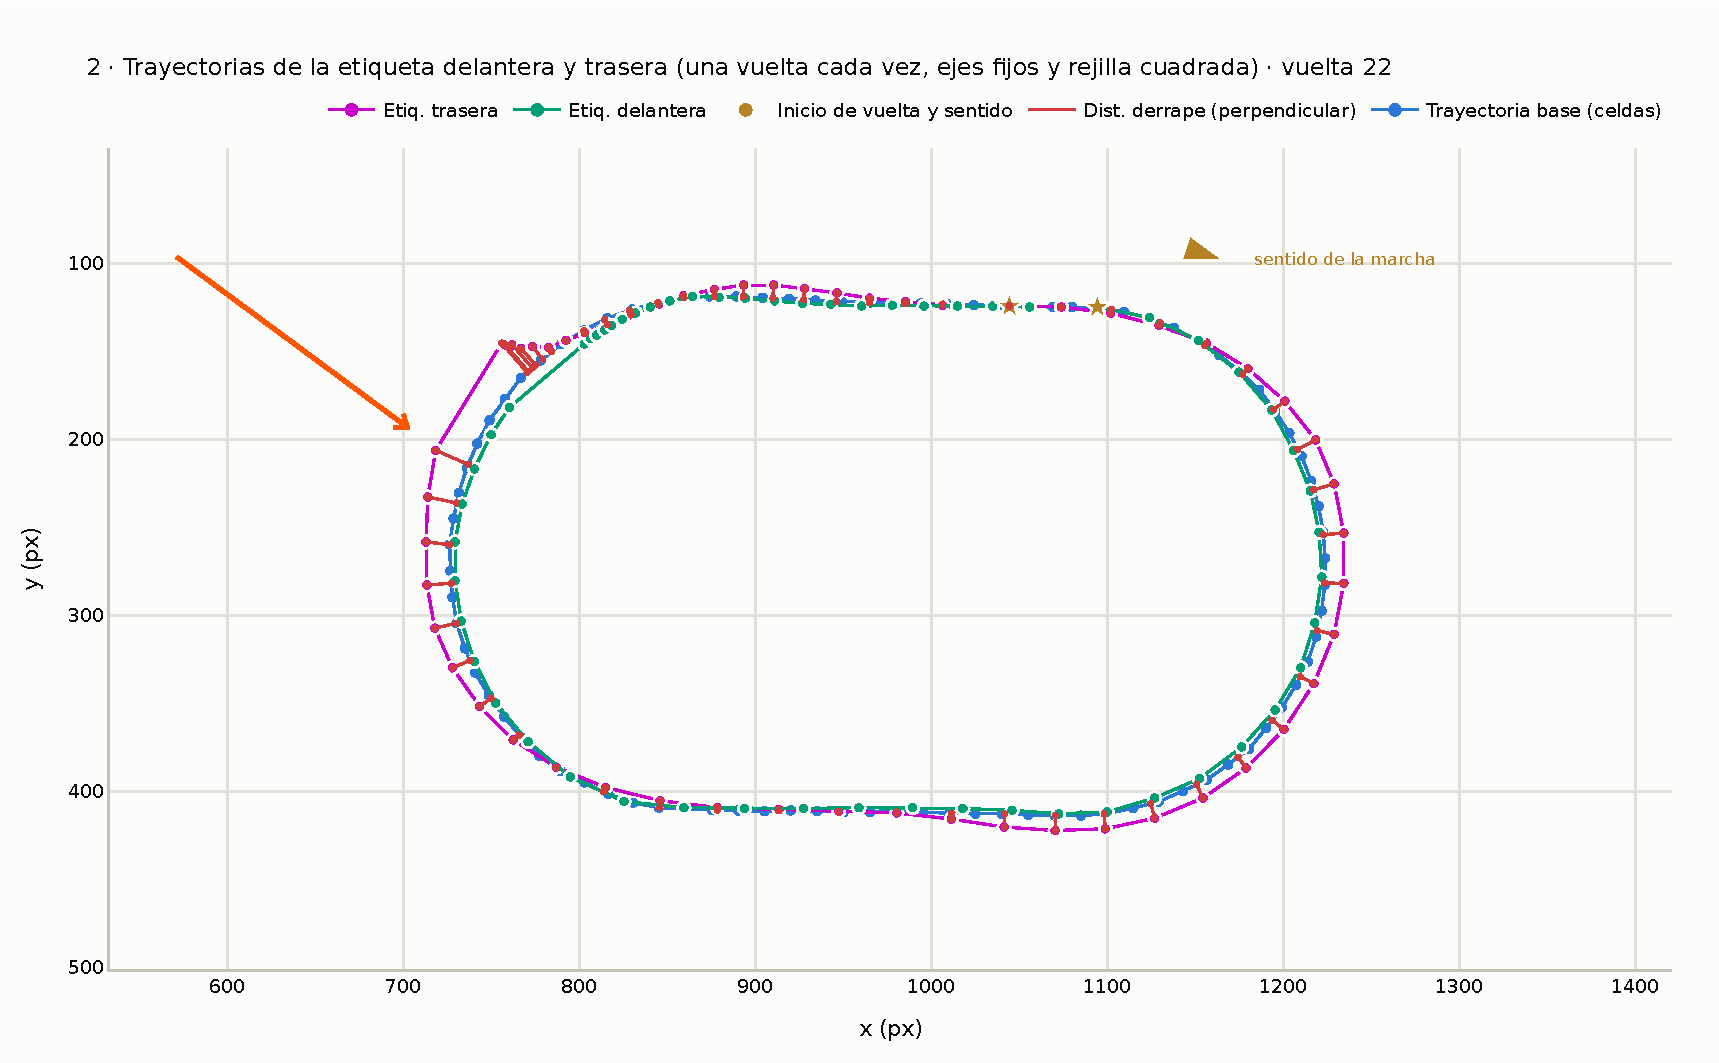
\includegraphics[trim={0 0 0 42pt},clip,width=\linewidth]{imaxes/PRUEBAS/COMPARATIVA_COCHES/dist_derrape_coche_azul.pdf}
    \caption{Coche azul}
    \label{fig:comparativa-trayectorias-azul}
  \end{subfigure}

  \vspace{1em}

  \begin{subfigure}[b]{\textwidth}
    \centering
    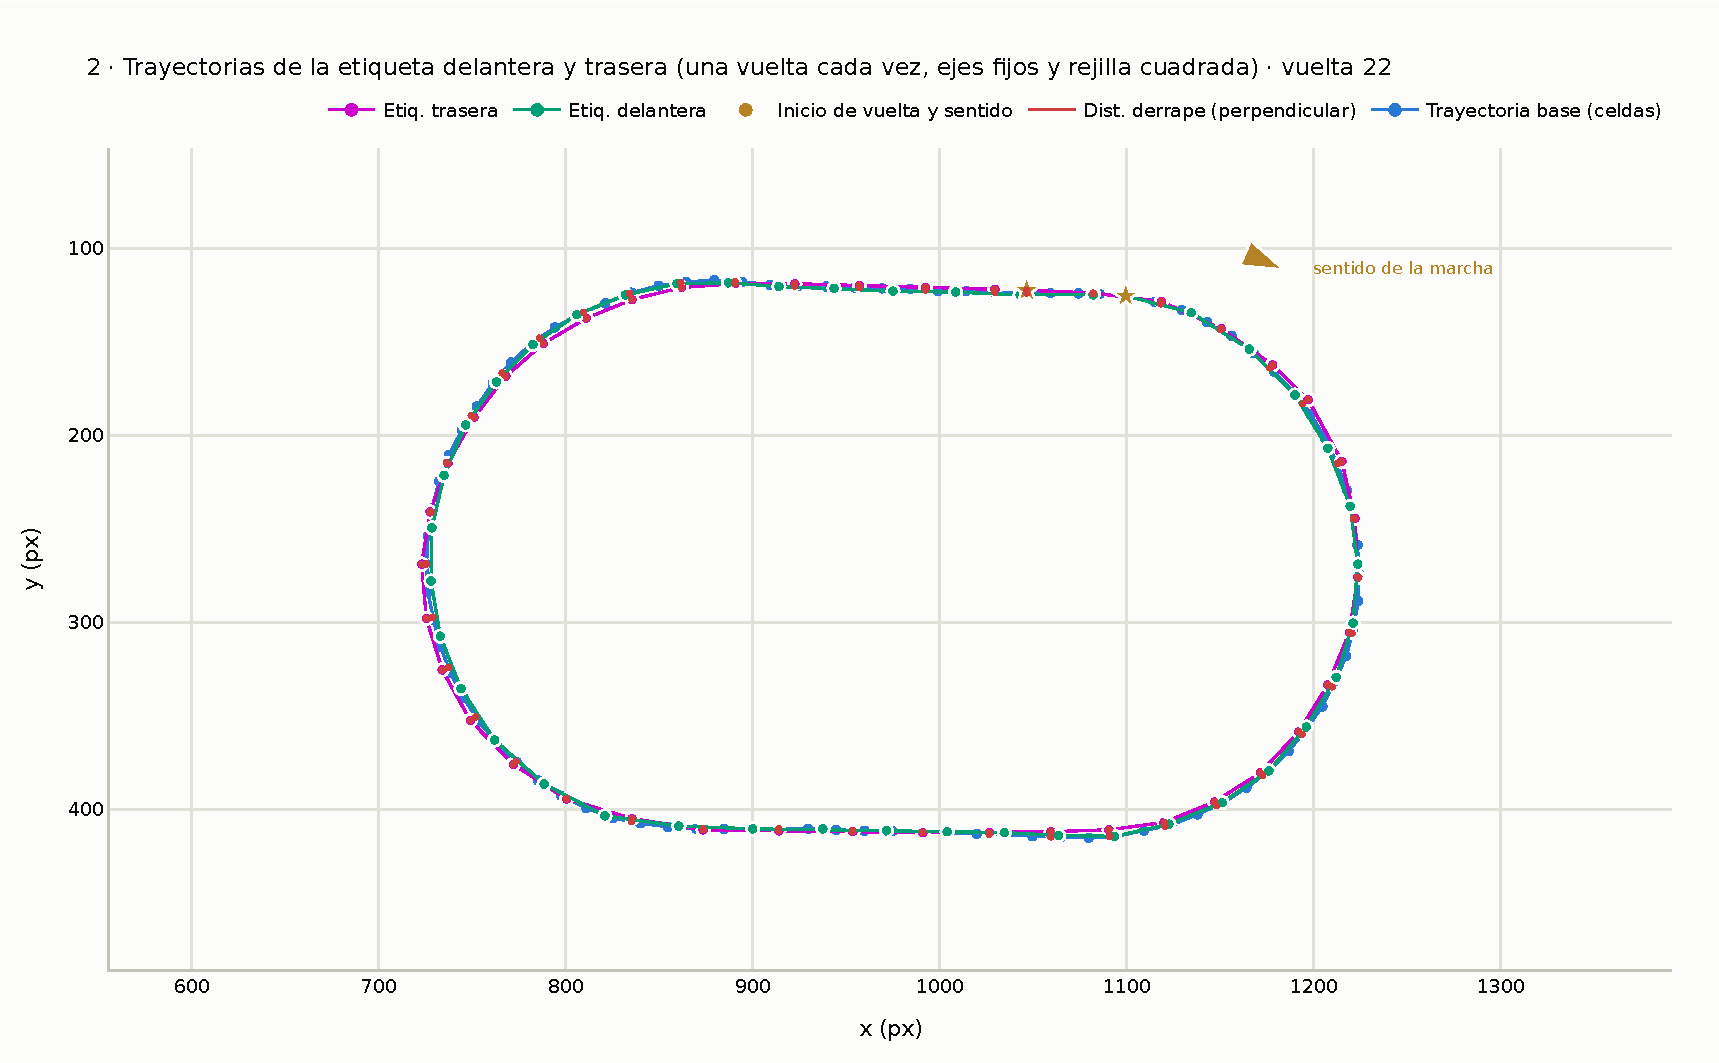
\includegraphics[trim={0 0 0 42pt},clip,width=\linewidth]{imaxes/PRUEBAS/COMPARATIVA_COCHES/dist_derrape_coche_rojo.pdf}
    \caption{Coche rojo}
    \label{fig:comparativa-trayectorias-rojo}
  \end{subfigure}
  \caption{Trayectoria de las dos etiquetas en la vuelta 22 con la misma configuración del algoritmo.}
  \label{fig:comparativa-trayectorias}
\end{figure}

Una vez detectado el derrape el algoritmo castiga al coche azul y genera dos zonas, como se aprecia en la figura~\ref{fig:comparativa-zonas-azul}, la zona de derrape, que cubre las celdas 47 a 68 y queda limitada a PWM 89, y la que ya venía de antes, que se mantiene en 91. En el coche rojo no hubo ningún derrape que castigar y por tanto no se abre ninguna zona nueva, de modo que en la figura~\ref{fig:comparativa-zonas-rojo} sigue habiendo una única zona que además ha continuado subiendo hasta PWM 92.

\begin{figure}[tbp]
  \centering
  \begin{subfigure}[b]{\textwidth}
    \centering
    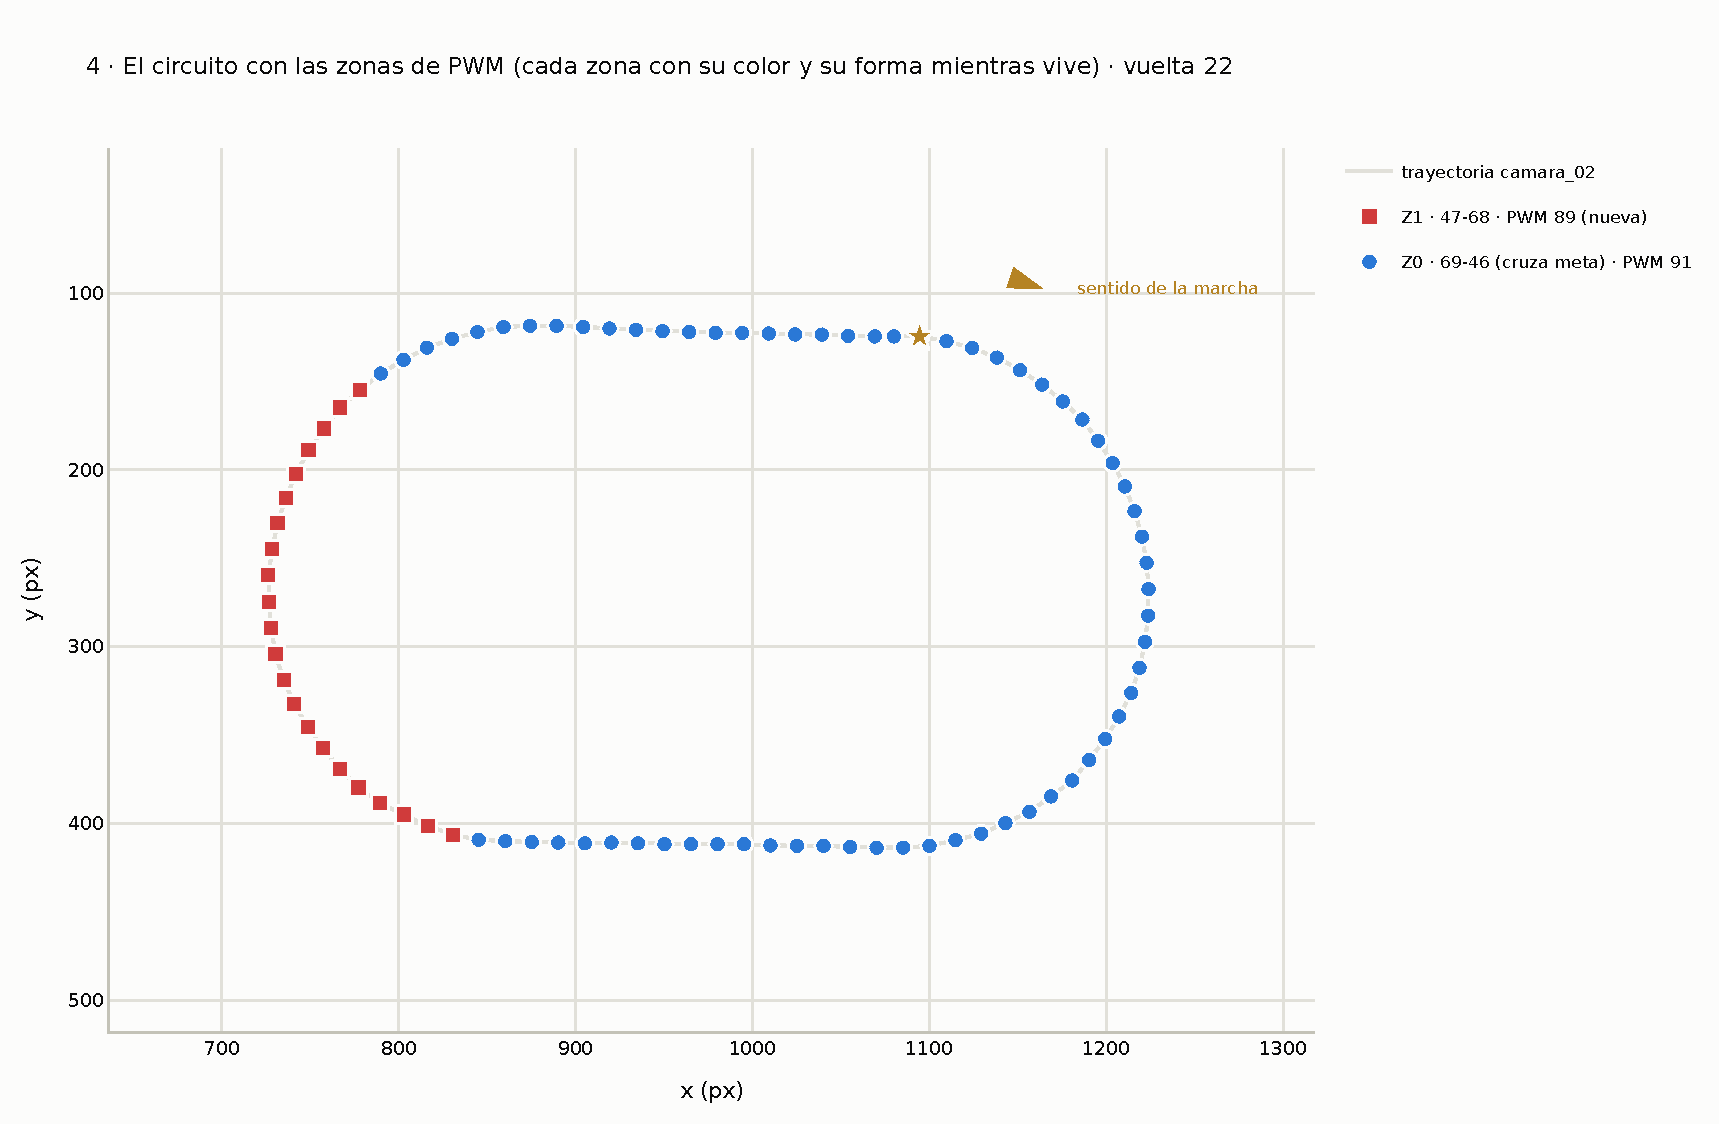
\includegraphics[trim={0 0 0 60pt},clip,page=1,width=\linewidth]{imaxes/PRUEBAS/COMPARATIVA_COCHES/pwm_zonas_coche_azul.pdf}
    \caption{Coche azul}
    \label{fig:comparativa-zonas-azul}
  \end{subfigure}

  \vspace{1em}

  \begin{subfigure}[b]{\textwidth}
    \centering
    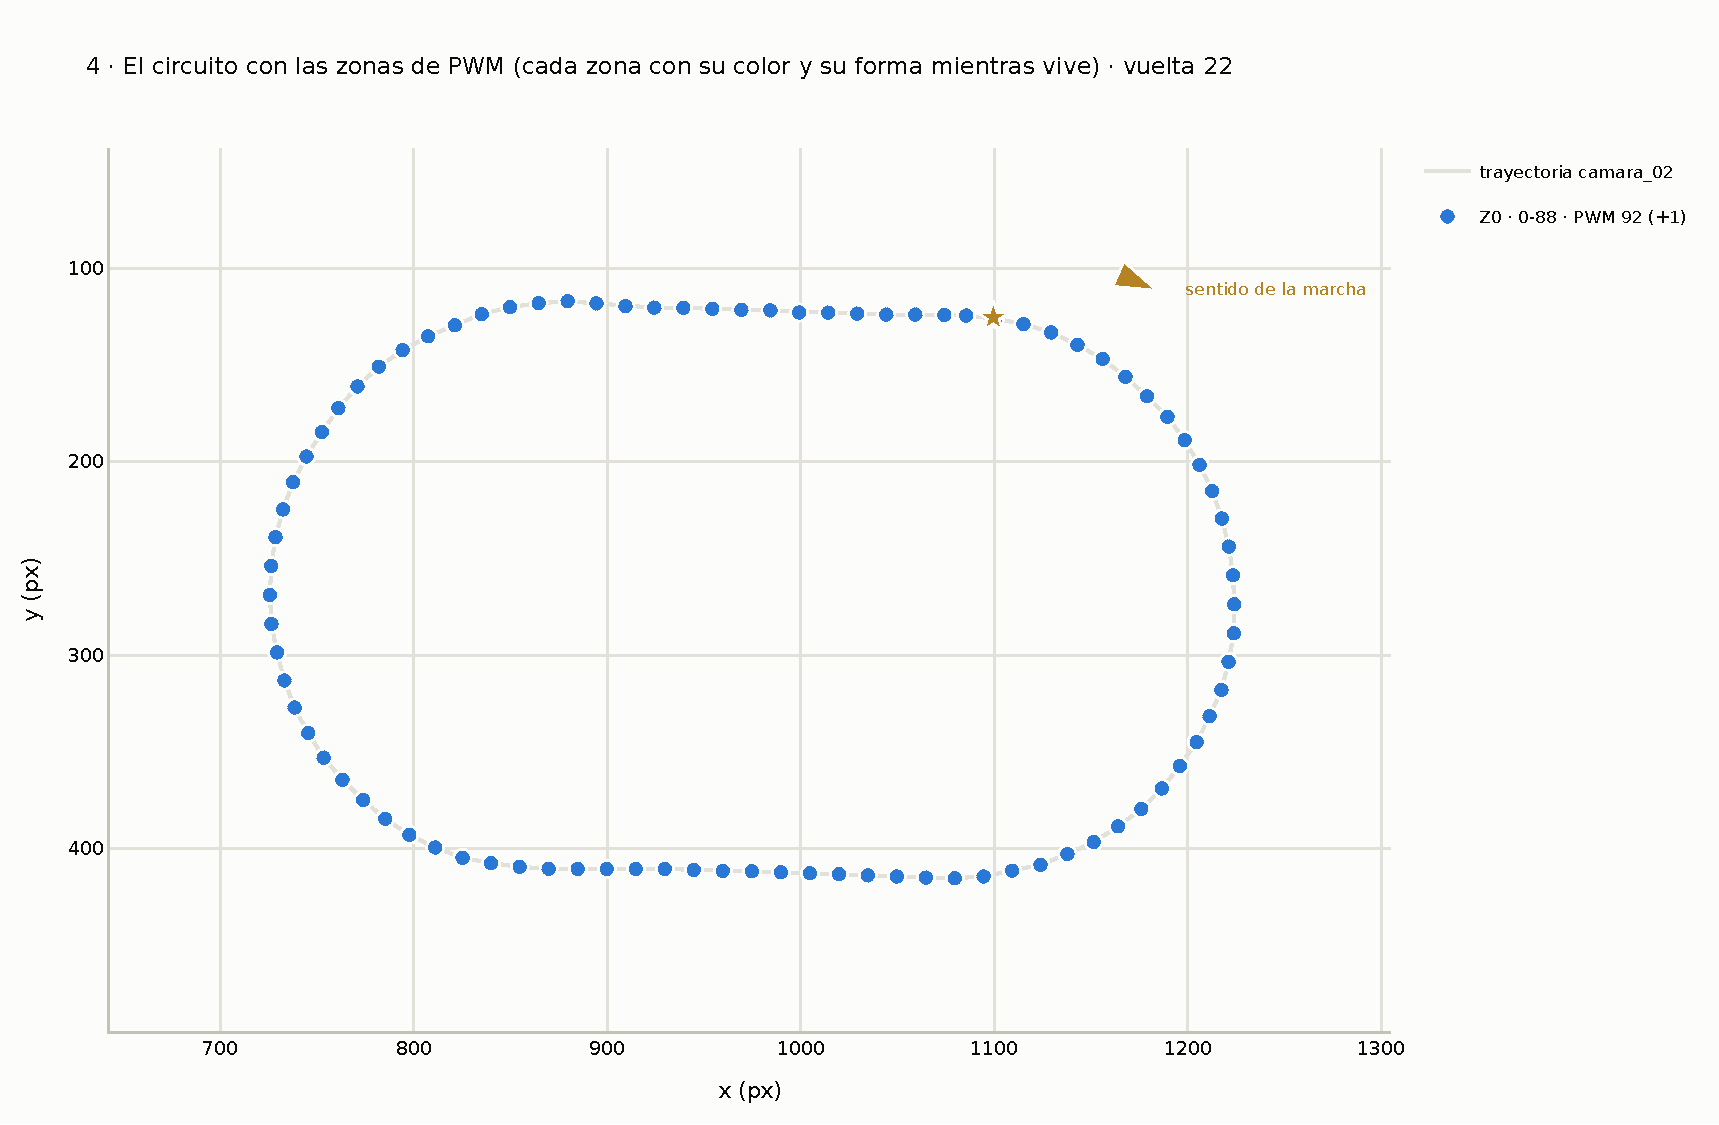
\includegraphics[trim={0 0 0 60pt},clip,page=1,width=\linewidth]{imaxes/PRUEBAS/COMPARATIVA_COCHES/pwm_zonas_coche_rojo.pdf}
    \caption{Coche rojo}
    \label{fig:comparativa-zonas-rojo}
  \end{subfigure}
  \caption{Partición del circuito en zonas de PWM en la vuelta 22. El coche azul arrastra una zona de derrape ya castigada y el rojo mantiene una única zona libre que sigue subiendo.}
  \label{fig:comparativa-zonas}
\end{figure}

El comportamiento no es puntual, sino que se repite a lo largo de toda la ejecución, como recoge la figura~\ref{fig:comparativa-derrapes}, donde se representa vuelta a vuelta la distancia de derrape registrada junto al PWM medio aplicado. El coche azul encadena picos muy por encima del umbral, varios de ellos por encima de los 20~px, que se corresponden con derrapes lo bastante fuertes como para que el coche estuviera a punto de salirse de la pista. En el coche rojo los máximos se mantienen entre los 4 y los 9~px durante toda la carrera y ninguno llega a superar el umbral.

\begin{figure}[tbp]
  \centering
  \begin{subfigure}[b]{\textwidth}
    \centering
    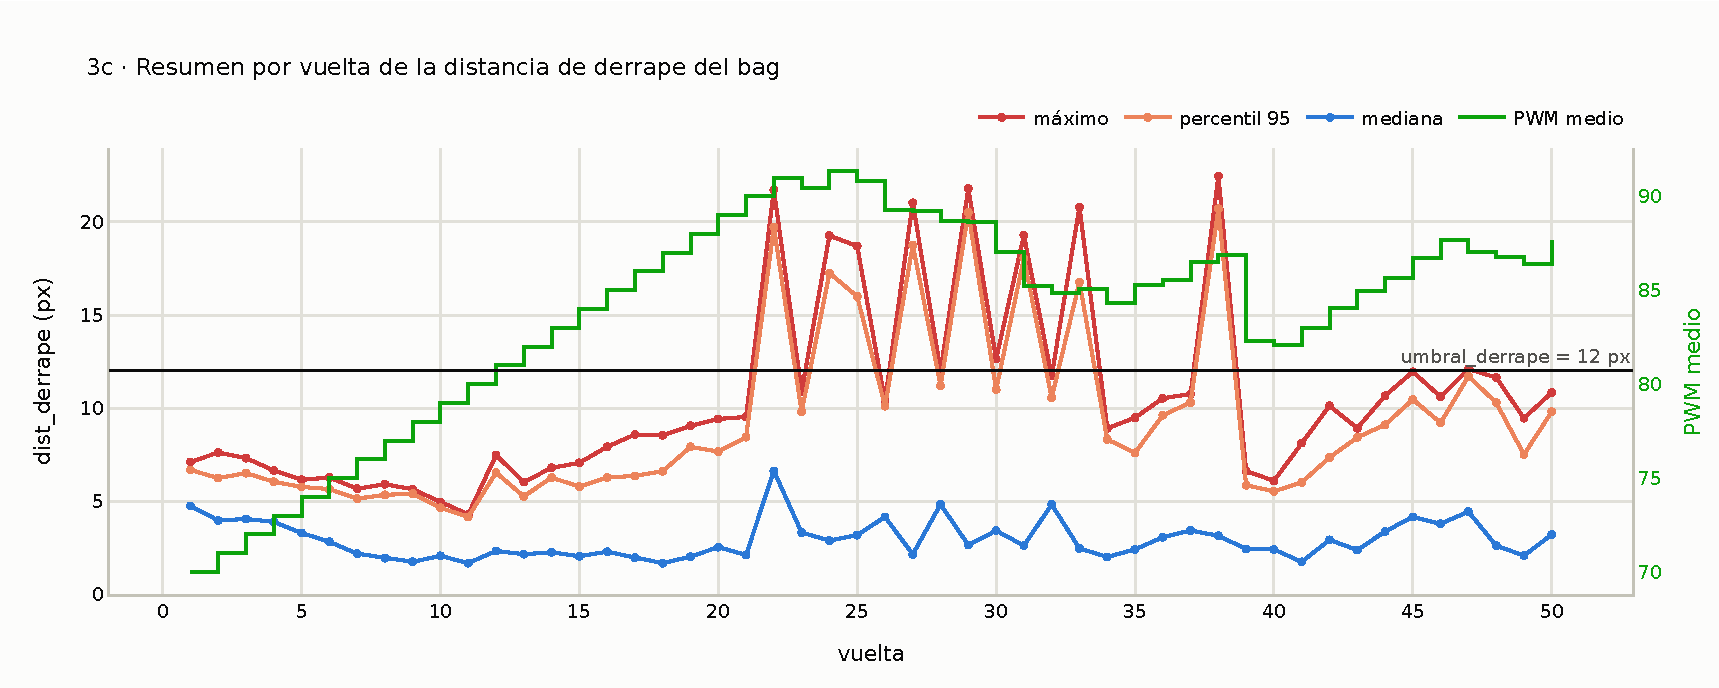
\includegraphics[trim={0 0 0 44pt},clip,width=\linewidth]{imaxes/PRUEBAS/COMPARATIVA_COCHES/resumen_derrapes_coche_azul.pdf}
    \caption{Coche azul}
    \label{fig:comparativa-derrapes-azul}
  \end{subfigure}

  \vspace{1em}

  \begin{subfigure}[b]{\textwidth}
    \centering
    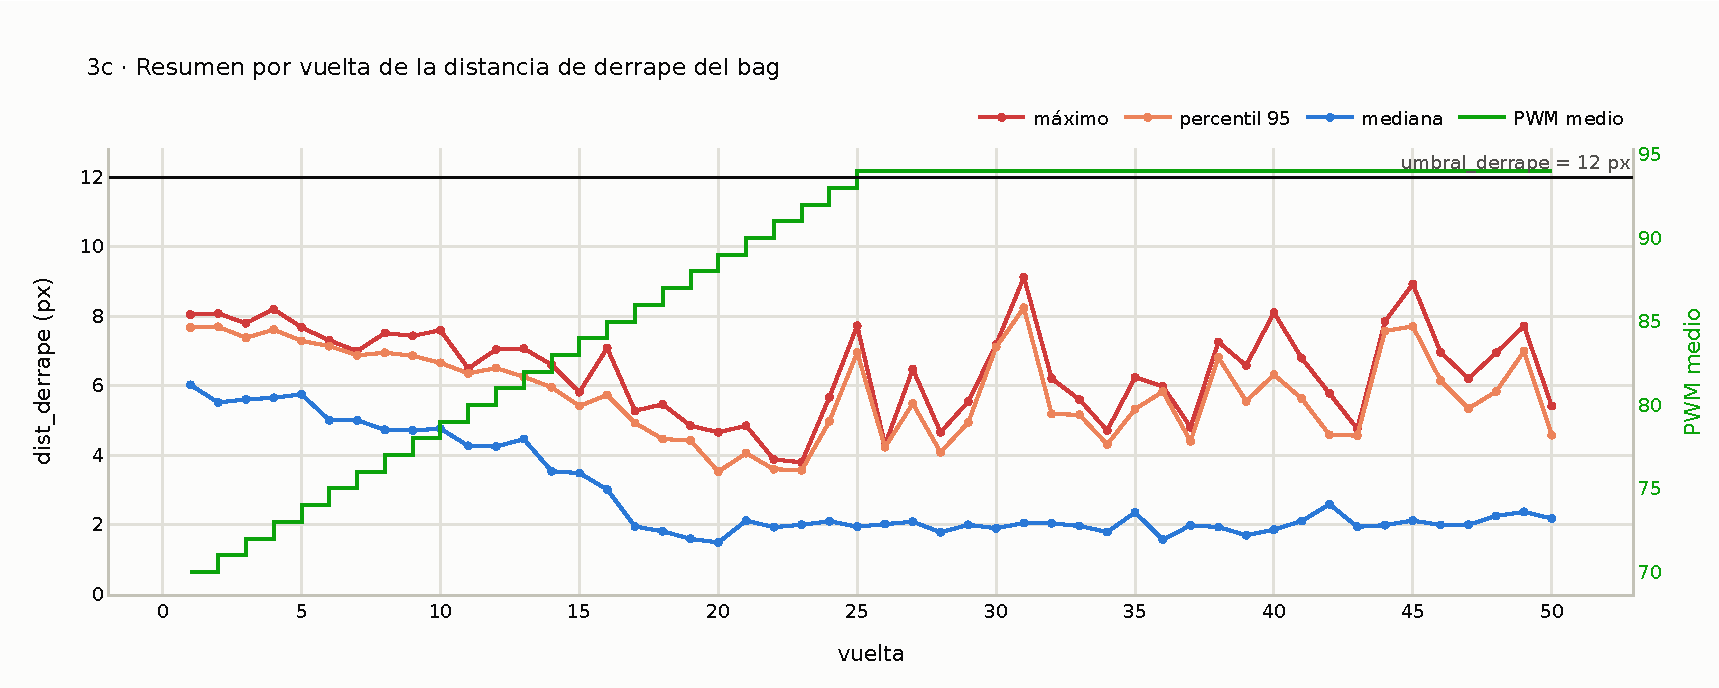
\includegraphics[trim={0 0 0 44pt},clip,width=\linewidth]{imaxes/PRUEBAS/COMPARATIVA_COCHES/resumen_derrapes_coche_rojo.pdf}
    \caption{Coche rojo}
    \label{fig:comparativa-derrapes-rojo}
  \end{subfigure}
  \caption{Resumen por vuelta de cómo varió la distancia de derrape frente al PWM.}
  \label{fig:comparativa-derrapes}
\end{figure}

Los tiempos de las dos ejecuciones, recogidos en la tabla~\ref{tab:comparativa-coches}, confirman lo que muestran las gráficas. El coche rojo tarda 75,44~s en completar las 50 vueltas frente a los 93,59~s del azul, una diferencia de 18~segundos que supone más de un 19\,\% del tiempo total con el mismo algoritmo y la misma configuración. El origen no está en el control, sino en el propio coche, que pierde adherencia con valores de PWM que el rojo asimila sin problema.

\begin{table}[tbp]
  \centering
  \estilotabla[3]
  \caption{Métricas de tiempo por vuelta de ambos coches con la misma configuración (PWM 70--94, umbral de derrape 12~px).}
  \label{tab:comparativa-coches}
  \begin{tabular}{lrrrrr}
    \toprule
    \rowcolor{ArqAzulClaro}
    Coche & Contrarreloj & Mejor & Mediana & Media & $\sigma$ \\
          \rowcolor{ArqAzulClaro} & (s) & (s) & (s) & (s) & (s) \\
    \midrule
    Azul & 93,59 & 1,661 & 1,755 & 1,872 & 0,228 \\
    Rojo & 75,44 & 1,315 & 1,377 & 1,509 & 0,232 \\
    \bottomrule
  \end{tabular}
\end{table}

El problema no afecta solo al algoritmo, porque en las pruebas de conducción manual de la sección~\ref{sec:prueba-algo-vs-personas} a las personas también les cuesta más controlar el coche azul, ya que es mucho más sensible a los valores altos de PWM. La consecuencia práctica de todo esto es que no existe una configuración única válida para los dos coches y que los parámetros del algoritmo, en particular el umbral de derrape, deben ajustarse a las características del vehículo, que es lo que se comprueba en la prueba~\ref{sec:prueba-algo-parametros}.

\section{Prueba PWM incremental}
\label{sec:prueba_pwm_incremental}

Durante las pruebas unitarias aparecieron problemas en el comportamiento del circuito, los valores y las configuraciones que servían un día para un coche ya no eran valían al día siguiente. Igual que en la prueba anterior, todos los nodos se lanzaron en un mismo ordenador para que la red no influyera en el control del coche, y para ver el comportamiento para un PWM se aplico el modo incremental, descrito en la sección~\ref{subsec:modos-operacion}, aumentado el valor cada 10 vueltas. Se realizaron seis ejecuciones que recogidas en la tabla~\ref{tab:incremental-sesiones}, se usaron los dos coches y en dos días distintos.

\begin{table}[tbp]
  \centering
  \estilotabla[3]
  \caption{Resumen ejecuciones de la prueba con PWM incremental.}
  \label{tab:incremental-sesiones}
  \begin{tabular}{llcrcrc}
    \toprule
    \rowcolor{ArqAzulClaro}
    Coche & Día & Sesión & Vueltas & PWM & Mejor & Sin mejora \\
          \rowcolor{ArqAzulClaro} & & & & & (s) & desde PWM \\
    \midrule
    Azul & 22/07 & 001 & 243 & 70--93  & 1,697 & 74 \\
    Azul & 22/07 & 002 & 236 & 70--92  & 1,702 & 85 \\
    Azul & 03/09 & ---  & 361 & 75--110 & 1,863 & 92 \\
    Rojo & 22/07 & 001 & 277 & 70--95  & 1,581 & 93 \\
    Rojo & 22/07 & 002 & 261 & 70--95  & 1,584 & 93 \\
    Rojo & 03/09 & ---  & 360 & 75--110 & 1,350 & 98 \\
    \bottomrule
  \end{tabular}
\end{table}

Con el coche azul, el 22/07 una vuelta se daba en 1,774~s con un PWM de 75, mientras que el 03/09 ese mismo valor necesitaba 3,095~s y hubo que llegar hasta 110 para acercarse al tiempo que el otro día se conseguía con 74. Con el coche rojo ocurre justo lo contrario, porque el 03/09 fue más rápido que el 22/07 en todos los valores comunes, entre 0,15 y 0,53~s por vuelta. Los números están en la tabla~\ref{tab:incremental-por-pwm}. Destacar que la distancia de derrape se mantiene en valores parecidos entre las sesiones, alrededor de 5~px el azul y de 9~px el rojo. 

\begin{table}[tbp]
  \centering
  \estilotabla[3]
  \caption{Tiempo por vuelta ($t$, mediana del escalón) y distancia de derrape ($d$, percentil 95) en los valores de PWM comunes a los dos días. Se usan las sesiones 001 del 22/07.}
  \label{tab:incremental-por-pwm}
  \begin{tabular}{lrrrrrrrr}
    \toprule
    \rowcolor{ArqAzulClaro}
    & \multicolumn{2}{c}{Azul 22/07} & \multicolumn{2}{c}{Azul 03/09}
    & \multicolumn{2}{c}{Rojo 22/07} & \multicolumn{2}{c}{Rojo 03/09} \\
    \rowcolor{ArqAzulClaro}
    PWM & $t$ (s) & $d$ (px) & $t$ (s) & $d$ (px)
        & $t$ (s) & $d$ (px) & $t$ (s) & $d$ (px) \\
    \midrule
    75 & 1,774 & 4,9 & 3,095 & 5,7 & 2,351 & 8,8 & 1,825 & 10,8 \\
    80 & 1,781 & 5,1 & 2,457 & 5,1 & 2,167 & 8,2 & 1,596 & 9,8 \\
    85 & 1,774 & 5,7 & 2,226 & 4,4 & 1,911 & 8,0 & 1,515 & 9,2 \\
    90 & 1,763 & 6,1 & 2,029 & 5,2 & 1,737 & 7,1 & 1,510 & 9,1 \\
    93 & 1,767 & 6,2 & 1,954 & 6,2 & 1,633 & 6,6 & 1,480 & 8,7 \\
    \bottomrule
  \end{tabular}
\end{table}

Apartir de los resultados obtenidos tambin se aprecia que pasado cierto punto subir el PWM deja de mejorar el tiempo. La figura~\ref{fig:incremental-escalera} lo enseña el coche azul del 22/07 baja de 2,00 a 1,78~s entre los valores 70 y 74, y ahí se queda clavado, de manera que los diecinueve escalones que vienen después, hasta el 93, no tienen gran impacto en el tiempo. El del 03/09 sigue mejorando un poco más, hasta el 92, y a partir de ahí se estanca igual. El problema, por tanto, no es solo que haya que aplicar un PWM mayor, sino que ni aplicándolo se recuperan los tiempos de otros dias. Y al forzar el valor por arriba es cuando el coche acaba saliéndose, ya que el último escalón del 03/09 es el único de toda la prueba en el que el azul llega a descontrolarse, con vueltas de 2,8~s y separaciones de la trayectoria de hasta 37~px.

\begin{figure}[tbp]
  \centering
  \begin{subfigure}[b]{0.85\textwidth}
    \centering
    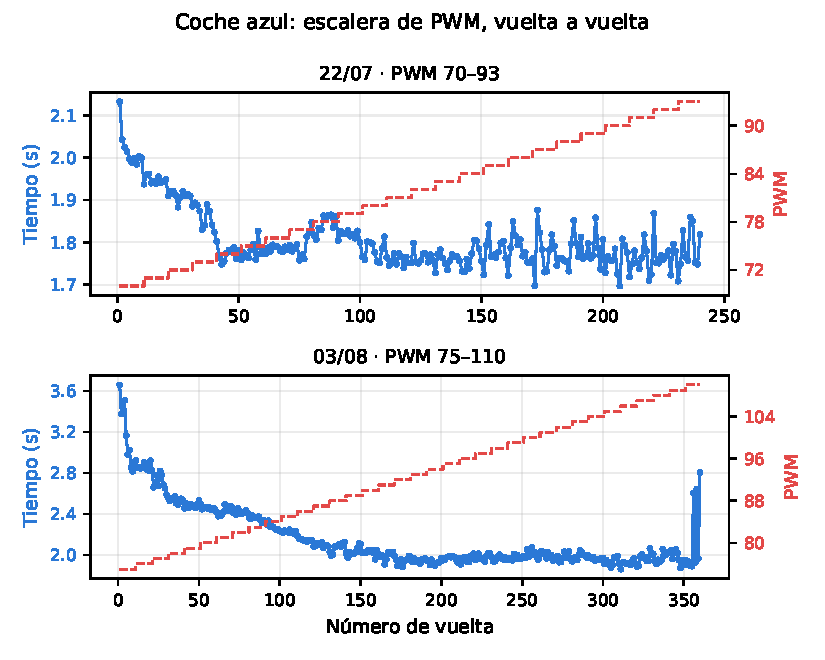
\includegraphics[trim={0 0 0 24},clip,width=\linewidth]{imaxes/PRUEBAS/PWM_INCREMENTAL/escalera_azul.pdf}
    \caption{Coche azul}
    \label{fig:incremental-escalera-azul}
  \end{subfigure}

  \vspace{0.5em}

  \begin{subfigure}[b]{0.85\textwidth}
    \centering
    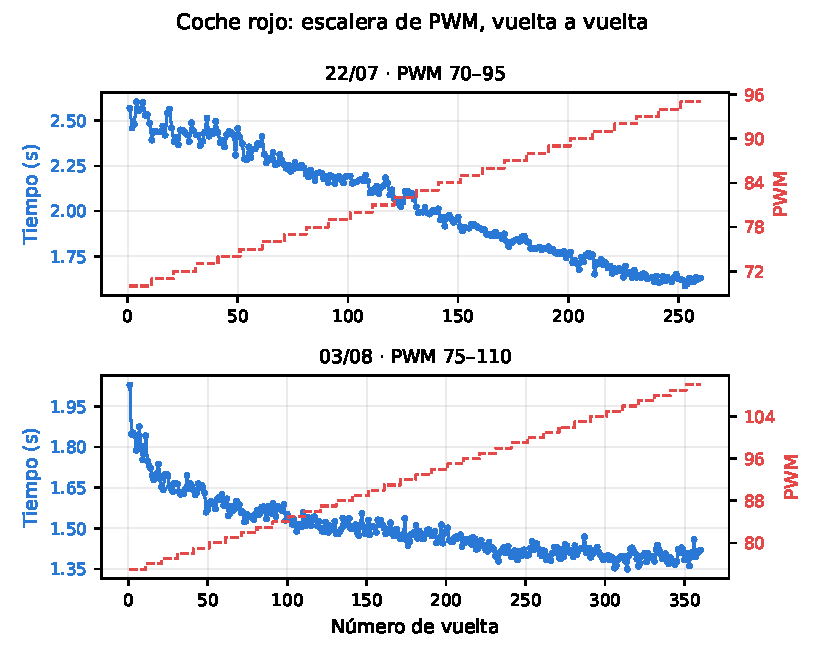
\includegraphics[trim={0 0 0 24},clip,width=\linewidth]{imaxes/PRUEBAS/PWM_INCREMENTAL/escalera_rojo.pdf}
    \caption{Coche rojo}
    \label{fig:incremental-escalera-rojo}
  \end{subfigure}
  \caption{Tiempo por vuelta y escalera de PWM de las dos sesiones de cada coche.}
  \label{fig:incremental-escalera}
\end{figure}

La causa más probable de estos problemas sea el propio montaje de la pista, que exige un buen contacto entre los carriles y que además se monta con piezas mezcladas de varios modelos de Scalextric, de manera que el comportamiento del coche no siempre es el esperado y resulta difícil predecirlo de un día para otro. Esto obliga a tener cuidado al cargar una política ya fijada, porque puede funcionar un día y dejar de hacerlo en otro. Con el algoritmo el problema se puede sortear, ya que basta con relanzarlo o cambiar sus parámetros en caliente, pero no deja de ser un apaño y es una de las limitaciones que se le detectaron, porque no llega a adaptarse por sí solo al comportamiento del circuito. Un algoritmo suficientemente bueno subiría su propio techo de PWM al ver que el circuito no responde, y eso no se contempló durante el diseño porque no se esperaba este comportamiento, que en los trabajos anteriores no aparece reportado.

\section{Prueba de ajuste de los parámetros del algoritmo}
\label{sec:prueba-algo-parametros}

El parámetro sobre el que tiene sentido actuar es el umbral de derrape, que determina a partir de qué separación de la etiqueta trasera respecto a la trayectoria base se considera que el coche está derrapando. Se reprodujeron las mismas condiciones de la sección~\ref{sec:prueba-comparativa-coches}, con el circuito en óvalo cubierto por una sola cámara, todos los nodos en la misma máquina y 50 vueltas por ejecución, y se realizaron tres ejecuciones con el coche azul variando el techo de PWM y el umbral.

La figura~\ref{fig:parametros-tiempos} compara la evolución del tiempo por vuelta con los dos umbrales. Con 9~px el algoritmo detecta los derrapes antes de que empiecen a ser problemáticos (los que se producen cuando el coche empieza a coger velocidad y a ganar inercia), y baja la potencia del carril antes de que el derrape llegue a manifestarse, con lo que la curva se estabiliza a partir de la vuelta 12 y el peor tiempo queda en las primeras vueltas. Con 12~px aparecen entre las vueltas 21 y 38 los picos señalados en la gráfica, que se corresponden con derrapes como el de la figura~\ref{fig:comparativa-trayectorias-azul} y en los que el coche llega casi a salirse de la pista y necesita varias vueltas para recuperar el ritmo, de manera que se vuelve prácticamente a los tiempos que teníamos antes de empezar la carrera.

\begin{figure}[tbp]
  \centering
  \begin{subfigure}[b]{\textwidth}
    \centering
    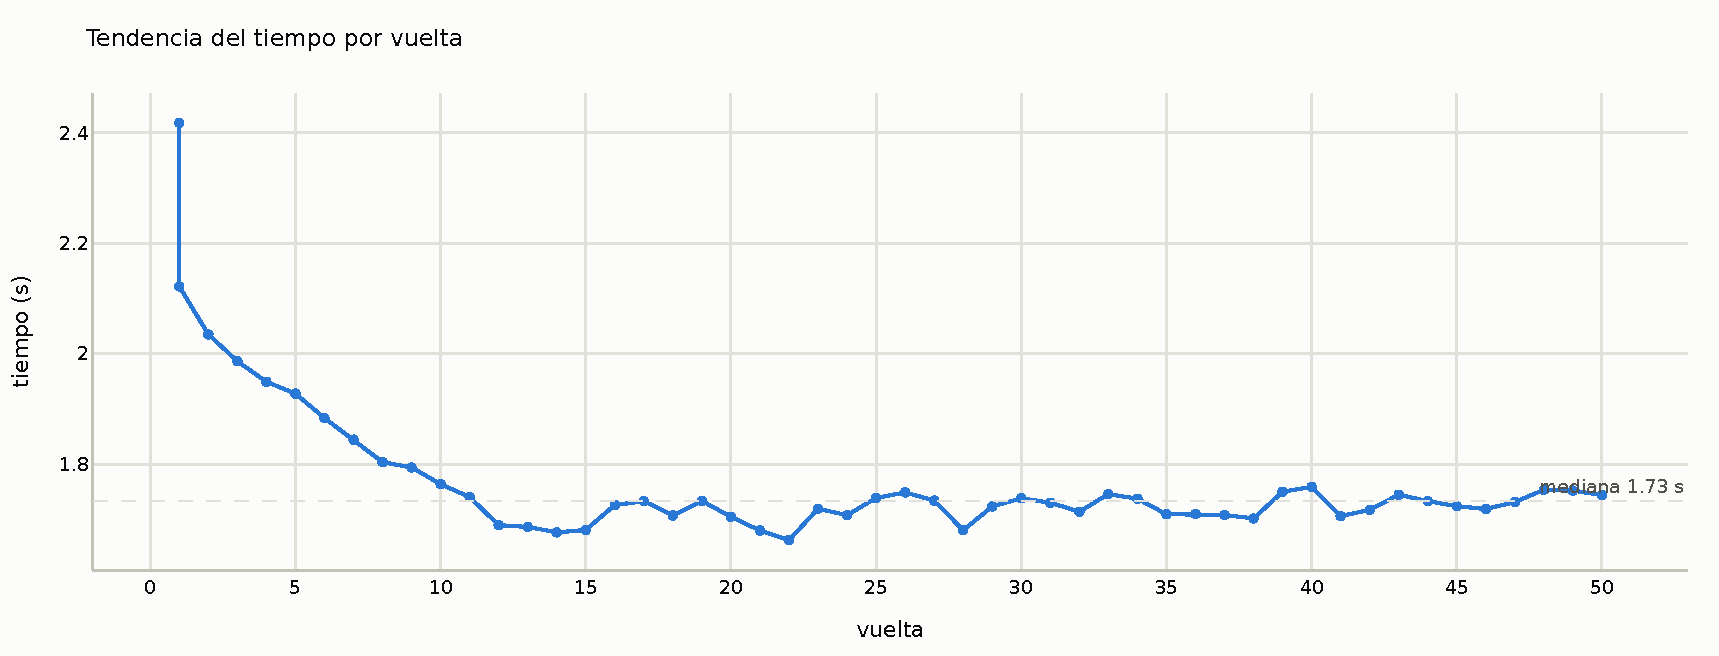
\includegraphics[trim={0 0 0 38pt},clip,width=\linewidth]{imaxes/PRUEBAS/ALGO_VARIOS_PARAMETROS/tiempos_vuelta_mejora_azul.pdf}
    \caption{Umbral de derrape 9~px}
    \label{fig:parametros-tiempos-mejor}
  \end{subfigure}

  \vspace{1em}

  \begin{subfigure}[b]{\textwidth}
    \centering
    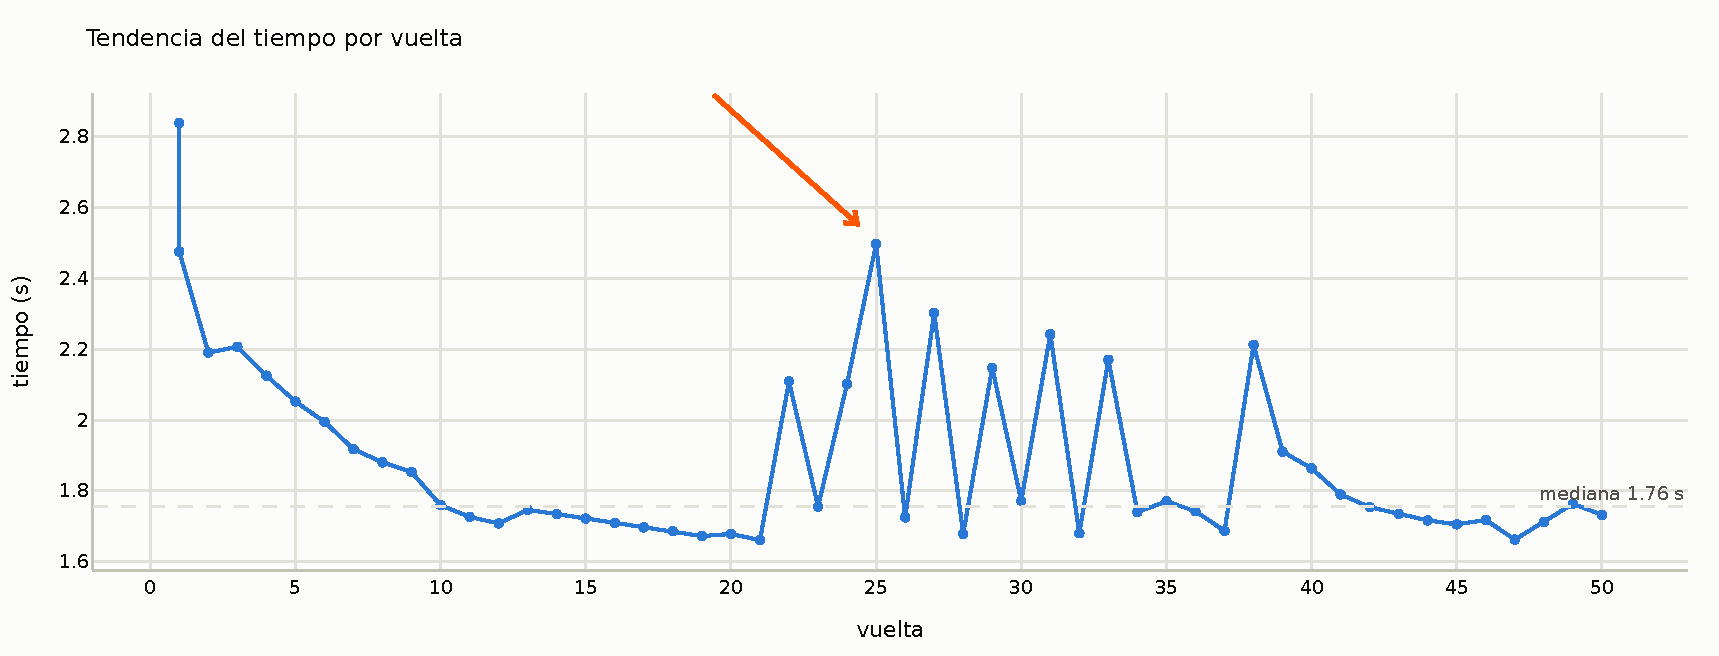
\includegraphics[trim={0 0 0 38pt},clip,width=\linewidth]{imaxes/PRUEBAS/ALGO_VARIOS_PARAMETROS/tiempos_vuelta_peor_azul.pdf}
    \caption{Umbral de derrape 12~px}
    \label{fig:parametros-tiempos-peor}
  \end{subfigure}
  \caption{Evolución del tiempo por vuelta del coche azul en el circuito en óvalo con PWM 70--94 y dos umbrales de derrape distintos.}
  \label{fig:parametros-tiempos}
\end{figure}

La razón de esos picos se ve en la figura~\ref{fig:parametros-derrapes}. Con el umbral en 9~px los derrapes siguen produciéndose, pero se mantienen acotados alrededor de esa misma cifra y solo en unas pocas vueltas llegan a los 10~px, mientras que con el umbral en 12~px el sistema no reacciona hasta que el derrape ya está desarrollado y para entonces el castigo llega tarde, con máximos que se disparan por encima de los 20~px. Ese contraste se aprecia mejor en la figura~\ref{fig:derrape-vuelta}. Con el umbral en 9~px el derrape se detecta mientras todavía está creciendo y el pico se queda en los 10~px, mientras que con 12~px se produce un salto de esa misma franja hasta los 19~px sin ningún paso intermedio. La nube de puntos grises del fondo, que acumula todas las vueltas de la ejecución, se concentra justo entre los 9 y los 10~px, de manera que ahí está la frontera y una vez superada el derrape ya no se puede contener.

\begin{figure}[tbp]
  \centering
  \begin{subfigure}[b]{\textwidth}
    \centering
    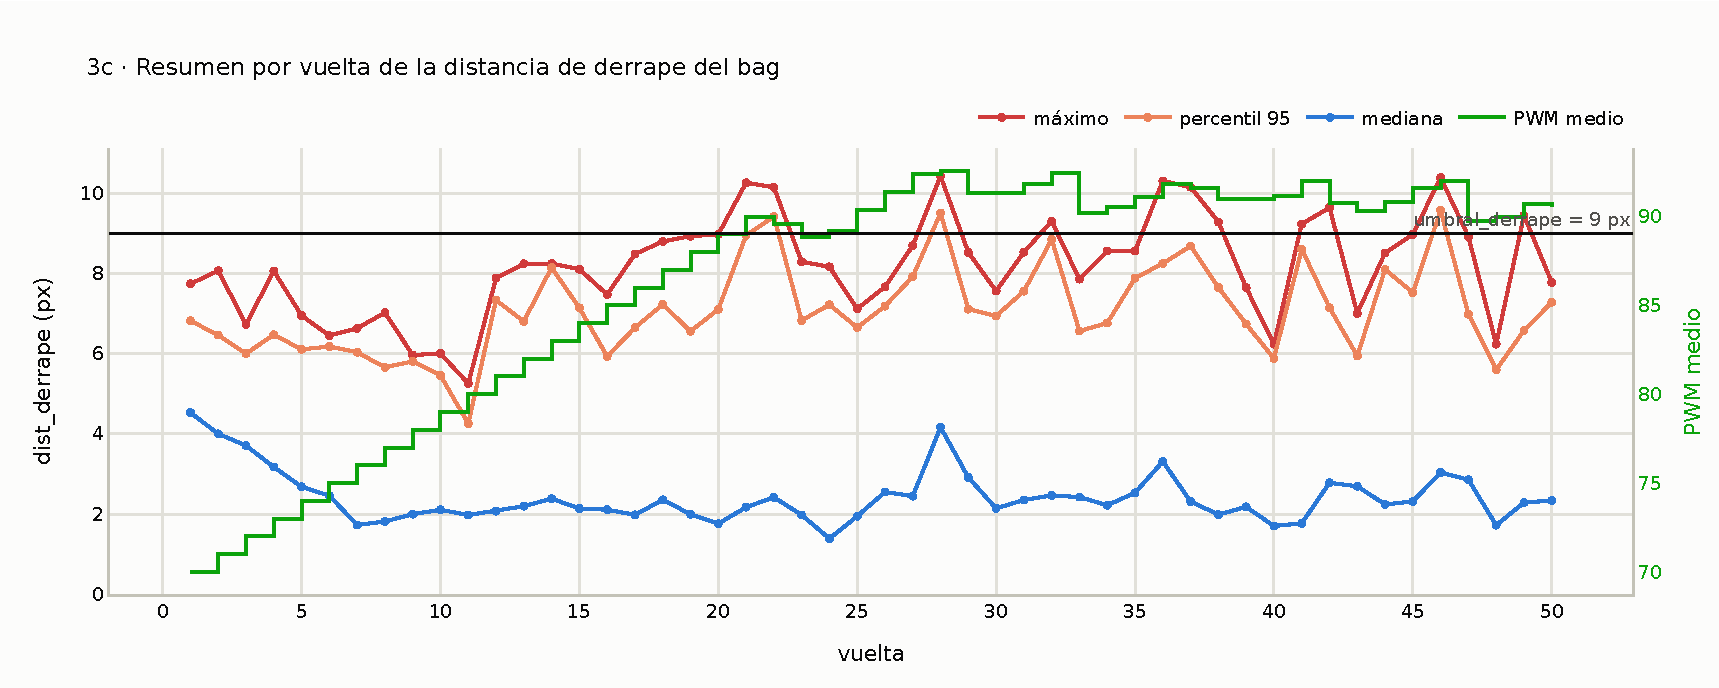
\includegraphics[trim={0 0 0 44pt},clip,width=\linewidth]{imaxes/PRUEBAS/ALGO_VARIOS_PARAMETROS/resumen_dist_derrapes_mejora_azul.pdf}
    \caption{Umbral de derrape 9~px}
    \label{fig:parametros-derrapes-mejor}
  \end{subfigure}

  \vspace{1em}

  \begin{subfigure}[b]{\textwidth}
    \centering
    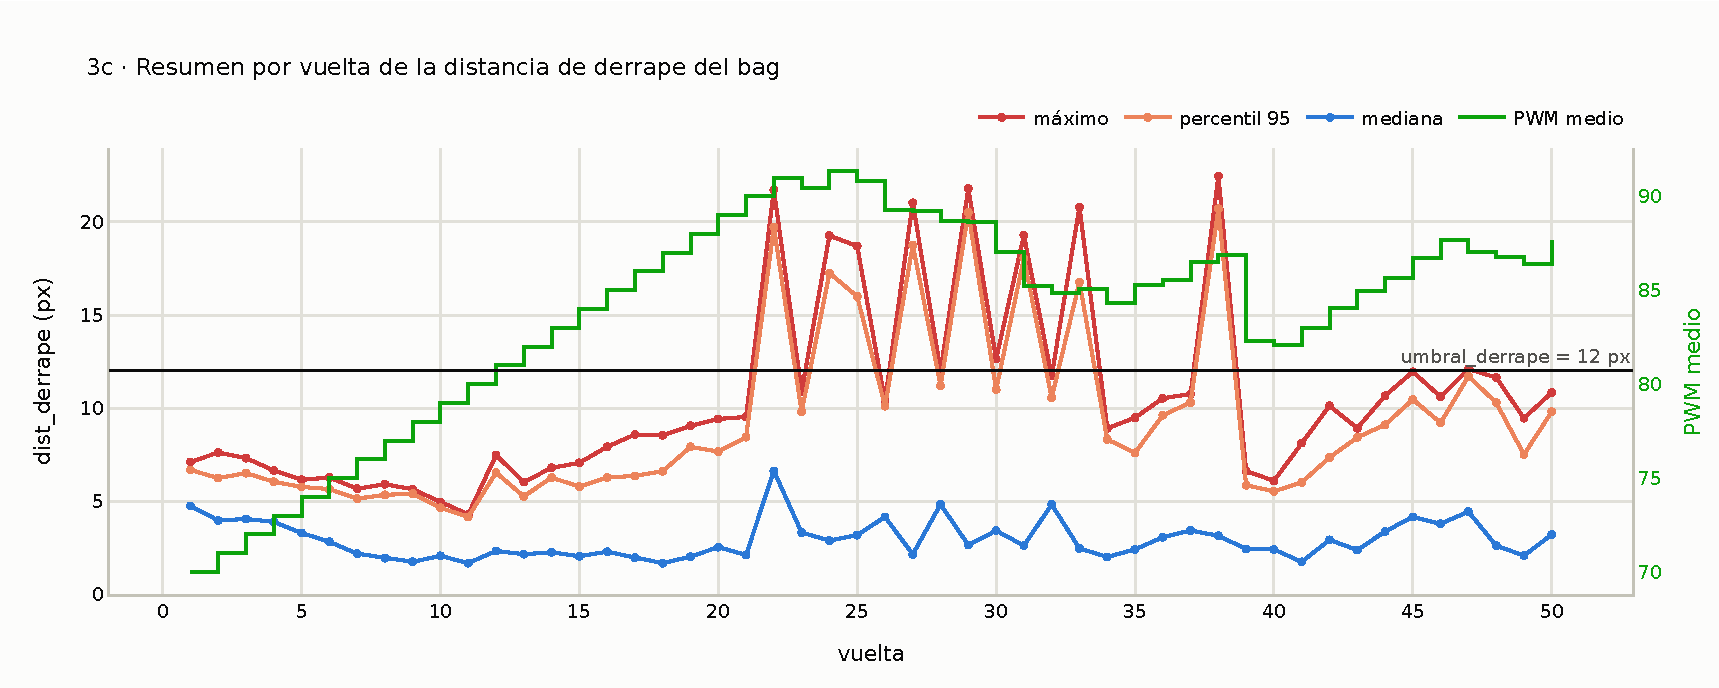
\includegraphics[trim={0 0 0 44pt},clip,width=\linewidth]{imaxes/PRUEBAS/ALGO_VARIOS_PARAMETROS/resumen_dist_derrapes_peor_azul.pdf}
    \caption{Umbral de derrape 12~px}
    \label{fig:parametros-derrapes-peor}
  \end{subfigure}
  \caption{Resumen por vuelta de la distancia de derrape del coche azul con los dos umbrales.}
  \label{fig:parametros-derrapes}
\end{figure}

\begin{figure}[tbp]
  \centering
  \begin{subfigure}[b]{\textwidth}
    \centering
    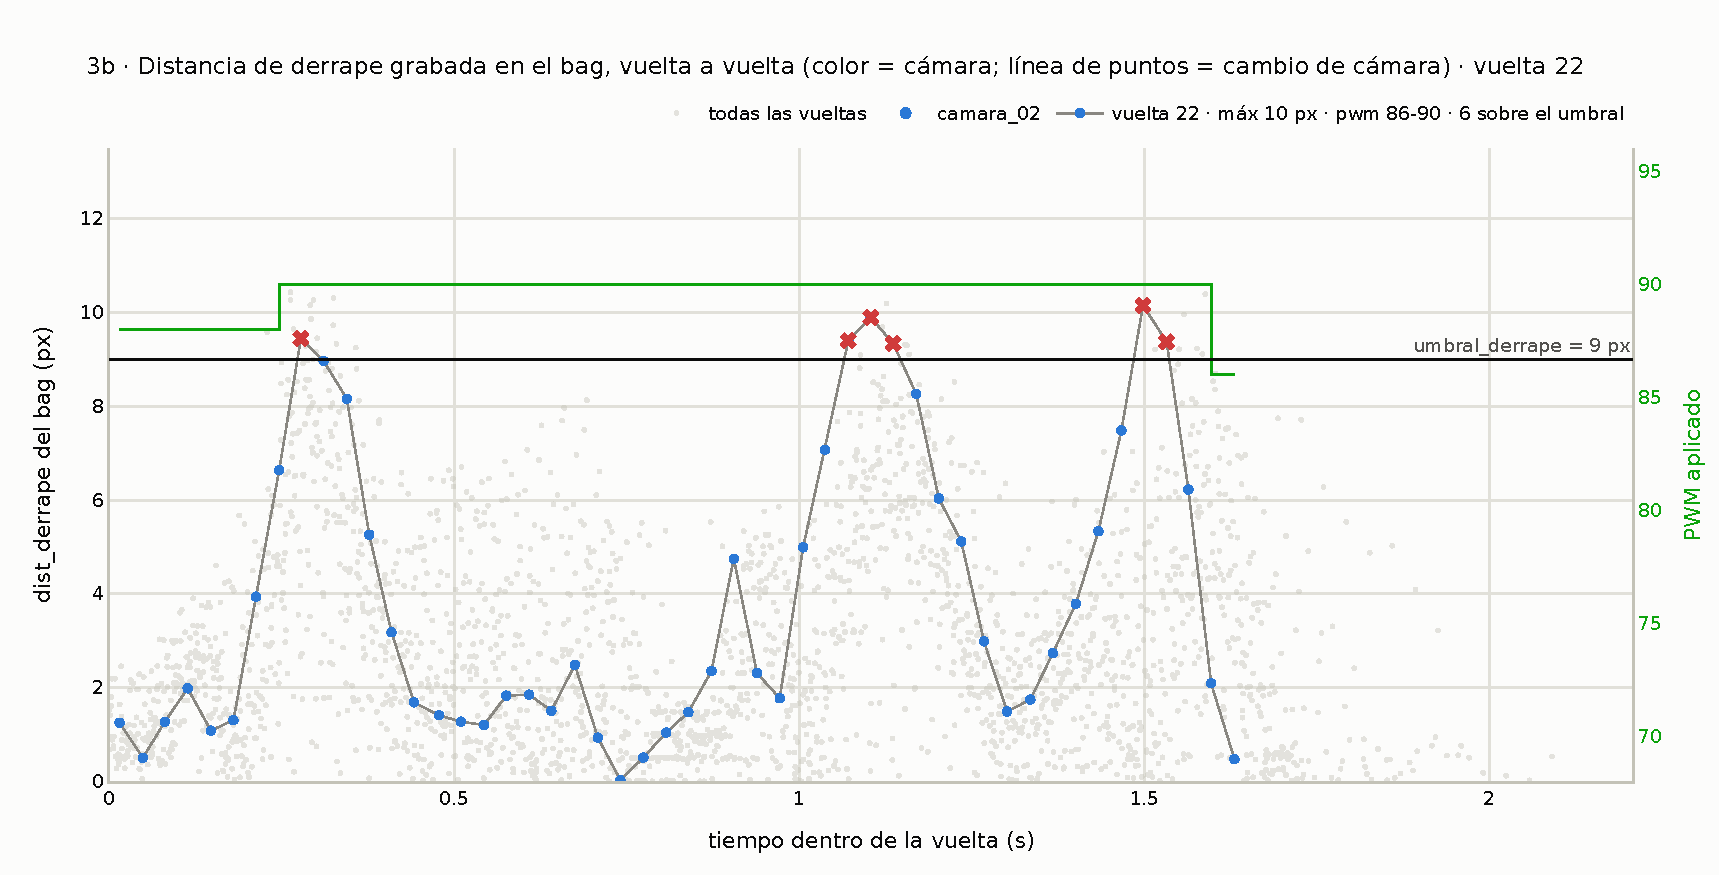
\includegraphics[trim={0 0 0 43pt},clip,width=\linewidth]{imaxes/PRUEBAS/ALGO_VARIOS_PARAMETROS/derrape_controlado.pdf}
    \caption{Umbral de derrape 9~px, vuelta 22}
    \label{fig:derrape-controlado}
  \end{subfigure}

  \vspace{1em}

  \begin{subfigure}[b]{\textwidth}
    \centering
    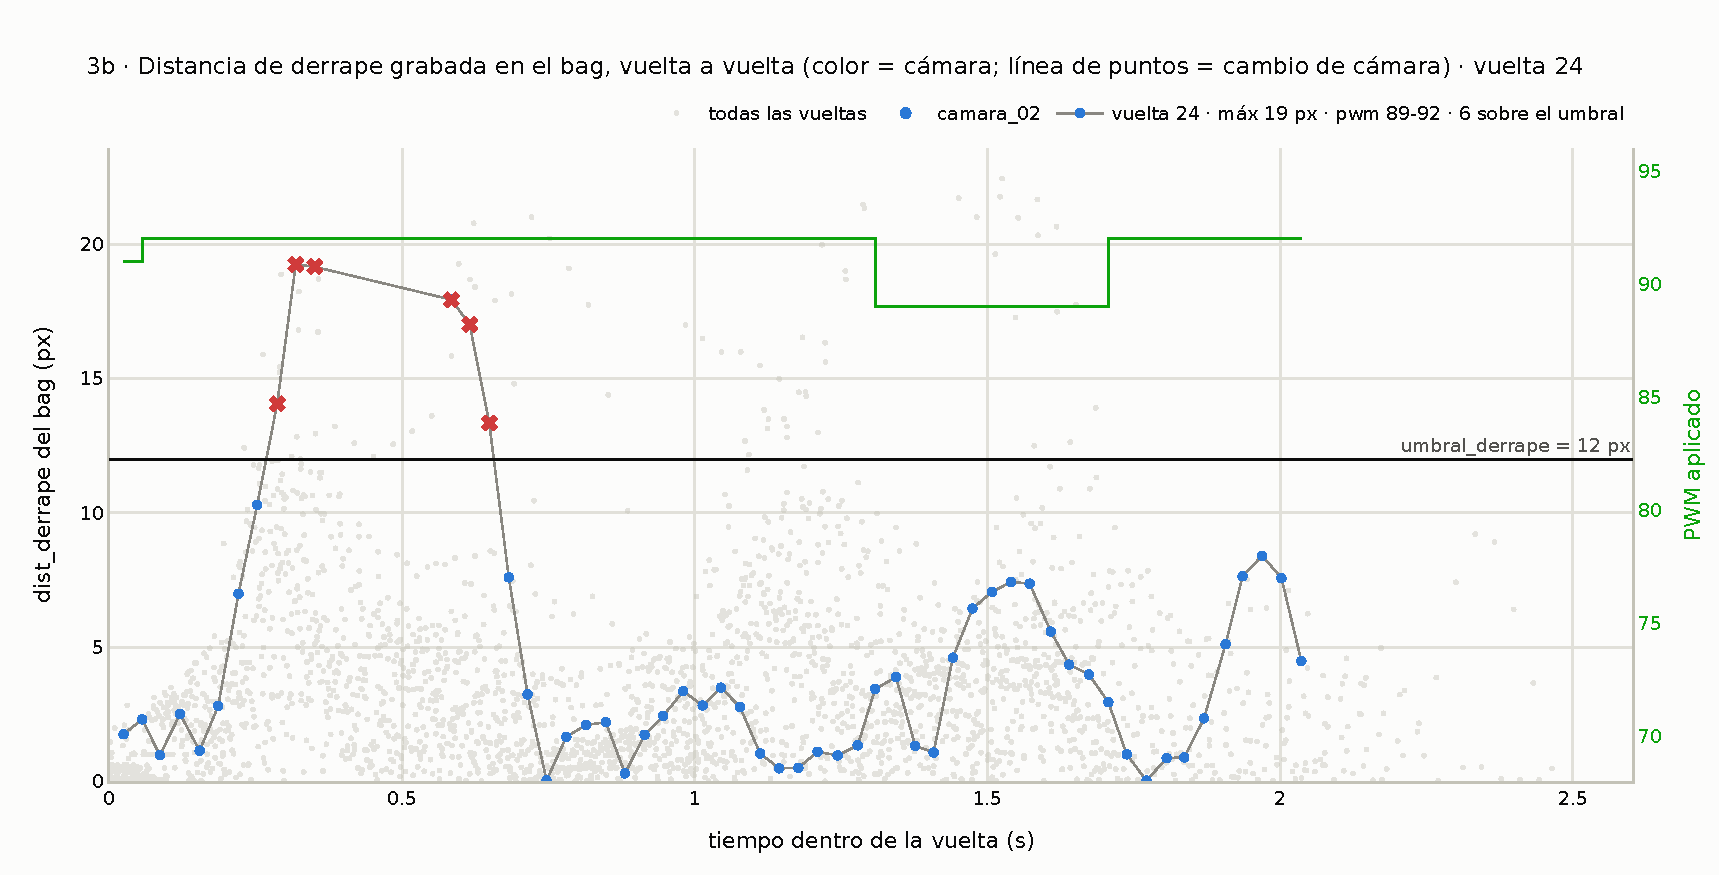
\includegraphics[trim={0 0 0 43pt},clip,width=\linewidth]{imaxes/PRUEBAS/ALGO_VARIOS_PARAMETROS/derrape_explosivo.pdf}
    \caption{Umbral de derrape 12~px, vuelta 24}
    \label{fig:derrape-explosivo}
  \end{subfigure}
  \caption{Saltos en la distancia de derrape del coche azul. Las cruces rojas son las muestras que superan el umbral y el fondo gris, el resto de vueltas de la ejecución}
  \label{fig:derrape-vuelta}
\end{figure}

Las métricas de las tres ejecuciones se recogen en la tabla~\ref{tab:parametros-azul} y permiten precisar en qué consiste la mejora. Las medianas de las dos configuraciones con PWM 70--94 son casi iguales, 1,733~s frente a 1,755~s, y las mejores vueltas resultan indistinguibles, 1,663~s frente a 1,661~s, de modo que bajar el umbral no hace al coche más rápido en su vuelta buena, sino que le quita las vueltas malas. Eso se refleja en la media, que cae de 1,872~s a 1,759~s, y en la peor vuelta, que pasa de 2,839~s a 2,418~s, y sobre todo en la desviación típica, que se reduce a menos de la mitad, de 0,228~s a 0,094~s. Sobre las 50 vueltas la diferencia acumulada es de 5,66~segundos, así que en una carrera entre ambas configuraciones ganaría la más conservadora, que mantiene el ritmo, frente a la que pierde varias décimas cada vez que tarda en detectar un derrape.

\begin{table}[tbp]
  \centering
  \estilotabla[3]
  \caption{Métricas de tiempo por vuelta del coche azul en el circuito en óvalo para las tres configuraciones probadas.}
  \label{tab:parametros-azul}
  \begin{tabular}{lrrrrr}
    \toprule
    \rowcolor{ArqAzulClaro}
    Ejecución & Contrarreloj & Mejor & Mediana & Media & $\sigma$ \\
              \rowcolor{ArqAzulClaro} & (s) & (s) & (s) & (s) & (s) \\
    \midrule
    ALGO 012 (70--90, 12~px) & 96,41 & 1,731 & 1,788 & 1,928 & 0,291 \\
    ALGO 013 (70--94, 12~px) & 93,59 & 1,661 & 1,755 & 1,872 & 0,228 \\
    ALGO 014 (70--94, 9~px)  & 87,93 & 1,663 & 1,733 & 1,759 & 0,094 \\
    \bottomrule
  \end{tabular}
\end{table}

ALGO 012 mantiene el umbral permisivo de 12~px pero rebaja el techo de PWM de 94 a 90, y es la peor de las tres en todas las métricas, con 96,41~s de tiempo acumulado y una desviación típica de 0,291~s. Bajar el techo de velocidad penaliza el ritmo sin resolver los derrapes, porque el problema no era ir demasiado deprisa sino reaccionar demasiado tarde, y por eso la mejora viene de afinar el umbral y no de conducir más despacio.

\section{Prueba del algoritmo frente a pilotos humanos}
\label{sec:prueba-algo-vs-personas}

Existe una prueba equivalente en el trabajo de Adrián~\cite{tfgadrian}, pero abarca muy pocas vueltas y no es lo suficientemente preciso en el análisis.

Para las ejecuciones automáticas se reutilizaron los datos de las pruebas de las secciones~\ref{sec:prueba-comparativa-coches} y~\ref{sec:prueba-algo-parametros}. Para las manuales se levantó un nodo de cámara y un nodo controlador en la misma máquina, con el controlador en modo manual, se detalla cómo funciona en la sección~\ref{subsec:modos-operacion}. Cada piloto completó también 50 vueltas y después se apagó el sistema, con lo que todas las ejecuciones son directamente comparables.

La prueba se repitió en dos circuitos. El primero es el óvalo ya empleado en las pruebas anteriores, cubierto por una sola cámara. El segundo es el circuito en ocho, que necesita dos cámaras, una de ellas en la misma máquina que el nodo controlador y el puente Arduino y la otra en un segundo equipo que envía sus detecciones por red, de modo que este escenario añade la conmutación entre cámaras y la latencia de la red.

Las tablas~\ref{tab:vs-personas-azul} y~\ref{tab:vs-personas-rojo} recogen los resultados sobre el óvalo y en los dos coches se repite el mismo patrón. Los pilotos humanos firman las mejores vueltas absolutas, 1,276~s y 1,291~s en el coche rojo frente a los 1,315~s de la mejor ejecución automática, pero ninguno de los dos gana la contrarreloj. La explicación está en la desviación típica, de 0,787~s y 1,151~s en el caso de los pilotos frente a valores en torno a 0,22~s en las ejecuciones automáticas. El piloto encuentra el límite del coche en una vuelta concreta y no consigue repetirlo, y cada intento fallido le cuesta más de lo que le había ganado el intento bueno.

\begin{table}[tbp]
  \centering
  \estilotabla[3]
  \caption{Coche azul en el circuito en óvalo, algoritmo vs pilotos humanos.}
  \label{tab:vs-personas-azul}
  \begin{tabular}{lrrrrr}
    \toprule
    \rowcolor{ArqAzulClaro}
    Ejecución & Contrarreloj & Mejor & Mediana & Media & $\sigma$ \\
              \rowcolor{ArqAzulClaro} & (s) & (s) & (s) & (s) & (s) \\
    \midrule
    ALGO 014 (70--94, 9~px)  & 87,93 & 1,663 & 1,733 & 1,759 & 0,094 \\
    ALGO 013 (70--94, 12~px) & 93,59 & 1,661 & 1,755 & 1,872 & 0,228 \\
    Manual (piloto 1)        & 94,30 & 1,659 & 1,833 & 1,886 & 0,197 \\
    ALGO 012 (70--90, 12~px) & 96,41 & 1,731 & 1,788 & 1,928 & 0,291 \\
    Manual (piloto 2)        & 107,54 & 1,674 & 1,911 & 2,151 & 0,646 \\
    \bottomrule
  \end{tabular}
\end{table}

\begin{table}[tbp]
  \centering
  \estilotabla[3]
  \caption{Coche rojo en el circuito en óvalo, algoritmo vs pilotos humanos.}
  \label{tab:vs-personas-rojo}
  \begin{tabular}{lrrrrr}
    \toprule
    \rowcolor{ArqAzulClaro}
    Ejecución & Contrarreloj & Mejor & Mediana & Media & $\sigma$ \\
              \rowcolor{ArqAzulClaro} & (s) & (s) & (s) & (s) & (s) \\
    \midrule
    ALGO 013 (70--94, 12~px) & 75,44 & 1,315 & 1,377 & 1,509 & 0,232 \\
    ALGO 014 (70--94, 9~px)  & 75,67 & 1,329 & 1,399 & 1,513 & 0,214 \\
    ALGO 012 (70--90, 12~px) & 80,82 & 1,436 & 1,510 & 1,616 & 0,220 \\
    Manual (piloto 1)        & 82,36 & 1,291 & 1,421 & 1,647 & 0,787 \\
    Manual (piloto 2)        & 93,86 & 1,276 & 1,587 & 1,877 & 1,151 \\
    \bottomrule
  \end{tabular}
\end{table}

La diferencia entre los dos coches también reaparece aquí, como ya habíamos intuido en las pruebas anteriores. En el rojo la mejor ejecución automática le saca casi 7~segundos al mejor piloto, mientras que en el azul el margen se estrecha hasta los 0,7~segundos que separan a ALGO 013 del piloto 1, porque el coche es tan sensible que encontrar el punto de funcionamiento correcto resulta difícil para las dos partes. De hecho ALGO 012, con los parámetros mal ajustados, queda por debajo del piloto 1 en una de las ejecuciones.

% ---------------------------------------------------------------------
%  Circuito en ocho
% ---------------------------------------------------------------------

Los resultados sobre el circuito en ocho se recogen en las tablas~\ref{tab:vs-personas-ocho-azul} y~\ref{tab:vs-personas-ocho-rojo}. Este trazado es bastante más exigente que el óvalo, porque ya no basta con sostener una potencia constante: hay que frenar y volver a acelerar en los sitios adecuados.

\begin{table}[tbp]
  \centering
  \estilotabla[3]
  \caption{Coche azul en el circuito en ocho, algoritmo vs pilotos humanos.}
  \label{tab:vs-personas-ocho-azul}
  \begin{tabular}{lrrrrr}
    \toprule
    \rowcolor{ArqAzulClaro}
    Ejecución & Contrarreloj & Mejor & Mediana & Media & $\sigma$ \\
              \rowcolor{ArqAzulClaro} & (s) & (s) & (s) & (s) & (s) \\
    \midrule
    ALGO 002 (60--75, 9~px)  & 202,89 & 3,588 & 3,804 & 4,058 & 0,626 \\
    ALGO 004 (63--85, 8~px)  & 205,00 & 3,549 & 4,011 & 4,100 & 0,563 \\
    ALGO 001 (60--75, 10~px) & 210,22 & 3,576 & 3,885 & 4,204 & 0,733 \\
    ALGO 003 (60--85, 9~px)  & 243,92 & 3,697 & 4,200 & 4,878 & 2,094 \\
    Manual (piloto 2)        & 276,72 & 3,972 & 4,893 & 5,534 & 1,876 \\
    Manual (piloto 3)        & 427,23 & 4,615 & 6,589 & 8,545 & 4,997 \\
    \bottomrule
  \end{tabular}
\end{table}

En el coche azul la distancia entre el algoritmo y los pilotos se dispara respecto al óvalo. ALGO 002 completa las 50 vueltas en 202,89~s y el mejor de los dos pilotos necesita 276,72~s, un 36\,\% más, mientras que el segundo se va hasta los 427,23~s, más del doble. Aquí ya no se sostiene el consuelo del óvalo, porque la vuelta rápida también es del algoritmo, y ninguna de las cuatro configuraciones queda por detrás de un piloto, algo que allí sí llegó a pasar con ALGO 012. Entre esas cuatro se repite además el patrón de la sección~\ref{sec:prueba-algo-parametros}: ALGO 003 sube el techo de PWM a 85 sin tocar el umbral y es con diferencia la peor, con 243,92~s, mientras que ALGO 004 mantiene ese techo, baja el umbral a 8~px y vuelve a los 205,00~s, de modo que el techo se puede subir pero solo si el umbral se afina al mismo tiempo.

\begin{table}[tbp]
  \centering
  \estilotabla[3]
  \caption{Coche rojo en el circuito en ocho, algoritmo vs pilotos humanos.}
  \label{tab:vs-personas-ocho-rojo}
  \begin{tabular}{lrrrrr}
    \toprule
    \rowcolor{ArqAzulClaro}
    Ejecución & Contrarreloj & Mejor & Mediana & Media & $\sigma$ \\
              \rowcolor{ArqAzulClaro} & (s) & (s) & (s) & (s) & (s) \\
    \midrule
    ALGO 001 (60--75, 10~px)     & 138,23 & 2,603 & 2,713 & 2,765 & 0,152 \\
    Manual (piloto 1, intento 2) & 141,24 & 2,456 & 2,656 & 2,825 & 0,548 \\
    ALGO 003 (65--90, 10~px)     & 141,81 & 2,618 & 2,756 & 2,836 & 0,225 \\
    ALGO 002 (60--90, 10~px)     & 152,13 & 2,632 & 2,862 & 3,043 & 0,571 \\
    Manual (piloto 1, intento 4) & 154,87 & 2,387 & 2,567 & 3,097 & 1,307 \\
    Manual (piloto 1, intento 1) & 159,73 & 2,522 & 2,838 & 3,195 & 1,232 \\
    Manual (piloto 1, intento 3) & 162,10 & 2,424 & 2,689 & 3,242 & 1,659 \\
    Manual (piloto 2)            & 182,11 & 2,523 & 2,944 & 3,642 & 1,981 \\
    \bottomrule
  \end{tabular}
\end{table}

Con el coche rojo el resultado es mucho más ajustado, y es el que mejor ilustra la diferencia entre las dos formas de conducir. ALGO 001 gana la contrarreloj con 138,23~s y el mejor intento manual se queda a 3,01~s. El piloto 1 repitió la prueba cuatro veces y sus vueltas rápidas mejoraron en cada intento, de 2,522 a 2,387~s, hasta quedar por debajo de la mejor vuelta del algoritmo; en dos de ellos incluso su mediana, 2,656 y 2,567~s, baja de los 2,713~s de ALGO 001, así que su vuelta típica llega a ser más rápida que la del sistema. Lo que no mejora es el acumulado, porque sus cuatro contrarrelojes, 159,73, 141,24, 162,10 y 154,87~s, no dibujan ninguna tendencia.

La explicación está en las vueltas que la mediana no ve. Buscar la vuelta rápida saca el coche de la pista, y cada salida obliga a recogerlo, colocarlo y arrancar otra vez desde parado, de manera que un puñado de vueltas así borra todo lo ganado en las demás: la media ya se le da la vuelta al piloto, 2,825 y 3,097~s frente a los 2,765~s del algoritmo, y su desviación típica no baja de 0,548~s frente a los 0,152~s de ALGO 001. Si hubiese podido repetir su mejor vuelta las cincuenta veces habría cerrado en 119,35~s, casi 19~segundos por debajo del algoritmo, así que el margen existe; lo que no existe es la forma de sostenerlo. El piloto 2 es el mismo caso en su extremo, con una mejor vuelta perfectamente competitiva de 2,523~s y una contrarreloj de 182,11~s. Entre las configuraciones automáticas conviene señalar que ALGO 002 y ALGO 003 solo se diferencian en el suelo del rango, 60 frente a 65, y esos cinco puntos cuestan más de 10~segundos, 152,13 frente a 141,81~s: el suelo es el valor al que puede llegar el castigo, así que ajustar el rango no es solo cuestión de cuánto se deja correr al coche sino de cuánto se le permite frenar.

La comparación entre los dos coches vuelve a aparecer aquí y con más fuerza que en el óvalo. ALGO 001 se ejecutó con exactamente la misma configuración, con el rango de 60 a 75 y el umbral en 10~px, sobre los dos vehículos, y el resultado es de 210,22~s en el azul frente a 138,23~s en el rojo, casi 72~segundos y un 52\,\% más, cuando en el óvalo la misma comparación se quedaba en un 19\,\%. Un trazado más largo y con más curvas multiplica el efecto de la diferencia de adherencia descrita en la sección~\ref{sec:prueba-comparativa-coches}, y lo hace por igual para las dos partes, porque a los pilotos el coche azul también les cuesta mucho más que el rojo.

La conclusión de estas pruebas es que la ventaja del algoritmo no está en la velocidad punta sino en la capacidad de sostenerla. Un piloto humano iguala e incluso supera al sistema en una vuelta suelta, porque arriesga donde el algoritmo se limita a lo que ha aprendido, pero no consigue repetir ese riesgo cincuenta veces seguidas y en una carrera lo que cuenta es el acumulado. Cuanto más exigente es el trazado mayor es esa ventaja, porque la dificultad se le acumula al piloto vuelta tras vuelta mientras que al algoritmo solo le supone más zonas que ajustar. Esa regularidad es consecuencia directa de la política de castigo por zonas descrita en la sección~\ref{subsec:algoritmo-aprendizaje}, que sacrifica velocidad puntual en los tramos conflictivos a cambio de no perder vueltas enteras.

\section{Prueba de la política óptima}
\label{sec:prueba-politica-optima}

En esta prueba se enfrenta al algoritmo con una \emph{política óptima}, es decir, con un perfil ya fijado que asigna un valor de PWM a cada celda de la trayectoria base y que el controlador se limita a aplicar sin aprender nada, tal y como se describe en la sección~\ref{subsec:modos-operacion}. La motivación sale de las gráficas de tiempo de las pruebas anteriores, en las que a veces parece que el coche encuentra un buen ritmo y después vuelve a perderlo: si esa vuelta buena se pudiera congelar y repetir, los tiempos deberían mantenerse. Como el comportamiento del circuito cambia de un día para otro, según se vio en la sección~\ref{sec:prueba_pwm_incremental}, todo se hizo el mismo día sobre el mismo montaje, sin tocar la configuración y sin mover ni la pista ni la cámara, de modo que el contacto entre los carriles fuese el mismo en las cuatro ejecuciones. La primera es una ejecución de referencia con el algoritmo, con el coche azul, un rango de PWM de 65 a 88 y un umbral de derrape de 11~px, y de ella sale la política que después se repite tres veces.

La mejor vuelta de esa ejecución de referencia es la 17, con 1,681~s, y resulta ser también la vuelta en la que el coche derrapa, ya que su distancia máxima llega a 12,4~px con el umbral en 11. Tiene sentido, porque el algoritmo va subiendo la tensión poco a poco y esa es justo la primera vuelta en la que se pasa, de manera que el mejor tiempo se paga con la pérdida de adherencia que lo delata. Al cerrarse ese derrape el algoritmo castiga las celdas 44 a 57, y el perfil que queda inmediatamente después es el que se guardó como política: tres zonas sobre las 84 celdas de la trayectoria, las dos libres a PWM 83 y la de derrape a 79. El fichero completo está en el código~\ref{lst:politica-json}.

Los resultados se recogen en la tabla~\ref{tab:politica-tiempos} y a primera vista la política gana, porque completa las 50 vueltas entre 90,42 y 91,71~s frente a los 98,29~s del algoritmo, unos siete segundos menos. Pero ninguna de las tres repeticiones iguala la mejor vuelta del algoritmo, 1,681~s frente a 1,719, 1,760 y 1,766~s, y las medianas son prácticamente la misma en las cuatro, entre 1,797 y 1,814~s. La figura~\ref{fig:politica-tiempos} enseña de dónde sale entonces la diferencia: el algoritmo arranca en su tensión mínima y necesita catorce vueltas para ponerse al ritmo que la política lleva desde la primera, de modo que solo en las diez vueltas iniciales pierde 26,01~s frente a los 18,40~s de la política. Toda la ventaja está ahí.

\begin{table}[tbp]
  \centering
  \estilotabla[3]
  \caption{Métricas de las 50 vueltas de la ejecución de referencia con el algoritmo y de las tres repeticiones de la política congelada (coche azul, PWM 65--88, umbral de derrape 11~px).}
  \label{tab:politica-tiempos}
  \begin{tabular}{lrrrrr}
    \toprule
    \rowcolor{ArqAzulClaro}
    Ejecución & Contrarreloj & Mejor & Mediana & Media & $\sigma$ \\
              \rowcolor{ArqAzulClaro} & (s) & (s) & (s) & (s) & (s) \\
    \midrule
    Política 001 & 90,42 & 1,766 & 1,804 & 1,808 & 0,039 \\
    Política 002 & 91,64 & 1,719 & 1,797 & 1,833 & 0,137 \\
    Política 003 & 91,71 & 1,760 & 1,803 & 1,834 & 0,124 \\
    Algoritmo    & 98,29 & 1,681 & 1,814 & 1,966 & 0,393 \\
    \bottomrule
  \end{tabular}
\end{table}

\begin{figure}[tbp]
  \centering
  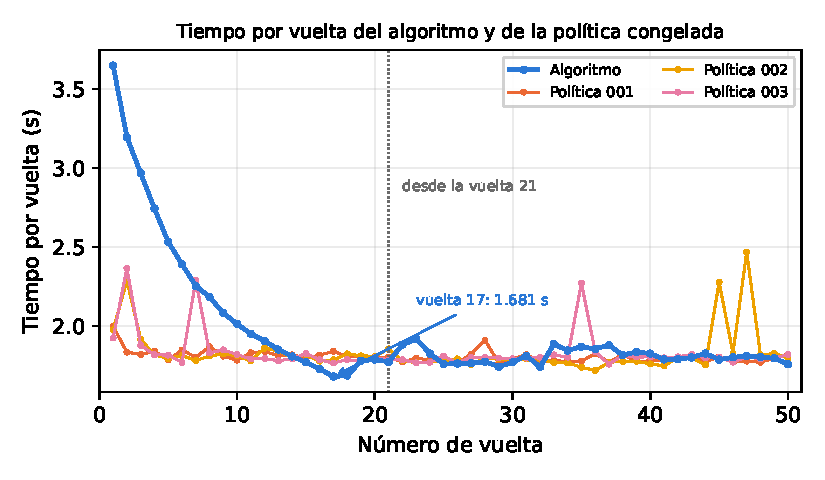
\includegraphics[trim={0 0 0 22},clip,width=\textwidth]{imaxes/PRUEBAS/POLITICA_OPTIMA/tiempos_politica.pdf}
  \caption{Tiempo por vuelta de las cuatro ejecuciones. Al algoritmo le cuesta catorce vueltas alcanzar el ritmo que la política ya lleva desde la primera}
  \label{fig:politica-tiempos}
\end{figure}

Si se descuentan esas vueltas de arranque la ventaja desaparece. La tabla~\ref{tab:politica-estable} recoge las mismas métricas a partir de la vuelta 21, que es cuando el tiempo del algoritmo deja de bajar, y las cuatro ejecuciones caben en 0,83~s sobre 30 vueltas, menos de tres centésimas por vuelta. Tampoco resulta la política más fiable, porque dos de las tres repeticiones derrapan bastante más que el algoritmo, con 82 y 96 muestras por encima del umbral frente a las 16 de la ejecución de referencia y con picos de 22,5 y 26,1~px que se traducen en vueltas sueltas de 2,468 y 2,366~s. Y eso que las tres se hicieron seguidas, en un cuarto de hora y sin tocar nada: el perfil congelado no puede echarse atrás cuando la pista cambia bajo él, mientras que el algoritmo baja la tensión de la zona en cuanto detecta el derrape.

\begin{table}[tbp]
  \centering
  \estilotabla[3]
  \caption{Las mismas métricas contando solo desde la vuelta 21, con el algoritmo ya estabilizado.}
  \label{tab:politica-estable}
  \begin{tabular}{lrrrrr}
    \toprule
    \rowcolor{ArqAzulClaro}
    Ejecución & Contrarreloj & Mejor & Mediana & Media & $\sigma$ \\
              \rowcolor{ArqAzulClaro} & (s) & (s) & (s) & (s) & (s) \\
    \midrule
    Política 001 & 53,85 & 1,766 & 1,783 & 1,795 & 0,028 \\
    Algoritmo    & 54,33 & 1,742 & 1,804 & 1,811 & 0,045 \\
    Política 003 & 54,43 & 1,760 & 1,803 & 1,814 & 0,087 \\
    Política 002 & 54,68 & 1,719 & 1,785 & 1,823 & 0,152 \\
    \bottomrule
  \end{tabular}
\end{table}

La conclusión es que aplicar una política fija sí permite empezar con buenos tiempos desde la primera vuelta, mientras que el algoritmo necesita unas cuantas iteraciones para llegar ahí, pero no da ninguna ventaja de ritmo y se paga con la adaptabilidad, ya que si el circuito cambia el algoritmo se adapta solo y la política hay que rehacerla. Guardarla tiene sentido para repetir carreras sobre un circuito que no se va a desmontar, y de hecho lo que esta prueba señala como mejorable del algoritmo no es su ritmo, que ya es el bueno, sino la rampa con la que arranca: partir de un perfil guardado o subir a escalones más grandes en las primeras vueltas le ahorraría los siete segundos que aquí pierde.

\section{Pruebas de red}
\label{sec:pruebas-red}

El objetivo de esta prueba es comprobar cuanto retardo añade la red al lazo de control y a partir de qué punto llega a notarse en la pista. Se hizo sobre el óvalo con una sola cámara, que es el trazado del que más datos se tienen y ser más sencillo de trabajar.

Todas las ejecuciones se hicieron con el coche azul, en el mismo carril, con la cámara sin mover y con la misma configuración: rango de PWM de 65 a 90 y umbral de derrape de 10~px. De cada escenario se hicieron tres repeticiones de 50 vueltas, 18 ejecuciones en total.

El retardo no se puede medir restando la marca de tiempo que la cámara pone en el mensaje menos el instante en que el controlador lo recibe, porque son dos relojes de dos máquinas distintas lo que puede ocasionar que haya desfase entre ellas. Por eso se añadió un nodo que manda a la cámara paquetes del tamaño de un mensaje de posición y cronometra lo que tardan en volver. Al ser un viaje de ida y vuelta las dos marcas las toma el mismo reloj y el desfase desaparece al restar, que es el motivo por el que el RFC~2681 define una métrica de ida y vuelta~\cite{rfc2681}. La cámara devuelve también lo que ha tardado ella en contestar, y ese tiempo se descuenta. De forma que el retardo podemos estimar como la mitad del tiempo que tardamos en hacer el viaje de ida y vuelta.

En los tres escenarios el nodo puente se ejecuta en la misma máquina que los controladores. Es una decisión de despliegue y no una limitación, esa máquina ya tiene que ser potente porque lleva un controlador por coche, y teniendo ese equipo lo razonable es enchufarle el Arduino y no añadir un salto de red entre decidir la tensión y aplicarla. La arquitectura permite separarlos, pero ese caso no se ha probado.

Los tres escenarios se diferencian solo en dónde corre el nodo cámara. En el primero, A1, los tres nodos están en el mismo ordenador y no hay red de por medio. En el segundo, A2, la cámara corre en la Raspberry Pi y conectado por cable al router al igual que el ordenador, y en el tercero, A3, la misma cámara conectaod por WIFI al router igual que el ordenador. Lo que viaja por ese enlace es la posición del coche, que es lo que el controlador necesita para aplicar el algoritmo.

La tabla~\ref{tab:red-rtt} recoge lo que mide el nodo de sondeo, el nodo que se creo y que envía mensajes para medir el tiempo de ida y vuelta. El peor escenario es el WiFi y aun así se queda en 7,27~ms de mediana, y en ninguno de los tres se perdió un solo paquete de los más de mil seiscientos que se enviaron. Que A1 no salga a cero, e incluso quede por encima del cable, puede ser algo no tan raro ya que esa máquina lleva encima además el nodo cámara, y pasar un mensaje entre dos procesos tampoco es gratis.

\begin{table}[tbp]
  \centering
  \estilotabla[3]
  \caption{Tiempo de ida y vuelta por escenario, con las tres repeticiones juntas.}
  \label{tab:red-rtt}
  \begin{tabular}{lrrrrr}
    \toprule
    \rowcolor{ArqAzulClaro}
    Escenario & Sondeos & Mediana & p95 & p99 & Máximo \\
              \rowcolor{ArqAzulClaro} & & (ms) & (ms) & (ms) & (ms) \\
    \midrule
    A1 (una máquina) & 1680 & 3,36 & 8,74 & 19,80 & 54,27 \\
    A2 (cable)       & 1720 & 2,42 & 10,00 & 12,54 & 16,92 \\
    A3 (WiFi)        & 1664 & 7,27 & 14,96 & 17,76 & 27,80 \\
    \bottomrule
  \end{tabular}
\end{table}

La figura~\ref{fig:red-cdf} enseña la medida completa. Las tres curvas suben de golpe y se plantan antes de los 20~ms. La del WiFi va desplazada unos milisegundos a la derecha de las otras dos, y esa es toda la diferencia entre las tres.

\begin{figure}[tbp]
  \centering
  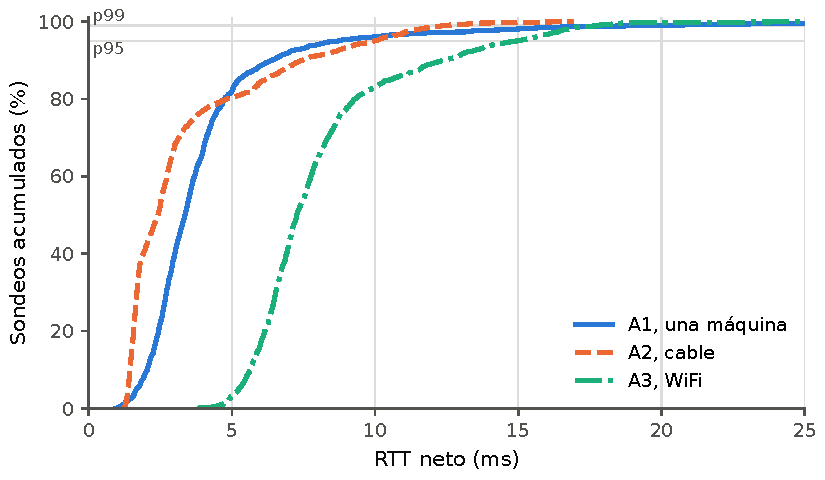
\includegraphics[width=\linewidth]{imaxes/PRUEBAS/RED/cdf_rtt.pdf}
  \caption{Distribución acumulada del tiempo de ida y vuelta. Fuera del eje queda un único sondeo de A1 de 54~ms.}
  \label{fig:red-cdf}
\end{figure}

Esos milisegundos hay que verlos al lado del resto del lazo, y eso es lo que hace la figura~\ref{fig:red-presupuesto}, que muestra como se reparte la latencia entre los tres pasos que van desde que se captura el fotograma hasta que el algoritmo devuelve el valor que hay que aplicar de tensión. El de la red es el más pequeño de los tres con diferencia, incluso por WiFi no llega a una quinta parte del total, que se queda en 22~ms. Y ese total cabe dentro de los 33~ms que pasan entre dos fotogramas.

\begin{figure}[tbp]
  \centering
  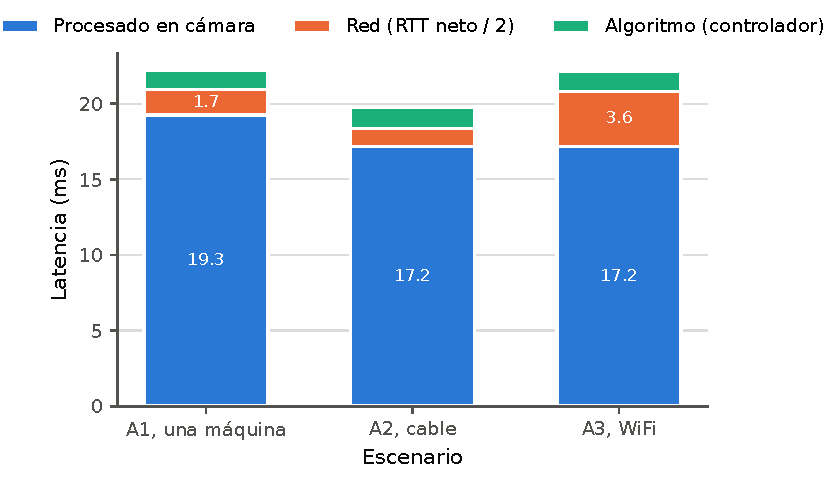
\includegraphics[width=\linewidth]{imaxes/PRUEBAS/RED/presupuesto_latencia.pdf}
  \caption{Reparto de la latencia del lazo entre sus tres pasos. El tramo de red es la mitad del tiempo de ida y vuelta.}
  \label{fig:red-presupuesto}
\end{figure}

Sobre la pista no se traduce en nada, y eso lo dice la tabla~\ref{tab:red-tiempos-a}. Los tres escenarios completan las 50 vueltas en un tiempo parecido y sus mejores vueltas se quedan en cuatro centésimas unas de otras, con el WiFi como el más rápido de los tres aun siendo el que más retardo tiene. Las tres repeticiones de A2 dieron 97,35, 100,63 y 104,51~s, así que dos ejecuciones del mismo escenario se separan más que los escenarios entre sí. Lo que se ve ahí es la variabilidad del coche y del circuito que ya describe la sección~\ref{sec:prueba_pwm_incremental}.

\begin{table}[tbp]
  \centering
  \estilotabla[3]
  \caption{Tiempos de las 50 vueltas por escenario.}
  \label{tab:red-tiempos-a}
  \begin{tabular}{lrrrrr}
    \toprule
    \rowcolor{ArqAzulClaro}
    Escenario & Contrarreloj & Mejor & Mediana & Media & $\sigma$ \\
              \rowcolor{ArqAzulClaro} & (s) & (s) & (s) & (s) & (s) \\
    \midrule
    A3 (WiFi)        & 97,91 & 1,725 & 1,819 & 1,958 & 0,285 \\
    A2 (cable)       & 100,83 & 1,716 & 1,808 & 2,017 & 0,552 \\
    A1 (una máquina) & 102,45 & 1,740 & 1,843 & 2,049 & 0,405 \\
    \bottomrule
  \end{tabular}
\end{table}

Que la red no se note cuando es buena no dice hasta dónde aguanta el control cuando deja de serlo. Para verlo se repitió el escenario del WiFi añadiendo retardo a mano con \texttt{tc netem}~\cite{netem}, una herramienta del \emph{kernel} de Linux que retiene los paquetes el tiempo que se le indique. La regla se pone en la Raspberry Pi con \texttt{sudo tc qdisc add dev wlan1 root netem delay 25ms}, se pasa de un punto al siguiente cambiando \texttt{add} por \texttt{change}, y al terminar se quita con ese mismo comando y \texttt{del}. Se probaron 25, 50 y 100~ms, con tres repeticiones cada uno. No se subió más porque con más de 100~ms entre dos máquinas de la misma sala el problema ya no es el control.

Como la regla está en la salida de la Raspberry Pi, el retardo lo sufre el sentido cámara~$\rightarrow$~PC, que es justamente por donde viajan las posiciones, y por eso aparece una sola vez en el tiempo de ida y vuelta de la tabla~\ref{tab:red-tiempos-b}. Con 100~ms cada posición que recibe el controlador dice dónde estaba el coche hace una décima de segundo. Con el retardo puesto aparecen además mensajes perdidos, trece de unos cinco mil, pero concentrados en dos repeticiones sueltas y sin relación con el retardo aplicado.

\begin{table}[tbp]
  \centering
  \estilotabla[3]
  \caption{Retardo medido y tiempos de las 50 vueltas según el retardo inyectado. El punto de 0~ms es A3 sin tocar.}
  \label{tab:red-tiempos-b}
  \begin{tabular}{lrrrrrr}
    \toprule
    \rowcolor{ArqAzulClaro}
    Retardo & Ida y vuelta & Contrarreloj & Mejor & Mediana & Media & $\sigma$ \\
            \rowcolor{ArqAzulClaro}
    inyectado & (ms) & (s) & (s) & (s) & (s) & (s) \\
    \midrule
    0 ms   & 7,27 & 97,91 & 1,725 & 1,819 & 1,958 & 0,285 \\
    25 ms  & 33,21 & 100,98 & 1,750 & 1,870 & 2,020 & 0,322 \\
    50 ms  & 58,48 & 99,69 & 1,730 & 1,857 & 1,994 & 0,307 \\
    100 ms & 108,35 & 105,41 & 1,735 & 1,889 & 2,108 & 0,427 \\
    \bottomrule
  \end{tabular}
\end{table}

El coche completa sus 50 vueltas en los cuatro casos y la mejor vuelta no empeora en ninguno. Con 25 y 50~ms los tiempos no se distinguen del punto de partida. Con 100~ms sí aparece algo: las tres repeticiones de ese punto dieron 103,46, 105,16 y 107,62~s, todas por encima de cualquiera de las tres sin retardo, y la vuelta mediana sube de 1,819 a 1,889~s, es una subida pequeña pero relevante.

La conclusión es que la red no es lo que limita el control. Por cable o por WiFi añade unos pocos milisegundos, muy por debajo de lo que tarda la propia cámara en procesar el fotograma, y el sistema se comporta igual que con todo junto en una máquina. Hay que inyectar 100~ms, más de diez veces el peor retardo medido aquí, para que empiece a notarse algo, y ni siquiera entonces el coche pierde el control. Encaja con lo observado durante el resto del trabajo, ya que buena parte de las pruebas con dos cámaras se hicieron por WiFi sin que se notara ninguna diferencia.

\section{Pruebas en Circuitos Grandes}
\label{sec:pruebas-circuitos-grande}

Aparte de los resultados obtenidos en la realización de las pruebas de red, también hicimos dos circuitos un poco grandes para demostrar que la arquitectura es completamente funcional en circunstancias distribuidas con multiples camaras como también estaba pensado. Vamos a tener dos circuitos donde vamos a ver como se comporta el coche si somos capaces de controlador y ver lo qeu pasa. Para está prueab vamos va tener 2 rasberry pi 5 para controlar cada una como nodo camara y después en el ordenador vamos a tener un controlador y el nodo puente que permite controlar el arduino. 

\section{Prueba nodo visualización y multiples coches}
\label{sec:prueba-nodo-visualizacion-multiples-coches}

Esta es una pequeña prueba para ver como se comporta la arquitectura con varios coches y como funciona además el nodo de visualización que tenemos creado para controlarlo 

 \chapter{Conclusiones y trabajo futuro}
\label{cap:conclusiones}

\lettrine{E}{n} este último capítulo se presentan las conclusiones extraídas del trabajo realizado, valorando el grado de cumplimiento de los objetivos planteados en la introducción. Se comentan asimismo las principales limitaciones y dificultades encontradas durante el desarrollo, se reflexiona sobre las lecciones aprendidas y se proponen posibles líneas de trabajo futuro que den continuidad al proyecto.

% -----------------------------------------------------------------------------
\section{Conclusiones}
\label{sec:conclusiones}

El objetivo general del trabajo era evolucionar el sistema de control visual de coches tipo Scalextric hacia una arquitectura distribuida capaz de operar en tiempo real sobre circuitos de cualquier tamaño, y se ha alcanzado. El sistema monolítico heredado se ha descompuesto en tres tipos de nodos con responsabilidades delimitadas (captura y detección, control por carril y actuación sobre el hardware) que se comunican exclusivamente mediante mensajes a través de la red local, sin memoria compartida. Lo relevante de este diseño no es tanto que el sistema funcione repartido, sino que el reparto pasa a ser una decisión de despliegue y no una propiedad del código. Los mismos nodos, sin ningún cambio, cubren las tres configuraciones posibles: con todos ellos en una misma máquina se reproduce el escenario del trabajo de Mario López \cite{lopezcea}, con varios nodos cámara en un mismo equipo, junto al controlador y al puente, el de Adrián Rego \cite{rego} y repartiendo los nodos cámara entre distintas máquinas se obtiene el caso nuevo que este trabajo aporta. La arquitectura propuesta no sustituye a las anteriores, las contiene como casos particulares. De esa modularidad se deriva además un beneficio práctico: añadir una funcionalidad se reduce a escribir un nodo y publicar o suscribirse a los \emph{topics} correspondientes, sin tocar el resto, y así se incorporaron la telemetría, la herramienta de grabación, el panel de carrera en directo y el nodo de sondeo empleado en las pruebas de red.

La segunda conclusión, y probablemente la de mayor alcance, es que la red no es el factor que limita el control. Las pruebas de la sección~\ref{sec:pruebas-red} sitúan el peor escenario, el de WiFi, en 7,27~ms de mediana de ida y vuelta, sin una sola pérdida en más de mil seiscientos sondeos, y el tramo de red no llega a una quinta parte de los 22~ms que consume el lazo completo, que a su vez cabe holgadamente en los 33~ms que separan dos fotogramas. Sobre la pista la diferencia entre escenarios queda por debajo de la variabilidad que hay entre dos repeticiones del mismo escenario, y hubo que inyectar 100~ms de retardo artificial para apreciar algo en el cronómetro sin que el coche llegara siquiera a perder el control. Esto valida el supuesto sobre el que se apoya toda la propuesta.

La detección y el seguimiento se han evaluado con una y con varias cámaras, con solapamiento y sin él, y el algoritmo de control se ha adaptado para operar sobre ese entorno coordinando las instancias por cámara sobre una trayectoria base común. La prueba frente a pilotos humanos de la sección~\ref{sec:prueba-algo-vs-personas} permite valorar el resultado el sistema gana la contrarreloj en todos los casos.

Conviene señalar, por último, un resultado que no figuraba entre los objetivos iniciales pero que ha acabado siendo determinante: la telemetría de todas las etapas del procesamiento junto con las herramientas de grabación y análisis en diferido de la sección~\ref{sec:sistema-visualizacion}. En una arquitectura de nodos independientes esta instrumentación es prácticamente gratuita, porque basta con suscribirse a lo que ya circula por la red, y sin ella no habría sido posible descomponer la latencia del lazo, comparar ejecuciones separadas por semanas ni detectar los problemas de hardware que se describen a continuación y que en los trabajos anteriores no aparecen reportados. El trabajo entrega por tanto una arquitectura estable sobre la que seguir construyendo, un análisis que permite saber dónde está el margen de mejora y unas herramientas de análisis que hasta ahora no existían.

% -----------------------------------------------------------------------------
\section{Limitaciones y dificultades encontradas}
\label{sec:limitaciones}

La planificación inicial asumió que la detección del coche estaba resuelta en los trabajos previos, que el algoritmo de control estaba correctamente implementado y que el hardware funcionaba de forma fiable. Las tres suposiciones resultaron ser solo parcialmente ciertas y condicionaron el desarrollo. La primera consecuencia fue de coste: aunque las ideas de detección por color y de seguimiento mediante región de interés estaban documentadas, la implementación no era reutilizable, al tratarse de código fuertemente cohesionado con la aplicación de escritorio y con su estado compartido en memoria, y hubo que reimplementar desde cero prácticamente toda la parte de visión. La segunda fue de diseño: al dar por buena la calidad del control heredado, el esfuerzo se orientó a distribuirlo antes que a revisarlo, y sus problemas solo se hicieron visibles cuando ya existían las herramientas para medirlos, con poco margen para replantear el enfoque. Tercero el hardware tenía problemas en el diseño que no sé detectaron hasta casi la fase final del proyecto mientras se estaban terminando las pruebas.

El conjunto pista+coche+arduino ha resultado ser mucho menos determinista de lo previsto y es la fuente principal de las limitaciones del sistema. Con la misma configuración, el coche rojo completa las 50 vueltas 18 segundos antes que el azul, más de un 19~\% del tiempo total en el óvalo y hasta un 52~\% en el circuito en ocho, por diferencias en el coche ajenas al control. Y el mismo coche sobre el mismo circuito dio 1,774~s por vuelta un día y 3,095~s otro con idéntico valor de PWM, hasta el punto de necesitar 110 para acercarse al tiempo que semanas antes se conseguía con 74. A esa variabilidad contribuyen el montaje de la pista con piezas de varios modelos, el estado de las escobillas de contacto, la limpieza de raíles y neumáticos y el desgaste acumulado de un material que lleva varios cursos en uso. La actuación tampoco ayuda: el rango de PWM realmente utilizable es estrecho, su relación con el incremento no es lineal.

Al algoritmo se le detectaron también limitaciones propias. La única señal que dispara el castigo de una zona es la separación de la etiqueta trasera respecto a la trayectoria base, un criterio binario que penaliza igual un derrape que empeora el tiempo por vuelta y otro que no lo hace, y que además resulta extremadamente sensible al umbral escogido, pasar de 12 a 9~px reduce la contrarreloj de 93,59 a 87,93~s y la desviación típica a menos de la mitad, como se ve en la sección~\ref{sec:prueba-algo-parametros}. Hay además derrapes que ese criterio no puede ver, porque el coche, tras ganar inercia progresivamente, sale disparado en un intervalo que con un muestreo de 33~ms no permite, por lo que por muy bien afinado que esté no hay información suficiente para reaccionar. Tampoco existe adaptación del rango, cuando el circuito responde peor de lo habitual el algoritmo agota su techo sin alcanzar la velocidad esperada y no dispone de mecanismo para elevarlo, de forma que la única salida es relanzarlo o retocar los parámetros en caliente. Y todo el sistema (la localización sobre el circuito, la partición en zonas, la máscara de búsqueda y la propia detección de derrapes) se apoya en la trayectoria base registrada en la calibración y se expresa en píxeles, así que cualquier cambio en el trazado, en la posición de la cámara o en la resolución obliga a recalibrar.

% -----------------------------------------------------------------------------
\section{Lecciones aprendidas}
\label{sec:lecciones}

Buena parte de las dificultades descritas vienen de haber dado por resueltos unos cimientos que solo lo estaban en parte, y validarlos antes de comprometer la planificación habría permitido detectar los problemas del hardware y del algoritmo mucho antes. De ahí se deriva la segunda, la instrumentación no es un accesorio que se añade al final, sino la condición para poder afirmar algo sobre el sistema; hasta que no existieron la telemetría y la herramienta de análisis, los problemas del circuito eran una sospecha.

Trabajar sobre un sistema físico ha exigido además ser mucho más riguroso con el diseño de los experimentos. Cuando el resultado depende del código pero también del coche, del montaje de la pista y de la alimentación, una ejecución aislada no permite concluir nada. Hay que decidir de antemano qué variable se quiere medir, fijar todas las demás y repetir cada escenario lo suficiente como para distinguir un efecto real de la dispersión propia del montaje. Las pruebas del capítulo~7 se plantearon así, y es lo que permitió separar las limitaciones del algoritmo de las del hardware.

% -----------------------------------------------------------------------------
\section{Trabajo futuro}
\label{sec:trabajofuturo}

El desarrollo ha dejado abiertas varias líneas de continuidad:

\begin{itemize}
\item \textbf{Revisar el criterio de derrape.} Sustituir el umbral único por un criterio que correlacione la separación de la trayectoria con el tiempo realmente perdido en esa zona, de modo que solo se penalicen los derrapes que empeoran la vuelta.

\item \textbf{Búsqueda automática de parámetros.} El sistema ya carga y ejecuta políticas que asignan un PWM a cada celda, lo que permite buscarlas mediante programación genética, optimización bayesiana o aprendizaje por refuerzo, usando el tiempo por vuelta y las salidas de pista como función objetivo. La herramienta de grabación aporta ya los datos para entrenar y evaluar fuera de línea.

\item \textbf{Rango de PWM adaptativo.} Permitir que el algoritmo eleve su propio techo cuando detecte que el circuito no responde como se espera, evitando el reajuste manual de un día para otro.

\item \textbf{Reducir la dependencia de la trayectoria base.} Explorar calibraciones que no exijan una vuelta de registro completa o que se actualicen de forma incremental.

\item \textbf{Renovar el material y fijar un protocolo de puesta a punto.} La pista, los coches y las cámaras acumulan un desgaste que condiciona los resultados; una mayor frecuencia de captura atacaría además el problema de los derrapes no observables.

\item \textbf{Nodos dedicados a la observación.} Sacar la publicación de imágenes de depuración del nodo cámara para descargar el camino crítico del lazo de control y simplificar su integración con el nodo de visualización.

\item \textbf{Automatizar el despliegue.} Con acceso SSH a todas las máquinas, una herramienta como Ansible permitiría levantar el sistema completo desde un único equipo, en lugar de ir máquina por máquina, y una interfaz de configuración facilitaría la edición de parámetros y la elección de qué nodos arrancar.

\item \textbf{Monitorizar el estado del sistema.} Vigilar qué nodos están vivos y a qué cadencia publican, y sincronizar los relojes mediante NTP o PTP para poder medir latencias en un solo sentido.
\end{itemize}


 %%%%%%%%%%%%%%%%%%%%%%%%%%%%%%%%%%%%%%%%
 % Apéndices, glosarios e bibliografía  %
 %%%%%%%%%%%%%%%%%%%%%%%%%%%%%%%%%%%%%%%%

 \appendix
 \appendixpage
 \chapter{Ejecución del sistema}
\label{chap:execucion}

\lettrine{E}{n} este anexo se describen los pasos necesarios para desplegar y ejecutar el
sistema completo: el software requerido en cada máquina, la preparación del hardware y los
comandos de lanzamiento de cada uno de los roles (nodos cámara y nodo cerebro).

\section{Software requerido}
\label{sec:software-requerido}

% TODO: Enumerar: sistema Linux con Docker y docker-compose instalados en cada máquina
% de la red (no es necesario instalar ROS2 en el anfitrión: va dentro de la imagen),
% git para clonar el repositorio, y acceso a la misma red local en todas las máquinas.

\section{Preparación del hardware}
\label{sec:preparacion-hardware}

% TODO: Describir:
%  - Montaje del circuito y colocación de las cámaras cubriendo todo el trazado.
%  - Pegatinas de colores en los coches (delantera y trasera) y marca de línea de
%    meta de color naranja visible por una de las cámaras.
%  - Carga del firmware en el Arduino y conexión del L293D a los carriles.
%  - Conexión del Arduino por USB a la máquina cerebro (/dev/ttyACM0).

\section{Instrucciones de ejecución}
\label{sec:instrucions-execucion}

% TODO: Documentar los comandos reales:
%
% En cada máquina con cámara (ajustando NODE_ID y CAMERA_DEV):
%
%   cd python
%   NODE_ID=camara_01 CAMERA_DEV=0 docker compose -f docker-compose-camera.yml up
%
% En la máquina cerebro (conectada al Arduino):
%
%   cd python
%   docker compose -f docker-compose-brain.yml up
%
% Explicar el flujo tras el arranque: los carriles se alimentan a la velocidad de
% calibración, el coche da la vuelta de calibración, al cruzar la meta el sistema pasa
% automáticamente a modo carrera. Para recalibrar: publicar True en /modo_calibracion
% o borrar los ficheros de caché (cache_trayectoria_*.json).

\section{Configuración}
\label{sec:configuracion-anexo}

% TODO: Referenciar python/src/image_processor_pkg/config/params.yaml y comentar los
% parámetros que el usuario puede querer ajustar: lista de coches, colores de las
% pegatinas y de la meta, resolución de cámara (camera.mode), velocidades mínima y
% máxima del controlador, velocidad de calibración y puerto del Arduino.

 \chapter{Detalle del nodo de captura y detección}
\label{chap:anexo-captura}

\lettrine{E}{n} este anexo se detalla el procesamiento de imagen del nodo de captura, resumido en la sección~\ref{sec:nodo-camara}. El nodo se divide en dos componentes: el nodo de ROS~2, que gestiona la comunicación y los modos de funcionamiento, y un objeto que encapsula las operaciones de visión artificial con las que se obtiene el centroide de cada pegatina. Logrando desacoplar el procesamiento de imagen de la comunicación.

\section{Detección de las pegatinas por color}
\label{subsec:deteccion-etiquetas}

La detección hereda el procedimiento del trabajo de Mario López~\cite{tfgmario}. El fotograma se convierte al espacio HSV, que resiste mejor las variaciones de iluminación, y se genera una máscara binaria por pegatina con los píxeles que caen dentro del rango de su color. Están predefinidos para cada uno de los siete colores admitidos. Sobre cada máscara se encadenan una apertura morfológica, que elimina los píxeles aislados, y un cierre morfológico, que rellena los huecos de las regiones válidas.

Se extraen entonces los contornos externos y se toma el de mayor área, descartándolo si no supera un área mínima configurable. De este proceso se obtiene el rectángulo delimitador y el centroide de la pegatina, el significado para cada pegatina se describió en la sección~\ref{sec:arquitectura}. La figura~\ref{fig:deteccion-color} recorre estas etapas sobre un fotograma real.

\begin{figure}[tbp]
    \centering
    \begin{subfigure}[b]{0.48\textwidth}
        \centering
        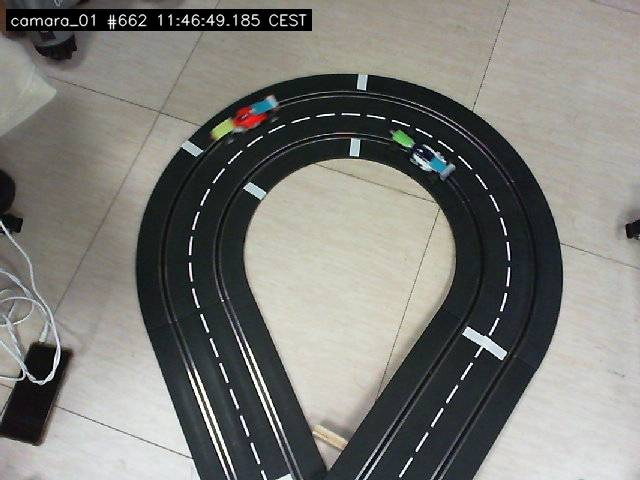
\includegraphics[width=\textwidth]{imaxes/IMPLEMENTACION/det_color_a_original.png}
        \caption{Fotograma capturado por la cámara}
        \label{fig:deteccion-color-a}
    \end{subfigure}
    \hfill
    \begin{subfigure}[b]{0.48\textwidth}
        \centering
        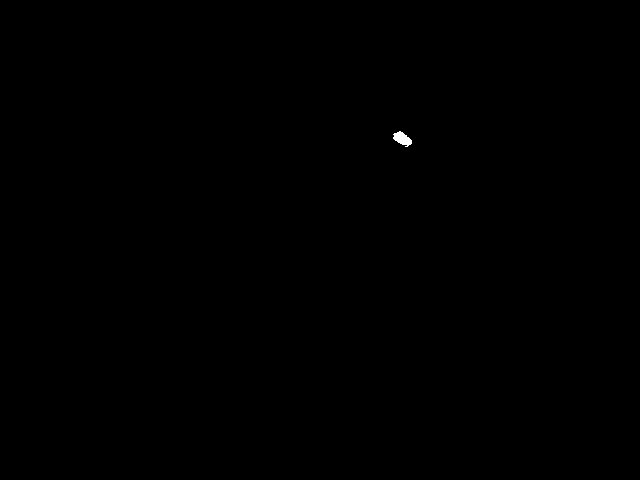
\includegraphics[width=\textwidth]{imaxes/IMPLEMENTACION/det_color_b_mascara.png}
        \caption{Máscara del color de la pegatina verde delantera del coche azul}
        \label{fig:deteccion-color-b}
    \end{subfigure}

    \vspace{0.7em}
    \begin{subfigure}[b]{0.34\textwidth}
        \centering
        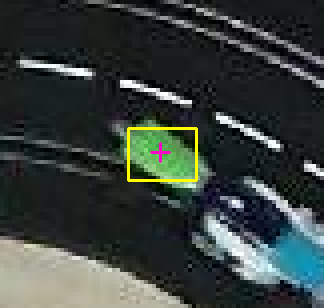
\includegraphics[width=\textwidth]{imaxes/IMPLEMENTACION/det_color_c_resultado.png}
        \caption{Rectángulo y centroide detectados después de realizar las operaciones pertinentes}
        \label{fig:deteccion-color-c}
    \end{subfigure}
    \caption{Ejemplo del proceso de detección que realiza el nodo camara para detectar una de las pegatinas del coche}
    \label{fig:deteccion-color}
\end{figure}

\section{Diferencias entre calibración y carrera}
\label{subsec:modos-funcionamiento}

El nodo implementa los dos modos descritos en la sección~\ref{sec:arquitectura}, y la diferencia entre ambos está en la región del fotograma sobre la que busca.

En calibración, cada detección de la pegatina delantera se añade a la lista que reconstruye la trayectoria del coche. Basta con la delantera, que es la que da una trayectoria limpia~\cite{tfgadrian}. Esto es porque la trasera puede quedar oculta a ratos y la ruta base debe registrarse sin interrupciones. Al mantener una trayectoria por coche, la cámara puede filtrar por carril en carrera y dos coches pueden compartir el color de la pegatina trasera. Durante todo este proceso se busca sobre el fotograma completo como el que se puede ver \ref{fig:deteccion-color-a}, es por ello que las pegatinas delanteras sí que tienen que ser de diferente color.

La calibración termina por coche, no para todo el sistema. El nodo se suscribe al \emph{topic} de calibración de cada coche configurado y, al recibir el aviso de que uno ha completado su vuelta, genera su máscara con los puntos acumulados. Desde ese momento la búsqueda de ese coche queda restringida a una franja alrededor del recorrido conocido, como recoge la figura~\ref{fig:mascara-trayectoria}.

\begin{figure}[tbp]
    \centering
    \begin{subfigure}[b]{0.32\textwidth}
        \centering
        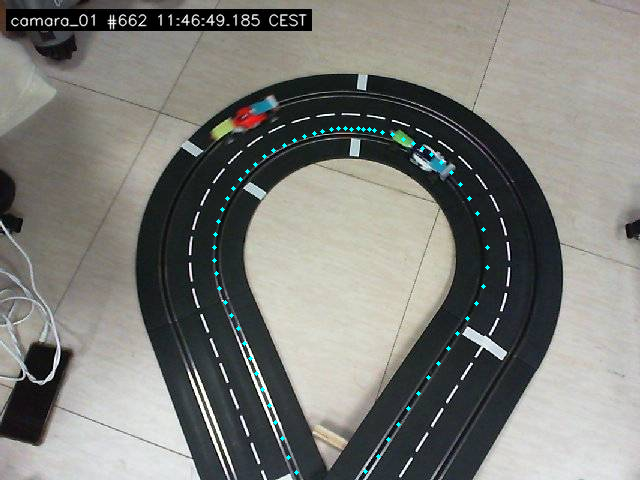
\includegraphics[width=\textwidth]{imaxes/IMPLEMENTACION/mascara_a_puntos.png}
        \caption{Posiciones acumuladas durante la vuelta de calibración}
        \label{fig:mascara-trayectoria-a}
    \end{subfigure}
    \hfill
    \begin{subfigure}[b]{0.32\textwidth}
        \centering
        
\includegraphics[width=\textwidth]{imaxes/IMPLEMENTACION/mascara_b_mascara.png}
        \caption{Máscara generada a partir de la posición que sigue el coche}
        \label{fig:mascara-trayectoria-b}
    \end{subfigure}
    \hfill
    \begin{subfigure}[b]{0.32\textwidth}
        \centering
        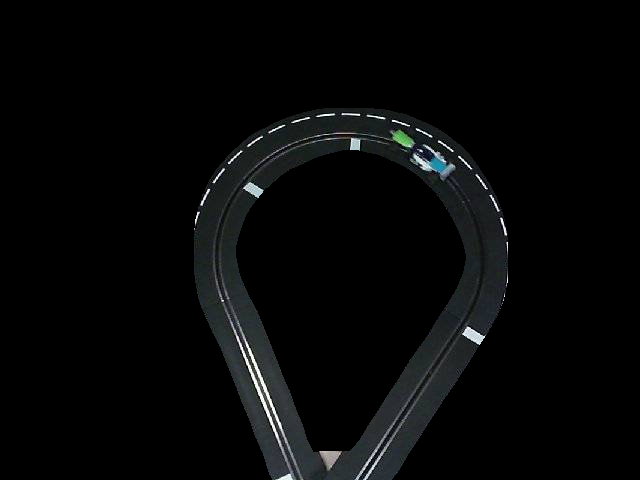
\includegraphics[width=\textwidth]{imaxes/IMPLEMENTACION/mascara_c_filtrado.png}
        \caption{Fotograma filtrado después de aplicar la mascara generada durante la calibración}
        \label{fig:mascara-trayectoria-c}
    \end{subfigure}
    \caption{Ejemplo de proceso de generación de la máscara de trayectoria para un coche. Deja fuera el carril contrario, con lo que el coche que circula por él deja de ser un falso positivo posible.}
    \label{fig:mascara-trayectoria}
\end{figure}

\section{Seguimiento mediante región de interés}
\label{subsec:seguimiento-roi}

En carrera la búsqueda se restringe a una región de interés de $150 \times 150$ píxeles centrada en la posición predicha para el coche. La predicción es la extrapolación lineal que introdujo Mario López~\cite{tfgmario}. Conocidas las dos últimas posiciones, el centro de la región es la actual más el vector de movimiento del último fotograma.

Sobre ella se aplica además la máscara de trayectoria, de modo que solo sobreviven los píxeles que pertenecen a la vez a la región y a las proximidades del carril; la intersección de ambos filtros procede también de los trabajos previos~\cite{tfgmario,tfgadrian}. La detección de las pegatinas (\ref{subsec:deteccion-etiquetas}) se realiza sobre esa imagen reducida, se puede ver un ejemplo en \ref{fig:roi-filtrado}. El problema que presenta hacerlo de esta manera es que sus coordenadas son relativas a la región y hay que trasladarlas al sistema de referencia de la cámara antes de publicarlas.

\begin{figure}[tbp]
    \centering
    \begin{subfigure}[b]{0.55\textwidth}
        \centering
        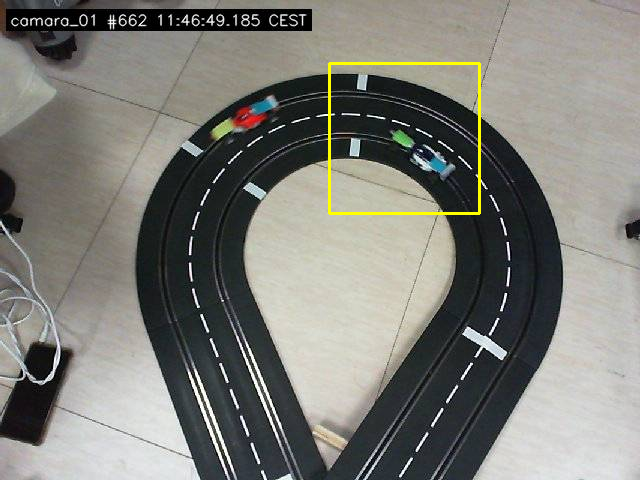
\includegraphics[width=\textwidth]{imaxes/IMPLEMENTACION/roi_a_recuadro.png}
        \caption{Región de interés marcada sobre todo el fotograma}
        \label{fig:roi-filtrado-a}
    \end{subfigure}
    \hfill
    \begin{subfigure}[b]{0.38\textwidth}
        \centering
        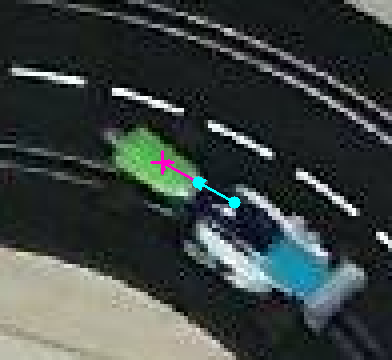
\includegraphics[width=\textwidth]{imaxes/IMPLEMENTACION/roi_b_extrapolacion.png}
        \caption{Extrapolación de la posición}
        \label{fig:roi-filtrado-b}
    \end{subfigure}

    \vspace{0.7em}
    \begin{subfigure}[b]{0.32\textwidth}
        \centering
        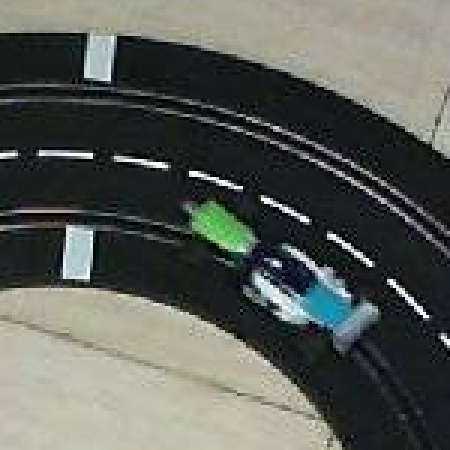
\includegraphics[width=\textwidth]{imaxes/IMPLEMENTACION/roi_c_recorte.png}
        \caption{Recorte de la región}
        \label{fig:roi-filtrado-c}
    \end{subfigure}
    \hspace{0.04\textwidth}
    \begin{subfigure}[b]{0.32\textwidth}
        \centering
        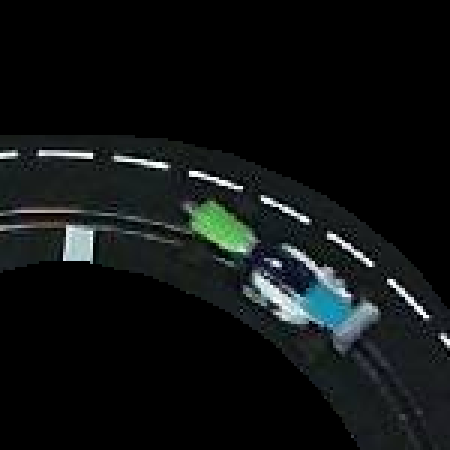
\includegraphics[width=\textwidth]{imaxes/IMPLEMENTACION/roi_d_filtrado.png}
        \caption{Región tras la intersección entre la mascara y el ROI}
        \label{fig:roi-filtrado-d}
    \end{subfigure}
    \caption{Explicación del proceso de obtención del ROI y aplicación dentro del sistema. En el detalle, las dos flechas encadenadas son el desplazamiento medido entre los dos últimos fotogramas. La cruz marca la posición predicha, que en este fotograma cae a 1,6 píxeles de la real. El último panel es lo único que llega al detector de color.}
    \label{fig:roi-filtrado}
\end{figure}

\section{Readquisición del seguimiento}
\label{subsec:readquisicion}

Las oclusiones son habituales en un circuito de Scalextric~\cite{tfgmario}, y un derrape brusco puede alejar el coche de la posición predicha. En ambos casos la detección fracasa y hay que recuperar el seguimiento.

La estrategia es ampliar progresivamente la zona de búsqueda. Cada fotograma sin detección incrementa el tamaño de la región en 50 píxeles, hasta abarcar como máximo la imagen completa. Los trabajos previos pasaban de golpe a examinar toda la proximidad de la trayectoria; el crecimiento gradual acota el coste de los fotogramas inmediatamente posteriores a la pérdida.

Al perder el seguimiento se descartan las posiciones anteriores, como ya hacía Mario López~\cite{tfgmario}, para que la extrapolación no combine un punto previo a la pérdida con el primero posterior y sitúe la región lejos del coche. La primera detección tras readquirir centra la región sobre la posición encontrada.

\section{Detección de la línea de meta}
\label{subsec:deteccion-meta}

La línea de meta se señaliza con una etiqueta alargada de un color reservado que atraviesa la pista. Se detecta una sola vez, al arrancar el nodo, porque su posición no cambia durante la carrera.

El procedimiento empleado para la detección de la línea de meta es el de Adrián Rego~\cite{tfgadrian}. Al igual que en la detección de las pegatinas, el fotograma se convierte al espacio de color HSV y se genera una máscara binaria con el rango del color reservado para la meta (se puede cambiar desde el fichero de configuración \ref{subsec:params-yaml}), de forma que se genera una mascara binaria con los píxeles de la etiqueta. Sobre está se aplica un cierre morfólogico con un tamaño de \emph{kernel} muy grande, porque los raíles y las ranuras de la pista atraviesan la etiqueta y la fragmentan en trozos que hay que unir en una única región. Sobre está región se calcula el rectángulo de área mínima que lo encierra, el cual, a diferencia del rectángulo delimitador convencional, puede estar rotado y se adapta así a la orientación real de la linea de meta. De sus cuatro vértices se identifican los dos lados cortos comparando las longitudes de las aristas adyacentes, y el segmento que une sus puntos medios define la línea de meta. La figura~\ref{fig:deteccion-meta} muestra las tres etapas del proceso.

\begin{figure}[tbp]
    \centering
    \begin{subfigure}[b]{0.32\textwidth}
        \centering
        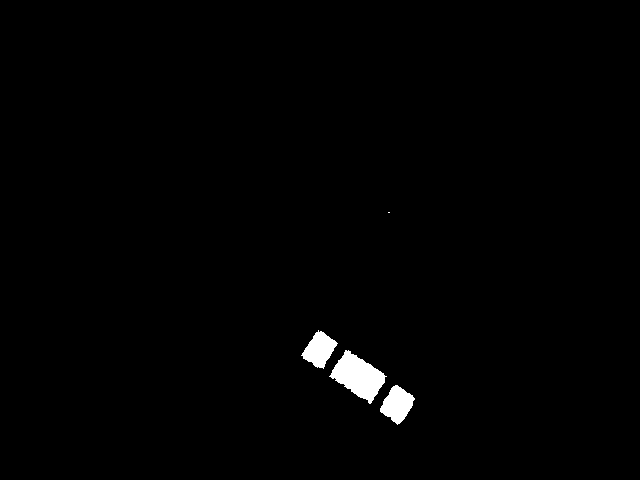
\includegraphics[width=\textwidth]{imaxes/IMPLEMENTACION/meta_a_mascara.png}
        \caption{Máscara del color de la meta}
        \label{fig:deteccion-meta-a}
    \end{subfigure}
    \hfill
    \begin{subfigure}[b]{0.32\textwidth}
        \centering
        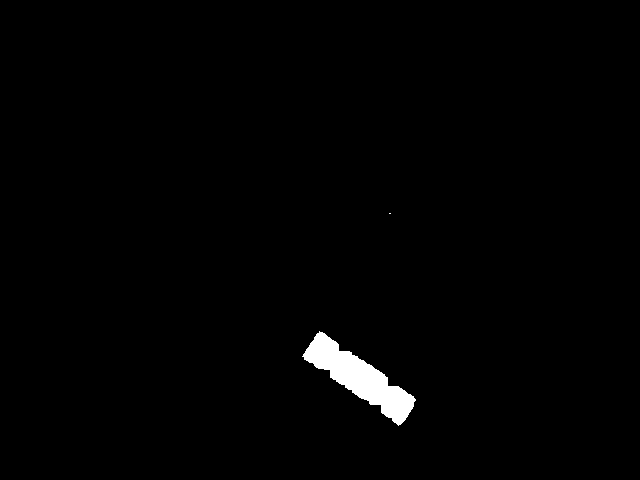
\includegraphics[width=\textwidth]{imaxes/IMPLEMENTACION/meta_b_cierre.png}
        \caption{Tras el cierre morfológico}
        \label{fig:deteccion-meta-b}
    \end{subfigure}
    \hfill
    \begin{subfigure}[b]{0.32\textwidth}
        \centering
        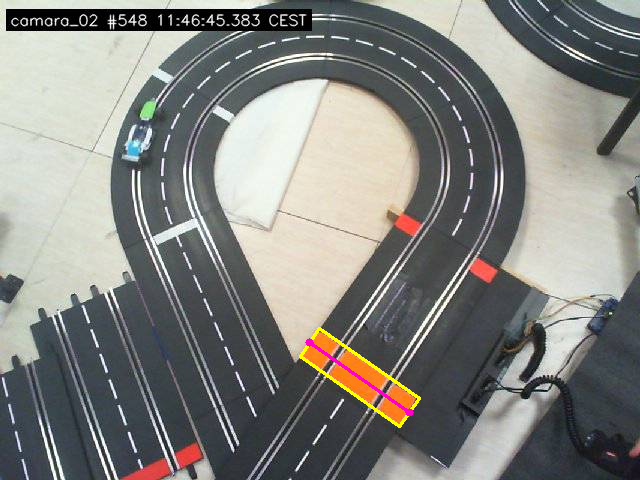
\includegraphics[width=\textwidth]{imaxes/IMPLEMENTACION/meta_c_segmento.png}
        \caption{Rectángulo y segmento}
        \label{fig:deteccion-meta-c}
    \end{subfigure}
    \caption{Detección de la línea de meta en la cámara~2. Los raíles parten la etiqueta en tres trozos que el cierre morfológico vuelve a unir; sobre la región resultante se ajusta el rectángulo de área mínima, rotado, y los puntos medios de sus lados cortos dan el segmento de meta.}
    \label{fig:deteccion-meta}
\end{figure}

Cada nodo la busca al arrancar y, si no la ve, no publica línea de meta alguna. Por lo que en un despliegue multicámara solo lo hace la que observa la linea y generando el mensaje correspondiente (tabla~\ref{tab:mensajes}). No hay, por tanto, una cámara de meta designada de antemano por el usuario.

 \chapter{Detalle del nodo de potencia}
\label{chap:anexo-actuacion}

\lettrine{E}{n} este anexo se detalla el nodo de potencia, resumido en la sección~\ref{sec:sistema-actuacion}. El nodo envía hacia el Arduino los valores de PWM calculados por los controladores y está formado por dos componentes, en primer lugar el nodo de potencia de ROS2, que centraliza la recepción de las consignas de todos los controladores, y en segundo lugar el subsistema hardware, compuesto por la placa Arduino y el módulo controlador de motores (L293D).

\section{Tratamiento de las consignas recibidas}
\label{subsec:actuacion-topics}

El nodo de potencia es un nodo puramente consumidor, no publica nada, se limita a suscribirse a los \emph{topics} en los que cada controlador anuncia el PWM de su carril. Las suscripciones se generan dinámicamente, una por cada coche declarado en la lista de configuración, \ref{subsec:params-yaml}.

De cada mensaje extrae el identificador del carril y su valor de PWM, y le aplica dos comprobaciones antes de mandarlo al puerto serie. La primera es un filtro de repetición, el nodo guarda el último valor enviado a cada carril y descarta el mensaje si coincide con él. Como los controladores publican una consigna por cada posición recibida y el PWM se mantiene estable durante tramos enteros del circuito, este filtro reduce drásticamente el tráfico sobre el puerto. La segunda es una validación del rango admitido por el hardware, entre 0 y 255, como última barrera frente a consignas mal formadas.

%El nodo se suscribe también al \emph{topic} de calibración de cada coche que esté configurado para control automático. Durante esa fase es él quien aplica al carril un valor de potencia que permite tener una velocidad de calibración constante, porque los controladores todavía no publican consigna alguna. En cuanto un coche cierra su vuelta se pasa a aplicar el valor que publica el controlador. Los carriles de los coches marcados como manuales no se tocan en ningún momento.
El nodo se suscribe también al \emph{topic} de calibración de cada coche que no esté configurado para control manual, es decir los modos incremental, automático y por política. Durante esa fase es él quien aplica al carril un valor de potencia que permite tener una velocidad de calibración constante, porque los controladores todavía no publican consigna alguna. En cuanto un coche cierra su vuelta se pasa a aplicar el valor que publica el controlador. Los carriles de los coches marcados como manuales no se tocan en ningún momento.

\section{Comunicación con el Arduino}
\label{subsec:actuacion-interfaz}

La comunicación con la placa se encapsula, como en el trabajo de Adrián Rego~\cite{tfgadrian}, en una clase independiente que forma parte del nodo y que abstrae, la complejidad de la comunicación con el puerto serie, en operaciones de alto nivel: fijar la velocidad de un carril, la de ambos o detenerlos. Al inicializarse enumera los puertos disponibles y, si el configurado no está, toma el primer dispositivo compatible que encuentre; después espera a que la placa termine de reiniciarse, vacía el búfer de entrada y detiene ambos carriles, de modo que el sistema arranca siempre desde un estado seguro.

%El protocolo es textual. %y mínimo. Cada orden es una línea de la forma \texttt{r<carril>\allowbreak :<valor>}, por ejemplo \texttt{r1:120}, donde el primer campo identifica el carril y el segundo el PWM a aplicar. El envío es bloqueante, tras escribir la orden la interfaz espera la confirmación de la placa (\texttt{OK}) y solo entonces da la operación por completada; si no llega dentro del tiempo límite, el envío se considera fallido. Aquí ese carácter bloqueante es lo que serializa el acceso.
El protocolo es textual. Cada orden es una línea de la forma \texttt{r<carril>\allowbreak :<valor>}, por ejemplo \texttt{r1:120} fija el carril 1 en un PWM de 120. El envío es bloqueante, la orden no se da por completada hasta que la placa responde con su confirmación (\texttt{OK}), y ese bloqueo es lo que serializa el acceso al puerto.

\section{Subsistema hardware}
\label{subsec:actuacion-hardware}

El subsistema hardware traduce las órdenes recibidas por el puerto serie en la tensión que se aplica sobre los raíles. El montaje es el del trabajo de Adrián Rego~\cite{tfgadrian} y se reutiliza sin cambios. La placa se conecta al ordenador por USB, que es a la vez el canal serie y la alimentación de los motores, y del módulo controlador parten hacia la pista una masa común y dos salidas de potencia, una por carril. Los componentes se describen en la sección~\ref{sec:tecnoloxias-hardware}.

Sobre la placa corre un firmware sencillo, cargado con el IDE de Arduino, que configura los pines de salida PWM, lee el puerto serie a la espera de órdenes y, por cada línea recibida, aplica la señal sobre el pin del carril indicado y responde con la confirmación que la interfaz espera. El ciclo de trabajo del pin es proporcional al valor recibido: 0 corresponde a un ciclo nulo, con el carril detenido, y 255 al ciclo completo; de ahí sale el rango que valida el nodo de potencia.

%Lo que aporta este trabajo no es el montaje, sino su encaje en la arquitectura distribuida. En el trabajo previo la interfaz vivía dentro de una aplicación de escritorio que era también quien procesaba las imágenes y decidía las velocidades; aquí queda detrás del nodo de potencia, el cual permite una comunicación y controla el acceso.

 \chapter{Listados de referencia}
\label{chap:listados}

\lettrine{E}{n} este anexo se recogen íntegras las definiciones de los mensajes propios del sistema (sección~\ref{subsec:mensajes-propios}) y los ficheros que definen su configuración y despliegue (sección~\ref{sec:configuracion_despliegue}). Los tres listados que se emplean como ejemplo en el cuerpo de la memoria —el mensaje \texttt{CarLocation} y el fichero de lanzamiento y el \emph{compose} del nodo de captura— están en los listados~\ref{lst:msg-carlocation}, \ref{lst:camera-launch} y~\ref{lst:compose-camera}.

\section{Definición de los mensajes}
\label{sec:anexo-mensajes}

\begin{lstlisting}[caption={Mensajes que transportan la información del sistema.}, label={lst:msgs-informacion}]
# ===== FinishLine.msg =====
# Identificar que camara vio la linea de meta
string camara_id

LineSegment finish_line

# ===== SpeedCarril.msg =====
int32 pwm
# ri -> Forma de referirnos al carril
string carril
# Marca temporal para controlar cada cuanto
# nos llegan los mensajes del robot
builtin_interfaces/Time stamp

# ===== TimePerLap.msg =====
float64 lap_time
builtin_interfaces/Time stamp
int32 lap_number

# ===== CarControlTelemetry.msg =====
float64 dist_derrape
bool estado_derrapando
# Tiempo que pasa desde que recibimos la informacion
# del coche hasta que enviamos el pwm a RaceController
float64 pipeline_time
# Momento exacto en el que llego el paquete de la
# camara al CarController
builtin_interfaces/Time receive_msg_stamp
# Para saber si estamos detectando correctamente el coche
int32 roi_size
\end{lstlisting}

\begin{lstlisting}[caption={Mensajes auxiliares, empleados como piezas de construcción de los anteriores.}, label={lst:msgs-auxiliares}]
# ===== Point2D.msg =====
float64 x
float64 y

# ===== Stiker.msg =====
Point2D center
string color

# ===== BoundingRect.msg =====
int32 x
int32 y
int32 w
int32 h

# ===== LineSegment.msg =====
Point2D start
Point2D end
\end{lstlisting}

\section{Fichero de parámetros}
\label{sec:anexo-params}

\begin{lstlisting}[caption={Fichero de parámetros común del sistema (\texttt{config/params.yaml}).}, label={lst:params-yaml}]
/**:
  ros__parameters:
    modo_calibracion: True
    # Lista de coches del sistema. Genera un detector por coche en la camara,
    # un controlador por coche y las suscripciones del puente Arduino. Cada
    # nombre de esta lista tiene que tener su bloque en 'cars' de abajo.
    coches: ["car1", "car2"]

    # Configuracion POR COCHE. La clave (car1, car2, ...) es el identificador
    # del coche y coincide con 'coches' y con el namespace ROS (/car1/...).
    # Aqui vive TODO lo que distingue a un coche de otro:
    #   - stiker_front/back: colores de sus dos pegatinas. La camara construye
    #     un ColorDetector por coche con estos colores, y por eso dos coches
    #     con colores distintos se pueden seguir a la vez sin confundirse.
    #   - carril: carril fisico del Arduino al que esta conectado este coche
    #     ("r1"/"1" o "r2"/"2"; el puente parsea ambas formas). Sustituye al
    #     antiguo reparto por orden de la lista en el launch: aqui se pone el
    #     carril REAL del montaje, no el que toque por posicion.
    #   - modo_manual: false -> coche autonomo, lo arranca BrainLaunch (que
    #     ademas lanza el arduino_bridge). true -> lo conduce una persona, lo
    #     arranca ManualLaunch (sin puente). Cada launch filtra 'coches' por
    #     este flag, asi que para un mixto (uno manual + uno autonomo) se
    #     levantan los dos docker-compose a la vez y cada uno coge su parte.
    cars:
      car1:
        stiker_front: "azul"
        stiker_back: "verde"
        carril: "2"
        modo_manual: false
      car2:
        stiker_front: "verde"
        stiker_back: "azul"
        carril: "1"
        modo_manual: true

    #Parametros para la camara
    camera:
      # Controlar el tamano de la foto que sacamos
      # CAMERA_MODES = {
      #     0: (160, 120),
      #     1: (320, 240),
      #     2: (640, 480),
      #     3: (800, 600),
      #     4: (1280, 720),
      # }
      mode: 2
      device: '0'
      # Tamano del kernel que vamos a usar para generar la mascara
      mascara_kernel_size: 25
      # Parametro que controla si estamos en modo debug o no, en caso de
      # estar en debug se envia la imagen de lo que ve la camara
      debug: True

      # Parametros para el modulo de deteccion
      # (los colores de las pegatinas NO van aqui: son por coche, en 'cars')
      detection:
        # Color de la linea del meta del circuito
        finish_line_color: "naranja"
        # Tamano del kernel que usamos para la operacion de deteccion
        kernel_size: 5
        # Area minima que tiene que tener el stiker detectado para ser valido
        min_area: 40

    # Parametros para el controlador
    controller:
      # Velocidad minima a la que podemos ir
      minimum_speed: 65
      # Velocidad maxima que podemos alcanzar aplicando el algoritmo
      maximum_speed: 90
      distancia_nodos_trayectoria: 15.0
      umbral_control_trayectoria_correcta: 60.0
      umbral_derrape_peligro: 10.0
      umbral_derrape_seguro: 9.0
      latencia_min_nodos: 1
      latencia_max_nodos: 10

    # Parametros para el Arduino
    arduino:
      port: "/dev/ttyACM0"
      baudrate: 115200
      calibration_speed: 60
\end{lstlisting}

\section{Ficheros de lanzamiento}
\label{sec:anexo-launch}

\begin{lstlisting}[language=Python, caption={Lanzamiento de los controladores y del nodo de actuación (\texttt{launch/BrainLaunch.py}).}, label={lst:brain-launch}]
from launch import LaunchDescription
from launch_ros.actions import Node
from ament_index_python.packages import get_package_share_directory
import yaml
import os


def generate_launch_description():
    pkg_share = get_package_share_directory("image_processor_pkg")
    params_file = os.path.join(pkg_share, "config", "params.yaml")

    # 1. Cargamos la lista de coches y su configuracion por coche desde el YAML
    with open(params_file, "r") as f:
        config = yaml.safe_load(f)
        params = config["/**"]["ros__parameters"]
        coches = params["coches"]
        cars = params["cars"]

    ld = LaunchDescription()

    # 2. Un controlador por cada coche AUTONOMO (modo_manual: false). Los coches
    #    marcados como manuales los arranca ManualLaunch; para una carrera mixta
    #    (uno manual + uno autonomo) se levantan los dos docker-compose a la vez
    #    y cada launch coge su subconjunto del mismo params.yaml.
    hay_autonomo = False
    for car_name in coches:
        cfg = cars[car_name]
        if cfg.get("modo_manual", False):
            continue
        hay_autonomo = True

        ld.add_action(
            Node(
                package="image_processor_pkg",
                executable="CarControllerNode.py",
                # Nombre UNICO por coche: EstrategiaPerfil nombra sus logs con el
                # nombre del nodo (derrapesLog_<nodo>_<camara>.txt); con el mismo
                # nombre dos coches se pisarian los ficheros.
                name=f"CarController_{car_name}",
                namespace=car_name,
                parameters=[
                    params_file,
                    {
                        "car_name": car_name,
                        # Carril fisico del coche (cars.<coche>.carril), no por
                        # orden de la lista: el controlador lo mete en el mensaje
                        # SpeedCarril y el arduino_bridge lo usa para el carril.
                        "carril_asignado": str(cfg["carril"]),
                        "modo_manual": False,
                    },
                ],
                respawn=True,
                respawn_delay=2.0,
            )
        )

    # 3. El arduino_bridge solo se lanza si hay algun coche autonomo que mande
    #    PWM. Si todos los coches son manuales, no aporta nada y no se arranca.
    if hay_autonomo:
        ld.add_action(
            Node(
                package="image_processor_pkg",
                executable="RaceControllerNode.py",
                name="arduino_bridge",
                parameters=[params_file],
            )
        )

    return ld
\end{lstlisting}

\begin{lstlisting}[language=Python, caption={Lanzamiento en modo manual, sin nodo de actuación (\texttt{launch/ManualLaunch.py}). Se omite la cabecera de documentación del fichero.}, label={lst:manual-launch}]
from launch import LaunchDescription
from launch_ros.actions import Node
from ament_index_python.packages import get_package_share_directory
import yaml
import os


def generate_launch_description():
    pkg_share = get_package_share_directory("image_processor_pkg")
    params_file = os.path.join(pkg_share, "config", "params.yaml")

    # 1. Cargamos la lista de coches y su configuracion por coche desde el YAML
    with open(params_file, "r") as f:
        config = yaml.safe_load(f)
        params = config["/**"]["ros__parameters"]
        coches = params["coches"]
        cars = params["cars"]

    ld = LaunchDescription()

    # 2. Un controlador por coche MANUAL (modo_manual: true), igual que en
    #    BrainLaunch pero en manual. carril_asignado se mantiene aunque en
    #    manual no se use (publicar_velocidad sale antes): asi el nodo es el
    #    mismo en los dos modos y el mensaje SpeedCarril sigue llevandolo.
    for car_name in coches:
        cfg = cars[car_name]
        if not cfg.get("modo_manual", False):
            continue

        ld.add_action(
            Node(
                package="image_processor_pkg",
                executable="CarControllerNode.py",
                name=f"CarControllerManual_{car_name}",
                namespace=car_name,
                parameters=[
                    params_file,
                    {
                        "car_name": car_name,
                        "carril_asignado": str(cfg["carril"]),
                        "modo_manual": True,
                    },
                ],
                respawn=True,
                respawn_delay=2.0
            )
        )

    # 3. Aqui NO va el arduino_bridge: ver el punto 1 de la cabecera.

    return ld
\end{lstlisting}

\section{Ficheros de despliegue en contenedores}
\label{sec:anexo-compose}

\begin{lstlisting}[caption={Despliegue de los controladores y del nodo de actuación en la máquina conectada al Arduino (\texttt{docker-compose-brain.yml}).}, label={lst:compose-brain}]
services:
  cerebro:
    build: .
    network_mode: "host"
    privileged: true
    ipc: "host"
    pid: "host"
    devices:
      - "/dev/ttyACM0:/dev/ttyACM0"
    environment:
      - ROS_DOMAIN_ID=42
      - ROS_LOCALHOST_ONLY=0
      # Sin esto el contenedor va en UTC (ros:humble viene asi) y las marcas
      # de hora de los logs del algoritmo (derrapesLog_*.txt) salen
      # desfasadas respecto al reloj del PC y respecto al analisis, que corre
      # fuera del contenedor. Los stamps de los mensajes NO se ven afectados:
      # son epochs y las restas entre ellos dan igual el huso
      - TZ=Europe/Madrid
    volumes:
      # La zona horaria del host, ya compilada: glibc la lee aunque la imagen
      # no tuviese tzdata. Va junto a TZ porque cada mecanismo cubre un hueco
      # del otro (ver comentario de arriba)
      - /etc/localtime:/etc/localtime:ro
      - ./src/image_processor_pkg:/ros2_ws/src/image_processor_pkg
    command: >
      bash -c "source /opt/ros/humble/setup.bash &&
               colcon build --symlink-install &&
               source install/setup.bash &&
               ros2 launch image_processor_pkg BrainLaunch.py"
\end{lstlisting}

\begin{lstlisting}[caption={Despliegue en modo manual: sin acceso al Arduino y sin nodo de actuación (\texttt{docker-compose-manual.yml}).}, label={lst:compose-manual}]
# Despliegue del cerebro para una CARRERA MANUAL (la conduce una persona con
# el mando fisico del Scalextric). Es docker-compose-brain.yml con dos
# diferencias:
#
#   1. Sin el bloque `devices`: aqui el Arduino no se usa (queda fuera del
#      circuito), asi que el contenedor arranca aunque no este ni conectado.
#   2. Lanza ManualLaunch.py, que arranca los mismos controladores pero SIN
#      el arduino_bridge y con modo_manual=True.
#
# Uso:  docker compose -f docker-compose-manual.yml up
services:
  cerebro:
    build: .
    network_mode: "host"
    privileged: true
    ipc: "host"
    pid: "host"
    environment:
      - ROS_DOMAIN_ID=42
      - ROS_LOCALHOST_ONLY=0
      - TZ=Europe/Madrid
    volumes:
      - /etc/localtime:/etc/localtime:ro
      # Monta el paquete desde el host: sin esto los derrapesLog_*.txt que
      # escribe el algoritmo (en src/image_processor_pkg/logs_carrera) se
      # perderian al parar el contenedor, y son justo lo que hay que pasarle
      # al analisis para ver que habria hecho el algoritmo
      - ./src/image_processor_pkg:/ros2_ws/src/image_processor_pkg
    command: >
      bash -c "source /opt/ros/humble/setup.bash &&
               colcon build --symlink-install &&
               source install/setup.bash &&
               ros2 launch image_processor_pkg ManualLaunch.py"
\end{lstlisting}

%\include{anexos/...}

 \printglossary[type=\acronymtype,title=\nomeglosarioacronimos]
 \printglossary[title=\nomeglosariotermos]

 \bibliographystyle{IEEEtranN}
 \bibliography{\bibconfig,bibliografia/bibliografia}
 \clearpage
 
\end{document}

%%%%%%%%%%%%%%%%%%%%%%%%%%%%%%%%%%%%%%%%%%%%%%%%%%%%%%%%%%%%%%%%%%%%%%%%%%%%%%%%
